%%%%%%%%%%%%%%%%%
%Problems include
%%%%%%%%%%%%%%%%%
%-References
%-Inconsistent notation
%-Implicit assumptions (e.g., iid)
%-Inconsistently pitched level
%-Stuff missing
%-Inconsistent inclusion of fact vs. proof/intuition
%-Some special cases explicit; others implicit
%-Organization is mix of chronological and thematic
%-Inconsistent formatting
%
%
%%%%%%%%%%%%%%%%%
%Things to (potentially) add include
%%%%%%%%%%%%%%%%%
%-End of Nir
%-Confidence intervals
%-Bootstrap
%-Levin math notes
%-More Bernheim notes
%-Manuel notes
%-Metrics: indirect Wald; NLLS consistency requires linearity in endogenous variables otherwise must instrument (see MaCurdy P.S. 2); QML only OK if linear in endogenous (and errors)

\documentclass[8pt,letterpaper, landscape]{extarticle} % using extarticle instead of article to get smaller fonts; should be used with three columns
%\documentclass[10pt,letterpaper, landscape]{article} % Full sized font version; should be used with two columnsf

\usepackage{intcheatsheet}

% Shortcuts for Script X, Y, and B and bold A, B, C, X, I, 0, ...
\newcommand{\B}{\ensuremath{\mathcal{B}}}
\newcommand{\X}{\ensuremath{\mathcal{X}}}
\newcommand{\Y}{\ensuremath{\mathcal{Y}}}
\newcommand{\mA}{\ensuremath{\mathbf{A}}}
\newcommand{\mB}{\ensuremath{\mathbf{B}}}
\newcommand{\mC}{\ensuremath{\mathbf{C}}}
\newcommand{\mD}{\ensuremath{\mathbf{D}}}
\newcommand{\mX}{\ensuremath{\mathbf{X}}}
\newcommand{\mY}{\ensuremath{\mathbf{Y}}}
\newcommand{\mx}{\ensuremath{\mathbf{x}}}
\newcommand{\my}{\ensuremath{\mathbf{y}}}
\newcommand{\mI}{\ensuremath{\mathbf{I}}}
\newcommand{\mi}{\ensuremath{\mathbf{\iota}}}
\newcommand{\mmu}{\ensuremath{\mathbf{\mu}}}
\newcommand{\mc}{\ensuremath{\mathbf{c}}}
\newcommand{\mSigma}{\ensuremath{\mathbf{\Sigma}}}
\newcommand{\mzero}{\ensuremath{\mathbf{0}}}

\renewcommand{\ln}{\log}

%%%%%%%%%%%%%%%%%%%%%%%%%%%%%%%%%%%%%%%%%%%%%%%%%%%%%%%%%%%%%%%%%%%%%%%%%%%%%%%%%%%%%

\begin{document}
\noindent Luke Stein \\
%\footnote{Most content is copied verbatim (or only minimally rewritten) from a variety of sources; errors in the source materials are now in the good company of numerous additional errors I have presumably introduced in writing/compiling these notes.}
Stanford graduate economics core (2006--7) \\
Reference and review (last updated April 11, 2012)
\hrule
%%%%%%%%%%%%%%%%%%%%%%%%%%
\setlength\columnseprule{.4pt} % Set vertical rules between columns
\begin{multicols}{4}
\cftpagenumbersoff{subsubsection} % Turn off page numbers for subsections (headers) in the TOC
\tableofcontents
\end{multicols}
%\newpage % pagebreak to use instead of rule
\hrule % rule to use instead of page break
%%%%%%%%%%%%%%%%%%%%%%%%%%
\setlength\columnseprule{0pt} % Clear vertical rules between columns
\begin{multicols}{3}
%\begin{multicols*}{2}
\section{Econometrics}
\begin{description}
\subsection{Probability foundations}
\litem{Basic set theory}{C\&B 1.1.4} All sets $ A, B, C $ satisfy:
\begin{enumerate}
\item Commutativity\index{Commutativity}: $ A \cup B = B \cup A $ and $ A \cap B = B \cap A $;
\item Associativity\index{Associativity}: $ A \cup (B \cup C) = (A \cup B) \cup C $ and $ A \cap (B \cap C) = (A \cap B) \cap C $;
\item Distributive laws\index{Distributive laws}: $ A \cap (B \cup C) = (A \cap B) \cup (A \cap C) $ and $ A \cup (B \cap C) = (A \cup B) \cap (A \cup C) $;
\item DeMorgan's Laws\index{DeMorgan's Laws}: $ (A \cup B)^{\mathsf{C}} = A^{\mathsf{C}} \cap B^{\mathsf{C}} $ and $ (A \cap B)^{\mathsf{C}} = A^{\mathsf{C}} \cup B^{\mathsf{C}} $.
\end{enumerate}

\litem{Disjointness}{C\&B 1.1.5} Two events are disjoint (a.k.a.\ mutually exclusive\index{Mutual exclusivity}) iff $ A \cap B = \emptyset $. Events $ \{ A_i \} $ are pairwise disjoint or mutually exclusive iff $ A_i \cap A_j = \emptyset $ for all $ i \neq j $. Two events with nonzero probability cannot be both mutually exclusive and independent (see ex.~1.39).

\litem{Partition}{C\&B 1.1.6} $ A_1, A_2, \dotsc $ is a partition of $ S $ iff:
\begin{enumerate}
\item $ S = \bigcup_i A_i $ (i.e., covering);
\item $ A_1, A_2, \dotsc $ are pairwise disjoint (i.e., non-overlapping).
\end{enumerate}

\litem{Sigma algebra}{C\&B 1.2.1} Collection of subsets of $ S $ (i.e., a subset of the power set of $ S $) is a sigma algebra, denoted \B{} iff:
\begin{enumerate}
\item $ \emptyset \in \B $;
\item If $ A \in \B $, then $ A^{\mathsf{C}} \in \B $ (closed under complementation---along with first axiom gives $ S \in \B $);
\item If $ \{ A_i \} \subseteq \B $, then $ \bigcup_i A_i \in \B $ (closed under countable unions).
\end{enumerate}
A cdf completely determines the probability distribution of a random variable if its probability function is defined only for events in the Borel field $ \B^1 $\index{Borel field}\index{B1 (Borel field)@$ \B^1 $ (Borel field)}, the smallest sigma algebra containing all the intervals of real numbers of the form $ (a, b)$, $[a, b)$, $(a, b]$, $[a,b]$. If probabilities are defined for a larger class of events, two random variables \textit{may} have the same cdf but not the same probability for every event (see C\&B p.~33).

\litem{Probability function}{C\&B 1.2.4, 8--9, 11} Given a sample space $ S $ and associated sigma algebra \B, a function $ P \colon \B \to \R  $ is a probability function iff it satisfies the Kolmogorov Axioms or Axioms of Probability\index{Kolmogorov Axioms or Axioms of Probability}\index{Axioms of Probability}:
\begin{enumerate}
\item $ P(A) \geq 0 $ for all $ A \in \B $;
\item $ P(S) = 1 $;
\item If $ \{ A_i \} \subseteq \B $ are pairwise disjoint, then $ P(\bigcup_i A_i) = \sum_i P(A_i) $ (countable additivity for pairwise disjoint sets).
\end{enumerate}
For any probability function $ P $ and $ A, $ $ B \in \B $,
\begin{enumerate}
\item $ P(\emptyset) = 0 $;
\item $ P (A) \leq 1 $;
\item $ P(A^{\mathsf{C}}) = 1 - P(A) $;
\item $ P (B \cap A^{\mathsf{C}}) = P(B) - P (A \cap B) $ ($B$ but not $A$ is $ B $ minus both $ A $ and $ B $);
\item $ P (A \cup B) = P(A) + P(B) - P(A \cap B) $;
\item If $ A \subseteq B $, then $ P(A) \leq P(B) $.
\end{enumerate}
If $ \{ C_i \} $ partitions $ A $, then $ P(A) = \sum_i P(A \cap C_i) $.

\litem{Probability space}{Hansen 1-31, 1-28} $ (\Omega, \mathcal{F}, P) $ where:
\begin{enumerate}
\item $ \Omega $ is the universe (e.g., $ S $, the sample space);
\item $ \mathcal{F} $ is the $ \sigma $-field (e.g., $ \B^1 $);
\item $ P $ a probability measure (e.g., $ \mathcal{P} $, the probability measure that governs all random variables).
\end{enumerate}
A random variable $ X $ induces a probability measure $ P_X $ defined by $ P_X (B) \equiv P(X \in B) = P(F) $. This gives the probability space $ (\R, \B, P_X) $.

\litem{Counting}{C\&B sec.~1.2.3} The number of possible arrangement of size $ r $ from $ n $ objects is
\begin{center}
\begin{tabular}{ccc}
\hline
 & No replacement & With replacement \\
Ordered & $ \frac{n!}{(n-r)!} $ & $ n^r $ \\
Unordered & $ \binom{n}{r} $ & $ \binom{n+r-1}{r} $  \\
\hline
\end{tabular}
\end{center}
where $ \binom{n}{r} \equiv \frac{n!}{r! (n-r)!} $. (Unordered with replacement, a.k.a.\ ``stars and bars.''\index{Stars and bars@``Stars and bars''})

\litem{Conditional probability}{C\&B 1.3.2, ex.~1.38} For $ A $, $ B \in S $ with $ P(B) > 0 $, the conditional probability of $ A $ given $ B $ is $ P(A|B) \equiv P(A \cap B) / P(B) $.
\begin{enumerate}
\item If $ A $ and $ B $ are disjoint ($ A \cap B = \emptyset $), then $ P(A|B) = P(B|A) = 0 $.
\item If $ P(B) = 1 $, then $ \forall A, P(A|B) = P(A) $.
\item If $ A \subseteq B $, then $ P(B|A) = 1 $ and $ P(A|B) = P(A)/P(B) $.
\item If A and B are mutually exclusive, $ P(A|A \cup B) = P(A) / [P(A) + P(B)] $.
\item $ P (A \cap B \cap C) = P(A|B \cap C) \cdot P(B|C) \cdot P(C) $.
\end{enumerate}

\litem{Bayes' Rule}{C\&B 1.3.5} A formula for ``turning around'' conditional probabilities: $ P (A|B) = P(B|A) \cdot P(A) / P(B) $. More generally, if $ \{ A_i \} $ partition the sample space and $ B $ is any set, then $ \forall i, $ $$ P(A_i | B) = \frac{P(B|A_i) \cdot P(A_i)}{\sum_j P(B|A_j) \cdot P(A_j)}. $$

\litem{Independence of events}{C\&B 1.3.7, 9, 4.2.10}\index{Independent} $ A $, $ B $ statistically independent iff $ P(A \cap B) = P(A) \cdot P(B) $ or identically iff $ P(A|B) = P(A) $ (this happens iff $ P(B|A) = P(B) $).
\begin{enumerate}
\item Iff $ A $ and $ B $ are independent, then the following pairs are also independent: $ A $ and $ B^{\mathsf{C}} $, $ A^{\mathsf{C}} $ and $ B $, $ A^{\mathsf{C}} $ and $ B^{\mathsf{C}} $.
\item Two events with nonzero probability cannot be both mutually exclusive and independent (see ex.~1.39).
\item If $ X $, $ Y $ independent r.v.s, then for any $ A $, $ B \subseteq \R $, events $ \{ X \in A \} $ and $ \{ Y \in B \} $ are independent events.
\end{enumerate}

\litem{Mutual independence of events}{C\&B 1.3.12}\index{Independent} A collection of events $ \{ A_i \} $ are mutually independent iff for any subcollection $ A_{i_1}, \dotsc, A_{i_k} $ we have $ P (\bigcap_j A_{i_j}) = \prod_j P(A_{i_j}) $. Note that pairwise independence does \textit{not} imply mutual independence.

\subsection{Random variables}
\litem{Random variable}{1.4.1, 1.5.7--8, 10, sec.~3.2} A function $ X \colon S \to \R $ where $ S $ is a sample space.
\begin{enumerate}
\item Continuous\index{Continuous r.v.} iff its cdf is a continuous function and discrete\index{Discrete r.v.} iff its cdf is a step function (i.e., if sample space is countable).
\item Identically distributed iff $ \forall A \in \B^1, $ $ P(X \in A) = P (Y \in A) $, or identically iff $ \forall x, $ $ F_X(x) = F_Y(x) $.
\item Note identical distribution says nothing about (in)dependence.
\end{enumerate}

\litem{Random vector}{C\&B 4.1.1} $ n $-dimensional random vector is a function $ \mX \colon S \to \R^n $ where $ S $ is a sample space.

\litem{Measurability}{Hansen 1-28, 4-11} A r.v.\ $ X \colon (\Omega, \mathcal{F}) \to (\R, \mathcal{B}) $ is $ \mathcal{F} $-measurable iff $ \forall B \in \mathcal{B} $, $ \{ \omega \in \Omega \colon X(\omega) \in B \} \in \mathcal{F} $ (i.e., the preimage of every element of $ \mathcal{B} $ is an element of $ \mathcal{F} $).

If $ \mathcal{F} $ and $ \mathcal{G} $ are both $ \sigma $-fields with $ \mathcal{G} \subseteq \mathcal{F} $, then $ X $ is $ \mathcal{G} $-measurable $ \implies X $ is $ \mathcal{F} $-measurable (i.e., if the preimage of every $ B $ is in $ \mathcal{G} $, it is also in its superset $ \mathcal{F} $).

\litem{Smallest $ \sigma $-field}{Hansen 4-12} The smallest $ \sigma $-field that makes a r.v.\ $ Z \colon (\Omega, \mathcal{F}) \to (\R, \B) $ measurable is $ \sigma (Z) \equiv \{ G \subseteq \Omega \colon \exists B \in \B $, $ G = Z^{-1} (B) \} $ (i.e., the set of preimages of elements of $ \B $).

\litem{Independence of r.v.s}{C\&B 4.2.5, 7, p.~154, 4.3.5}\index{Independent} $ X $ and $ Y $ independent r.v.s (written $ X \independent Y $) iff any of the following equivalent conditions hold:
\begin{enumerate}
\item $ \forall A $, $ B $, $ P (X \in A $, $ Y \in B) = P (X \in A) \cdot P (Y \in B) $.
\item $ F_{XY} (x,y) \equiv P (X \leq x $, $ Y \leq y) = F_X (x) F_Y(y) $.
\item $ f(x,y) = f_{X}(x) f_Y(y) $ (i.e., joint pdf/pmf is the product of marginal pdfs/pmfs).
\item $ f(y|x) = f_Y(y) $ (i.e., conditional pdf/pmf equals marginal pdf/pmf).
\item $ \exists g(x) $, $ h(y) $, $ \forall x $, $ y $, $ f(x,y) = g(x) h(y) $ (i.e., joint pdf/pmf is separable). Note that functional forms may appear separable, but limits may still depend on the other variable; if the support set of $ (X,Y) $ is not a cross product, then $ X $ and $ Y $ are \textit{not} independent.
\end{enumerate}
For any functions $ g(t) $ and $ h(t) $, $ X \independent Y \implies g(X) \independent h(Y) $.

\litem{Independence of random vectors}{C\&B 4.6.5}\index{Independent} $ \mX_1 , \dotsc , \mX_n $ mutually independent iff for every $ ( \mx_1 , \dotsc , \mx_n ) $, the joint pdf/pmf is the product of the marginal pdfs/pmfs; i.e.,
$ f ( \mx_1 , \dotsc , \mx_n ) = \prod_i f_{\mX_i} (\mx_i)$.
\begin{enumerate}
\item Knowledge about the values of some coordinates gives us no information about the values of the other coordinates.
\item The conditional distribution of any subset of the coordinates, given the values of the rest of the coordinates, is the same as the marginal distribution of the subset.
\item Mutual independence implies pairwise independence, but pairwise independence does \textit{not} imply mutual independence.
\end{enumerate}

\litem{Mean independence}{Metrics P.S. 3-4c, Metrics section} $ X $ is mean independent of $ Y $ (written $ X \independentm Y $) iff $ \E (X|Y) = \E (X) $.
\begin{enumerate}
\item Mean independence is not transitive (i.e., $ X \independentm Y $ does \textit{not} imply that $ Y \independentm X $).
\item Independence implies mean independence (i.e., $ X \independent Y \implies X \independentm Y \land Y \independentm X  $).
\item $ X \independentm Y \implies \E [(X | g(Y)] = \E [X] $, for any function $ g (\cdot) $.
\item $ X \independentm Y \implies \Cov (X, g(Y)) = 0 $ for any function $ g (\cdot) $.
\end{enumerate}

\litem{Cumulative distribution function}{C\&B 1.5.1, 3, p.~147}\index{cdf (cumulative distribution function)} $ F_X(x) \equiv P(X \leq x) $. By the Fundamental Theorem of Calculus, $ \frac{d}{dx} F_X(x) = f_X(x) $ for a continuous r.v.\ at continuity points of $ f_X $. A function $ F $ is a cdf iff:
\begin{enumerate}
\item $ \lim_{x \to -\infty} F(x) = 0 $ and $ \lim_{x \to \infty} F(x) = 1 $;
\item $ F (\cdot) $ nondecreasing;
\item $ F (\cdot) $ right-continuous; i.e., $ \forall x_0 $, $ \lim_{x \downarrow x_0} F(x) = F(x_0) $.
\end{enumerate}
A random vector $ X $ has joint cdf\index{Joint cdf} $ F_X(x_1, \dotsc, x_n) \equiv P (X_1 \leq x_1, \dotsc, X_n \leq x_n) $. By the Fundamental Theorem of Calculus, $ \frac{\partial^n}{\partial x_1 \dotsm \partial x_n} F_X(\vec{x}) = f_X(\vec{x}) $ for a continuous (in all dimensions) random vector at continuity points of $ f_X $.

\litem{Probability mass function}{C\&B 1.6.1, 5, 4.1.3}\index{pmf (probability mass function)} For a discrete r.v., $ f_X (x) \equiv P (X = x) $. A function $ f_X $ is a pmf iff:
\begin{enumerate}
\item $ \forall x, $ $ f_X(x) \geq 0 $;
\item $ \sum_x f_X(x) = 1 $.
\end{enumerate}
$ f_X $ gives the probability of any event: $ P (X \in B) = \sum_k 1_{(x_k \in B)} f_X(x_k) $.

A discrete random vector $ X $ has joint pmf\index{Joint pmf} $ f_X(\vec{v}) \equiv P (X = \vec{v}) $.

\litem{Marginal pmf}{C\&B 4.1.6, p.~178} For a discrete random vector,
%$ f_{X_i} (x) \equiv P(X_i = x) = $
%$$ \sum_{(x_1, \dotsc, x_{i-1}, x_{i+1}, \dotsc, x_n) \in \R^{n-1}} f_X (x_1, \dotsc, x_{i-1}, x, x_{i+1}, \dotsc, x_n), $$
$$ f_{X_i} (x_i) \equiv P(X_i = x_i) = \sum_{x_{-i} \in \R^{n-1}} f_X (x) ; $$
i.e., hold $ X_i = x_i $, and sum $ f_X $ over all remaining possible values of $ X $.

We can also take the marginal pmf for multiple $ i $ by holding these and summing $ f_X $ over all remaining possible values of $ X $.

\litem{Conditional pmf}{C\&B 4.2.1} For $ (X,Y) $ a discrete random vector, $ f(y|x) \equiv P(Y = y | X = x) = f(x,y)/f_X(x) $, where $ f(x,y) $ is joint pmf, and $ f_X(x) $ is marginal pmf.

\litem{Probability density function}{C\&B 1.6.3, 5, 4.1.10}\index{pdf (probability density function)} For a continuous r.v., $ f_X (x) $ defined as the function which satisfies $ F_X(x) = \int_{-\infty}^{x} f_X(t) \, dt $ for all $ x $. A function $ f_X $ is a pdf iff:
\begin{enumerate}
\item $ \forall x $, $ f_X(x) \geq 0 $;
\item $ \int_\R f_X(x) \, dx = 1 $.
\end{enumerate}
$ f_X $ gives the probability of any event: $ P (X \in B) = \int_\R 1_{(x \in B)} f_X(x) \, dx $.

A continuous (in all dimensions) random vector $ X $ has joint pdf\index{Joint pdf} $ f_X(x_1, \dotsc, x_n) $ iff $ \forall A \subseteq \R^n, $ $ P(X \in A) = \idotsint_A f_X(x_1, \dotsc, x_n) \, dx_1 \dotsm dx_n $.

\litem{Marginal pdf}{C\&B p.~145, 178} For a  continuous (in all dimensions) random vector,
$$ f_{X_i} (x_i) \equiv \idotsint_{\R^{n-1}} f_X (x) \, dx_1 \dotsm dx_{i-1} \, dx_{i+1} \dotsm dx_n, $$
i.e., hold $ X_i = x_i $, and integrate $ f_X $ over $ \R $ in all $ X_j $ for $ i \neq j $.

We can also take the marginal pdf for multiple $ i $ by holding these and integrating $ f_X $ over $ \R $ in all $ X_j $ that aren't being held.

\litem{Conditional pdf}{C\&B 4.2.3, p.~178} For $ (X,Y) $ a continuous random vector, $ f(y|x) \equiv f(x,y)/f_X(x) $ as long as $ f_X(x) \neq 0 $, where $ f(x,y) $ is joint pdf, and $ f_X(x) $ is marginal pdf.

We can also condition for/on multiple coordinates: e.g., for $ (X_1, X_2, X_3, X_4) $ a continuous random vector, $ f(x_3, x_4|x_1, x_2) \equiv f(x_1, x_2, x_3, x_4) / f_{X_1 X_2}(x_1, x_2) $, where $ f $ is a joint pdf, and $ f_{X_1 X_2} $ is the marginal pdf in $ X_1 $ and $ X_2 $.

\litem{Borel Paradox}{4.9.3} Be careful when we condition on events of probability zero: two events of probability zero may be equivalent, but the probabilities conditional on the two events is different!

\litem{Stochastic ordering}{C\&B ex.~1.49, ex.~3.41-2} cdf $ F_X $ stochastically greater than cdf $ F_Y $ iff $ F_X(t) \leq F_Y(t) $ at all $ t $, with strict inequality at some $ t $. This implies $ P (X > t) \geq P (Y > t) $ at all $ t $, with strict inequality at some $ t $.

A family of cdfs $ \{ F(x|\theta) \} $ is stochastically increasing in $ \theta $ iff $ \theta_1 > \theta_2 \implies F(x | \theta_1) $ stochastically greater than $ F(x | \theta_2) $. A location family is stochastically increasing in its location parameter; if a scale family has sample space $ [0, \infty) $, it is stochastically increasing in its scale parameter.

\litem{Support set}{C\&B eq.~2.1.7}\index{Support} Support set (a.k.a.\ support) of a r.v.\ $ X $ is $ \X \equiv \{ x \colon f_X(x) > 0 \} $, where $ f_X $ a cdf or pdf (or in general, any nonnegative function).

\subsection{Transformations of random variables}
\litem{Transformation $ \R^1 \to \R^1 $}{C\&B 2.1.3, 5, 8} A discrete r.v.\ can be transformed into a discrete r.v. A continuous r.v.\ can be transformed into either a continuous or a discrete r.v.\ (or mixed!). When $ Y = g(X) $ and $ \Y \equiv g(\X) $ (where $ \X $ is the support of $ X $),
\begin{enumerate}
\item If $ g $ monotone increasing on $ \X $, then $ F_Y(y) = F_X(g^{-1}(y)) $ for $ y \in \Y $;
\item If $ g $ monotone decreasing on $ \X $ \textit{and $ X $ a continuous r.v.}, then $ F_Y(y) = 1 - F_X(g^{-1}(y)) $ for $ y \in \Y $.
\end{enumerate}
If $ g $ monotone, $ f_X $ continuous on $ \X $, and $ g^{-1} $ has continuous derivative on $ \Y $, then:
$$ f_Y(y) = \begin{cases}
f_X \left( g^{-1}(y) \right) \left| \tfrac{d}{dy} g^{-1}(y) \right|, & y \in \Y; \\
0, & \text{otherwise.}
\end{cases} $$
If $ \{A_i \}_{i=0}^k $ partitions $ \X $, with $ P (X \in A_0) = 0 $; $ f_X $ continuous on each $ A_i $; and $ \exists \{A_i \}_{i=1}^k $ satisfying:
\begin{enumerate}
\item $ g(x) = g_i(x) $ for $ x \in A_i $,
\item $ g_i $ monotone on $ A_i $,
\item $ \exists \Y $, $ \forall i $, $ g_i(A_i) = \Y $ (i.e., all $ A_i $ have same image under their respective $ g_i $s) [Hansen note 2-15 suggests this need not hold],
\item $ \forall i $, $ g_i^{-1} $ has a continuous derivative on $ \Y $; then:
\end{enumerate}
$$ f_Y(y) = \begin{cases}
\sum_{i=1}^k f_X \left( g_i^{-1}(y) \right) \left| \tfrac{d}{dy} g_i^{-1}(y) \right|, & y \in \Y; \\
0, & \text{otherwise.}
\end{cases} $$

\litem{Transformation $ \R^2 \to \R^2 $}{C\&B p.~158, 185} Let $ U = g_1 (X,Y) $ and $ V = g_2 (X,Y) $ where:
\begin{enumerate}
\item $ (X,Y) $ has pdf $ f_{XY} $ and support $ \mathcal{A} $;
\item $ g_1 $ and $ g_2 $ define a 1-to-1 transformation from $ \mathcal{A} $ to $ \mathcal{B} \equiv \{ (u,v) \colon u \in g_1(\mathcal{A}) $, $ v \in g_2(\mathcal{A}) \} $ (i.e., the support of $ (U,V) $);
\item Inverse transform is $ X = h_1 (U, V) $ and $ Y = h_2 (U, V) $; then:
\end{enumerate}
$$ f_{UV}(u, v) = \begin{cases}
f_{XY} (h_1(u, v), h_2(u, v)) \left| J \right| , & (u,v) \in \mathcal{B}; \\
0, & \text{otherwise;}
\end{cases} $$
where $ J $ is the Jacobian\index{Jacobian},
$$ J \equiv \operatorname{det} \begin{bmatrix}
\tfrac{\partial x}{\partial u} & \tfrac{\partial x}{\partial v} \\
\tfrac{\partial y}{\partial u} & \tfrac{\partial y}{\partial v}
\end{bmatrix} . $$
If the transformation is not 1-to-1, we can partition $ \mathcal{A} $ into $ \{ \mathcal{A}_i \} $ such that 1-to-1 transformations exist from each $ \mathcal{A}_i $ to $ \mathcal{B} $ which map $ (x,y) \mapsto (u,v) $ appropriately. Letting $ x = h_{1i} (u, v) $ and $ y = h_{2i} (u, v) $ be the inverses, and $ J_i $ the Jacobian, on $ \mathcal{A}_i $;
$$ f_{UV}(u, v) = \begin{cases}
\sum_i f_{XY} (h_{1i}(u, v), h_{2i}(u, v)) \left| J_i \right| , & (u,v) \in \mathcal{B}; \\
0, & \text{otherwise.}
\end{cases} $$
For generalization to $ \R^n \to \R^n $ case for $ n > 2 $, see C\&B p.~185.

\litem{Convolution formulae}{C\&B 5.2.9, ex.~5.6} $ X \independent Y $ both continuous. Then:
\begin{enumerate}
\item $ f_{X+Y}(z) = \int_\R f_X(w) f_Y(z-w) \, dw $.
\item $ f_{X-Y}(z) = \int_\R f_X(w) f_Y(w-z) \, dw $.
\item $ f_{X Y}(z) = \int_\R | \tfrac{1}{w} | f_X(w) f_Y(z/w) \, dw $.
\item $ f_{X/Y}(z) = \int_\R | w | f_X(wz) f_Y(w) \, dw $.
\end{enumerate}

\litem{Probability integral transformation}{C\&B 2.1.10, ex.~2.10} If $ Y = F_X(X) $ (for $ X $ continuous) then $ Y \sim \unifnoital (0,1) $. Can be used to generate random samples from a particular distribution: generate a uniform random and apply inverse of cdf of target distribution. If $ X $ is discrete, $ Y $ is stochastically greater than $ \unifnoital (0,1) $.

\subsection{Properties of random variables}
\litem{Expected value, mean}{C\&B 2.2.1, 5--6, 4.6.6}\index{$ \mu $ (expected value)}
$$ \E g(X) \equiv \begin{cases}
\int_\R g(x) f_X (x) \, dx, & \text{if $ X $ continuous;} \\
\sum_{x \in \X} g(x) f_X (x) \, dx, & \text{if $ X $ discrete;}
\end{cases} $$
provided the integral or sum exists \textit{and} that $ \E |g(X)| \neq \infty $. For constants $ a, $ $ b, $ $ c $ and functions $ g_1, $ $ g_2 $ such that $ \E(g_1(X)), $ $ \E(g_2(X)) $ exist,
\begin{enumerate}
\item $ \E [a g_1(X) + b g_2(X) + c] = a \E(g_1(X)) + b \E(g_2(X)) + c $ (i.e., expectation is a linear operator);
\item If $ \forall x, g_1(x) \geq 0 $, then $ \E g_1 (X) \geq 0 $;
\item If $ \forall x, g_1(x) \geq g_2 (x) $, then $ \E g_1 (X) \geq \E g_2 (X) $;
\item If $ \forall x, a \leq g_1(x) \leq b $, then $ a \leq\E g_1 (X) \leq b $.
\end{enumerate}
The mean is the MSE minimizing predictor for $ X $; i.e., $ \min_b \E (X - b)^2 = \E (X - \E X)^2 $. If $ X_1, \dotsc , X_n $ mutually independent, then $ \E [ g_1(X_1) \cdot \dotsb \cdot g_n(X_n) ] = \E [ g_1(X_1)] \cdot \dotsb \cdot \E [g_n(X_n) ] $.

\litem{Conditional expectation}{C\&B p.~150; Hansen 4-14--6; Hayashi 138--9} a.k.a.\ regression of $ Y $ on $ X $.\index{Regression} $ \E (Y|X) $ is a r.v.\ which is a function of $ X $. For discrete $ (X,Y) $, $ \E (g(Y)|x) \equiv \sum_Y g(y) f(y|x) $. For continuous $ (X,Y) $, $ \E (g(Y)|x) \equiv \int_\R g(y) f(y|x) \, dy $. Conditional expected value has all the standard properties of expected value. Also:
\begin{enumerate}
\item $ \E [g(X) | X] = g(X) $ for any function $ g $.
\item $ \E [g(X) h(Y) | X] = g(X) \E [h(Y)|X] $ for any functions $ g $ and $ h $.
\item $ X \independent Y \implies \E (Y|X) = \E (Y) $ (i.e., knowing $ X $ gives us no additional information about $ \E Y $).
\item $ \E (Y|X) = \E (Y) \implies \Cov (X, Y) = 0  $
\item $ \E (Y|X) $ is the MSE minimizing predictor of $ Y $ based on knowledge of $ X $, (i.e., $ \min_{g(x)} \E [Y - g(X)]^{2} = \E [Y - \E (Y|X)]^{2} $).
\end{enumerate}
Let $ X $ be a r.v.\ that takes values in $ (\R, \B) $, let $ \mathcal{G} = \sigma (X) $ (i.e., the smallest sigma field measuring $ X $), and assume $ \E |Y| < \infty $. Conditional expected value of $ Y $ given $ X $, is defined implicitly (and non-uniquely) as satisfying:
\begin{enumerate}
\item $ \E | \E (Y|X) | < \infty $;
\item $ \E (Y|X) $ is $ \mathcal{G} $-measurable (i.e., $ Y|X $ cannot rely on more information than $ X $ does);
\item $ \forall G \in \mathcal{G} $, $ \int_G \E (Y|X) \, dP(\omega) = \int_G Y \, dP(\omega) $ (i.e., $ \E [ \E (Y|X) | X \in G] = \E [Y | X \in G ] $);
\end{enumerate}
where the notation $ \int_B \cdot \, dP_X(x) $ means $ \int_B  \cdot \, f_X(x) \, dx $ if $ X $ is continuous, and means $ \sum_{x \in B} \cdot \, f_X(x) $ if $ X $ is discrete.

\litem{Two-way rule for expectations}{C\&B p.~58, ex.~2.21} If $ Y = g(X) $, then $ \E g(X) = \E Y $; i.e., $ \int_\R g(x) f_X(x)\, dx = \int_\R y f_Y(y) \, dy $.

\litem{Law of Iterated Expectations}{C\&B 4.4.3; Hansen 4-21}\index{Iterated expectations} $ \E X = \E [ \E (X|Y)] $, provided the expectations exist. More generally, when $ \mathcal{L} \subseteq \mathcal{M} $ (i.e., $ \mathcal{L} $ contains less information, $ \mathcal{M} $ contains more),
$$ \E [X | \mathcal{L} ] = \E [ \E (X | \mathcal{M} ) | \mathcal{L} ] = \E [ \E (X | \mathcal{L} ) | \mathcal{M} ] . $$

\litem{Median}{C\&B ex.~2.17--18} $ m $ such that $ P (X \leq m) \geq \tfrac{1}{2} $ and $ P (X \geq m) \geq \tfrac{1}{2} $. If $ X $ continuous, the median minimizes absolute deviation; i.e., $ \min_a \E |X-a| = \E|X - m| $.

\litem{Mode}{C\&B ex.~2.27} $ f(x) $ is unimodal\index{Unimodality} with mode equal to $ a $ iff $ a \geq x \geq y \implies f(a) \geq f(x) \geq f(y) $ and $ a \leq x \leq y \implies f(a) \geq f(x) \geq f(y) $.
\begin{enumerate}
\item Modes are not necessarily unique.
\item If $ f $ is symmetric and unimodal, then the point of symmetry is a mode.
\end{enumerate}

\litem{Symmetric distribution}{C\&B ex.~2.25--26} If $ f_X $ is symmetric about $ a $ (i.e., $ \forall \epsilon, $ $ f_X(a + \epsilon) = f_X(a - \epsilon) $), then:
\begin{enumerate}
\item $ X $ and $ 2a - X $ are identically distributed;
\item If $ a = 0 $, then $ M_X $ is symmetric about 0;
\item $ a $ is the median;
\item If $ \E X $ exists, then $ \E X = a $.
\item For odd $ k $, the $ k $th central moment $ \mu_k $ is zero (if it exists); if the distribution is symmetric about $ 0 $, then all odd moments are zero (if they exist).
\end{enumerate}

\litem{Moment}{C\&B 2.3.1, 11; Hansen 2-37}\index{Central moment}\index{$ \mu_n $ (central moment)}\index{$ \mu_{n}' $ (moment)} For $ n \in \Z $, the $ n $th moment of $ X $ is $ \mu_{n}' \equiv \E X^n $. Also denote $ \mu_{1}' = \E X $ as $ \mu $. The $ n $th central moment is $ \mu_n \equiv \E(X - \mu)^n $.
\begin{enumerate}
\item Two different distributions \textit{can} have all the same moments, but only if the variables have unbounded support sets.
\item A distribution is uniquely determined by its moments if all moments are defined and $ \lim_{n \to \infty} \sum_{k=1}^{n} \mu_{k}' r^k / k! $ exists for all $ r $ in a neighborhood of zero.
\end{enumerate}

\litem{Variance}{C\&B 2.3.2, 4, p.~60, 4.5.6, ex.~4.58}\index{$ \sigma^2 $ (variance)} $ \Var X \equiv \mu_2 = \E (X - \E X)^2 = \E X^2 - (\E X)^2 $. Often parametrized as $ \sigma^2 $.
\begin{enumerate}
\item For constants $ a, $ $ b $, if $ \Var X \neq \infty $, then $ \Var (aX+b) = a^2 \Var X $;
\item Assuming variances exist, $ \Var (aX + bY) = a^2 \Var X + b^2 \Var Y + 2ab \Cov (X,Y) $;
\item $ \Var [Y - \E (Y|X)] = \E [\Var(Y|X)] $.
\end{enumerate}

\litem{Multivariate variance}{?} $ \Var \mX \equiv \E [ \mX \mX' ] - \E [ \mX ] \E [ \mX ]' $. Thus:
\begin{enumerate}
\item $ \Var ( \mX + \mY ) = \Var ( \mX ) + \Cov ( \mX , \mY ) + \Cov ( \mX , \mY )' + \Var ( \mY ) $;
\item $ \Var (\mA \mX) = \mA \Var ( \mX ) \mA' $.
\end{enumerate}

\litem{Conditional variance}{C\&B p.~151, 4.4.7; Greene 81--4} a.k.a.\ scedastic function.\index{Scedastic function} $ \Var (Y|X) \equiv E[ (Y - \E [Y|X] )^2 | X] = \E [Y^2 | X] - (\E [Y|X])^2 $.
\begin{enumerate}
\item $ X \independent Y \implies \Var (Y | X) = \Var (Y) $.
\item Conditional variance identity: provided the expectations exist,
$$ \Var (Y) = \underbrace{\E [\Var (Y|X)]}_{\text{residual variance}} + \underbrace{\Var [\E (Y|X)]}_{\text{regression variance}} . $$
Implies that on average, conditioning reduces the variance of the variable subject to conditioning ($ \Var (Y) \geq \E [\Var (Y|X)] $).
\end{enumerate}

\litem{Standard deviation}{C\&B 2.3.2}\index{$ \sigma $ (standard deviation)} $ \sigma \equiv \sqrt{\Var X} $.

\litem{Covariance}{C\&B 4.5.1, 3, ex.~4.58--9; Greene 77} $ \Cov (X, Y) \equiv \E [ (X - \E X) (Y - \E Y)] = \E [ (X - \E X) Y ] = \E [ X (Y - \E Y)] = \E (XY) - (\E X )( \E Y) $. If $ X $, $ Y $, $ Z $ all have finite variances, then:
\begin{enumerate}
\item $ \Cov (X, Y) = \Cov [X, \E(Y|X)] $;
\item $ \Cov [X, Y - \E(Y|X) ] = 0 $;
\item $ \Cov (X, Y) = \E [\Cov(X, Y|Z)] + \Cov[\E(X|Z), \E (Y|Z) ] $.
\item $ \Cov (X, Y+Z) = \Cov (X, Y) + \Cov (X,Z) $.
\item $ \Cov (aX + bY , cX + dY) = ac \Var (X) + bd \Var (Y) + (ad+bc) \Cov (X,Y) $.
\end{enumerate}

\litem{Multivariate covariance}{Hansen 5-28; Hayashi 75--6} $ \Cov (\mX, \mY) \equiv \E [(\mX - \E \mX)(\mY - \E \mY)'] = \E (\mX \mY') - ( \E \mX ) (\E \mY')  $. Thus:
\begin{enumerate}
\item $ \Cov (\mA \mX, \mB \mY) = \mA \Cov (\mX, \mY) \mB' $;
\item $ \Cov (\mX, \mY) = \Cov ( \mY , \mX )' $.
\end{enumerate}

\litem{Correlation}{C\&B 4.5.2, 5, 7}\index{$ \rho $ (correlation)} $ \operatorname{Corr} (X,Y) \equiv \rho_{XY} \equiv \Cov (X,Y) / (\sigma_X \sigma_Y) $.
\begin{enumerate}
\item $ \operatorname{Corr} (a_1 X + b_1, a_2 Y + b_2) = \operatorname{Corr} (X,Y) $.
\item Correlation is in the range $ [-1,1] $, with $ \pm 1 $ indicating a perfectly linear relationship ($ +1 $ for positive slope, $ -1 $ for negative slope), by the Cauchy-Schwarz Inequality.
\item $ X \independent Y \implies \Cov (X,Y) = \rho_{XY} = 0 $ (assuming finite moments); note however that zero covariance need \textit{not} imply independence.
\end{enumerate}

\litem{Skewness}{C\&B ex.~2.28; Greene 66}\index{$ \alpha_3 $ (skewness)} $ \alpha_3 \equiv \mu_3 \cdot (\mu_2)^{-3/2} $, where $ \mu_i $ is the $ i $th central moment. Measures the lack of symmetry in the pdf. 0 for any normal, $ t $, or uniform; $ 2 $ for exponential, $ 2 \sqrt{2/r} $ for $ \chi_r^2 $, $ 2 \sqrt{a} / a $  for gamma.

\litem{Kurtosis}{C\&B ex.~2.28}\index{$ \alpha_4 $ (kurtosis)} $ \alpha_4 \equiv \mu_4 \cdot \mu_2^{-2} $, where $ \mu_i $ is the $ i $th central moment. Measures the ``peakedness'' of the pdf. $ \alpha_4 = 3 $ for any normal. (Sometimes normalized by subtracting 3.)

\litem{Moment generating function}{C\&B 2.3.6--7, 11--12, 15, 4.2.12, 4.6.7, 9}\index{mgf (moment generating function)} $ M_X(t) \equiv \E e^{tX} $ as long as the expectation exists for $ t $ in a neighborhood 0. If $ M_X $ exists, then $ \forall n \in \Z$, $ n \geq 0 $,
$$ \mu_{n}' \equiv \E X^n = \left. \frac{d^n}{dt^n} M_X(t) \right|_{t=0}. $$
\begin{enumerate}
\item It is possible for all moments to exist, but not the mgf.
\item If r.v.s have equal mgfs in some neighborhood of 0, then the variables are identically distributed (i.e., an extant mgf characterizes a distribution).
\item If the mgfs of a sequence of r.v.s converge to $ M_X $ in some neighborhood of zero, then the cdfs of the sequence converge to $ F_X $ at all points where $ F_X $ is continuous.
\item For constants $ a, $ $ b $, if $ M_X $ exists, then $ M_{aX + b} (t) = e^{bt} M_X (at) $.
\item For $ X \independent Y $, $ M_{X + Y}(t) = M_X(t) M_Y (t) $. For $ X_1, \dotsc, X_n $ mutually independent, $ M_{\sum X_i} = \prod_i M_{X_i} $.
\item For $ X_1, \dotsc, X_n $ mutually independent, $ Z \equiv (a_1 X_1 + b_1) + \dotsb + (a_n X_n + b_n) $, then $ M_{Z}(t) = (e^{t(\sum b_i)}) \prod_i M_{X_i}(a_i t) $.
\end{enumerate}

\litem{Characteristic function}{C\&B sec.~2.6.2}\index{$ \phi (\cdot) $ (characteristic function)} $ \phi_X (t) \equiv \E e^{itX} $, where $ i = \sqrt{-1} $.
\begin{enumerate}
\item The cf always exists.
\item A cf completely determines a distribution: if the cfs of a sequence of r.v.s converge to $ \phi_X $ in some neighborhood of zero, then the cdfs of the sequence converge to $ F_X $ at all points where $ F_X $ is continuous.
\item For $ X \sim \n (0,1) $, $ \phi_X (t) = e^{-t^2 /2} $.
\item We can recover probability from a cf: for all $ a $, $ b $ such that $ P(X=a) = P(X=b) = 0 $,
$$ P (X \in [a,b]) = \lim_{T \to \infty} \frac{1}{2\pi} \int_{-T}^{T} \frac{e^{-ita} - e^{-itb}}{it} \phi_X (t) \, dt. $$
\end{enumerate}

\litem{Other generating functions}{C\&B sec.~2.6.2} Cumulant generating function\index{Cumulant generating function} $ \equiv \ln [M_X(t)] $, if the mgf exists.

Factorial moment generating function\index{Factorial moment generating function} (a.k.a.\ probability-generating function\index{Probability-generating function} when $ X $ is discrete) $ \equiv \E t^X $, if the expectation exists.

\subsection{Distributions}
\litem{Normal distribution}{C\&B p.~102--4, 2.1.9, 3.6.5, 4.2.14, 4.3.4, 6, 5.3.3; Wikipedia}\index{Gaussian distribution} Normal (a.k.a.\ Gaussian) particularly important because it is analytically tractable, has a familiar symmetric bell shape, and CLT shows that it can approximate many distributions in large samples. If $ X $ is normal with mean (and median) $ \mu $ and variance $ \sigma^2 $, then $ X \sim \n (\mu, \sigma^2) $ with pdf
$$ f_X(x) = \frac{1}{\sqrt{2 \pi \sigma^2}} e^{-(x-\mu)^2/(2 \sigma^2)} = \frac{1}{\sigma} \phi \left( \frac{x - \mu}{\sigma} \right). $$
$ f_X $ has maximum at $ \mu $ and inflection points at $ \mu \pm \sigma $. Moments are $ \E X = \mu $, $ \E X^2 = \mu^2 + \sigma^2 $, $ \E X^3 = \mu^3 + 3 \mu \sigma^2 $, $ \E X^4 = \mu^4 + 6 \mu^2 \sigma^2 + 3 \sigma^4 $.

Stein's Lemma:\index{Stein's Lemma} If $ g(\cdot) $ is differentiable with $ \E | g'(X)| < \infty $, then $ \E [g(X)(X - \mu)] = \sigma^2 \E g'(X) $.

$ Z \equiv (X - \mu) / \sigma $ is distributed $ \n (0,1) $ (i.e., ``standard normal''). $ \E [Z^k] = 0 $ if $ k $ odd, $ \E [Z^k] = 1 \cdot 3 \cdot 5 \dotsm (n-1) $ if $ k $ even. CDF denoted $ \Phi (\cdot) $\index{$ \Phi (\cdot) $ (standard normal cdf)}; pdf is
$$ \phi(z) \equiv f_Z(z) = \frac{1}{\sqrt{2 \pi}} e^{-z^2/2}.\index{$ \phi (\cdot) $ (standard normal pdf)} $$
\begin{enumerate}
\item $ P (|X - \mu | \leq \sigma) = P (|Z| \leq 1) \approx 68.26\% $;
\item $ P (|X - \mu | \leq 2\sigma) = P (|Z| \leq 2) \approx 95.44\% $;
\item $ P (|X - \mu | \leq 3\sigma) = P (|Z| \leq 3) \approx 99.74\% $.
\end{enumerate}
Independence and zero-covariance are equivalent for linear functions of normally distributed r.v.s. If normally distributed random vectors are pairwise independent, they are mutually independent.

Given iid sample $ X_i \sim \n(\mu, \sigma^2) $, log-likelihood is
$$ L(\mx) = -\tfrac{n}{2} \log (2 \pi) -\tfrac{n}{2} \log (\sigma^2) - \tfrac{1}{2 \sigma^2} \sum (x_i - \mu)^2. $$

Many distributions can be generated with manipulations/combinations of normals:
\begin{enumerate}
\item Square of standard normal is $ \chi^2_1 $.
\item If $ X \sim \n (\mu, \sigma^2) $, $ Y \sim \n (\gamma, \tau^2) $, and $ X \independent Y $, then $ X + Y \sim \n (\mu + \gamma, \sigma^2 + \tau^2) $ (i.e., independent normals are additive in mean and variance).
\item The sum and difference of independent normal r.v.s are independent normal as long as the variances are equal.
\item Ratio of independent standard normals is Cauchy ($ \sigma = 1 $, $ \theta = 0 $); look for the kernel of the exponential distribution when dividing normals.
\end{enumerate}

\litem{Bivariate normal distribution}{C\&B 4.5.10, ex.~4.45} Parameters $ \mu_X $, $ \mu_Y \in \R $; $ \sigma_X $, $ \sigma_Y > 0 $; $ \rho \in [-1,1] $; and pdf (on $ \R^2 $):
\begin{multline*}
f(x,y) = \left( 2 \pi \sigma_X \sigma_Y \sqrt{1 - \rho^2} \right)^{-1} \\
\times \exp \left( \frac{-1}{2(1 - \rho^2)} \left( \left( \frac{x - \mu_X}{\sigma_X} \right)^2 \right. \right. \\
\left. \left. - 2 \rho \left( \frac{x - \mu_X}{\sigma_X} \right) \left( \frac{y - \mu_Y}{\sigma_Y} \right) + \left( \frac{y - \mu_Y}{\sigma_Y} \right)^2 \right) \right).
\end{multline*}
\begin{enumerate}
\item The marginal distributions of $ X $ and $ Y $ are $ \n (\mu_X, \sigma_X^2) $ and $ \n (\mu_Y, \sigma_Y^2) $ (note marginal normality does \textit{not} imply joint normality).
\item The correlation between $ X $ and $ Y $ is $ \rho $.
\item For any constants $ a $ and $ b $, the distribution of $ a X + bY $ is $ \n (a \mu_X + b \mu_Y, a^2 \sigma_X^2 + b^2 \sigma_Y^2 + 2ab\rho \sigma_X \sigma_Y) $.
\item All conditional distributions of $ Y $ given $ X = x $ are normal: $ Y | X=x \sim $
$$ \n (\mu_Y + \underbrace{ \rho (\sigma_Y / \sigma_X)}_{\Cov (X,Y) / \sigma^2_X} (x - \mu_X), \sigma_Y^2 (1 - \rho^2)) .$$
\end{enumerate}

\litem{Multivariate normal distribution}{Hansen 5-17--35; MaCurdy p.~6; Greene 94} $ p $-dimensional normal, $ \n_p (\mathbf{\mu}, \mathbf{\Sigma}) $ has pdf
$$ f(\mx) = (2 \pi)^{-\frac{p}{2}} | \mathbf{\Sigma} |^{-\frac{1}{2}} \exp \left[ -\tfrac{1}{2} (\mx - \mathbf{\mu})' \mathbf{\Sigma}^{-1} (\mx - \mathbf{\mu}) \right], $$
where $ \mathbf{\mu} = \E [\mX] $ and $ \mathbf{\Sigma}_{ij} = \Cov (X_i, X_j) $.

A linear transformation of a normal is normal: if $ \mX \sim \n_p (\mmu, \mSigma) $, then for any $ \mA \in \R^{q \times p} $ with full row rank (which implies $ q \leq p $), and any $ \mathbf{b} \in \R^q $, we have $ \mA \mX + \mathbf{b} \sim \n_q (\mA \mmu + \mathbf{b} , \mA \mSigma \mA' ) $. In particular, $ \mSigma^{-1/2} (\mX - \mmu) \sim \n (\mzero, \mI) $, where $ \Sigma^{-1/2} = (\Sigma^{1/2})^{-1} = \mathbf{H} \mathbf{\Lambda}^{-1/2} \mathbf{H}' $.

The following transformations of $ \mX \sim \n_p (\mmu, \mSigma) $ are independent iff $ \mA \mSigma \mB' = \Cov (\mA \mX , \mB \mX) = \mzero $:
\begin{enumerate}
\item $ \mA \mX \sim \n (\mA \mmu , \mA \mSigma \mA') $ and $ \mB \mX \sim \n (\mB \mmu , \mB \mSigma \mB') $,
\item $ \mA \mX \sim \n (\mA \mmu , \mA \mSigma \mA') $ and $ \mX' \mB \mX \sim \chi^2_{\rank (\mB \Sigma)} $ (where $ \mB \mSigma $ is an idempotent matrix),
\item $ \mX' \mA \mX \sim \chi^2_{\rank (\mA \Sigma)} $ and $ \mX' \mB \mX \sim \chi^2_{\rank (\mB \Sigma)} $ (where $ \mA \mSigma $ and $ \mB \mSigma $ are idempotent matrices).
\end{enumerate}

\litem{Chi squared distribution}{C\&B 5.3.2; Hansen 5-29--32; MaCurdy p.~6; Greene 92}\index{$ \chi^2 $ distribution} $ \chi^2_n $ (Chi squared with $ n $ degrees of freedom) has mean $ n $ and variance $ 2n $. Can be generated from normal:
\begin{enumerate}
\item If $ Z \sim \n (0,1) $, then $ Z^2 \sim \chi^2_1 $ (i.e., the square of standard normal is a chi squared with 1 degree of freedom);
\item If $ X_1, \dotsc, X_n $ are independent with $ X_i \sim \chi^2_{p_i} $, then $ \sum X_i \sim \chi^2_{\sum p_i} $ (i.e., independent chi squared variables add to a chi squared, and the degrees of freedom add).
\item If $ \mX \sim \n_n (\mmu, \mSigma) $, then $ (\mX - \mmu)' \mSigma^{-1} (\mX - \mmu) \sim \chi^2_n $.
\item If $ \mX \sim \n_n (\mzero, \mI) $ and $ \mathbf{P}_{n \times n} $ is an idempotent matrix, then $ \mX' \mathbf{P} \mX \sim \chi^2_{\rank (\mathbf{P})} = \chi^2_{\operatorname{tr} (\mathbf{P})} $.
\item If $ \mX \sim \n_n (\mzero, \mI) $ then the sum of the squared deviations from the sample mean $ \mX' \mathbf{M}_{\mi} \mX \sim \chi^2_{n-1} $.
\item If $ \mX \sim \n_n (\mzero, \mSigma) $ and $ \mB_{n \times n} \mSigma $ is an idempotent matrix, then $ \mX' \mB \mX \sim \chi^2_{\rank (\mB \mSigma)} = \chi^2_{\operatorname{tr} (\mB \mSigma)} $.
\end{enumerate}

\litem{Student's $ t $ distribution}{C\&B 5.3.4; Greene 69--70}\index{t distribution@$ t $ distribution} If $ X_1, \dotsc, X_n $ are iid $ \n (\mu, \sigma^2) $, then $ \sqrt{n} (\bar{X}-\mu) / \sigma \sim \n (0,1) $. However, we will generally not know $ \sigma $. Using the sample variance rather than the true variance gives $ \sqrt{n} (\bar{X}-\mu) / s \sim t_{n-1} $.

Generally, $ \n (0,1) / \sqrt{\chi^2_{n-1} / (n-1)} \sim t_{n-1} $. If a $ t $ distribution has $ p $ degrees of freedom, there are only $ p-1 $ defined moments. $ t $ has thicker tails than normal.

$ t_1 $ is Cauchy distribution (the ratio of two independent standard normals). $ t_\infty $ is standard normal.

\litem{Snedecor's $ F $ distribution}{C\&B 5.3.6--8}\index{F distribution@$ F $ distribution} $ (\chi^2_p / p) / (\chi^2_q / q) \sim F_{p, q} $. The $ F $ distribution is also related by transformation with several other distributions:
\begin{enumerate}
\item $ 1 / F_{p,q} \sim F_{q, p}  $ (i.e., the reciprocal of an $ F $ r.v.\ is another $ F $ with the degrees of freedom switched);
\item $ (t_q)^2 \sim F_{1,q} $;
\item $ (p/q) F_{p,q} / (1 + (p/q) F_{p,q}) \sim \operatorname{beta} (p/2, q/2) $.
\end{enumerate}

\litem{Lognormal distribution}{C\&B p.~625} If $ X \sim \n (\mu, \sigma^2) $, then $ Y \equiv e^X $ is lognormally distributed. (Note: a lognormal is \textit{not} the $ \log $ of a normally distributed r.v.).
\begin{align*}
\E Y &= e^{\mu + (\sigma^2 / 2)}; \\
\Var Y &= e^{2(\mu + \sigma^2)} - e^{2 \mu + \sigma^2} .
\end{align*}

\litem{Exponential families}{C\&B 3.4; Mahajan 1-5--6, 11} Any family of pdfs or pmfs that can be expressed as
$$ f(x | \mathbf{\theta}) = h(x) c(\mathbf{\theta}) \exp \left( \sum_{i=1}^{k} w_i (\mathbf{\theta}) t_i (x) \right), $$
where $ h(x) \geq 0 $, $ \{ t_i(x) \} $ are real-valued functions, $ c(\mathbf{\theta}) \geq 0 $, $ \{ w_i (\mathbf{\theta}) \} $ are real-valued functions, and the support does not depend on $ \theta $.

Includes normal, gamma, beta, $ \chi^2 $, binomial, Poisson, and negative binomial. C\&B Theorem 3.4.2 gives results that may help calculate mean and variance using differentiation, rather than summation/integration.

Can be re-parametrized as:
$$ f(x | \eta) = h(x) c^* (\eta) \exp \left( \sum_{i=1}^{k} \eta_i t_i (x) \right), $$
over ``natural parameter space''\index{Natural parameter space} $ \mathcal{H} \equiv \{ \eta = (\eta_1, \dotsc , \eta_k) \colon \int_\R h(x) \exp(\sum_{i=1}^{k} \eta_i t_i(x)) \, dx < \infty \} $, where for all $ \eta \in \mathcal{H} $, we have $ c^* (\eta) \equiv [ \int_\R h(x) \exp(\sum_{i=1}^{k} \eta_i t_i(x)) \, dx ]^{-1} $ to ensure the pdf integrates to $ 1 $.

The joint distribution of an iid sample from an exponential family will also be an exponential family (closure under random sampling).

\litem{Location and Scale families}{C\&B 3.5.1--7, p.~121} If $ f(x) $ a pdf, $ \mu, $ $ \sigma $ constants with $ \sigma > 0 $, then $ g(x) $ also a pdf: $$ g(x) \equiv \frac{1}{\sigma} f \left( \frac{x - \mu}{\sigma} \right). $$
$ X \sim g(x) $ iff $ \exists Z \sim f $, $ X = \sigma Z + \mu $. Assume $ X $ and $ Z $ exist; $ P (X \leq x) = P (Z \leq (x - \mu)/\sigma) $, and if $ \E Z $ and $ \Var Z  $ exist, then $ \E X = \sigma \E Z + \mu $ and $ \Var (X) = \sigma^2 \Var Z $.
\begin{enumerate}
\item Family of pdfs $ f(x - \mu) $ indexed by $ \mu $ is the ``location family'' with standard pdf $ f(x) $ and location parameter $ \mu $.
\item Family of pdfs $ \frac{1}{\sigma} f(x / \sigma) $ indexed by $ \sigma > 0 $ is the ``scale family'' with standard pdf $ f(x) $ and scale parameter $ \sigma $. (e.g., exponential.)
\item Family of pdfs $ \frac{1}{\sigma} f((x - \mu) / \sigma) $ indexed by $ \mu $, and $ \sigma > 0 $ is the ``location-scale family'' with standard pdf $ f(x) $, location parameter $ \mu $, and scale parameter $ \sigma $. (e.g., uniform, normal, double exponential, Cauchy.)
\end{enumerate}

\litem{Stable distribution}{Hansen 5-15} Let $ X_1 $, $ X_2 $ be iid $ F $, and define $ Y = a X_1 + bX_2 + c $. Then $ F $ is a stable distribution iff $ \forall a $, $ b $, $ c $, $ \exists d $, $ e $ such that $ dY + e \sim F $.

\subsection{Random samples}
\litem{Random sample, iid}{5.1.1} R.v.s $ X_1, \dotsc, X_n $ are a random sample of size $ n $ from population $ f(x) $ (a.k.a.\ $ n $ iid r.v.s with pdf/pmf $ f(x) $) if they are mutually independent, each with marginal pdf/pmf $ f(x) $. By independence, $ f(x_1, \dotsc, x_n) = \prod_i f(x_i) $.

\litem{Statistic}{C\&B 5.2.1; Mahajan 1-7} A r.v.\ $ Y \equiv T (X_1, \dotsc, X_n) $, where $ T $ is a real or vector-valued function $ T(x_1, \dotsc, x_n) $ whose domain includes the support of $ (X_1, \dotsc, X_n) $. The distribution of $ Y $ is called its sampling distribution.

Alternately, any measurable function \textit{of the data} (as distinct from a parameter---a function of the distribution).

\litem{Unbiased estimator}{Hansen 5-14; C\&B 7.3.2} An statistic $ \hat{\theta} $ is unbiased for $ \theta $ iff $ \E_{\theta} (\hat{\theta}) = \theta $ for all $ \theta $. That is, if $ \operatorname{Bias} [\hat{\theta}] \equiv \E_{\theta} \hat{\theta} - \theta = 0 $ for all $ \theta $.

\litem{Sample mean}{C\&B 5.2.2, 4, 6--8, 10, p.~216, 5.5.2}\index{X (sample mean)@$ \bar{X} $ (sample mean)} $ \bar{X} \equiv \tfrac{1}{n} \sum_i X_i $ (i.e., the arithmetic average of the values in a random sample). For any real numbers, the arithmetic average minimizes SSR (i.e., $ \bar{x} \in \argmin_a \sum_i (x_i - a)^2 $).
\begin{enumerate}
\item If $ \E X_i = \mu < \infty $, then $ \E \bar{X} = \mu $ (i.e., $ \bar{X} $ is an unbiased estimator of $ \mu $)
\item If $ \Var X_i = \sigma^2 < \infty $, then $ \Var \bar{X} = \sigma^2 / n $.
\item If $ X_i $ have mgf $ M_X(t) $, then $ M_{\bar{X}}(t) = [M_X(t/n)]^n $.
\item (Law of Large Numbers)\index{Law of Large Numbers for iid samples}\index{Weak Law of Large Numbers}\index{Strong Law of Large Numbers}\index{LLN (Law of Large Numbers) for iid samples} If $ \{ X_i \} $ iid, $ \E X_i = \mu < \infty $ and $ \Var X_i = \sigma^2 < \infty $, then the series $ \bar{X}_n \xrightarrow{\text{as}} \mu $ (this also implies convergence in probability, the ``Weak'' LLN).
\end{enumerate}
The distribution of the $ X_i $, together with $ n $, characterize the distribution of $ \bar{X} $:
\begin{enumerate}
\item If $ X_i \sim \n(\mu, \sigma^2) $, then $ \bar{X} \sim \n (\mu, \sigma^2/n) $.
\item If $ X_i \sim \gammanoital (\alpha, \beta) $, then $ \bar{X} \sim \gammanoital (n \alpha, \beta / n) $.
\item If $ X_i \sim \operatorname{Cauchy} (\theta, \sigma) $, then $ \bar{X} \sim \operatorname{Cauchy} (\theta, \sigma) $.
\item If $ X_i \sim (1/ \sigma) f((x - \mu)/ \sigma) $ are members of a location-scale family, then $ \bar{X} = \sigma \bar{Z} + \mu $, where $ \{ Z_i \}_{i=1}^{n} $ is a random sample with $ Z_i \sim f(z) $.
\end{enumerate}

\litem{Sample variance}{C\&B 5.2.3--4, 6; Greene 102--4}\index{s2 (sample variance)@$ s^2 $ (sample variance)}
$$ s^2 \equiv \frac{1}{n-1} \sum_i (X_i - \bar{X})^2 = \frac{1}{n-1}  \Bigl [ \sum_{i} X_i^2 - n \bar{X}^2 \Bigr ] .$$
Sample standard deviation\index{Sample standard deviation} is $ s \equiv \sqrt{s^2} $. If $ \Var (X_i) = \sigma^2 < \infty $, then $ \E s^2 = \sigma^2 $ (i.e., $ s^2 $ is an unbiased estimator of $ \sigma^2 $). $ s_{aX}^{2} = a^2 s_X^2 $.

For any real numbers $ \{ x_i \}_{i=1}^{n} $, we have $ \sum_i (x_i - \bar{x})^2 = \sum_i x_i^2 - n\bar{x}^2 $.

\litem{Sample covariance}{Greene 102--4}\index{sXY (sample covariance)@$ s_{XY} $ (sample covariance)}
\begin{align*}
s_{XY} &\equiv \frac{1}{n-1} \sum_i (X_i - \bar{X})(Y_i - \bar{Y}) \\
&= \frac{1}{n-1}  \Bigl [ \sum_{i} X_i Y_i - n \bar{X} \bar{Y} \Bigr ] .
\end{align*}
If $ \Cov (X_i, Y_i) = \sigma_{XY} < \infty $, then $ \E s_{XY} = \sigma_{XY} $ (i.e., $ s_{XY} $ is an unbiased estimator of $ \sigma_{XY} $). $ s_{aX, bY} = |ab| s_{XY} $.

For any real numbers $ \{ x_i, y_i \}_{i=1}^{n} $, we have $ \sum_i (x_i - \bar{x})(y_i - \bar{y}) = \sum_i x_i y_i - n\bar{x}\bar{y} $.

\litem{Sample correlation}{Greene 102--4}\index{rXY (sample covariance)@$ r_{XY} $ (sample correlation)} $ r_{XY} \equiv s_{XY} / (s_{X} s_{Y}) $.

$ r_{aX, bY} = (ab / |ab|) r_{XY} $.

\litem{Order statistic}{C\&B 5.4.1--4} The order statistics of a sample $ X_1 , \dotsc , X_n $ are the ordered values from $ X_{(1)} $ (the sample minimum) to $ X_{(n)} $ (the sample maximum). Thus the sample median\index{Sample median} is
\[ M \equiv \begin{cases} X_{((n+1)/2)}, & \text{$ n $ is odd;} \\ \tfrac{1}{2} (X_{(n/2)} + X_{(n/2 + 1)}), & \text{$ n $ is even.} \end{cases} \]

If $ \{ X_i \}_{i=1}^{n} $ iid continuous r.v.s, then
\begin{align*}
F_{X_{(j)}} (x) &= \sum_{k=j}^{n} \binom{n}{k} [F_X (x)]^{k} [1 - F_X (x)]^{n-k}; \\
f_{X_{(j)}} (x) &= \frac{n!}{(j-1)! (n-j)!} f_X (x) [F_X (x)]^{j-1} [1 - F_X (x)]^{n-j}.
\end{align*}
See C\&B 5.4.3 for discrete r.v.

\litem{Samples from the normal distribution}{C\&B 5.3.1, 6} $ \{ X_i \}_{i=1}^{n} $ iid $ \n (\mu, \sigma^2 ) $ gives:
\begin{enumerate}
\item $ \bar{X} \independent s^2 $ (can also be shown with Basu's Theorem);
\item $ \bar{X} \sim \n (\mu, \sigma^2 / n ) $;
\item $ \Var (s^2) = 2 \sigma^4 / (n-1) $;
\item $ (n-1) s^2 / \sigma^2 \sim \chi^2_{n-1} $.
\end{enumerate}
If $ \{ X_i \}_{i=1}^{n} $ iid $ \n (\mu_X, \sigma_X^2 ) $ and $ \{ Y_i \}_{i=1}^{m} $ iid $ \n (\mu_Y, \sigma_Y^2 ) $, $$ \frac{s_X^2 / s_Y^2}{\sigma_X^2 / \sigma_Y^2} = \frac{s_X^2 / \sigma_X^2}{s_Y^2 / \sigma_Y^2} \sim F_{n-1, m-1} . $$

\subsection{Convergence of random variables}
\begin{displaymath}
\xymatrix{
 & & X_n \xrightarrow{L_s} X \ar@{=>}[d]^{s \geq r} \\
X_n \xrightarrow{\text{as}} X \ar@{=>}[dr] & & X_n \xrightarrow{L_r} X \ar@{=>}[dl]^{r \geq 0} \\
 & X_n \xrightarrow{\text{p}} X \ar@{=>}[d] & \\
 & X_n \xrightarrow{\text{d}} X &
}
\end{displaymath}
See more LLNs and CLTs in ``Time-series concepts.''

\litem{Convergence in probability}{C\&B 5.5.1--4, 12; Hansen 5-41; Hayashi 89; D\&M 103; MaCurdy p.~9} $ \{ X_i \}_{i=1}^{\infty} $ converges in probability to $ X $ iff, $ \forall \epsilon > 0 $, $ \lim_{n \to \infty} P( |X_n - X| \geq \epsilon ) =0 $, or equivalently $ \lim_{n \to \infty} P( |X_n - X| < \epsilon ) = 1 $. Written as $ X_n \xrightarrow{\text{p}} X $ or $ X_n - X = o_p (1) $ or $ \plim_{n \to \infty} X_n = X $.
\begin{enumerate}
\item Convergence in probability is implied by almost sure convergence or convergence in $ L_p $ (for $ p>0 $).
\item Convergence in probability implies convergence in distribution (but \textit{not} conversely).
\item (Weak Law of Large Numbers)\index{Weak Law of Large Numbers}\index{Law of Large Numbers for iid samples} If $ \{ X_i \} $ iid with $ \E X_i = \mu < \infty $ and $ \Var X_i = \sigma^2 < \infty $, then the series $ \bar{X}_n \xrightarrow{\text{p}} \mu $ (stronger result gives convergence almost surely).
\item (Continuous Mapping Theorem)\index{Continuous Mapping Theorem}\index{CMT (Continuous Mapping Theorem)} If $ X_n \xrightarrow{\text{p}} X $ and $ h $ is a continuous function, then $ h(X_n) \xrightarrow{\text{p}} h(X) $.
\item If $ \E X_n \to \mu $ and $ \Var X_n \to 0 $, then $ X_n \xrightarrow{\text{p}} \mu $.
\end{enumerate}

\litem{Uniform convergence in probability}{Hayashi 456--7; MaCurdy p.~14; D\&M 137} $ \{ Q_i(\theta) \}_{i=1}^{\infty} $ converges in probability to $ Q_0(\theta) $ iff, $ \sup_{\theta \in \Theta} \lVert Q_n(\theta) - Q_0(\theta) \rVert \xrightarrow{\text{p}} 0 $.

That is $ \forall \epsilon > 0 $, $ \lim_{n \to \infty} P( \sup_{\theta \in \Theta} \lVert Q_n(\theta) - Q_0(\theta) \rVert \geq \epsilon ) =0 $, or equivalently $ \lim_{n \to \infty} P( \sup_{\theta \in \Theta} \lVert Q_n(\theta) - Q_0(\theta) \rVert < \epsilon ) = 1 $.

This is stronger than pointwise convergence. Uniform convergence in probability is the regularity condition required to pass $ \plim $s through functions or to reverse the order of differentiation and integration.

\litem{Little $ o $ error notation}{D\&M 108--13; Hansen 5-42; MathWorld}\index{o error notation@$ o $ error notation}\index{Landau symbols} Roughly speaking, a function is $ o(z) $ iff is of lower asymptotic order than $ z $.

$ f(n) = o(g(n)) $ iff $ \lim_{n \to \infty} f(n) / g(n) = 0 $. If $ \{ f(n) \} $ is a sequence of random variables, then $ f(n) = o_p (g(n)) $ iff $ \plim_{n \to \infty} f(n) / g(n) = 0 $.
%Per MathWorld, $ f(x) = o(\phi) $ iff $ \lim_{x \to \infty} f(x) / \phi = 0 $.

We write $ X_n - X = o_p (n^{- \gamma}) $ iff $ n^{\gamma}(X_n - X) \xrightarrow{\text{p}} 0 $.

\litem{Big $ O $ error notation}{D\&M 108--13; MathWorld}\index{O error notation@$ O $ error notation}\index{Landau symbols} Roughly speaking, a function is $ O(z) $ iff is of the same asymptotic order as $ z $.

$ f(n) = O(g(n)) $ iff $ | f(n) / g(n) | < K $ for all $ n > N $ and some positive integer $ N $ and some constant $ K >0 $. If $ \{ f(n) \} $ is a sequence of random variables, then $ f(n) = o_p (g(n)) $ iff $ \plim_{n \to \infty} f(n) / g(n) = 0 $.
%Per MathWorld, $ f(x) = O(\phi) $ iff $ |f(x)| < A \phi $ for some constant $ A $ and all values of $ x $.

\litem{Order symbols}{D\&M 111-2}
\begin{align*}
O(n^p) \pm O(n^q) &= O(n^{\max \{ p,q \}}). \\
o(n^p) \pm o(n^q) &= o(n^{\max \{ p,q \}}). \\
O(n^p) \pm o(n^q) &= \begin{cases} O(n^p), & p \geq q; \\ o(n^q), & p < q. \end{cases} \\
O(n^p) \cdot O(n^q) &= O(n^{p+q}). \\
o(n^p) \cdot o(n^q) &= o(n^{p+q}). \\
O(n^p) \cdot o(n^q) &= o(n^{p+q}).
\end{align*}
These identities cover sums, \textit{as long as the number of terms summed is independent of $ n $}.

\litem{Asymptotic equivalence}{D\&M 110--1} $ f(n) \stackrel{a}{=} g(n) $ iff $ \lim_{n \to \infty} f(n) / g(n) = 1 $.

\litem{Convergence in $ L_p $}{Hansen 5-43--5; Hayashi 90; MaCurdy p.~11}\index{Convergence in mean square}\index{Convergence in quadratic mean} $ \{ X_i \}_{i=1}^{\infty} $ converges in $ L_p $ to $ X $ iff, $ \lim_{n \to \infty} \E( |X_n - X|^p) = 0 $. Note this requires the existence of a $ p $th moment. Written $ X_n \xrightarrow{L_p} X $. Convergence in $ L_2 $ a.k.a.\ convergence in mean square/quadratic mean.
\begin{enumerate}
\item Convergence in $ L_p $ is implied by convergence in $ L_q $ for $ q \geq p $.
\item Convergence in $ L_p $ implies convergence in $ L_j $ for $ j \leq p $.
\item Convergence in $ L_p $ (for $ p>0 $) implies convergence in probability and in distribution (but \textit{not} conversely).
\item (Continuous Mapping Theorem extension)\index{Continuous Mapping Theorem} If $ X_n \xrightarrow{L_p} X $ and $ h $ is a continuous function, then $ h(X_n) \xrightarrow{L_p} h(X) $.
\end{enumerate}
Convergence in $ L_2 $ to a constant requires $ \lim_{n \to \infty} \E [(X_n - X)' (X_n - X)] = \lim_{n \to \infty} \operatorname{Bias}^2 + \Var^2 = 0 $. Thus it is necessary and sufficient that squared bias and squared variance go to zero.

\litem{Almost sure convergence}{C\&B 5.5.6, 9; Hayashi 89; D\&M 106, 131; MaCurdy p.~10}\index{Convergence almost surely} $ \{ X_i \}_{i=1}^{\infty} $ converges in probability to $ X $ iff, $ \forall \epsilon > 0 $, $ P( \lim_{n \to \infty} |X_n - X| < \epsilon ) = 1 $. Written $ X_n \xrightarrow{\text{as}} X $. Also known as strong convergence, or convergence almost everywhere.
\begin{enumerate}
\item Almost sure convergence implies convergence in probability and in distribution (but \textit{not} conversely).
\item (Strong Law of Large Numbers)\index{Strong Law of Large Numbers}\index{Law of Large Numbers for iid samples} If $ \{ X_i \} $ iid with $ \E X_i = \mu < \infty $ and $ \Var X_i = \sigma^2 < \infty $, then the series $ \bar{X}_n \xrightarrow{\text{as}} \mu $.
\item (Strong Law of Large Numbers, niid)\index{Strong Law of Large Numbers}\index{Law of Large Numbers for niid samples} If $ \{ X_i \} $ niid with $ \E X_i = 0 $ and $ \lim_{n \to \infty} n^{-2} \sum_{i} \Var X_i = \infty $, then the series $ \bar{X}_n \xrightarrow{\text{as}} 0 $.
\item (Continuous Mapping Theorem extension)\index{Continuous Mapping Theorem} If $ X_n \xrightarrow{\text{as}} X $ and $ h $ is a continuous function, then $ h(X_n) \xrightarrow{\text{as}} h(X) $.
\end{enumerate}

\litem{Convergence in distribution}{C\&B 5.5.10--13; Hayashi 90--1; Greene 119--20; D\&M 107} $ \{ X_i \}_{i=1}^{\infty} $ converges in distribution to $ X $ iff, $ \lim_{n \to \infty} F_{X_n} (x) = F_X (x) $ at all points where $ F_X $ is continuous. Written as $ X_n \xrightarrow{\text{d}} X $ or $ X_n - X = O_p (1) $ or as ``$ X $ is the limiting distribution of $ X_n $.''
\begin{enumerate}
\item Convergence in probability is implied by almost sure convergence, convergence in $ L_p $ (for $ p>0 $), or convergence in probability.
\item Convergence in distribution implies convergence in probability \textit{if the series converges to a constant}.
\end{enumerate}

\litem{Central Limit Theorem for iid samples}{C\&B 5.5.14--15; Hansen 5-60--65; Hayashi 96}\index{CLT (Central Limit Theorem) for iid samples}\index{Lindeberg-Levy CLT} Lindeberg-Levy CLT: $ \sqrt{n} (\bar{X}_n - \mu ) / \sigma \xrightarrow{\text{d}} \n (0,1) $ as long as the iid $ X_i $s each have finite mean, and finite, nonzero variance. Note a weaker form requires mgfs of $ X_i $ to exist in a neighborhood of zero.

In multivariate case, iid $ \mX_i \sim (\mmu, \mSigma) $ satisfy $ \sqrt{n} (\bar{\mX}_n - \mmu ) \xrightarrow{\text{d}} \n (\mzero, \mSigma) $. Proved using Cram\'{e}r-Wold Device\index{Cram\'{e}r-Wold Device}.

%See Lyapounov's Theorem\index{Lyapounov's Theorem} on Hansen 5-62 or MaCurdy p.~24 for a CLT on independent r.v.s with non-constant variance (n.b., requires existance of $ (2 + \delta ) $th moment).

We also have CLT for niid samples (Lyapounov's Theorem), Ergodic stationary mds CLT, and CLT for $ \text{MA} (\infty) $ processes.

\litem{Central Limit Theorem for niid samples}{Hansen 5-62; D\&M 126; MaCurdy p.~21--2}\index{CLT (Central Limit Theorem) for niid samples}\index{Lyapounov's Theorem} [Lyapounov's Theorem] If $ X_i \sim \text{niid} (\mu , \sigma_i^2) $ and a $ (2 + \delta ) $th moment exists for each $ X_i $, then
$$ \sqrt{n} ( \bar{X}_n - \mu ) \xrightarrow{\text{d}} \n (0 , \bar{\sigma}^{2} ), $$
where $ \bar{\sigma}^{2} \equiv \lim_{n \to \infty} \tfrac{1}{n} \sum_{i} \sigma_{i}^{2} $, as long as the iid $ X_i $s each have finite mean, and finite, nonzero variance. Note a weaker form requires mgfs of $ X_i $ to exist in a neighborhood of zero.

Implies that if $ \epsilon_i \sim \text{niid} (0 , \sigma^2) $ (with extant $ (2 + \delta ) $th moment), and $ \{ z_i \} $ a series of (non-stochastic) constants, then $ n^{-1/2} Z' \epsilon \xrightarrow{\text{d}} \n (0 , \sigma^2 S_{zz} ) $ where $ S_{zz} \equiv \lim_{n \to \infty} \tfrac{1}{n} \sum_{i} z_i^2 = \lim_{n \to \infty} \tfrac{1}{n} Z' Z $.

\litem{Slutsky's Theorem}{C\&B 5.5.17; Hayashi 92--3} If $ X_n \xrightarrow{\text{d}} X $ and $ Y_n \xrightarrow{\text{p}} a $, where $ a $ is a constant, then:
\begin{enumerate}
\item $ Y_n X_n \xrightarrow{\text{d}} aX $;
\item $ X_n + Y_n \xrightarrow{\text{d}} X + a $.
\end{enumerate}

\litem{Delta Method}{C\&B 5.5.24, 26, 28; Wikipedia; Hayashi 93--4}
%Let $ T_1, \dotsc, T_k $ be random variables with means $ \theta_1 , \dotsc, \theta_k $, and define $ \mathbf{T} \equiv (T_1, \dotsc, T_k) $ and $ \mathbf{\theta} \equiv (\theta_1 , \dotsc, \theta_k) $. For any differentiable function $ g(\mathbf{T}) $, we use a Tailor series expansion about $ \mathbf{\theta} $ to get $ \E g(\mathbf{T}) \approx g(\mathbf{\theta}) $ and
%$$ \Var g(\mathbf{T}) \approx \sum_{i=1}^{k} [g_{i}' (\mathbf{\theta})]^2 \Var T_i + 2 \sum_{i > j} g_{i}' (\mathbf{\theta}) g_{j}' (\mathbf{\theta}) \Cov (T_i, T_j). $$
Let $ \{ X_i \}_{i=1}^{\infty} $ be a sequence of r.v.s satisfying $ \sqrt{n} (X_n - \theta) \xrightarrow{\text{d}} \n (0, \sigma^2) $. For a given function $ g $ and specific $ \theta $, suppose $ g'(\theta) $ exists and $ g'(\theta) \neq 0 $. Then:
$$ \sqrt{n} [g(X_n) - g(\theta )] \xrightarrow{\text{d}} \n (0, \sigma^2 [g' (\theta)]^2). $$
If $ g'(\theta) = 0 $, but $ g''(\theta) $ exists and $ g''(\theta) \neq 0 $, we can apply the second-order Delta Method and get
$ n [g(X_n) - g(\theta )] \xrightarrow{\text{d}} \tfrac{1}{2} \sigma^2 g''(\theta) \chi^2_1 $.

%For multivariate Delta Method see C\&B~5.5.28.
Alternate formulation: If $ B $ is an estimator for $ \beta $ then the variance of a function $ h(B) \in \R $ is $ \Var (h(B)) \approx \nabla h(\beta)' \Var (B) \nabla h(\beta) $. If $ h(B) $ is vector-valued, the variance is $ H \Var (B) H' $, where $ H = \frac{\partial h}{\partial \beta'} $ (i.e., $ H_{ij} \equiv \partial_{j} h_{i} (\beta)  $).

\subsection{Parametric models}
\litem{Parametric model}{Mahajan 1-1--2} Describe an (unknown) probability distribution $ P $ that is assumed to be a member of a family of distributions $ \mathcal{P} $. We describe $ \mathcal{P} $ with a parametrization: a map from a (simpler) space $ \Theta $ to $ \mathcal{P} $ such that $ \mathcal{P} = \{ P_\theta \colon \theta \in \Theta \} $. If $ \Theta $ is a ``nice'' subset of Euclidean space, and the mapping $ P_\theta $ is ``smooth,'' then $ \mathcal{P} $ is called a parametric model. A regular parametric model if either all $ P_\theta $ are continuous, or all are discrete.

\litem{Parameter}{Mahajan 1-2} Mapping from the family of distributions $ \mathcal{P} $ to another space (typically a subset of Euclidean Space). Can be explicitly or implicitly defined.

A function \textit{of the distribution} (as distinct from a statistic---a function of the data).


\litem{Identification}{Mahajan 1-3--4; C\&B 11.2.2}\index{Point identification} A parameter is (point) identified if it is uniquely determined for every distribution; i.e., if the mapping is one-to-one. When the parameter is implicitly defined as the solution to an optimization problem (e.g., $ \theta(P) = \argmax_{b \in \Theta} Q_0 (b,P) $), identification corresponds to existence of a unique solution to the optimization.

Two elements $ \theta_1 $, $ \theta_2 \in \Theta $ are observationally equivalent\index{Observational equivalence} iff they imply $ P_{\theta_1} = P_{\theta_2} $. Identification of $ \theta $ means there is no other element of $ \Theta $ observationally equivalent to $ \theta $; i.e., $ P_{\theta_1} = P_{\theta_2} \implies \theta_1 = \theta_2 $.

\litem{Identification in exponential families}{Mahajan 1-5--6, Metrics P.S. 5-1} For iid sampling from an exponential family where $ \eta_i (\theta) = \theta_i $, if the $ k \times k $ (Fisher Information\index{Fisher Information}) matrix
$$ I(\theta^*) \equiv \E \left[ \left( \frac{d \ln p(x, \theta^*)}{d \theta} \right) \left( \frac{d \ln p(x, \theta^*)}{d \theta} \right)' \right] $$
is nonsingular for every $ \theta* \in \Theta $, then $ \theta $ is identified.

\litem{Conditional homoscedasticity}{Mahajan 2-17} The assumption that $ \Var (Y|Z) = \sigma^2 $; i.e., variance of $ Y $ does not depend on $ Z $.

\litem{Regression model}{Mahajan 1-6--7, 3-9 Hayashi 465--6, Metrics P.S. 7-7} $ \{ Y_i , X_i \}_{i=1}^{n} $, where $ Y_i \in \R $ the dependent variable (a.k.a.\ response) and $ X_i \in \R^d $ the covariates or explanatory variables. Possible specifications include:
\begin{enumerate}
\item $ \E (Y_i | X_i) = g(X_i) $ for some unknown function $ g $ (nonparametric regression);
\item $ \E (Y_i | X_i) = g(X_{i}' \theta_0) $ for some unknown $ \theta_0 \in \R^d $ and unknown function $ g $ (single-index model; semi-parametric);
\item $ \E (Y_i | X_i) = X_{i}' \theta_0 $ for some unknown $ \theta_0 \in \R^d $;
\item $ (Y_i | X_i) \sim \n (X_{i}' \theta_0 , \sigma^2) $ for some unknown $ \theta_0 \in \R^d $ and $ \sigma^2 \in \R_+ $ (Gaussian regression model\index{Gaussian regression model}; $ \theta_0 $ is identified and conditional MLE $ \hat{\theta} = (X' X)^{-1}X' Y $ is consistent if $ \E (X_i X_{i}') $ is nonsingular, conditional MLE $ \hat{\sigma}^2 = \tfrac{1}{n} (Y - X \hat{\theta})' (Y - X \hat{\theta}) $).
\end{enumerate}

\litem{Linear regression model with non-stochastic covariates}{Mahajan 1-10--1, 18--9, Metrics P.S. 5-3} For two-dimensional Gaussian regression model with $ X_i = (1, x_i)' $ known. The parameter $ (\theta_0, \sigma^2) $ is identified as long as the $ x_i $ are not all identical, with complete sufficient statistic $ (\sum Y_i, \sum Y_i^2, \sum x_i Y_i) $. MLE computed in problem set.

\litem{Seemingly Unrelated Regressions}{Mahajan 2-11, 21}\index{SUR (seemingly unrelated regressions)} $ \{ Y_i , X_i \}_{i=1}^{n} $ where $ Y_i \in \R^m $ and $ X_i = (X_{1i}', \dotsc , X_{mi}')' \in \R^{(m^{2})} $. We assume $ Y_i $ are (multivariate) normal distributed with means $ \E [Y_{si}] = x_{si}' \beta_{s} $ where $ \beta_{s} \in \R^m $ and the parameter of interest is $ \beta = (\beta_{1}', \dotsc , \beta_{m}')' \in \R^{(m^{2})} $.

\litem{Probit model}{Mahajan 2-12--3, 3-9--10; Hayashi 466} iid $ \{ W_i \}_{i=1}^{n} = \{ Y_i , Z_i \}_{i=1}^{n} $ where $ Y_i \in \{0,1\} $ and $ Y_i $ have conditional distribution $ P (Y_i = 1 | Z_i) = \Phi (\theta' Z_i) $ where $ \Phi (\cdot) $ is the cdf of the standard normal. $ \theta $ is identified and MLE is consistent if $ \E (Z_i Z_i') $ is nonsingular.

Alternate motivation is threshold crossing model\index{Threshold crossing model}: $ Y_i^* = \theta' Z_i - \epsilon_i $ where $ \epsilon_i \independent Z_i $ and standard normal, and $ Y_i = I\{Y_i^* > 0 \} $.

\litem{Nonlinear least squares}{Mahajan 2-16--7, 3-6--7, 17--9}\index{NLS (nonlinear least squares)} iid $ \{ Y_i , Z_i \}_{i=1}^{n} $ where $ Y_i $ have conditional expectation $ \E (Y|Z) = \psi (Z, \theta) $. The parameter $ \theta $ can also be defined implicitly as $ \theta = \argmin_{b \in \Theta} \E [Y - \psi(Z,b)]^2 $. Identification condition is that for all $ b \neq \theta $, we have $ P (\psi(Z, b) \neq \psi(Z, \theta)) > 0 $.

See Mahajan 3-17--9 for asymptotic properties, including heteroscedasticity robust asymptotic  variance matrix\index{Heteroscedasticity robust asymptotic  variance matrix}

\litem{Linear instrumental variables}{Mahajan 2-22--3, 3-11--2} $ Y_i = X_i \theta + \epsilon_i $ with moment conditions $ \E [(Y_i - X_i \theta) Z_i ] = 0 $ for random vector $ Z_i $. The $ Z_i $ are ``endogenous instruments'' for regressors $ X_i $, endogenous because $ \E \epsilon_i X_i \neq 0 $. Identification condition for $ \theta $ is $ \E (Z_i X_{i}') $ has full column rank and that dimension of $ Z_i $ be at least dimension of $ X_i $.

\subsection{Statistics}
\litem{Sufficient statistic}{Mahajan 1-8--10; C\&B 6.2.1} $ T(\mX) $ is sufficient for $ \{P_\theta \colon \theta \in \Theta \} $ (or more compactly for $ \theta $) iff the conditional distribution of $ \mX $ given $ T(\mX) $ does not depend on $ \theta $; i.e., $ p(\mx | T(\mX)) = p(\mx | T(\mx), \theta) $. Once the value of a sufficient statistic is known, the sample does not carry any further information about $ \theta $. Useful for:
\begin{enumerate}
\item Decision theory: base decision rules on sufficient statistics (for any decision rule, we can always come up with rule based only on a sufficient statistic that has the same risk);
\item Dealing with nuisance parameters in hypothesis testing: find sufficient statistics for the nuisance parameters and condition decision rules on them;
\item Unbiased estimation: look for unbiased estimators that are functions of sufficient statistics.
\end{enumerate}
Any one-to-one function of a sufficient statistic is also sufficient. Outside exponential families, it is rare to have a sufficient statistic of smaller dimension than the data.

\litem{Factorization theorem}{Mahajan 1-9; C\&B 6.2.6} In a regular parametric model $ \{P_\theta \colon \theta \in \Theta \} $, a statistic $ T(\mX) $ (with range $ \mathcal{T} $) is sufficient for $ \theta $ iff there exists a function $ g \colon \mathcal{T} \times \Theta \to \R $ and a function $ h $ such that $ f(\mx, \theta ) = g(T(\mx), \theta) h(\mx) $ for all $ \mx $ and $ \theta $.

\litem{Minimal sufficient statistic}{Mahajan 1-12, 19; C\&B 6.2.11} $ T(\mX) $ is minimal sufficient if it is sufficient, and for any other sufficient statistic $ S(\mX) $ we can find a function $ r $ such that $ T(\mX) = r(S(\mX)) $. This means that a minimal sufficient statistic induces the coarsest possible partition on the data; i.e., it has achieved the maximal amount of data reduction possible while still retaining all information about the parameter.

Any one-to-one function of a minimal sufficient statistic is minimal sufficient. If a minimal sufficient statistic exists, then any complete sufficient statistic is also a minimal sufficient statistic.

\litem{Likelihood function}{Mahajan 1-13--4} $ L(\mx, \theta) \equiv p(\mx, \theta) $. This is the same as the pdf/pmf, but considered as a function of $ \theta $ instead of $ \mx $.

The likelihood ratio $ \Lambda(\mx, \cdot) \equiv L(\mx, \cdot) / L(\mx, \theta_0) $, where $ \theta_0 \in \Theta $ is fixed and known, with the support of $ P_\theta $ a subset of the support of $ P_{\theta_0} $ for all $ \theta \in \Theta $. The likelihood ratio is minimal sufficient for $ \theta $.

\litem{Ancillary statistic}{Mahajan 1-14; C\&B 6.2.16} $ S(\mX) $ is ancillary for $ \theta $ iff the distribution of $ S(\mX) $ does not depend on $ \theta $.

It is first-order ancillary\index{First-order ancillary statistic} iff $ \E S(\mX) $ does not depend on $ \theta $.

\litem{Complete statistic}{Mahajan 1-16; C\&B 6.2.21, 28} $ T \colon \mathcal{X} \to \mathcal{T} $ is complete iff for every measurable real function $ g \colon \mathcal{T} \to \R $ such that $ \forall \theta \in \Theta $, $ \E_\theta [g(T)] = 0 $ implies that $ g(T) = 0 $ almost everywhere. Equivalently, $ T $ is complete if no non-constant function of $ T $ is first-order ancillary.

If a minimal sufficient statistic exists, then any complete statistic is also a minimal sufficient statistic.

\litem{Basu's theorem}{Mahajan 1-19; C\&B 6.2.24, 28} If $ T(\mX) $ is a complete minimal sufficient statistic, then $ T(\mX) $ is independent of every ancillary statistic. Note the minimal wasn't really necessary: if a minimal sufficient statistic exists, then any complete statistic is also a minimal sufficient statistic.

\litem{Statistics in exponential families}{Mahajan 1-11, 17; C\&B 6.2.10, 25} By the factorization theorem, $ T(\mX) \equiv (T_1(\mX), \dotsc , T_k(\mX)) $ is sufficient for $ \theta $. (N.B.\ The statistic must contain \textit{all} the $ T_i $.)

If $ \mX $ is an iid sample, then $ T(\mX) \equiv (\sum_i T_1(X_1), \dotsc , \sum_i T_k(X_i)) $ is a complete statistic if the set $ \{ (\eta_1(\theta), \dotsc, \eta_k(\theta)) \colon \theta \in \Theta \} $ contains an open set in $ \R^k $. (Usually, all we'll check is dimensionality.)

\subsection{Point estimation}
\litem{Estimator}{Mahajan 2-2} Any measurable function of the data. Note this must \textit{not} be a function of any parameters of the distribution.

\litem{Extremum estimator}{Hayashi 446} An estimator $ \hat{\theta} $ such that there is a scalar (``objective'') function $ Q_n (\theta) $ such that $ \hat{\theta} $ maximizes $ Q_n(\theta) $ subject to $ \theta \in \Theta \subseteq \R^p $. The objective function depends not only on $ \theta $, but also on the data (a sample of size $ n $).

\litem{Analogy principle}{Mahajan 2-2--3} Consider finding an estimator that satisfies the same properties in the sample that the parameter satisfies in the population; i.e., seek to estimate $ \theta(P) $ with $ \theta(P_n) $ where $ P_n $ is the empirical distribution\index{Empirical distribution} which puts mass $ \tfrac{1}{n} $ at each sample point. Note this distribution converges uniformly to $ P $.

\litem{Consistent estimator}{Mahajan 3-2; Hansen 5-41--2; C\&B 10.1.1, 3} The sequence of estimators $ \{ \hat{\theta}_n \}_{n=1}^{\infty} $ is consistent for $ \theta $ iff $ \hat{\theta}_n \xrightarrow{\text{p}} \theta(P) $. The sequence is superconsistent\index{Superconsistent estimator} iff $ \hat{\theta}_n - \theta = o_p (n^{-1/2}) $). Superconsistency implies consistency.

If $ \lim_{n \to \infty} \Var_\theta \hat{\theta}_n = 0 $ (variance goes to zero) and $ \lim_{n \to \infty} \E_\theta \hat{\theta}_n = \theta $ (bias goes to zero) for every $ \theta \in \Theta $, then $ \{ \hat{\theta}_n \} $ is consistent (sufficient, not necessary, by Chebychev's Inequality).

\litem{Consistency with compact parameter space}{Mahajan 3-4--5, 11; Hayashi 457} Let $ \hat{\theta}_n \equiv \argmax_{b \in \Theta} Q_n (\mathbf{W}, b) \equiv \argmax_{b \in \Theta} Q_n (b) $. (In the last equivalence we have suppressed dependence on the data $ \mathbf{W} $.) This covers M-estimators, MLE, and GMM estimators. Suppose that:
\begin{enumerate}
\item $ \Theta $ is a \textit{compact} subset of $ \R^d $ [generally not satisfied];
\item $ Q_n (b) $ is continuous in $ b $ for any realization of the data $ \mathbf{W} $ [``usually easily checked''];
\item $ Q_n (b) $ is a measurable function of the data for all $ b \in \Theta $ [generally assumed].
\end{enumerate}
These conditions ensure that $ \hat{\theta}_n $ is well-defined. Suppose there exists a function $ Q_0 (b) $ such that:
\begin{enumerate}
\item \textit{Identification}: $ Q_0 (\cdot) $ is uniquely (globally) maximized on $ \Theta $ at $ \theta \in \Theta $;
\item \textit{Uniform convergence}: $ Q_n (\cdot) $ converges uniformly in probability to $ Q_0 (\cdot) $ [can be verified by checking more primitive conditions; in particular, for M-estimators a Uniform Weak LLN will suffice].
\end{enumerate}
Then $ \hat{\theta}_n \xrightarrow{\text{p}} \theta $.

\litem{Consistency without compact parameter space}{Mahajan 3-5, 6; Hayashi 458} Let $ \hat{\theta}_n \equiv \argmax_{b \in \Theta} Q_n (\mathbf{W}, b) \equiv \argmax_{b \in \Theta} Q_n (b) $ as above. Suppose that:
\begin{enumerate}
\item True parameter $ \theta \in \operatorname{interior} (\Theta) $;
\item $ \Theta $ is a convex set;
\item $ Q_n (b) $ is concave in $ b $ for any realization of the data $ \mathbf{W} $ [will be true for MLE, since log-likelihood is concave, if only after a re-parametrization];
\item $ Q_n (b) $ is a measurable function of the data for all $ b \in \Theta $.
\end{enumerate}
These conditions ensure that $ \hat{\theta}_n $ is well-defined. Suppose there exists a function $ Q_0 (b) $ such that:
\begin{enumerate}
\item \textit{Identification}: $ Q_0 (\cdot) $ is uniquely (globally) maximized on $ \Theta $ at $ \theta \in \Theta $;
\item \textit{Pointwise convergence}: $ Q_n (b) \xrightarrow{\text{p}} Q_0 (b) $ for all $ b \in \Theta $.
\end{enumerate}
Then $ \hat{\theta}_n $ exists with probability approaching $ 1 $ and $ \hat{\theta}_n \xrightarrow{\text{p}} \theta $.

See Mahajan 3-6 for M-estimators.

\litem{Uniform (Weak) Law of Large Numbers}{Mahajan 3-6; Hayashi 459}\index{ULLN (Uniform Law of Large Numbers)} Suppose $ \{ W_i \}_{i} $ is ergodic stationary and that:
\begin{enumerate}
\item $ \Theta $ is compact;
\item $ q(W_i, b) $ is continuous in $ b $ for all $ W_i $;
\item $ q(W_i, b) $ is measurable in $ W_i $ for all $ b $;
\item $ \E_P [\sup_{b \in \Theta} | q(W_i, b)| ] < \infty $.
\end{enumerate}
Then $ \tfrac{1}{n} \sum_{i} q(W_i, b) $ converges uniformly to $ \E [q(W_i, b)] $, and $ \E [q(W_i, b)] $ is a continuous function of $ b $.

\litem{Asymptotically normal estimator}{Mahajan 3-2, 13--4} The sequence of estimators $ \{ \hat{\theta}_n \}_i $ is ($ \sqrt{n} $) asymptotically normal iff $ \sqrt{n} (\hat{\theta}_n - \theta(P)) \xrightarrow{\text{d}} \n (0, V(P)) $ for some symmetric positive definite matrix $ V(P) $ (somewhat inaccurately referred to as the asymptotic variance of $ \hat{\theta}_n $).

Suppose that
\begin{enumerate}
\item $ \hat{\theta}_n $ is consistent for $ \theta $;
\item $ \theta \in \operatorname{interior} (\Theta) $;
\item $ Q_n(b) $ is twice continuously differentiable in a neighborhood $ \mathcal{N} $ of $ \theta $;
\item $ \sqrt{n} \frac{\partial Q_n (\theta)}{\partial \theta} \xrightarrow{\text{d}} \n (0, \mSigma) $;
\item \textit{Uniform convergence of the Hessian:} There exists a matrix $ H(b) $ that is continuous and nonsingular at $ \theta $ such that
$$ \sup_{b \in \mathcal{N}} \left \lVert \frac{\partial^2 Q_n (b)}{\partial \theta \, \partial \theta'} - H(b) \right \rVert \xrightarrow{\text{p}} 0 . $$
\end{enumerate}
Then $ \sqrt{n} (\hat{\theta}_n - \theta) \xrightarrow{\text{d}} \n (0, H(\theta)^{-1} \mSigma H(\theta)^{-1}) $.

\litem{Asymptotic variance}{C\&B 10.1.9} If $ k_n [\hat{\theta}_n - \theta] \xrightarrow{\text{d}} \n (0, \sigma^2)  $ for some sequence of constants $ \{ k_n \} $, then $ \sigma^2 $ is the asymptotic variance.

\litem{Asymptotically efficient estimator}{C\&B 10.1.11--2} $ \{ \hat{\sigma}_n \} $ is asymptotically efficient if $ \sqrt{n} [\hat{\theta}_n - \theta] \xrightarrow{\text{d}} \n (0, \sigma^2) $ and  $ \sigma^2 $ is the CRLB.

Under regularity conditions, the MLE is consistent and asymptotically efficient.

\litem{Maximum Likelihood estimator}{Mahajan 2-4--10, 36; Hayashi 448--9, 463--5}\index{MLE (Maximum Likelihood estimator)} $ \hat{\theta} \equiv \argmax_{b \in \Theta} L (\mX, b) $. Equivalently, for iid data, $ \hat{\theta} = \argmax_{b \in \Theta} \tfrac{1}{n} \sum \ln p(X_i, b) $.\footnote{This is ``quasi-ML'' if used for non-iid data. It \textit{can} be consistent even for (non-iid) ergodic stationary processes---see Hayashi 464--5.} Estimating $ \theta = \argmax_{b \in \Theta} \E_{P_\theta} \ln p(\mX, b) $. An M-Estimator with $ q(X_i, b) \equiv - \ln p(X_i, b) $. Note:
\begin{enumerate}
\item The identification condition is that the parameter being estimated is identified.
\item MLE need not always exist, and if they do, need not be unique.
\item We may not be able to get a closed-form expression for $ \hat{\theta} $, and therefore have to characterize it as the solution to a maximization problem (or its FOCs).
\item The expected value of (log) likelihood is uniquely maximized at the true parameter as long as $ \theta $ is identified; i.e., the Kullback-Liebler Divergence\index{Kullback-Liebler Divergence}
$$ K(b, \theta) \equiv \E_{\theta} \left[ \ln \left( \frac{p(\mX, \theta)}{p(\mX, b)} \right) \right] > 0 \, \text{for all $ b \neq \theta $,} $$
or equivalently, if $ p(\mx, b) = p(\mx, \theta) $ for all $ \mx $ implies that $ b = \theta $.
\item (Invariance property) If $ \hat{\theta} $ is an MLE of $ \theta $, then $ h(\hat{\theta}) $ is an MLE of $ h(\theta) $.
\end{enumerate}

\litem{Consistency for for MLE}{Hayashi 463--465; Mahajan 3-8--10} Let $ \{ y_t, \mx_t \} $ be ergodic stationary, and let $ \hat{\theta} $ be the conditional MLE that maximizes the average log conditional likelihood (derived under the assumption that $ \{ y_t, \mx_t \} $ is iid).

Suppose conditions (specified on Hayashi 464) allow us to apply a general consistency theorem. Then $ \hat{\theta} \xrightarrow{\text{p}} \theta_0 $ \textit{despite} the fact that the MLE was derived under the iid assumption.

\litem{Asymptotic normality for MLE}{Mahajan 3-20--2; C\&B 10.1.12; Hayashi 474--6; D\&M 258, 260--3, 270--4} Suppose $ \{ W_i \} \equiv \{ Y_i, Z_i \} $ is an iid sample, that $ Z $ is ancillary for $ \theta $, that $ \hat{\theta}_n \equiv \argmax_{b \in \Theta} \tfrac{1}{n} \sum \log p (Y_i | Z_i, b) \equiv \argmax_{b \in \Theta} Q_n(b) $. Define score $ s(W_i, b) \equiv \frac{\partial \log p(Y_i | Z_i, b)}{\partial b} $ and Hessian $ H(W_i, b) \equiv \frac{\partial s (W_i, b)}{\partial b} = \frac{\partial^2 \log p (Y_i | Z_i, b)}{\partial b \, \partial b'} $. Suppose:
\begin{enumerate}
\item $ \hat{\theta}_n $ is consistent for $ \theta $---generally fails either because number of parameters increases with sample size, or model not asymptotically identified (even if it is identified by any finite sample);
\item $ \theta \in \operatorname{interior} (\Theta) $;
\item $ p(Y|Z, b) $ is twice continuously differentiable in $ b $ for any $ (Y, Z) $;
\item $ \E [s(W, \theta)] = 0 $ and $ -\E [H(W, \theta)] = \E [s(W, \theta) s(W, \theta)'] $ (this is stated as an assumption, but is the Information Equality and hence holds if its requirements do);
\item $ \frac{1}{\sqrt{n}} \sum s(W_i, \theta) \xrightarrow{\text{d}} \n (0, \mSigma) $ for some $ \mSigma > 0 $;
\item $ \E ( \sup_{b \in \mathcal{N}} \lVert H(W, b) \rVert ) < \infty $, which implies via ULLN that
$$ \sup_{b \in \mathcal{N}} \biggl \lVert \frac{1}{n} \sum_{i=1}^{n} H(W_i, b) - \E [H(W, b)] \biggr \rVert \xrightarrow{\text{p}} 0 ; $$
\item $ \E [H(W, \theta)] $ is nonsingular (only required at true parameter).
\end{enumerate}
Then $ \hat{\theta}_n $ is asymptotically normal with variance $ \mathcal{I}(\theta)^{-1} $ (note this is the Fisher information for \textit{one} observation, not the joint distribution). The MLE is not necessarily unbiased, but in the limit the variance attains the CRLB hence MLE is \textit{asymptotically efficient}. No GMM estimator can achieve lower variance.

Estimation of asymptotic variance can either be done by estimating the Hessian or the score (either gives a consistent expression using the Fisher Information Equality).

\litem{M-estimator}{Mahajan 2-15--6; Hayashi 447} $ \hat{\theta} \equiv \argmin_{b \in \Theta} \tfrac{1}{n} \sum q(X_i, b) $ (assuming iid data). Estimating $ \theta = \argmin_{b \in \Theta} \E_{P} q(\mX, b) $.
\begin{enumerate}
\item MLE is an M-Estimator with $ q(X_i, b) \equiv - \ln L(X_i, b) $.
\item Sample mean is an M-Estimator with $ q(X_i, b) \equiv (X_i - b)^2 $.
\end{enumerate}

\litem{Asymptotic normality for M-estimator}{Mahajan 3-14--7; Hayashi 470--4; D\&M 593} Suppose $ \{ W_i \} $ is an iid sample, that $ \hat{\theta}_n \equiv \argmax_{b \in \Theta} \tfrac{1}{n} \sum q(W_i, b) \equiv \argmax_{b \in \Theta} Q_n(b) $. Define ``score'' $ s(W_i, b) \equiv \frac{\partial q (W_i, b)}{\partial b} $ and Hessian $ H(W_i, b) \equiv \frac{\partial s (W_i, b)}{\partial b} = \frac{\partial^2 q (W_i, b)}{\partial b \, \partial b'} $. Suppose:
\begin{enumerate}
\item $ \hat{\theta}_n $ is consistent for $ \theta $;
\item $ \theta \in \operatorname{interior} (\Theta) $;
\item $ q(W,b) $ is twice continuously differentiable in $ b $ for any $ W $;
\item $ \frac{1}{\sqrt{n}} \sum s(W_i, \theta) \xrightarrow{\text{d}} \n (0, \mSigma) $ for some $ \mSigma > 0 $;\footnote{If $ \{ W_i \} $ is non-iid ergodic stationary, then $ \mSigma $ is the long-run variance of $ \{ s(W_i, \theta) \} $; Gordin's conditions are sufficient for this convergence.}
\item $ \E ( \sup_{b \in \mathcal{N}} \lVert H(W, b) \rVert ) < \infty $, which implies via ULLN that
$$ \sup_{b \in \mathcal{N}} \biggl \lVert \frac{1}{n} \sum_{i=1}^{n} H(W_i, b) - \E [H(W, b)] \biggr \rVert \xrightarrow{\text{p}} 0 ; $$
\item $ \E [H(W, \theta)] $ is nonsingular (only required at true parameter).
\end{enumerate}
Then $ \hat{\theta}_n $ is asymptotically normal with variance $ ( \E [H(W, \theta)])^{-1} \mSigma ( \E [H(W, \theta)])^{-1} $.

``Under appropriate conditions for a ULLN to apply,'' this variance is estimated by:
\begin{multline*}
\widehat{V} = \left[ \tfrac{1}{n} \sum H(W_i, \theta_n) \right]^{-1}
\underbrace{\left[ \tfrac{1}{n} \sum s(W_i, \theta_n) s(W_i, \theta_n)' \right]}_{\widehat{\mSigma}} \\
\left[ \tfrac{1}{n} \sum H(W_i, \theta_n) \right]^{-1}.
\end{multline*}

\litem{Method of Moments estimator}{Mahajan 2-19--20} Suppose iid data from a parametric model with $ \theta \in \R^d $ identified and the first $ d $ moments of $ P_\theta $ exist: $ \{m_j(\theta) \}_{j=1}^{d} \equiv \{\E_\theta X^j \}_{j=1}^{d} $. Method of Moments estimator gives moments equal to sample moments:
$$ m_j(\hat{\theta}) = \widehat{m}_j \equiv \frac{1}{n} \sum_{i=1}^{n} X_i^j \, \text{for all $ j \in \{1, \dotsc , d \} $.}  $$

\litem{Generalized Method of Moments estimator}{Mahajan 2-20--1; Hayashi 447, 468}\index{GMM (Generalized Method of Moments)} GMM estimates parameter $ \theta \in \R^d $ satisfying $ \E [\mathbf{m}(\mX, \theta)] = 0 $ where $ \mathbf{m} \colon \mathcal{X} \times \Theta \to \R^m $ a vector of $ m $ moment conditions. If $ \theta $ is identified, it is the unique solution to the moment conditions.

When $ m \geq d $ we typically can't find a $ \hat{\theta} $ satisfying all moment conditions, so instead we seek $ \hat{\theta} = \argmin_{b \in \Theta} Q_n (b) $ where
$$ Q_n(b) \equiv \left( \tfrac{1}{n} \sum m(X_i, \theta) \right)' S \left( \tfrac{1}{n} \sum m(X_i, \theta) \right) $$
for some specified weight matrix $ S_{m \times m} $ symmetric and positive definite. The quadratic form in $ S $ defines a norm. Correct specification requires orthogonality condition $ \E [m(X_i, \theta)] = 0 $.

Extremum estimators can typically be thought of as GMM estimators when we characterize them by FOCs. Includes MLE and M-estimators that can be characterized by FOCs.

\litem{Consistency for GMM estimators}{Mahajan 3-10--1; Hayashi 467--8} Let $ \hat{\theta}_n \equiv \argmax_{b \in \Theta} Q_n (b) $ (as above), where
$$ Q_n(b) = - \frac{1}{2} \biggl ( \frac{1}{n} \sum_{i=1}^{n} m(X_i, b) \biggr )' S_n \biggl ( \frac{1}{n} \sum_{i=1}^{n} m(X_i, b) \biggr ). $$
The true parameter satisfies $ \E_P [m(W, \theta)] = 0 $ and hence uniquely maximizes limit function $ Q_0 (b) = -\tfrac{1}{2} \E (m(W,b)]' S \E (m(W,b)] $. Suppose that:
\begin{enumerate}
\item $ \Theta $ is a \textit{compact} subset of $ \R^d $;
\item $ m (b) $ is continuous in $ b $ for any realization of the data;
\item $ m (b) $ is a measurable function of the data for all $ b \in \Theta $ (this ensures that $ \hat{\theta} $ is measurable);
\item The weight matrices $ S_n $ converge in probability to some symmetric positive definite matrix $ S $.
\end{enumerate}
Suppose further that:
\begin{enumerate}
\item \textit{Identification}: $ \E [m(W, b)] \neq 0 $ for any $ b \neq \theta $;
\item \textit{Dominance to ensure ULLN applies}: $ \E [ \sup_{b \in \Theta} \lVert m(W, b) \rVert] < \infty $.
\end{enumerate}
Then $ \hat{\theta}_n \xrightarrow{\text{p}} \theta $.

Showing identification and dominance for nonlinear GMM is quite difficult and usually just assumed. If objective function is concave, we can replace compact $ \Theta $; continuous, measurable $ m $; and dominance by requirement that $ \E [m(W,b)] $ exist and be finite for all $ b \in \Theta $.

\litem{Asymptotic normality for GMM estimator}{Mahajan 3-24--6; Hayashi 478--81} Let $ \hat{\theta}_n \equiv \argmax_{b \in \Theta} - \frac{1}{2} [m_n(b)]' W_n [m_n(b)] \equiv \argmax_{b \in \Theta} Q_n(b) $, where $ m_n(b) \equiv  \tfrac{1}{n} \sum m(X_i, b_{d \times 1})_{m \times 1} $. Jacobian $ M_n(b)_{d \times m} \equiv \tfrac{1}{n} \sum \frac{\partial m(b)}{\partial b} = \frac{\partial m_n(b)}{\partial b} $. Suppose:
\begin{enumerate}
\item The matrix $ M_n(\theta_n) W_n M_n (\bar{b}_n) $ is invertible;
\item $ \sqrt{n} m_n (\theta) \xrightarrow{\text{d}} \n (0, \E [m(X, \theta) m(X, \theta)']) \equiv \n (0, S(\theta)) $ (by a CLT);
\item $ M_n (b_n) \xrightarrow{\text{p}} \E [ \frac{\partial m(X, \theta)}{\partial b}] \equiv M(\theta) $ (by a ULLN);
\item $ W_n \xrightarrow{\text{p}} W $.
\end{enumerate}
Then $ \hat{\theta}_n $ is asymptotically normal with variance
$$ [M(\theta) W M(\theta)']^{-1} M(\theta) W S(\theta) W M(\theta)' [M(\theta) W M(\theta)']^{-1}. $$
If we choose $ W = S(\theta)^{-1} $ (the efficient choice), the asymptotic variance reduces to $ [M(\theta) S(\theta)^{-1} M(\theta)']^{-1} $.

Assuming conditions for ULLN apply, we can estimate terms using consistent estimators: $ \widehat{S} \equiv \tfrac{1}{n} \sum m(X_i, \hat{\theta}_n) m(X_i, \hat{\theta}_n)' $ and $ \widehat{M} \equiv \tfrac{1}{n} \sum \frac{\partial m(X_i, \hat{\theta}_n)}{\partial b} $.

\litem{Efficient GMM}{Mahajan 3-26--7; Hayashi 212--3} Given above GMM estimator, if $ W^* = S(\theta)^{-1} $ (the inverse of the variance of the moment conditions), then the asymptotic variance reduces to $ V_e = [M(\theta) S(\theta)^{-1} M(\theta)']^{-1} $.

This is the lowest variance (in the matrix sense) that can be achieved. Therefore the optimal choice of weighting matrices is any sequence of random matrices that converge to $ S^{-1} $. A natural choice is to develop preliminary estimates $ \tilde{\theta}_n \xrightarrow{\text{p}} \theta $ (often using the identity as weighting matrix) and generating
$$ W_n = \left[ \tfrac{1}{n} \sum m(X_i, \tilde{\theta}_n) \sum m(X_i, \tilde{\theta}_n)' \right]^{-1}. $$
Under conditions necessary to implement ULLN, $ W_n \xrightarrow{\text{p}} S^{-1} $.

\litem{Minimum Distance estimator}{Mahajan 2-23--4} Estimator $ \hat{\theta}_n \equiv \argmin_{b \in \Theta} g_n(b)' S_n g_n(b) $ for some square weight matrix $ S_n $. GMM is a special case where $ g_n $ are sample averages of some function.

\litem{Asymptotic normality for MD estimator}{Mahajan 3-22--4} Let $ \hat{\theta}_n \equiv \argmax_{b \in \Theta} - \frac{1}{2} [g_n(b)]' W_n [g_n(b)] \equiv \argmax_{b \in \Theta} Q_n(b) $. Define Jacobian [transpose of way we usually write derivatives?] $ G_n(b) \equiv \frac{\partial g_n(b)}{\partial b} $. Suppose:
\begin{enumerate}
\item The matrix $ G_n(\theta_n) W_n G_n (\bar{b}_n) $ is invertible (where $ \bar{b}_n $ is a point between $ \theta $ and $ \hat{\theta}_n $ for which a mean value expansion holds);
\item $ \sqrt{n} g_n (\theta) \xrightarrow{\text{d}} \n (0, S(\theta)) $ (by a CLT);
\item $ G_n (b_n) \xrightarrow{\text{p}} G(\theta) $ (by a ULLN);
\item $ W_n \xrightarrow{\text{p}} W $.
\end{enumerate}
Then $ \hat{\theta}_n $ is asymptotically normal with variance
$$ [G(\theta) W G(\theta)']^{-1} G(\theta) W S(\theta) W G(\theta)' [G(\theta) W G(\theta)']^{-1}. $$
If we choose $ W = S(\theta)^{-1} $ (the efficient choice), the asymptotic variance reduces to $ [G(\theta) S(\theta)^{-1} G(\theta)']^{-1} $.

\litem{Uniformly minimum variance unbiased estimator}{Mahajan 2-27--9, Metrics P.S. 6-1; C\&B 7.3.7, 17, 19--20, 23, 7.5.1}\index{UMVUE (uniformly minimum variance unbiased estimator)}\index{Best unbiased estimator}\index{BUE (best unbiased estimator)} An unbiased estimator $ \phi (X) $ of a quantity $ g(\theta) $ is a UMVUE (a.k.a.\ best unbiased estimator) iff $ \phi $ has finite variance and for every unbiased estimator $ \delta (X) $ of $ g(\theta) $, we have $ \Var \phi (X) \leq \Var \delta (X) $ for all $ \theta $. Note:
\begin{enumerate}
\item Unbiased estimators may not exist;
\item Not every unbiased estimator is a UMVUE;
\item If a UMVUE exists, it is unique;
\item (Rao-Blackwell)\index{Rao-Blackwell Theorem} If $ h(X) $ is an unbiased estimator of $ g(\theta) $, and $ T(X) $ is a sufficient statistic for $ \theta $, then $ \phi(T) \equiv \E [h(X)|T] $ is unbiased for $ g(\theta) $, and has variance (weakly) lower than $ h(X) $ for all $ \theta $---means we only need consider statistics that are functions of the data only through sufficient statistics;
\item If $ \phi(T) $ is an unbiased estimator of $ g(\theta) $ and is a function of a complete statistic $ T(X) $, then all other unbiased estimators that are functions of $ T $ are equal to $ \phi(T) $ almost everywhere;
\item (Lehmann-Scheff\'{e})\index{Lehmann-Scheff\'{e} Theorem} If $ \phi(T) $ is a function (only) of a complete statistic $ T(X) $, then $ \phi(T) $ is the unique UMVUE of $ \E \phi(T) $;
\item (Hausman Principle)\index{Hausman Principle} $ W $ is a UMVUE for $ \E W $ iff it is uncorrelated with every unbiased estimator of $ 0 $ (practically, impossible to prove, except for the case where $ W $ is a function only of a complete statistic).
\end{enumerate}

\litem{Fisher Information}{Mahajan 2-30--1, Metrics P.S. 6-3}\index{Score}
$$ \mathcal{I}(\theta) \equiv \E_\theta \biggl [ \underbrace{ \Bigl ( \tfrac{\partial}{\partial \theta} \ln f(x, \theta ) \Bigr )}_{\text{Score}}  \Bigl ( \tfrac{\partial}{\partial \theta} \ln f(x, \theta) \Bigr )' \biggr ]. $$
Fisher information for an iid sample is $ n $ times information for each individual observation. For (univariate) normal,
$$ \mathcal{I}(\mu, \sigma^2) =  \begin{bmatrix}
\sigma^{-2} & 0 \\
0 & \frac{1}{2} \sigma^{-4}
\end{bmatrix} ; \quad
\mathcal{I}(\mu, \sigma^2)^{-1} =  \begin{bmatrix}
\sigma^{2} & 0 \\
0 & 2 \sigma^{4}
\end{bmatrix} . $$

%Cramer-Rao
\litem{Cram\'{e}r-Rao Inequality}{Mahajan 2-30--1, 5; C\&B 7.3.9--11, 15}\index{CRLB (Cram\'{e}r-Rao lower bound)} Given a sample $ \mX \sim f(\mx | \theta) $ and an estimator $ \phi (\mX) $ with $ \E_\theta \phi (\mX) = g (\theta) $, suppose that
\begin{enumerate}
\item The support does not depend on $ \theta $;
\item pdf $ f(\mx | \theta ) $ is differentiable in $ \theta $ almost everywhere;
\item $ \E_\theta |\phi| < \theta $ (or per C\&B, $ \Var_\theta \phi < \infty $);
\item The operations of differentiation and integration can be interchanged in $ \frac{d}{d \theta} \int \phi (\mx) f(\mx, \theta) \, d \mx $;
\item Fisher Information $ \mathcal{I}(\theta) $ is nonsingular. Note under previous conditions,
\begin{enumerate}
\item $ \mathcal{I} (\theta) = \Var_\theta [\tfrac{\partial}{\partial \theta} \ln f(\mx, \theta) ] $;
\item If $ f(\cdot, \theta) $ is twice differentiable and double integration and differentiation under the integral sign can be interchanged, then (Fisher Information Equality\index{Fisher Information Equality}\index{Information Equality}):
$$ \mathcal{I}(\theta) = - \E \left[ \frac{\partial^2}{\partial \theta \, \partial \theta'} \ln f(\mx,\theta) \right]. $$
\end{enumerate}
\end{enumerate}
Then
$$ \Var_\theta \phi (\mX) \geq \left( \frac{d g(\theta)}{d \theta} \right)' \mathcal{I}(\theta)^{-1} \left( \frac{d g(\theta)}{d \theta} \right). $$
%Alternate (non-matrix) formulation:
%$$ \Var_\theta T(\mX) \geq \frac{\left[ \tfrac{d}{d \theta} E_\theta T(\mX) \right]^2}{\E_\theta \left[ \frac{\partial}{\partial \theta} \ln f(\mX | \theta) \right]^2}. $$
Attained iff there exists a function $ a(\theta) $ such that
$$ a(\theta) [\phi(\mx) - g (\theta) ] = \tfrac{\partial}{\partial \theta} \log f(\mx| \theta). $$

\subsection{Decision theory}
\litem{Loss function}{Mahajan 2-24--5} We observe $ \mx \in \mathcal{X} $ with unknown distribution $ P_\theta \in \mathcal{P} $. Loss function $ l \colon \mathcal{P} \times \mathcal{A} \to \R^+ $ (where $ \mathcal{A} $ is the action space\index{Action space}), $ l(P_b, a) $ gives the loss that occurs if the statistician chooses action $ a $ and the true distribution is $ P_b $. Common examples when estimating parameter $ v(P) $ include
\begin{enumerate}
\item Quadratic loss\index{Quadratic loss}: $ l(P,a) \equiv [v(P) - a]^2 $;
\item Absolute value loss\index{Absolute value loss}: $ l(P,a) \equiv | v(P) - a | $;
\item 0-1 loss\index{0-1 loss}\index{Zero-one loss@0-1 loss}: action space is $ \{ 0,1 \} $ and $ l(P_\theta,a) $ is zero if $ \theta \in \Theta_a $, one otherwise.
\end{enumerate}

\litem{Decision rule}{Mahajan 2-25} A mapping from the sample space $ \mathcal{X} $ to the action space $ \mathcal{A} $.

\litem{Risk function}{Mahajan 2-25} Expected loss (expectation is taken using the \textit{true} distribution): $ R(P_\theta , \phi) = \E_\theta [l(P_\theta, \phi)] $.

\litem{Mean squared error risk function}{Mahajan 2-25--6; Greene 109--11; C\&B 7.3.1}\index{MSE (mean squared error)} If loss function $ l(\cdot, \cdot) $ is quadratic loss, risk function is MSE risk function: $ R(P_\theta, \phi) \equiv \E_\theta [\phi(\mX) - g(\theta)]^2 $, where $ g(\theta) $ is the parameter being estimated. Note $ R(P_\theta, \phi) = \operatorname{Bias}_\theta [\phi(\mX)]^2 + \Var_\theta [\phi(\mX)] $.

Typically it is infeasible to minimize MSE, since it depends on the (presumably unknown) parameter $ g(\theta) $. So we often use UMVUE instead.

\subsection{Hypothesis testing}
\litem{Hypothesis testing}{Mahajan 4-1--2} We observe data $ \mx $ from distribution $ P \in \mathcal{P} $ (usually $ \{ P_\theta \colon \theta \in \Theta \} $), and must decide whether $ P \in \mathcal{P}_H \subseteq \mathcal{P} $. The null hypothesis\index{Null hypothesis} $ H $ is that $ P \in \mathcal{P}_H \subseteq \mathcal{P} $, or equivalently $ \theta \in \Theta_H $. If $ \mathcal{P}_H $ is a singleton we call $ H $ simple, otherwise composite (identically for $ K $). The alternate hypothesis\index{Alternate hypothesis} $ K $ is $ P \in \mathcal{P}_K \subseteq \mathcal{P} $ (or $ \theta \in \Theta_K $), where $ \mathcal{P}_H \cap \mathcal{P}_K = \emptyset $ and we assume the maintained hypothesis\index{Maintained hypothesis} $ P \in \mathcal{P}_H \cup \mathcal{P}_K $.

\litem{Test statistic}{Mahajan 4-2}\index{Test function} Test statistic (a.k.a.\ test function) is a decision rule $ \delta \colon \mathcal{X} \to \{ 0, 1 \} $, where $ 1 $ corresponds to rejecting $ H $, and $ 0 $ to accepting it. Typically we evaluate a test over this action space using the 0-1 loss function.

Equivalently defined by a critical region\index{Critical region} in the sample space $ C \equiv \{ \mx \in \mathcal{X} \colon \delta (\mx) = 1 \} $.

\litem{Type I/Type II error}{Mahajan 4-2} Type I error: rejecting $ H $ when in fact $ \theta \in \Theta_H $. Type II error: accepting $ H $ when $ \theta \in \Theta_K $.

\litem{Power}{Mahajan 4-2--3} $ \beta_\delta (\theta) \equiv P_\theta (\delta (\mX) = 1) $, for $ \theta \in \Theta_K $. The chance of (correctly) rejecting $ H $ given that the true parameter is $ \theta \in \Theta_K $. One minus the probability of Type II error at a given $ \theta $.

\litem{Size}{Mahajan 4-3; C\&B 8.3.5} For $ \theta \in \Theta_H $, the power function $ \beta_\delta (\theta) \equiv P_\theta (\delta (\mX) = 1) $ gives the probability of a Type I error (rejecting $ H $ incorrectly). Size is the largest probability of this occurring: $ \sup_{\theta \in \Theta_H} \beta_{\delta} (\theta) $.

\litem{Level}{Mahajan 4-3; C\&B 8.3.6} A test is called level $ \alpha $ for some $ \alpha \in [0,1] $ if its size is at most $ \alpha $.

\litem{Distance function principle}{Mahajan 4-7--8} When the hypothesis is framed in terms of a  parameter $ \theta $ for which we have a good estimate $ \hat{\theta} $, it may be reasonable to reject if the distance between estimate and $ \theta \in \Theta_H $ is large; i.e., reject if $ T(\mx) \equiv \inf_{b \in \Theta_H} d(\hat{\theta}, b) > k $, where $ d(\cdot, \cdot) $ is some distance function.

\litem{p-value}{Mahajan 4-8--9; C\&B 8.3.26} The smallest level of significance at which a researcher using a given test would reject $ H $ on the basis of observed data $ \mx $. The magnitude of the P-value can be interpreted as a measure of the strength of the evidence for $ H $.

C\&B offers a different conception: a test statistic with $ p(\mx) \in [0,1] $ for all $ \mx \in \mathcal{X} $, and $ P_{\theta} (p(\mx) \leq \alpha) \leq \alpha $ for every $ \theta \in \Theta_H $ and every $ \alpha \in [0,1] $.

If we observe an iid sample from normal with known variance and use $ T(\mx) = \sqrt{n} \bar{X} / \sigma $, the P-value is $ \Phi (- \sqrt{n} \bar{X} / \sigma) $.

\litem{Uniformly most powerful test}{Mahajan 4-10, 19; C\&B 8.3.11}\index{UMP (uniformly most powerful) test} Let $ \mathcal{C} $ be a set of tests. A test $ c^* \in \mathcal{C} $ with power function $ \beta_* (\theta) $ is a UMP class $ \mathcal{C} $ test of $ H $ against $ K \colon \theta \in \Theta_K $ iff for every $ c \in \mathcal{C} $ and every $ \theta \in \Theta_K $, we have $ \beta_* (\theta) \geq \beta_c (\theta) $. That is, for every $ \theta \in \Theta_K $, the test $ c^* $ is the most powerful class $ \mathcal{C} $ test.

In many cases, UMP level $ \alpha $ tests do not exist.

\litem{Simple likelihood ratio statistic}{Mahajan 4-10} For simple null and alternate hypotheses, $ L(\mx, \theta_H, \theta_K) \equiv p(\mx | \theta_K) / p(\mx | \theta_H) $ (where $ p $ is either a pdf or pmf). By convention, $ L(\mx, \theta_H, \theta_K) = 0 $ when both numerator and denominator are zero.

\litem{Neyman-Pearson Lemma}{Mahajan 4-12; C\&B 8.3.12}\index{NPL (Neyman-Pearson Lemma)} Consider testing $ H \colon \theta = \theta_0 $ against $ K \colon \theta = \theta_1 $ where pdf/pmf is $ p(\cdot | \theta) $. Consider (randomized) likelihood ratio test function:
$$ \phi_k (\mx) = \begin{cases}
1, & L(\mx, \theta_0, \theta_1) > k; \\
0, & L(\mx, \theta_0, \theta_1) < k; \\
\gamma \in (0,1), & L(\mx, \theta_0, \theta_1) = k.
\end{cases} $$
\begin{enumerate}
\item If $ \phi_k $ is a size $ \alpha $ $ (>0) $ test (i.e., $ \E_{\theta_0} [\phi_k (\mX)] = \alpha $), then $ \phi_k $ is the most powerful in the class of level $ \alpha $ tests.
\item For each $ \alpha \in [0,1] $ there exists a MP size $ \alpha $ likelihood ratio test of the form $ \phi_k $.
\item If a test $ \tilde{\phi} $ is a MP level $ \alpha $ test, then it must be a level $ \alpha $ likelihood ratio test. That is, there exists $ k $ and $ \gamma $ such that for any $ \theta \in \{ \theta_0, \theta_1 \} $, we have $ P_\theta (\tilde{\phi}(\mX) \neq \phi(\mX)) = 0 $.
\end{enumerate}
Corollary: Power of a MP test $ \geq $ its size. Consider the test that rejects for all data with probability $ \alpha $; it has power $ \alpha $, so MP test can't do worse.

\litem{Monotone likelihood ratio models}{Mahajan 4-16--8; C\&B 8.3.16}\index{MLR (monotone likelihood ratio)} $ \{ P_\theta \colon \theta \in \Theta \} $, where $ \Theta \subseteq \R $ is a MLR family if $ L(\mx, \theta_1, \theta_2) $ is a monotone function of some function of the data $ T(\mx) $ in the same direction for all pairs $ \theta_2 > \theta_1 $. If $ L(\mx, \theta_1, \theta_2) $ is increasing (decreasing) in $ T(\mx) $, the family is increasing (decreasing) MLR in $ T(\mx) $.

In the one parameter exponential family $ f(\mx | \theta) = h(\mx) \exp [\eta (\theta) T(\mx) - B(\theta)] $,
$$ L(\mx, \theta_1, \theta_2) = \exp \big[ \big( \eta(\theta_2) - \eta(\theta_1) \big) T(\mx) - \big( B(\theta_2) - B(\theta_1) \big) \big]; $$
and if $ \eta(\theta) $ is strictly increasing in $ \theta \in \Theta $, the family is MLR increasing in $ T(\mx) $.

Suppose $ \{ P_\theta \colon \theta \in \Theta \} $ where $ \Theta \subseteq \R $ is MLR increasing in $ T(\mx) $. Let $ \delta_t(\cdot) $ be the test that rejects if $ T(\mx) > t $ (and possibly with some random probability if $ T(\mx) = t $). Then,
\begin{enumerate}
%\item For each $ t >0 $, the power function $ \beta_{\delta_t} (\theta) $ is increasing in $ \theta $ for all $ \theta \in \Theta $;
\item The power function $ \beta_{\delta_t} (\theta) $ is increasing in $ \theta $ for all $ \theta \in \Theta $ and all $ t $;
\item If $ \E_{0} [\delta_t (\mX)] = \alpha > 0 $, then $ \delta_t (\cdot) $ is UMP level $ \alpha $ for testing $ H \colon \theta \leq \theta_0 $ against $ K \colon \theta > \theta_0 $.
\end{enumerate}

\litem{Unbiased test}{Mahajan 4-20; C\&B 8.3.9; Greene 157--8} A test $ \phi $ for $ H \colon \theta \in \Theta_H $ against $ K \colon \theta \in \Theta_K $ is unbiased of level $ \alpha $ iff
\begin{enumerate}
\item $ \beta_\phi (\theta) \leq \alpha $ for all $ \theta \in \Theta_H $ (i.e., level $ \alpha $); and
\item $ \beta_\phi (\theta) \geq \alpha $ for all $ \theta \in \Theta_K $ (i.e., power $ \geq \alpha $ everywhere).
\end{enumerate}
If $ \phi $ is biased, then there is some $ \theta_{H} \in \Theta_{H} $ and $ \theta_{K} \in \Theta_{K} $ such that $ \beta_\phi (\theta_H) > \beta_\phi (\theta_K) $; i.e., we are more likely to reject under some true value than some false value.

\litem{Uniformly most powerful unbiased test}{Mahajan 4-20--3}\index{UMPU (uniformly most powerful unbiased) test} A test $ \phi^* $ for $ H \colon \theta \in \Theta_H $ against $ K \colon \theta \in \Theta_K $ is UMPU of level $ \alpha $ iff it is unbiased at level $ \alpha $ and it is more powerful (for all $ \theta \in \Theta_K $) than any other unbiased test of level $ \alpha $.

The first condition is not strictly necessary, since the constant randomized level $ \alpha $ test is unbiased. If $ \phi $ is UMP level $ \alpha $, it will also be UMPU level $ \alpha $.

See Mahajan 4-23 for UMPU tests in one parameter exponential families.

\litem{Likelihood ratio test}{Mahajan 4-24--5, 34--6; Greene 159--67; C\&B 10.3.1, 3; D\&M 275} Test that rejects for large values of
$$ L(\mX) \equiv \frac{\sup_{\theta \in \Theta_K} p(\mx, \theta)}{\sup_{\theta \in \Theta_H} p(\mx, \theta)}. $$
Because distribution properties are often complex (and because $ \Theta_H $ is often of smaller dimension than $ \Theta = \Theta_H \cup \Theta_K $, which means $ \sup $ over $ \Theta_K $ equals $ \sup $ over $ \Theta $), we often use
$$ \lambda (\mx) \equiv \frac{\sup_{\theta \in \Theta} p(\mx, \theta)}{\sup_{\theta \in \Theta_H} p(\mx, \theta)} = \frac{p(\mx, \hat{\theta})}{p(\mx, \hat{\theta}_C)} $$
where $ \hat{\theta} $ is the MLE and $ \hat{\theta}_C $ is the constrained MLE.

We will generally base our test on some monotonic function of $ \lambda(\mx) $. Often $ 2 \log \lambda(\mx) = 2 [ \log p(\mx, \hat{\theta}) - \log p(\mx, \hat{\theta}_C) ] $. Written more generally, we often have
\[ 2 n [ Q_n (\hat{\theta}) - Q_n (\hat{\theta}_C) ] \xrightarrow{\text{d}} \chi^{2}_{r} , \]
where $ r $ is the number of restrictions (and where here, $ Q_n (b) \equiv \tfrac{1}{n} \sum \ln p(x_i, b) $).

\litem{Wald statistic}{Hayashi 489--91; Greene 159--67; Mahajan 36--8; D\&M 278} Consider an estimator $ \hat{\theta}_n \equiv \argmax_{b \in \Theta} Q_n (\mathbf{W} , b) $ satisfying:
\begin{enumerate}
\item $ \sqrt{n} (\hat{\theta} - \theta_0) $ has Taylor expansion
\[ \sqrt{n} (\hat{\theta} - \theta_0) = - \Psi^{-1} \sqrt{n} \frac{\partial Q_n (\theta_0)}{\partial \theta} + o_p ; \]
\item $ \sqrt{n} \tfrac{\partial Q_n (\theta_0)}{\partial \theta} \xrightarrow{\text{d}} \n (\mzero , \Sigma ) $ for some positive definite $ \mSigma $;
\item $ \sqrt{n} (\hat{\theta} - \theta_0) $ converges in distribution (to \textit{something});
\item $ \Sigma = - \Psi $.
\end{enumerate}
These conditions are satisfied for ML and efficient GMM under certain conditions.

Under null $ H_0 \colon \mathbf{a}_{r \times 1} (\theta_0) = 0 $, with $ \mA (\theta) \equiv \frac{\partial \mathbf{a} (\theta)}{\partial \theta'} $ and $ \mA (\theta_0) $ of full row rank (no redundant restrictions),
\[ W \equiv n \mathbf{a} (\hat{\theta})' [ \mA (\hat{\theta}) \widehat{\Sigma}^{-1} \mA (\hat{\theta})' ]^{-1} \mathbf{a} (\hat{\theta}) \xrightarrow{\text{d}} \chi^{2}_{r}. \]

\textit{Caution:} $ \Sigma $ is the \textit{inverse} of the asymptotic variance of the estimator.

Note the restricted estimator doesn't enter calculation of the Wald statistic, so the size of resulting tests may be limited. Also, the Wald statistic (unlike the LR or LM statistics) is \textit{not} invariant to the restriction formulation.

\litem{Lagrange multiplier statistic}{Hayashi 489, 491--93; Greene 159--67; Mahajan 38--9; D\&M 275--8} Consider an estimator $ \hat{\theta}_n \equiv \argmax_{b \in \Theta} Q_n (\mathbf{W} , b) \in \R^p $ satisfying:
\begin{enumerate}
\item $ \sqrt{n} (\hat{\theta} - \theta_0) $ has Taylor expansion
\[ \sqrt{n} (\hat{\theta} - \theta_0) = - \Psi^{-1} \sqrt{n} \frac{\partial Q_n (\theta_0)}{\partial \theta} + o_p ; \]
\item $ \sqrt{n} \tfrac{\partial Q_n (\theta_0)}{\partial \theta} \xrightarrow{\text{d}} \n (\mzero , \Sigma ) $ for some positive definite $ \mSigma $;
\item $ \sqrt{n} (\hat{\theta} - \theta_0) $ converges in distribution (to \textit{something});
\item $ \Sigma = - \Psi $.
\end{enumerate}
These conditions are satisfied for ML and efficient GMM under certain conditions.

Under null $ H_0 \colon \mathbf{a}_{r \times 1} (\theta_0) = 0 $, with $ \mA (\theta) \equiv \frac{\partial \mathbf{a} (\theta)}{\partial \theta'} $ and $ \mA (\theta_0) $ of full row rank (no redundant restrictions), define the constrained estimator as $ \hat{\theta}_\text{c} \equiv \argmax_{b \in \Theta} Q_n (\mathbf{W} , b) $ s.t. $ \mathbf{a} (b) = 0 $. Then
\[ LM \equiv n \Bigl ( \underbrace{\frac{\partial Q_n (\hat{\theta}_\text{c}) }{\partial \theta}}_{1 \times p} \Bigr )' \underbrace{
%To get underbrace in right place
\vphantom{\frac{\partial Q_n (\hat{\theta}_\text{c}) }{\partial \theta}}
\widetilde{\Sigma}^{-1}}_{p \times p} \Bigl ( \underbrace{\frac{\partial Q_n (\hat{\theta}_\text{c}) }{\partial \theta}}_{1 \times p} \Bigr ) \xrightarrow{\text{d}} \chi^{2}_{r} \]
where $ \widetilde{\Sigma} $ is a consistent estimator \textit{under the null} (i.e., constructed using $ \hat{\theta}_\text{c} $).

\litem{Asymptotic significance}{Mahajan 39} A test $ \delta_n (\cdot) $ has asymptotic significance level $ \alpha $ iff $ \lim_{n \to \infty} P_P (\delta_n (\mX) = 1) \leq \alpha $ for all $ P \in \mathcal{P}_0 $.

\litem{Asymptotic size}{Mahajan 39} Asymptotic size (a.k.a.\ limiting size\index{Limiting size}) of a test $ \delta_n (\cdot) $ is $ \lim_{n \to \infty} \sup_{P \in \mathcal{P}_0} P_P (\delta_n (\mX) = 1) $.

\litem{Consistent test}{Mahajan 39} A test $ \delta_n (\cdot) $ is consistent iff $ \lim_{n \to \infty} P_P (\delta_n (\mX) = 1) = 1 $ for all $ P \in \mathcal{P}_1 $.

\subsection{Time-series concepts}
iid white noise $ \implies $ stationary mds with finite variance $ \implies $ white noise.
\litem{Stationarity}{Hayashi 98--9; Hansen B1-11; D\&M 132}\index{Strict stationarity} $ \{ z_i \} $ is (strictly) stationary iff for any finite set of subscripts $ i_1, \dotsc , i_r $, the joint distribution of $ ( z_i , z_{i_{1}}, z_{i_{2}},  z_{i_{r}} ) $ depends only on $ i_1 - i, \dotsc , i_r - i $ but not on $ i $.

Any (measurable) transformation of a stationary process is stationary.

\litem{Covariance stationarity}{Hayashi 99--100, 401; Hansen B1-11}\index{Weak stationarity} $ \{ z_i \} $ is covariance- (or weakly) stationary iff:
\begin{enumerate}
\item $ \mu \equiv \E [z_i] $ does not depend on $ i $, and
\item $ \Gamma_{j} \equiv \Cov [z_i , z_{i-j} ] $ (the $ j $-th order autocovariance\index{Autocovariance}) exists, is finite, and depends only on $ j $ but not on $ i $.
\end{enumerate}

A strictly stationary process is covariance-stationary as long as the variance and covariances are finite.

LLN for covariance-stationary processes with vanishing autocovariances\index{LLN (Law of Large Numbers) for covariance-stationary processes with vanishing autocovariances}\index{Law of Large Numbers for covariance-stationary processes with vanishing autocovariances}:
\begin{enumerate}
\item If $ \lim_{j \to \infty} \gamma_{j} = 0 $, then $ \bar{y} \xrightarrow{L_2} \mu $;
\item If $ \sum_{j \in \Z} \gamma_j < \infty $, then $ \lim_{n \to \infty} \Var (\sqrt{n} \bar{y}) = \sum_{j \in \Z} \gamma_j < \infty $ (called the ``long-run variance''\index{Long-run variance}).
\end{enumerate}

\litem{White noise}{Hayashi 101; Hansen B1-28} $ \{ \epsilon_i \} $ is white noise iff:
\begin{enumerate}
\item It is covariance-stationary,
\item $ \E [\epsilon_i] = 0 $ for all $ i $ (zero mean), and
\item $ \Gamma_{j} \equiv \Cov [\epsilon_i , \epsilon_{i-j} ] = \mzero $ for $ j \neq 0 $ (no serial correlation).
\end{enumerate}
An iid sequence with mean zero and finite variance is an ``independent'' (i.e., iid) white noise process.

\litem{Ergodicity}{Hayashi 101--2, 402--5; Hansen B1-12, 26; D\&M 132--3} $ \{ z_i \} $ is ergodic iff it is stationary and for any two bounded functions $ f \colon \R^{k} \to \R $ and $ g \colon \R^{l} \to \R $,
\begin{multline*}
\lim_{n \to \infty} \big \lvert \E [f(z_i, \dotsc , z_{i + k}) \cdot g(z_{i+n}, \dotsc , z_{i + n + l})] \big \rvert \\
= \big \lvert \E [f(z_i, \dotsc , z_{i + k})] \big \rvert \cdot \big \lvert \E [g(z_{i+n}, \dotsc , z_{i + n + l})] \big \rvert .
\end{multline*}
(Note the RHS needs no limit in $ n $, since by stationarity it doesn't affect $ g(\cdot) $.) Intuitively, represents ``asymptotic independence'': two elements sufficiently far apart are nearly independent.

A sequence of the form $ \{ Z(z_i, \dotsc , z_{i+k}) \} $ is also ergodic.

Ergodic Theorem\index{Ergodic Theorem}\index{LLN (Law of Large Numbers) for ergodic processes (Ergodic Theorem)}\index{Law of Large Numbers for ergodic processes (Ergodic Theorem)} is LLN for ergodic processes: if $ \{ z_i \} $ ergodic stationary with $ \E [z_i] = \mu $, then $ \bar{z}_n \equiv \tfrac{1}{n} \sum_{i} z_i \xrightarrow{\text{as}} \mu $.

Gordin's CLT for zero-mean\footnote{Hansen B1-26 gives a slightly different statement for nonzero-mean ergodic stationary processes.} ergodic stationary processes\index{Gordin's condition}\index{Gordin's CLT}\index{CLT (Central Limit Theorem) for zero-mean ergodic stationary processes}\index{Central Limit Theorem for zero-mean ergodic stationary processes}: Suppose $ \{ z_i \} $ is ergodic stationary and
\begin{enumerate}
\item $ \E [z_t z_{t}'] $ exists and is finite;
\item $ \E [z_t | z_{t-j} , z_{t-j-1} , \dotsc ] \xrightarrow{L_2} 0 $ as $ j \to \infty $ (i.e., knowing about the distant past does you no good in estimating today);
\item $ \sum_{j=0}^{\infty} \sqrt{\E [r_{tj}' r_{tj}]} < \infty $, where $ r_{tj} \equiv \E [z_t | z_{t-j} , z_{t-j-1} , \dotsc ] - \E [z_t | z_{t-j-1} , z_{t-j-2} , \dotsc ] $ are the ``revisions'' to conditional expectations as the information set increases.
\end{enumerate}
Then
\begin{enumerate}
\item $ \E [z_t] = 0 $;
\item Autocovariances are absolutely summable (i.e., $ \sum_{j \in \Z} \lvert \Gamma_{j} \rvert < \infty $);
\item $ \bar{z} $ is asymptotically normal with long-run variance as in covariance-stationary processes with vanishing covariances:
\[ \sqrt{n} \bar{z} \xrightarrow{\text{d}} \n \biggl( 0, \sum_{j \in \Z} \Gamma_j \biggr). \]
\end{enumerate}

\litem{Martingale}{Hayashi 102--3; Hansen B1-14; D\&M 133} $ \{ x_i \} $ is a martingale with respect to $ \{ z_i \} $ (where $ x_i \in z_i $) iff $ \E [x_i | z_{i-1}, z_{i-2}, \dotsc , z_{1}] = x_{i - 1} $ for $ i \geq 2 $.

\litem{Random walk}{Hayashi 103; Hansen B1-14} An example of a martingale. Let $ \{ g_i \} $ be an iid white noise process. The sequence of cumulative sums $ \{ z_i \} $ where $ z_i = g_1 + \dotsb + g_i $ is a random walk.

\litem{Martingale difference sequence}{Hayashi 104; D\&M 134; Hansen B1-14}\index{mds (martingale difference sequence)} $ \{ g_i \} $ is an mds iff
%\begin{enumerate}
%\item $ \E [g_i ] = 0 $ for all $ i $ (zero mean), and
%\item
$ \E [g_i | g_{i-1}, g_{i-2}, \dotsc , g_{1}] = 0 $ for $ i \geq 2 $.
%\end{enumerate}

The cumulative sum of an mds is a martingale; conversely, the first differences of a martingale are an mds. A mds has no serial correlation (i.e., $ \Cov (g_i, g_j) = 0 $ for all $ i \neq j $).

\litem{Ergodic stationary martingale differences CLT}{Hayashi 106--7; Hansen B1-15--6}\index{Billingsley CLT}\index{CLT (Central Limit Theorem) for ergodic stationary mds}\index{Central Limit Theorem for ergodic stationary mds} Given a stationary ergodic mds\footnote{This is actually a corollary of Billingsley's stronger CLT (which does \textit{not require} ergodic stationarity) stated in Hansen B1-16.} $ \{ g_i \} $ with $ \E [g_i g_{i}' ] = \Sigma $,
$$ \sqrt{n} \bar{g} \equiv \frac{1}{\sqrt{n}} \sum_{i=1}^{n} g_i \xrightarrow{\text{d}} \n (0, \Sigma). $$

\litem{Lag operator}{Hayashi 369--74; Hansen B1-31--3} $ L^{j} x_{t} \equiv x_{t-j} $. Filter $ \alpha (L) \equiv \alpha_0 + \alpha_1 L + \alpha_2 L^2 + \dotsb $. Filter applied to a constant is $ \alpha (L) c = \alpha (1) c = c \sum_{j=0}^{\infty} \alpha_j $.
\begin{enumerate}
\item If coefficients are absolutely summable ($ \sum \lvert \alpha_j \rvert < \infty $), and $ \{ x_t \} $ is covariance-stationary, then $ y_t \equiv \alpha (L) x_t $ converges in $ L_2 $ and is covariance-stationary; if autocovariances of $ \{ x_t \} $ are absolutely summable, then so are autocovariances of $ \{ y_t \} $.
\item As long as $ \alpha_0 \neq 0 $, the inverse $ \alpha (L)^{-1} $ is well defined.
\item If $ \alpha (z) = 0 \implies \lvert z \rvert > 1 $ (the ``stability condition''), then the coefficients of $ \alpha (L)^{-1} $ are absolutely summable.
\end{enumerate}

\litem{Moving average process}{Hayashi 366--8, 402; Hansen B1-28--9, 36--7}\index{MA (moving average) process} $ y_t = \mu + \sum _{j=0}^{\infty} \psi_{j} \epsilon_{t-j} $, with $ \{ \epsilon_t \} $ white noise and $ \Var \epsilon_t = \sigma^2_\epsilon $. Equivalently, $ (y_t - \mu) = \psi (L) \epsilon_t $. Given absolute summability $ \sum_{j \in \Z} \lvert \psi_j \rvert < \infty $, a sufficient condition for convergence (in $ L_2 $),
\begin{enumerate}
\item $ \E [y_t] = \mu $;
\item Autocovariances $ \gamma_j = \sigma^{2}_\epsilon \sum_{k=0}^{\infty} \psi_{j+k} \psi_{k} $ (if we have a $ \text{MA}(q) $ process, $ \gamma_j = (\psi_j \psi_0 + \psi_{j+1} \psi_{1} + \dotsb + \psi_{q} \psi_{q-j}) \sigma^{2}_\epsilon $ for $ | j | \leq q $);
\item Autocovariances $ \gamma_j $ are absolutely summable (i.e., $ \sum_{j \in \Z} | \gamma_j | < \infty $);
\item Long-run variance $ \sum_{j \in \Z} \gamma_{j} = \sigma^2_\epsilon [\psi (1)]^{2} $.
\item If $ \{ \epsilon_t \} $ is iid white noise, $ \{ y_t \} $ is ergodic stationary.
\end{enumerate}

CLT for $ \text{MA} (\infty) $:\index{CLT (Central Limit Theorem) for $ \text{MA} (\infty) $}\index{Central Limit Theorem for $ \text{MA} (\infty) $} If $ \{ \epsilon_t \} $ is \textit{iid} white noise, and absolute summability $ \sum_{j \in \Z} \lvert \psi_j \rvert < \infty $ holds, then
\[ \sqrt{n} [\bar{y} - \mu ] \xrightarrow{\text{d}} \n \biggl( 0, \sum_{j \in \Z} \gamma_j \biggr) = \n \biggl( 0, \sigma^2_{\epsilon} [\psi (1)]^{2} \biggr). \]

\litem{Autoregressive process of degree one}{Hayashi 376--8, 385}\index{AR(1) (autoregressive process of degree one)@$ \text{AR}(1) $ (autoregressive process of degree one)} $ y_t = c + \phi y_{t-1} + \epsilon_{t} $, with $ \{ \epsilon_t \} $ white noise and $ \Var \epsilon_t = \sigma^2_\epsilon $. Equivalently, $ (1 - \phi L) y_t = c + \epsilon_t $, or $ (1 - \phi L)(y_t - \mu) = \epsilon_t $ where $ \mu \equiv c / (1 - \phi) $.
\begin{enumerate}
\item If $ | \phi | < 1 $, then the unique covariance-stationary solution is the $ \text{MA}(\infty) $ $ y_t = \mu + \sum_{j=0}^{\infty} \phi^{j} \epsilon_{t-j} $; it has absolutely summable coefficients.
\begin{itemize}
\item $ \E y_t = \mu $,
\item $ \gamma_j = \phi^j \sigma^2_\epsilon / (1 - \phi^2) $,
\item Autocovariances $ \gamma_j $ are absolutely summable,
\item $ \rho_j \equiv \gamma_j / \gamma_0 = \phi^j $,
\item Long-run variance $ \sum_{j \in \Z} \gamma_j = \sigma^2_\epsilon / (1 - \phi)^2 $.
\end{itemize}
\item If $ | \phi | > 1 $, then the unique covariance-stationary solution is a $ \text{MA}(\infty) $ of \textit{future} values of $ \epsilon $.
\item If $ | \phi | = 1 $ (``unit root''), there is no covariance-stationary solution.
\end{enumerate}

\litem{Autoregressive process of degree $ p $}{Hayashi 378--80, 385}\index{AR(p) (autoregressive process of degree p)@$ \text{AR}(p) $ (autoregressive process of degree $ p $)}
$$ y_t = c + \phi_1 y_{t-1} + \dotsb + \phi_p y_{t-p} + \epsilon_{t}, $$
with $ \{ \epsilon_t \} $ white noise and $ \Var \epsilon_t = \sigma^2_\epsilon $. Equivalently, $ \phi (L) y_t = c + \epsilon_t $ where $ \phi (L) \equiv 1 - \phi_1 L - \dotsb - \phi_p L^p $ (note the minus signs). Equivalently, $ \phi (L) (y_t - \mu) = \epsilon_t $ where $ \mu \equiv c / \phi (1) = c / (1 - \sum \phi_j) $.

Assuming stability (i.e., $ \phi (z) = 0 \implies \lvert z \rvert > 1 $),
\begin{enumerate}
\item The unique covariance-stationary solution is the $ \text{MA}(\infty) $ $ y_t = \mu + \phi (L)^{-1} \epsilon_{t} $; it has absolutely summable coefficients;
\item $ \E y_t = \mu $;
\item Autocovariances $ \gamma_j $ are absolutely summable;
\item Long-run variance $ \sum_{j \in \Z} \gamma_j = \sigma^2_\epsilon / [\phi (1)]^2 $.
\end{enumerate}

\litem{ARMA process of degree $(p,q)$}{Hayashi 380--3, 385; Hansen B1-30, 43--7}\index{Autoregressive/moving average process of degree $ (p,q) $} Autoregressive/moving average process with $ p $ autoregressive lags and $ q $ moving average lags:
$$ y_t = c + \phi_1 y_{t-1} + \dotsb + \phi_p y_{t-p} + \theta_0 \epsilon_t + \dotsb + \theta_q \epsilon_{t-q}, $$
with $ \{ \epsilon_t \} $ white noise and $ \Var \epsilon_t = \sigma^2_\epsilon $. Equivalently,
$$ \phi (L) y_t = c + \theta (L) \epsilon_t $$
where $ \phi (L) \equiv 1 - \phi_1 L - \dotsb - \phi_p L^p $ (note the minus signs) and $ \theta (L) \equiv \theta_0 + \theta_1 L + \dotsb + \theta_q L^q $ . Equivalently,
$$ \phi (L) (y_t - \mu) = \theta (L) \epsilon_t $$
where $ \mu \equiv c / \phi (1) = c / (1 - \sum \phi_j) $. Note if $ \phi (z) $ and $ \theta (z) $ have a common root, we can factor it out and get an $ \text{ARMA} (p-1, q-1) $.

Assuming stability (i.e., $ \phi (z) = 0 \implies \lvert z \rvert > 1 $),
\begin{enumerate}
\item The unique covariance-stationary solution is the $ \text{MA}(\infty) $ $ y_t = \mu + \phi (L)^{-1} \theta (L) \epsilon_{t} $; it has absolutely summable coefficients;
\item $ \E y_t = \mu $;
\item Autocovariances $ \gamma_j $ are absolutely summable.
\end{enumerate}
If $ \theta (z) = 0 \implies \lvert z \rvert > 1 $ (here called the ``invertability condition''), we can write as a $ \text{AR}(\infty) $: $ \theta (L)^{-1} \phi (L) y_t = (c / \theta(1)) + \epsilon_t $.

For $ \text{ARMA} (1,1) $ $ y_t = c + \phi y_{t-1} + \epsilon_t - \theta \epsilon_{t-1} $, long-run variance is
\[ \sum_{j \in \Z} \gamma_{j} = \sigma_{\epsilon}^{2} \left( \frac{1 - \theta}{1 - \phi} \right)^{2}. \]

For $ \text{ARMA} (p,q) $ $ y_t = c + [ \sum_i \phi_i y_{t-i} ] + \epsilon_t - [ \sum_j \theta_j \epsilon_{t-j}] $, long-run variance is
\[ \sum_{j \in \Z} \gamma_{j} = \sigma_{\epsilon}^{2} \frac{[\theta(1)]^2}{[\phi(1)]^2} = \sigma_{\epsilon}^{2} \left( \frac{1 - \sum_j \theta_j}{1 - \sum_i \phi_i} \right)^{2}. \]

\litem{Autoregressive conditional heteroscedastic process}{Hayashi 104--5; Hansen B1-38}\index{ARCH (autoregressive conditional heteroscedastic) process} $ \text{ARCH} (q) $ is a martingale difference sequence $ \{ g_i \} $ with conditional variance $ \Var [g_i | g_{i-1}, \dotsc , g_{1}] = \zeta + \alpha_1 g_{i-1}^{2} + \dotsb + \alpha_q g_{i-q}^{2} $. For example, $ \text{ARCH} (1) $ is:
\[ g_i = \epsilon_i \sqrt{\zeta + \alpha g_{i-1}^{2}} \]
and $ \{ \epsilon_i \} $ iid with $ \E \epsilon_i = 0 $ and $ \Var \epsilon_i = 1 $.
\begin{enumerate}
\item $ \E [g_i | g_{i-1} , \dotsc , g_{1} ] = 0 $;
\item $ \Var [g_i | g_{i-1}, \dotsc , g_{1}] = \E [g_i^2 | g_{i-1} , \dotsc , g_{1}] = \zeta + \alpha g_{i-1}^{2} $, which depends on the history of the process (own conditional heteroscedasticity);
\item Strictly stationary and ergodic if $ | \alpha | < 1 $ and $ g_1 $ drawn from an appropriate distribution (or process started in infinite past);
\item If the process is stationary, $ \E [g_i^2] = \zeta / ( 1 - \alpha ) $.
\end{enumerate}

\litem{GARCH process}{Hansen B1-38--9}
%\index{GARCH (generalized autoregressive conditional heteroscedastic) process}
$ \text{GARCH} (p, q) $ is a sequence $ \{ r_i \} $ with conditional variance given by
\begin{multline*}
\Var [r_i | r_{i-1}, \dotsc , r_{1}] \equiv \sigma^{2}_{i} = \\
\omega + \alpha_1 r_{i-1}^{2} + \dotsb + \alpha_q r_{i-q}^{2} + \beta_1 \sigma^{2}_{i-1} + \dotsb + \sigma^{2}_{i-p} .
\end{multline*}
For $ \{ r_i \} $ a $ \text{GARCH} (1,1) $ process, define $ v_i \equiv r_{i}^{2} - \sigma_{i}^{2} $. Then we can write $ \{ r_{i}^{2} \} $ as an $ \text{ARMA} (1,1) $ and $ \{ \sigma_{i}^{2} \} $ as an $ \text{AR} (1) $, with shocks $ \{ v_{i} \} $:
\begin{align*}
r_{i}^{2} &= \omega + (\alpha_1 + \beta_1) r_{i-1}^{2} + v_t - \beta_1 v_{t-1} , \\
\sigma_{i}^{2} &= \omega + (\alpha_1 + \beta_1) \sigma_{i-1}^{2} + \alpha_1 v_{t-1} .
\end{align*}

\litem{Local level model}{Hansen B1-41--2} $ X_t $ is ``true'' latent variable, $ Y_t $ is observed value:
\begin{align*}
Y_t &= X_t + \eta_t , \\
X_t &= X_{t-1} + \epsilon_t
\end{align*}
with $ \{ \eta_t \} $ (measurement error) and $ \{ \epsilon_t \} $ independent iid shocks. $ Y_t $ is an $ \text{ARMA} (1,1) $ with $ Y_t = Y_{t-1} + \epsilon_t + \eta_t - \eta_{t-1} $.\footnote{It is not  clear to me what the white noise sequence and MA coefficients are that generate this sequence, but since $ \epsilon_t + \eta_t - \eta_{t-1}  $  is covariance stationary with two nonzero autocovariances, we should be able to fit one.}

\litem{Estimating number of lags}{Greene 834--5} Calculate sample autocorrelations and partial autocorrelations using OLS:
\begin{itemize}
\item \textbf{acf}: For $ \rho_k $, regress $ y_t $ on $ y_{t-k} $ (and potentially a constant);
\item \textbf{pacf}: For $ \rho^*_k $, regress $ y_t $ on $ y_{t-1}, \dotsc , y_{t-k} $ (and potentially a constant), and use the coefficient on $ y_{t-k} $.
\end{itemize}

Typically, an $ \text{AR} (p) $ will have acf declining monotonically, and pacf irregular out to lag $ p $, after which they will abruptly drop to zero and remain there.

Typically, an $ \text{MA} (q) $ will have pacf declining monotonically, and acf irregular out to lag $ q $, after which they will abruptly drop to zero and remain there.

An $ \text{ARMA} (p,q) $ is a mixture of the above.

\litem{Estimating $ \text{AR}(p)$}{Hayashi 392--4, 547--9} Suppose $ \{ y_t \} $ with $ y_t = c + [ \sum_{j=1}^{p} \phi_j y_{t-j} ] + \epsilon_{t} $, and $ \{ \epsilon_t \} $ \textit{iid} white noise (note we need iid for ergodicity and stationarity). Then we can use OLS to regress $ y_t $ on $ (1, y_{t-1}, \dotsc , y_{t-p})' $, since the model satisfies linearity, stationary ergodicity, independence of regressors from errors, conditional homoscedasticity, mds and finite second moments of $ g $, and the rank condition. We have consistent, asymptotically normal estimation of $ \phi $, as well as consistent variance estimation.

Under Gaussian $ \text{AR} (1) $, conditional ML for $ \phi $ is numerically equal to OLS estimate, and conditional ML $ \hat{\sigma}^{2}_{\text{CML}} = \frac{\text{SSR}}{n} $.

\litem{Maximum likelihood with serial correlation}{Hayashi 543--47} Note that treating a serially correlated process as if it were iid may give consistent (``quasi-'') ML estimators, since it is an M-estimator no matter the data's distribution.
\begin{enumerate}
\item Exact ML: use the fact that
\begin{align*}
f(y_n, \dotsc, y_0) &= \frac{f(y_n , \dotsc , y_0)}{f(y_{n-1} , \dotsc , y_0)} \cdot \frac{f(y_{n-1} , \dotsc , y_0)}{f(y_{n-2} , \dotsc , y_0)} \cdot \\
& \quad \quad \quad \dotsb \cdot f(y_0) \\
&= \Bigl [ \prod_{t=1}^{n} f(y_t | y_{t-1} , \dotsc , y_0) \Bigr ] f(y_0).
\end{align*}
Log-likelihood is generally nonlinear due to the last term.
\item Conditional ML: use the (linear)
\[ \log f(y_n, \dotsc , y_0 | y_0) = \sum_{t=1}^{n} \log f(y_t | y_{t-1} , \dotsc, y_0 ). \]
\end{enumerate}

\subsection{Ordinary least squares}
\litem{Ordinary least squares model}{Hayashi 4--12, 34, 109--10, 123, 126; Mahajan 6-4--6, 12--3}\index{OLS (ordinary least squares)} Let
$$
\underbrace{X_i}_{K \times 1} = \begin{bmatrix} x_{i1} \\ \vdots \\ x_{iK} \end{bmatrix},
\underbrace{\beta}_{K \times 1} = \begin{bmatrix} \beta_{1} \\ \vdots \\ \beta_{K} \end{bmatrix},
$$
$$
\underbrace{Y}_{n \times 1} = \begin{bmatrix} y_{1} \\ \vdots \\ y_{n} \end{bmatrix},
\underbrace{\epsilon}_{n \times 1} = \begin{bmatrix} \epsilon_{1} \\ \vdots \\ \epsilon_{n} \end{bmatrix},
\underbrace{X}_{n \times K} = \begin{bmatrix} X_{1}' \\ \vdots \\ X_{n}' \end{bmatrix}.
$$
The model \textit{may} assume:
\begin{enumerate}
\item Linearity (p.~4): $ Y = X \beta + \epsilon $;
\item Strict exogeneity (p.~7--9): $ \E [\epsilon | X] = 0 $ (n.b., conditional on regressors for \textit{all} observations); implies:
\begin{itemize}
\item $ \E [\epsilon] = 0 $,
\item $ \E [x_{jk} \epsilon_i] = 0 $ for all $ i = 1, \dotsc , n $, $ j = 1, \dotsc , n $, $ k = 1, \dotsc , K $,
\item $ \Cov (\epsilon_i , x_{jk} ) = 0 $ for all $ i = 1, \dotsc , n $, $ j = 1, \dotsc , n $, $ k = 1, \dotsc , K $;
\end{itemize}
\item No multicolinearity (p.~10): $ \rank  (X) = K $ with probability $ 1 $ (full column rank);
\item Spherical error variance (p.~10--2): $ \E [\epsilon \epsilon' | X] = \sigma^2 \mI_n $, or equivalently,
\begin{itemize}
\item Conditional homoscedasticity: $ \E [\epsilon_i^2 | X] = \sigma^2 $ for all $ i=1, \dotsc , n $,
\item No correlation between observations: $ \E [\epsilon_i \epsilon_j | X] = 0 $ for $ i \neq j $;
\end{itemize}
\item Normal errors (p.~34): $ \epsilon | X \sim \n (0, \sigma^2 \mI_n) $, which given above assumptions implies $ \epsilon \independent X $ and $ \epsilon \sim \n (0, \sigma^2 \mI_n) $;
\item Ergodic stationarity (p.~109): $ \{ y_i , X_i \} $ is jointly stationary and ergodic (implies unconditional homoscedasticity, but allows conditional heteroscedasticity);
\item Predetermined regressors (p.~109--10) All regressors are orthogonal to the contemporaneous error term: $ \E [x_{ik} \epsilon_i] = 0 $ for all $ i = 1, \dotsc , n $, $ k = 1, \dotsc , K $; also written $ \E [g_i] = 0 $ where $ g_i \equiv X_i \epsilon_i $;
\item Rank condition (p.~110): The $ K \times K $ matrix $ \Sigma_{xx} \equiv \E [X_i X_{i}' ] $ is nonsingular (and hence finite);
\item $ g_i $ is a mds with finite second moments (p.~110): $ \{ g_i \} \equiv \{ X_i \epsilon_i \}  $ is a mds (which implies assumption 7); the $ K \times K $ matrix $ S \equiv \E [g_i g_{i}' ] $ is nonsingular;
\item Finite fourth moments for regressors (p.~123): $ \E [(x_{ik} x_{ij})^{2}] $ exists and is finite for all $ k $, $ j = 1, \dotsc , K $;
\item Conditional homoscedasticity (p.~126): $ \E [\epsilon_{i}^{2} | x_i ] = \sigma^{2} > 0 $ (implies $ S = \sigma^2 \Sigma_{xx} $).
\end{enumerate}

\litem{Ordinary least squares estimators}{Hayashi 16--8, 19, 27--8, 31, 51--2; Mahajan 6-6--11}
OLS estimator for $ \beta $ is $ b \equiv \argmin_{\tilde{\beta}} \operatorname{SSR} (\tilde{\beta}) \equiv \argmin_{\tilde{\beta}} (Y - X \tilde{\beta})' (Y - X \tilde{\beta}) $. FOCs give ``normal equations''\index{Normal equations} (a.k.a.\ ``moment equations'') $ X' X b = X' Y \iff X'e = 0 $ where $ e $ is OLS residual\index{OLS residual} $ e \equiv Y - X b $.

By no multicolinearity, $ X' X $ is nonsingular (hence positive definite and satisfying SOC), so
$$ b = (X' X)^{-1} X'Y = S_{XX}^{-1} s_{XY} $$
minimizes normalized distance function
\[ \frac{1}{2 n \hat{\sigma}^2} (Y - Z \tilde{\delta})' (Y - Z \tilde{\delta}) = \frac{1}{2 n \hat{\sigma}^2} \text{SSR}. \]
\begin{enumerate}
\item Unbiased: $ \E [b | X] = \beta $ (under assumptions 1--3).
\item Gauss-Markov\index{Gauss-Markov theorem}: $ b $ is most efficient among linear unbiased estimators,\footnote{Variance of $ b $ is less than or equal to variance of any other linear unbiased estimator of $ \beta $ \textit{in the matrix sense}; i.e., difference is positive semidefinite.} i.e., best linear (in $ Y $) unbiased estimator\index{Best linear unbiased estimator}\index{BLUE (best linear unbiased estimator)} (assumptions 1--4).
\item $ \Cov (b, e | X) = 0 $, where $ e \equiv Y - Xb $ (assumptions 1--4).
\item $ \Var [b | X] = \sigma^2 (X'X)^{-1} $ (assumptions 1--4); therefore a common estimator is $ \widehat{\Var (b|X)} \equiv s^2 (X'X)^{-1} $. Under normal error assumption, CRLB
$$ \mathcal{I}^{-1} =  \begin{bmatrix}
\sigma^{2} (X'X)^{-1} & 0 \\
0 & 2 \sigma^{4} / n
\end{bmatrix} $$
so $ b $ achieves CRLB and is UMVUE---this result is \textit{stronger} than Gauss-Markov, but requires normal errors.
\end{enumerate}

OLS estimator for $ \sigma^2 $ is $$ s^2 \equiv \frac{\operatorname{SSR}}{n-K} = \frac{e'e}{n-K}. $$
Unbiased (assumptions 1--4). Under normal error assumption, $ \Var (s^2 | X) = 2 \sigma^4 / (n-K) $ which does not meet CRLB but \textit{is} UMVUE.

\litem{Asymptotic properties of OLS estimator}{Hayashi 113, 115} OLS estimator $ b $ satisfies
\begin{enumerate}
\item Consistent: $ b \xrightarrow{\text{p}} \beta $ (under assumptions 1, 6--8).
\item Asymptotically normal: $ \sqrt{n} (b - \beta) \xrightarrow{\text{d}} \n (0, \Avar (b)) $ where $ \Avar (b) = \Sigma_{xx}^{-1} S \Sigma_{xx}^{-1} $ (assumptions 1, 6, 8--9).
\item Consistent variance estimation: Assuming existence of a consistent estimator $ \widehat{S} $ for $ S \equiv \E [g_i g_{i}' ] $, estimator $ \widehat{\Avar (b)} \equiv S_{xx}^{-1} \widehat{S} S_{xx}^{-1} $ is consistent for $ \Avar (b) $ (assumption 6).
\end{enumerate}
OLS error variance estimator $ s^2 $ (a.k.a.\ variance of residuals\index{Variance of residuals}) is consistent for $ \E [\epsilon_{i}^{2}] $, assuming expectation exists and is finite (assumptions 1, 6--8).

\litem{Estimating $ S $}{Hayashi 123--4, 127--8} If $ \hat{\beta} $ (usually $ b $) is consistent, then $ \hat{\epsilon}_i \equiv y_i - x_{i}' \hat{\beta}  $ is consistent. Then under assumptions 1, 6, and 10, a consistent estimator for $ S $ is
$$ \widehat{S} \equiv \frac{1}{n} \sum_{i = 1}^{n} \hat{\epsilon}_{i}^{2} x_i x_{i}' . $$
Under assumptions 1, 6--8, and 11 (note with conditional homoscedasticity, we no longer require finite fourth moments), can use $ \widehat{S} \equiv s^{2} S_{xx} $ where $ s $ is the (consistent) OLS estimate of $ \sigma^2 $.

\litem{Biases affecting OLS}{Hayashi 188--9, 194--7} OLS estimation inconsistent due to, e.g.:
\begin{enumerate}
\item Simultaneity (p.~188--9);
\item Errors-in-variables (e.g., classical measurement error) (p.~194--5);
\item Unobserved variables (p.~196--7).
\end{enumerate}

\litem{Maximum likelihood estimator for OLS model}{Hayashi 49; Mahajan 6-18--9} Assuming normal errors, the OLS estimate for $ \beta $ is also the ML estimate.
\begin{align*}
\hat{\beta}_{\operatorname{ML}} &= b; \\
\hat{\sigma}^2_{\operatorname{ML}} &= \tfrac{1}{n} e' e = \tfrac{1}{n} \operatorname{SSR} = \tfrac{n-K}{n} s^2 .
\end{align*}

\litem{Best linear predictor}{Mahajan 6-2--3; Hayashi 139--40}\index{BLP (best linear predictor)} Population analogue of OLS. Suppose $ (y, x) $ a r.v.\ with $ y \in \R $ and $ x \in \R^k $. Best linear predictor of $ y $ given $ X $ is $$ \widehat{E}^*(y|x) \equiv \mathbb{L} (y|x) = x' \E [xx']^{-1} \E [xy] . $$

If one regressor in $ x \equiv [1 \quad \tilde{x}' ]' $ is constant, then $ \widehat{E}^{*} (y|x) \equiv \widehat{E}^{*} (y|1, \tilde{x}) = \mu + \gamma' \tilde{x} $ where $ \gamma = \Var [\tilde{x}]^{-1} \Cov [\tilde{x}, y] $ and $ \mu = \E [y] - \gamma' \E[\tilde{x}] $.

\litem{Fitted value}{Hayashi 18} $ \widehat{Y} \equiv X b = P Y $. Thus OLS residuals $ e = Y - \widehat{Y} $.

\litem{Projection matrix}{Hayashi 18--9; Mahajan 6-9--10; D\&M 292--3} $ P \equiv X (X' X)^{-1} X' $. Projects onto space spanned by columns of $ X $ ($ PX = X $). Fitted values $ \widehat{Y} \equiv Xb = PY $. Idempotent and symmetric.

An oblique projection matrix $ P^{\Omega} \equiv X (X' \Omega^{-1} X)^{-1} X' \Omega^{-1} $ (and its associated annihilator) are idempotent, but not symmetric.

\litem{Annihilator matrix}{Hayashi 18--9, 30--1; Mahajan 6-9--10} $ M \equiv I - P $. Residuals $ e = Y - \widehat{Y} = MY = M \epsilon $, and thus are orthogonal to $ X $ (since $ MX = 0 $).

Sum of squared residuals $ \operatorname{SSR} \equiv e' e = Y' M Y = Y' e = e' Y = \epsilon' M \epsilon $.

$ M $ is idempotent and symmetric. $ \rank (M) = \operatorname{tr} (M) = n - K $.

\litem{Standard error of the regression}{Hayashi 19}\index{SER (standard error of the regression)}\index{SEE (standard error of the equation)} $ \operatorname{SER} \equiv \sqrt{s^2} $. [a.k.a.\ standard error of the equation.]

\litem{Sampling error}{Hayashi 19, 35} $ b - \beta = (X' X)^{-1} X' \epsilon $. Under normal error assumption, $ b - \beta | X \sim \n (0, \sigma^2 (X' X)^{-1}) $.

\litem{OLS $ R^2 $}{Hayashi 20--1, 67; Mahajan 6-11--2; Greene 250--3}\index{R2@$ R^2 $} In population, the fraction of variation in $ Y $ attributable to variation in $ X $ is
\[ 1 - \frac{\Var \epsilon}{\Var y} = \frac{\Var (x' \beta)}{\Var y} = (\rho_{y, x' \beta})^{2}.  \]
(``Uncentered'') sample analogue is: $ \widehat{Y}' \widehat{Y} / Y'Y = 1 - e'e / Y'Y $.

Centered: should be used if regressors include a constant;
$$ \frac{\sum (\hat{y}_i - \bar{y})^2}{\sum (y_i - \bar{y})^2} = 1 - \frac{e'e}{\sum (y_i - \bar{y})^2}. $$
\textit{Be careful} when comparing equations on the basis of the fit (i.e., $ R^2 $): the equations must share the same dependent variable to get a meaningful comparison.

\litem{Standard error}{Hayashi 35--7} $$ \operatorname{SE} (b_k) \equiv \sqrt{ s^2 [(X'X)^{-1}]_{kk} } = \sqrt{ [\widehat{\Var (b|X)}]_{kk} } . $$

\litem{Robust standard error}{Hayashi 117, 211-2}\index{Heteroscedasticity-robust standard error}\index{White's standard error}
$$ \operatorname{SE}^* (b_k) \equiv \sqrt{ \tfrac{1}{n} \widehat{\Avar (b_k)} } \equiv \sqrt{ \tfrac{1}{n} [S_{xx}^{-1} \widehat{S} S_{xx}^{-1}]_{kk} } . $$

\litem{OLS $ t $ test}{Hayashi 35--7; Mahajan 6-13--16}\index{t test@$ t $ test} Assuming normal errors. Test for $ H \colon \beta_k = \bar{\beta}_k $. Since $ b_k - \bar{\beta}_k | X \sim \n (0, \sigma^2 [(X'X)^{-1}]_{kk} ) $ under null, we have
$$ z_k \equiv \frac{b_k - \bar{\beta}_k}{\sqrt{ \sigma^2 [(X'X)^{-1}]_{kk} }} \sim \n (0,1). $$

If $ \sigma^2 $ is unknown, use $ s^2 $ to get $ t $-ratio:
$$ t_k \equiv \frac{b_k - \bar{\beta}_k}{\sqrt{ s^2 [(X'X)^{-1}]_{kk} }} \equiv
\frac{b_k - \bar{\beta}_k}{\operatorname{SE}(b_k)}
\sim t_{n-K} $$
under null. Accept for $ t_k $ close to zero---$ t $ distribution symmetric about zero.

Level-$ \alpha $ confidence interval for $ \bar{\beta}_k $ is $ b_k \pm \operatorname{SE}(b_k) \cdot t_{\alpha / 2} (n-K) $.

\litem{OLS robust $ t $ test}{Hayashi 117--9}\index{Robust t test@Robust $ t $ test} Test for $ H \colon \beta_k = \bar{\beta}_k $. Under null, we have
$$ t_k \equiv \frac{\sqrt{n} (b_k - \bar{\beta}_k)}{\sqrt{ \widehat{\Avar (b_k)} }} \equiv
\frac{b_k - \bar{\beta}_k}{\operatorname{SE}^*(b_k)} \xrightarrow{\text{d}} \n (0,1). $$

\litem{OLS $ F $ test}{Hayashi 39--44, 53; Mahajan 6-16--7, 20--5}\index{F test@$ F $ test} Assuming normal errors. Test for $ H \colon R_{\# r \times K} \beta_{K \times 1} = r_{\# r \times 1} $, where $ \rank (R) = \# r $ (i.e., $ R $ has full row rank---there are no redundant restrictions). Accept if $ F \sim F_{\# r, n-K} $ (under null) is small, where:

\begin{align*}
F &\equiv \frac{(Rb - r)' [R(X'X)^{-1}R']^{-1} (Rb - r) / \# r}{s^2} \\
&= (Rb - r)' [R \widehat{\Var (b|X) } R']^{-1} (Rb - r) / \# r \\
&= \frac{ (\operatorname{SSR}_R - \operatorname{SSR}_U ) / \# r }{\operatorname{SSR}_U / (n-k)} = \frac{n-K}{\# r} (\lambda^{2/n} - 1)
\end{align*}
(and $ \lambda \equiv L_U / L_R = (\operatorname{SSR}_U / \operatorname{SSR}_R)^{-n/2} $ the likelihood ratio). The first and second expressions are based on Wald principle; the third on LR.

$ F $ ratio is square of relevant $ t $ ratio. F is preferred to multiple $ t $ tests---gives an eliptical rather than rectangular confidence region.

\litem{OLS robust Wald statistic}{Hayashi 118, 122}\index{Robust Wald statistic} Test for $ H \colon R_{\# r \times K} \beta_{K \times 1} = r_{\# r \times 1} $, where $ \rank (R) = \# r $ (i.e., $ R $ has full row rank---there are no redundant restrictions). Under null,
$$ W \equiv n (Rb - r)' [R \widehat{\Avar (b)} R']^{-1} (Rb - r) \xrightarrow{\text{d}} \chi^2_{\# r}.$$
For $ H \colon a_{\# a} (\beta) = 0 $, where $ A_{\# a \times K} (\beta) \equiv \nabla a (\beta) $ is continuous and of full row rank, under null,
$$ W \equiv n a(b)' \big [ A(b) \widehat{\Avar (b)} A(b)' \big ]^{-1}
a(b) \xrightarrow{\text{d}} \chi^{2}_{\# a}. $$

\litem{Generalized least squares}{Hayashi 54--9, 415--7; Mahajan 6-25--9; D\&M 289--92, 295}\index{GLS (Generalized Least Squares)} Without assumption~4 (spherical error variance), we have $ \E [\epsilon \epsilon' | X] \equiv \sigma^2 V $ with $ V_{n \times n} \neq \mI $ assumed to be nonsingular. Gauss-Markov no longer holds; the $ t $ and $ F $ tests are no longer valid; however, the OLS estimator \textit{is} still unbiased.

By the orthogonal decomposition of $ V^{-1} $, we can write $ V^{-1} \equiv C' C $ for some (non-unique $ C $). Writing $ \tilde{y} \equiv Cy $, $ \tilde{X} \equiv CX $, $ \tilde{\epsilon} \equiv C \epsilon $, we get transformed model $ \tilde{y} = \tilde{X} \beta + \tilde{\epsilon} $ which satisfies assumptions of classical linear regression model. Thus we have the unbiased, efficient estimator:
\begin{align*}
\hat{\beta}_{\text{GLS}} &\equiv \argmin_{\tilde{\beta}} (y - X \tilde{\beta})' V^{-1} (y - X \tilde{\beta}) \\
&\equiv (X' V^{-1} X)^{-1} X' V^{-1} y \\
\Var (\hat{\beta}_{\text{GLS}} | X) &\equiv \sigma^{2} (X' V^{-1} X)^{-1}.
\end{align*}
This can also be seen as an IV estimator with instruments $ V^{-1} X $.

Note consistency and other attractive properties rely on strict exogeneity of regressors; if they are merely predetermined, the estimator need not be consistent (unlike OLS, which is).

\litem{Feasible generalized least squares}{Hayashi 59, 133-7, 415--7; Mahajan 6-25--9; D\&M 298--301, 295}\index{FGLS (Feasible Generalized Least Squares)} In practice, the covariance matrix $ \sigma^2 V $ is generally not known (even up to a constant). Feasible GLS uses an estimate $ \widehat{V} $, and ``under reasonable conditions, yields estimates that are not only consistent but also asymptotically equivalent to genuine GLS estimates, and therefore share their efficiency properties. However, even when this is the case, the performance in finite samples of FGLS may be much inferior to that of genuine GLS.''

Caution that FGLS is that consistency is \textit{not} guaranteed if the regressors are merely predetermined (rather than strictly exogenous).

\litem{Weighted least squares}{Hayashi 58--9; Mahajan 6-27--8}\index{WLS (Weighted Least Squares)} GLS where there is no correlation in the error term between observations (i.e., the matrix $ V $ is diagonal). GLS divides each element of $ X $ and $ Y $ by the standard deviation of the relevant error term, and then runs OLS. That is, observations with a higher conditional variance get a lower weight.

Can also think of as
$$ \hat{\beta} = \argmin_{\tilde{\beta}} \sum_{i} \tfrac{1}{\sigma_{i}^{2}} (y_i - x_{i}' \tilde{\beta})^{2} . $$
Thus the ``weights'' typically passed to OLS software are the reciprocal of the variances (not the reciprocal of the standard deviations).

\litem{Frisch-Waugh Theorem}{D\&M 19--24; Hayashi 72--4; Greene 245--7}\index{FWL (Frisch-Waugh-Lovell) Theorem} Suppose we partition $ X $ into $ X_1 $ and $ X_2 $ (and therefore $ \beta $ into $ \beta_1 $ and $ \beta_2 $). Then OLS estimators
\begin{align*}
b_1 &= (X_{1}' X_{1})^{-1} X_{1}' (Y - X_{2} b_{2}); \\
b_{2} &= (X_{2}' M_{1} X_{2})^{-1} (X_{2}' M_1 Y) \\
&= (\tilde{X}_{2}' \tilde{X}_{2})^{-1} \tilde{X}_{2}' \tilde{Y}
\end{align*}
where $ \tilde{X}_{2} \equiv M_{1} X_{2} $ and $ \tilde{Y} \equiv M_{1} Y $ are the residuals from regressing $ X_2 $ and $ Y $ respectively on $ X_1 $.

In addition, the residuals from regressing $ Y $ on $ X $ equal the residuals from regressing $ \tilde{Y} $ on $ \tilde{X}_{2} $.

\litem{Short and long regressions}{Mahajan 6-33--7} Suppose we have best linear predictors
\begin{align*}
\widehat{E}^*(y|x_1 , x_2) &= x_{1}' \beta_1 + x_{2}' \beta_2, \\
\widehat{E}^*(y|x_1      ) &= x_{1}' \delta .
\end{align*}
Then $ \beta_1 = \delta $ iff either $ \E [x_1 x_2 ] = 0 $ or $ \beta_2 = 0 $ since
\[ \delta = \beta_1 + \bigl ( \E (x_1 x_{1}') \bigr )^{-1} \bigl ( \E (x_1 x_{2}') \beta_2 \bigr ).  \]
Note this result is the population analogue of the Frisch-Waugh result for $ b_1 $.

\subsection{Linear Generalized Method of Moments}\index{GMM (Generalized Method of Moments)}
This material is also covered (with slightly different notation---notably the exchange of $ x $ with $ z $---in Mahajan 7.
\litem{Linear GMM model}{Hayashi 198--203, 212, 225--6, 406--7} The model may assume:
\begin{enumerate}
\item Linearity (p.~198): $ y_i = z_i' \delta + \epsilon_i $ with $ z_i $, $ \delta \in \R^L $;
\item Ergodic stationarity (p.~198): $ x_i \in \R^K $ instruments; unique, non-constant elements of $ \{ (y_i, z_i, x_i) \} $ are jointly ergodic stationary (stronger than individually ergodic stationary);
\item Orthogonality (p.~198): All $ K $ elements of $ x_i $ predetermined (i.e., orthogonal to current error term): $ \E [g_i] \equiv \E [x_i \epsilon_i] = \E [x_i (y_i - z_i' \delta)] = 0  $;
\item Rank condition for identification (p.~200): $ \Sigma_{xz} \equiv \E [x_i z_i']_{K \times L} $ has full column rank (i.e., rank $ L $);
\begin{itemize}
\item $ K>L $: Overidentified/determined (use GMM estimator),
\item $ K=L $: Just/exactly identified/determined (GMM estimator reduces to IV estimator),
\item $ K<L $: Not/under identified/determined;
\end{itemize}
\item Requirements for asymptotic normality (p.~202--3):
\begin{itemize}
\item $ \{ g_i \} \equiv \{ x_i \epsilon_i \} $ is a martingale difference sequence with $ K \times K $ matrix of cross moments $ \E (g_i g_i' ) $ nonsingular;
\item $ S \equiv \lim_{n \to \infty} \Var [\sqrt{n} \bar{g}] = \Avar (\bar{g}) = \Avar (\tfrac{1}{n} \sum g_i) = \Avar (\tfrac{1}{n} \sum \epsilon_i^{2} x_i x_i') $;
\item By assumption 2 and ergodic stationary mds CLT, $ S = \E [g_i g_i'] = \E [\epsilon_i^{2} x_i x_i'] $;
\end{itemize}
\item Finite fourth moments (p.~212): $ \E [(x_{ik} z_{il})^{2}] $ exists and is finite for all $ k $ and $ l $;
\item Conditional homoscedasticity (p.~225--6): $ \E (\epsilon_i^2 | x_i) = \sigma^2 $, which implies $ S \equiv \E [g_i g_{i}' ] = \E [\epsilon_{i}^2 x_i x_{i}' ] = \sigma^2 \E [x_i x_i'] = \sigma^2 \Sigma_{xx} $. Note:
\begin{itemize}
\item By assumption 5, $ \sigma^2 > 0 $ and $ \Sigma_{xx} $ nonsingular;
\item $ \widehat{S} = \hat{\sigma}^2 \tfrac{1}{n} \sum_i x_i x_{i}' = \hat{\sigma}^2 S_{xx} $ where $ \hat{\sigma}^2 $ consistent, so no longer need assumption 6 for consistent estimation of $ S $;
\end{itemize}
\item $ \{ g_t \} \equiv \{ x_t \epsilon_t \} $ satisfies Gordin's condition (p.~406--7): it is ergodic stationary and
\begin{enumerate}
\item $ \E [g_t g_{t}'] $ exists and is finite;
\item $ \E [g_t | g_{t-j} , g_{t-j-1} , \dotsc ] \xrightarrow{L_2} 0 $ as $ j \to \infty $;
\item $ \sum_{j=0}^{\infty} \sqrt{\E [r_{tj}' r_{tj}]} < \infty $, where $ r_{tj} \equiv \E [g_t | g_{t-j} , g_{t-j-1} , \dotsc ] - \E [g_t | g_{t-j-1} , g_{t-j-2} , \dotsc ] $;
\end{enumerate}
and the long-run covariance matrix $ S = \Avar (\bar{g}) \equiv \sum_{j \in \Z} \Gamma_j $ is nonsingular.
\end{enumerate}

\litem{Instrumental variables estimator}{Hayashi 205--6}\index{IV (instrumental variables) estimator} A method of moments estimator based on $ K $ orthogonality (moment) conditions. For just identified GMM model ($ K = L $; identification also requires nonsingularity of $ \Sigma_{xz} \equiv \E [x_i z_i'] $),
$$ \hat{\delta}_{\text{IV}} \equiv S_{xz}^{-1} s_{xy} \equiv \Bigl ( \tfrac{1}{n} \sum_{i} x_i z_i' \Bigr )^{-1} \Bigr ( \tfrac{1}{n} \sum_{i} x_i y_i \Big ). $$
Numerically equivalent to linear GMM estimator with \textit{any} symmetric positive definite weighting matrix. If instruments are same as regressors ($ x_i = z_i $), reduces to OLS estimator. For properties, see GMM estimators.

If one non-constant regressor and one non-constant instrument, $ \plim \hat{\delta}_{\text{IV}} = \Cov (x, y) / \Cov (x, z) $.

\litem{Linear GMM estimator}{Hayashi 206--12, 406--7; D\&M 219--20} For overidentified case ($ K>L $), cannot generally satisfy all $ K $ moment conditions, so estimator is
\begin{align*}
\hat{\delta}(\widehat{W}) &\equiv \argmin_{\tilde{\delta}} \tfrac{1}{2} g_n (\tilde{\delta})' \widehat{W} g_n (\tilde{\delta}) \\
&\equiv \argmin_{\tilde{\delta}} \tfrac{1}{2 n^2} (Y - Z \tilde{\delta})' X \widehat{W} X' (Y - Z \tilde{\delta})
\end{align*}
with $ g_n (\tilde{\delta}) \equiv \tfrac{1}{n} \sum_i x_i (y_i - z_i' \tilde{\delta}) $ and some symmetric positive definite matrix $ \widehat{W} \xrightarrow{\text{p}} W $ (where $ \widehat{W} $ can depend on data, and $ W $ also symmetric and positive definite).
\begin{align*}
\hat{\delta}_{\text{GMM}} &\equiv (S_{xz}' \widehat{W} S_{xz})^{-1} S_{xz}' \widehat{W} s_{xy} \\
&\equiv (Z' X \widehat{W} X' Z)^{-1} Z' X \widehat{W} X' Y .
\end{align*}
If $ K = L $ (just identified case), reduces to IV estimator for \textit{any choice} of $ \widehat{W} $.
\begin{enumerate}
\item Consistency: $ \hat{\delta}(\widehat{W}) \xrightarrow{\text{p}} \delta $ (under assumptions 1--4).
\item Asymptotic normality: $ \sqrt{n} (\hat{\delta}(\widehat{W}) - \delta) \xrightarrow{\text{d}} \n (0, \Avar (\hat{\delta}(\widehat{W}))) $ where
\begin{multline*} \Avar (\hat{\delta}(\widehat{W})) = \\ \underbrace{(\Sigma_{xz}' W \Sigma_{xz})^{-1}}_{- \Psi^{-1}} \underbrace{\Sigma_{xz}' W S W \Sigma_{xz}}_{\Sigma} \underbrace{(\Sigma_{xz}' W \Sigma_{xz})^{-1}}_{- \Psi^{-1}} \end{multline*}
(assumptions 1--4, 5 or 8). Note sampling error $ \hat{\delta}(\widehat{W}) - \delta = (S_{xz}' \widehat{W} S_{xz})^{-1} S_{xz}' \widehat{W} g_{n}(\delta) $.
\item Consistent variance estimation: If $ \widehat{S} $ is a consistent estimator of $ S $, then (assumption 2)
\begin{multline*} \widehat{\Avar (\hat{\delta}(\widehat{W}))} = \\ (S_{xz}' \widehat{W} S_{xz})^{-1} S_{xz}' \widehat{W} \widehat{S} \widehat{W} S_{xz} (S_{xz}' \widehat{W} S_{xz})^{-1}. \end{multline*}
\item Consistent estimation of $ S $: If $ \hat{\delta} $ is consistent, $ S \equiv \E [g_i g_{i}' ] $ exists and is finite, and assumptions 1, 2, (5 implied\textbf{?}] and 6, then
$$ \widehat{S} \equiv \tfrac{1}{n} \sum_i \hat{\epsilon}_{i}^{2} x_i x_{i}' = \tfrac{1}{n} \sum_i (y_i - z_{i}' \hat{\delta})^{2} x_i x_{i}' \xrightarrow{\text{p}} S. $$
For estimation of $ S $ under assumption 8 in place of 5, see Hayashi 407--12 on kernel estimation and VARHAC.
\item Choosing instruments: Adding (correct) instruments generally increases efficiency, but also increases finite-sample bias; ``weak'' instruments (that are almost uncorrelated with regressors) make asymptotics poorly approximate finite-sample properties.
\end{enumerate}
GMM estimator can be seen as a GLS estimator: GMM minimizes $ e' X \widehat{W} X' e = e' \widehat{W}_{\text{GLS}} e $ where $ \widehat{W}_{\text{GLS}} \equiv X \widehat{W} X' $.

%\litem{Robust standard error}{Hayashi 211} $ \operatorname{SE}^*_l \equiv \sqrt{\tfrac{1}{n} [\widehat{\Avar (\hat{\delta}(\widehat{W}))}]_{ll}} = \sqrt{\tfrac{1}{n} \widehat{\Avar (\hat{\delta}_l (\widehat{W}))}} $.

\litem{GMM hypothesis testing}{Hayashi 211--2, 222--4; Mahajan 7-7--12; D\&M 617--8} Assume 1--5. Under null, Wald principle gives:
\begin{enumerate}
\item $ H_0 \colon \delta_l = \bar{\delta}_l $,
$$ % \begin{multline*}
t_l \equiv \frac{\hat{\delta}_l (\widehat{W}) - \bar{\delta}_l}{\operatorname{SE}^*_l} \xrightarrow{\text{d}} \n (0,1).
$$ % \end{multline*}
\item $ H_0 \colon R_{\# r \times L} \delta_{L \times 1} = r_{\# r \times 1} $, where $ \rank (R) = \# r $ (i.e., $ R $ has full row rank---there are no redundant restrictions),
\begin{multline*}
W \equiv n (R \hat{\delta} (\widehat{W}) - r)' \big [ R [\widehat{\Avar (\hat{\delta}(\widehat{W}))}] R' \big ]^{-1} \\
(R \hat{\delta} (\widehat{W}) - r)
\xrightarrow{\text{d}} \chi^{2}_{\# r}.
\end{multline*}
\item $ H_0 \colon a_{\# a} (\delta) = 0 $, where $ A_{\# a \times L} (\delta) \equiv \nabla a (\delta) $ is continuous and of full row rank,
\begin{multline*}
W \equiv n a(\hat{\delta} (\widehat{W}) )' \big [ A(\hat{\delta} (\widehat{W})) [\widehat{\Avar (\hat{\delta}(\widehat{W}))}] A(\hat{\delta} (\widehat{W}))' \big ]^{-1} \\
a(\hat{\delta} (\widehat{W}) )
\xrightarrow{\text{d}} \chi^{2}_{\# a}.
\end{multline*}
(Note $ W $ is \textit{not} numerically invariant to the representation of the restriction.)
\end{enumerate}

Distance principle statistic is by
$$ J(\hat{\delta}_r (\widehat{S}^{-1}), \widehat{S}^{-1}) - J(\hat{\delta}_u (\widehat{S}^{-1}), \widehat{S}^{-1}) \xrightarrow{\text{d}} \chi^{2}_{\# a} , $$
where $ J $ is $ 2n $ times the minimized objective function:
\begin{align*}
J(\hat{\delta}, \widehat{S}^{-1})  &\equiv n g_n (\hat{\delta})' \widehat{S}^{-1} g_n (\hat{\delta}) \\
&\equiv \tfrac{1}{n} (Y - Z \tilde{\delta})' X \widehat{S}^{-1} X' (Y - Z \tilde{\delta})
\end{align*}

LM statistic is on Majajan 7-7--12 or D\&M 617.

Note that unlike the Wald, these statistics---which are numerically equal in finite samples---are only asymptotically chi squared under \textit{efficient} GMM. If the hypothesis' restrictions are linear and the weighting matrix is optimally chosen, they are also numerically equal to the Wald statistic.

\litem{Efficient GMM}{Hayashi 212--5; D\&M 588-9, 597--8, 607--8} Lower bound $ \Avar (\hat{\delta}(\widehat{W})) \geq (\Sigma_{xz}' S^{-1} \Sigma_{xz})^{-1} $ is achieved if $ \widehat{W} $ chosen so that $ W \equiv \plim \widehat{W} = S^{-1} $. Two-step efficient GMM:
\begin{enumerate}
\item Calculate $ \hat{\delta} (\widehat{W}) $ for some  $ \widehat{W} $ (usually $ S_{xx}^{-1} $; use residuals $ \hat{\epsilon}_{i} \equiv y_i - z_{i}' \hat{\delta} (\widehat{W}) $ to obtain a consistent estimator $ \widehat{S} $ of $ S $.
\item Calculate $ \hat{\delta} (\widehat{S}^{-1}) $.
\end{enumerate}
Note the requirement of estimating $ \widehat{S}^{-1} $ harms small-sample properties, since it requires the estimation of fourth moments. Efficient GMM is often outperformed in bias and variance by equally-weighted GMM ($ \widehat{W} = \mI $) in finite samples.

\litem{Testing overidentifying restrictions}{Hayashi 217--21; Mahajan 7-13--6; D\&M 232--7, 615--6}\index{J statistic}\index{Hansen's test of overidentifying restrictions} Assuming overidentification ($ K > L $), a consistent estimator $ \widehat{S} $ (ensured by assumption 6), and assumptions 1--5, then
$$ J \equiv n g_n (\hat{\delta} (\widehat{S}^{-1}))' \widehat{S}^{-1} g_n (\hat{\delta} (\widehat{S}^{-1})) \xrightarrow{\text{d}} \chi^2_{K-L}. $$
To test a subset of orthogonality conditions (as long as $ K_1 $ remaining---non-suspect---instruments are enough to ensure identification), calculate $ J_1 $ statistic using remaining instruments, and $ C \equiv J - J_1 \xrightarrow{\text{d}} \chi^2 (K - K_1) $ (this is a distance principle test, since $ J $ is $ 2n $ times the minimized objective function). In finite samples, use the leading submatrix of $ \widehat{S} $ to calculate $ J_1 $.

\litem{Two-Stage Least Squares}{Hayashi 226--31; D\&M 215--24}\index{2SLS (Two-Stage Least Squares)}\index{TSLS (Two-Stage Least Squares)} Under assumption 7 (conditional homoscedasticity), efficient GMM becomes 2SLS. Minimizing normalized distance function
\[ \frac{1}{2n \hat{\sigma}^2}(Y - Z \tilde{\delta})' P_x (Y - Z \tilde{\delta}) \]
yields estimator
\begin{align*}\hat{\delta}_{\text{2SLS}} &\equiv \hat{\delta} (\widehat{S}^{-1}) = \hat{\delta} ([\sigma^2 S_{xx}]^{-1}) = \hat{\delta} (S_{xx}^{-1}) \\
&= (S_{xz}' S_{xx}^{-1} S_{xz})^{-1} S_{xz}' S_{xx}^{-1} s_{xy} .
\end{align*}
Note $ \hat{\delta}_{\text{2SLS}} $ does not depend on $ \hat{\sigma}^{2} $.

Asymptotic variance $ \Avar (\hat{\delta}_{\text{2SLS}}) = \sigma^2 (\Sigma_{xz}' \Sigma_{xx}^{-1} \Sigma_{xz})^{-1} $ estimated by
\begin{align*}
\widehat{\Avar (\hat{\delta}_{\text{2SLS}})}  &\equiv \hat{\sigma}^2 (S_{xz}' S_{xx}^{-1} S_{xz})^{-1} \\
&\equiv \hat{\sigma}^2 n (Z' P_x Z)^{-1}
\end{align*}
with $ \hat{\sigma}^2 \equiv \tfrac{1}{n} \sum_{i} (y_i - z_{i}' \hat{\delta}_{\text{2SLS}})^{2} $.

If errors are heteroscedastic, 2SLS is inefficient GMM. Robust covariance estimate (since $ \widehat{W} = S_{xx}^{-1} $) is
\begin{multline*} \widehat{\Avar (\hat{\delta}_{\text{2SLS}})} = \\ (S_{xz}' S_{xx}^{-1} S_{xz})^{-1} S_{xz}' S_{xx}^{-1} \widehat{S} S_{xx}^{-1} S_{xz} (S_{xz}' S_{xx}^{-1} S_{xz})^{-1}. \end{multline*}

Other characterizations of 2SLS minimize $ \lVert P_x (Y - Z \delta) \rVert^{2} = (Y - Z \delta)' P_x  (Y - Z \delta) $, or else note:
\begin{align*}
\hat{\delta}_{\text{2SLS}} &= (Z' X (X' X)^{-1} X' Z)^{-1} Z' X (X' X)^{-1} X' Y \\
&= (Z' P_x Z)^{-1} Z' P_x Y
\end{align*}
where the projection matrix $ P_x \equiv X (X' X)^{-1} X' $. So can view 2SLS as:
\begin{enumerate}
\item IV regression of $ Y $ (or $ P_x Y $) on $ Z $ with $ P_x Z $ (fitted values from regressing $ Z $ on $ X $) as instruments, or;
\item OLS regression of $ Y $ (or $ P_x Y $) on $ P_x Z $ (fitted values from regressing $ Z $ on $ X $)---this is why it's called ``two-stage least squares.''
\end{enumerate}
\textit{Caution:} Don't view standard errors reported by these regressions are relevant for 2SLS, since they ignore errors from ``first stage'' (i.e., calculation of fitted values $ P_x Z $).

\litem{Durbin-Wu-Hausman test}{D\&M 237--42; MaCurdy}\index{DWH (Durbin-Wu-Hausman) test} Suppose we do not know whether certain regressors are endogenous or not, and therefore whether or not they need to be included as instruments. Assuming endogeneity, OLS will be inconsistent and we prefer 2SLS; assuming exogeneity, both OLS and 2SLS estimates will be consistent and we prefer OLS (it is BLUE, and unbiased under appropriate assumptions).

Test by estimating either artificial regression using OLS:
\begin{align*}
Y &= Z \beta + P_x Z^* \delta + \hat{\epsilon} \\
Y &= Z \beta + M_x Z^* \eta + \check{\epsilon};
\end{align*}
i.e., including either fitted values or residuals from a first-stage regression of suspect regressors $ Z^* $ on known instruments $ X $. If $ Z^* $ are exogenous, the coefficient $ \delta $ or $ \eta $ should be zero.

Interpretation note: although the test is often interpreted as a test for exogeneity, the test is actually for the consistency of the OLS estimate. OLS \textit{can} be consistent even if $ Z^* $ are endogenous.

Analogous test will work for nonlinear model \textit{as long as} suspect regressors $ Z^* $ enter linearly; if $ Z^* $ enter nonlinearly, failure is due to Jensen's inequality.

\subsection{Linear multiple equation GMM}
See Hayashi 284 for summary of multiple-equation GMM estimators. This material is also covered (with slightly different notation---notably the exchange of $ x $ with $ z $---in Mahajan 7.

\litem{Linear multiple-equation GMM model}{Hayashi 259--265, 269--70, 274--5} Hayashi 270 summarizes comparison to single-equation GMM.

Model has $ M $ linear equations, where equation $ m $ has $ L_m $ regressors and $ K_m $ instruments. Assumptions are exactly parallel to single-equation GMM.
\begin{enumerate}
\item Each equation must satisfy its (equation-by-equation) rank condition for identification.
\item The vector of \textit{all} $ (\mathbf{y}_i , \mathbf{z}_i , \mx_i ) $ must be \textit{jointly} ergodic stationary---this is stronger than equation-by-equation ergodic stationarity.
\item Asymptotic normality requires that $ \{ g_i \} $ be a mds with nonsingular second moment, where
\[ \underbrace{\mathbf{g}_i}_{\sum K_m \times 1} \equiv \begin{bmatrix}
\mx_{i1} \epsilon_{i1} \\
\vdots \\
\mx_{iM} \epsilon_{iM}
\end{bmatrix}. \]
By ergodic stationary mds CLT, $ S_{\sum K_m \times \sum K_m} = \E [\mathbf{g}_i \mathbf{g}_{i}'] $ where
\begin{align*}
S &\equiv \lim_{n \to \infty} \Var [\sqrt{n} \bar{\mathbf{g}}] = \Avar (\bar{\mathbf{g}}) = \Avar (\tfrac{1}{n} \sum \mathbf{g}_i ) \\
&= \begin{bmatrix}
\E [\epsilon_{i1} \epsilon_{i1} \mx_{i1} \mx_{i1}'] & \cdots & \E [\epsilon_{i1} \epsilon_{iM} \mx_{i1} \mx_{iM}']  \\
\vdots & \ddots & \vdots \\
\E [\epsilon_{iM} \epsilon_{i1} \mx_{iM} \mx_{i1}'] & \cdots & \E [\epsilon_{iM} \epsilon_{iM} \mx_{iM} \mx_{iM}']
\end{bmatrix}.
\end{align*}
\item Consistent estimation of $ S $ requires finite fourth moments $ \E [(x_{imk} z_{ihj})^{2}] $ for all $ k = 1, \dotsc , K_m $; $ j = 1 , \dotsc , L_h $; and $ m $, $ h = 1, \dotsc , M $.
\item Conditional homoscedasticity becomes $ \E [\epsilon_{im} \epsilon_{ih} | \mx_{im}, \mx_{ih}] = \sigma_{mh} $ for all $ m $, $ h = 1, \dotsc , M $; in this case
$$
S = \begin{bmatrix}
\sigma_{11} \E [\mx_{i1} \mx_{i1}'] & \cdots & \sigma_{1M} \E [\mx_{i1} \mx_{iM}']  \\
\vdots & \ddots & \vdots \\
\sigma_{M1} \E [\mx_{iM} \mx_{i1}'] & \cdots & \sigma_{MM} \E [\mx_{iM} \mx_{iM}']
\end{bmatrix}.
$$
\end{enumerate}

\litem{Linear multiple-equation GMM estimator}{Hayashi 266-7, 270--3} Hayashi 270 summarizes comparison to single-equation GMM. As in single-equation GMM case, $ \hat{\delta}_{\text{GMM}}  $ minimizes $ \frac{1}{2n^2} (Y - Z \tilde{\delta})' X \widehat{W} X' (Y - Z \tilde{\delta}) $, hence
\begin{align*}
\hat{\delta}_{\text{GMM}} &\equiv (S_{xz}' \widehat{W} S_{xz})^{-1} S_{xz}' \widehat{W} s_{xy} \\
&\equiv (Z' X \widehat{W} X' Z)^{-1} Z' X \widehat{W} X' Y ,
\end{align*}
(See Hayashi 267 for huge partitioned matrix representation; can also be written with $ Y $, $ \epsilon $, and $ \beta $ stacked vectors, and $ X $ and $ Z $ block matrices), where
\begin{align*}
\underbrace{S_{xz}}_{\sum K_m \times \sum L_m} &\equiv \begin{bmatrix}
\tfrac{1}{n} \sum \mx_{i1} \mathbf{z}_{i1}' & & \\
& \ddots & \\
& & \tfrac{1}{n} \sum \mx_{iM} \mathbf{z}_{iM}'
\end{bmatrix}, \\
\underbrace{s_{xy}}_{\sum K_m \times 1}  &\equiv \begin{bmatrix}
\tfrac{1}{n} \sum \mx_{i1} y_{i1} \\
\vdots \\
\tfrac{1}{n} \sum \mx_{iM} y_{iM}
\end{bmatrix}.
\end{align*}
\begin{enumerate}
\item If each equation is exactly identified, then choice of weighting matrix doesn't matter, and multiple-equation GMM is numerically equivalent to equation-by-equation IV estimation.
\item Equation-by-equation GMM corresponds to using a block diagonal weighting matrix.
\item Assuming overidentification, efficient multiple-equation GMM will be asymptotically more efficient than equation-by-equation efficient GMM; they will only be asymptotically equivalent if efficient weighting matrix is block diagonal (i.e., if $ \E [\epsilon_{im} \epsilon_{ih} \mx_{im} \mx_{ih}'] = 0 $ for all $  m \neq h $; under conditional homoscedasticity, this is $ \E [\epsilon_{im} \epsilon_{ih}] = 0 $).
\end{enumerate}

\litem{Full-Information Instrumental Variables Efficient}{Hayashi 275--6; Mahajan 7--16-7}\index{FIVE (Full-Information Instrumental Variables Efficient)} Efficient GMM estimator with:
\begin{itemize}
\item Conditional homoscedasticity ($ \E (\epsilon \epsilon' | X) = \Sigma_{M \times M} \otimes \mI_{n \times n} $).
\end{itemize}
Weighting matrix is $ \widehat{S}^{-1} $, where
\begin{align*}
\widehat{S} &\equiv \tfrac{1}{n}  \sum_{i} X_{i} \widehat{\Sigma} X_{i}', \\
&= \begin{bmatrix}
\hat{\sigma}_{11} \tfrac{1}{n} \sum_{i} \mx_{i1} \mx_{i1}' & \cdots & \hat{\sigma}_{1M} \tfrac{1}{n} \sum_{i} \mx_{i1} \mx_{iM}'  \\
\vdots & \ddots & \vdots \\
\hat{\sigma}_{M1} \tfrac{1}{n} \sum_{i} \mx_{iM} \mx_{i1}' & \cdots & \hat{\sigma}_{MM} \tfrac{1}{n} \sum_{i} \mx_{iM} \mx_{iM}'
\end{bmatrix}, \\
\intertext{and $ X_i $  the $ \sum K_m \times M $ block-diagonal matrix of instruments for the $ i $th observation; and}
\widehat{\Sigma} &\equiv \tfrac{1}{n} \sum_{i} \hat{\mathbf{\epsilon}}_{i} \hat{\mathbf{\epsilon}}_{i}' , \\
\intertext{or}
\hat{\sigma}_{mh} &\equiv \tfrac{1}{n} \sum_{i} \hat{\epsilon}_{im} \hat{\epsilon}_{ih} \\
&= \tfrac{1}{n} \sum_{i} (y_{im} - \mathbf{z}_{im}' \hat{\delta}_{m}) (y_{ih} - \mathbf{z}_{ih}' \hat{\delta}_{h})
\end{align*}
for some consistent estimator $ \hat{\delta}_{m} $ of $ \delta_{m} $ (usually 2SLS).

Suppose we have linearity; joint ergodic stationarity; orthogonality; rank condition; mds with finite second moments; conditional homoscedasticity; and $ \E [\mathbf{z}_{im} \mathbf{z}_{ih}'] $ exists and is finite for all $ m $, $ h $. Then $ \hat{\delta}_{\text{FIVE}} $ is consistent, asymptotically normal, and efficient.

\litem{Three-Stage Least Squares}{Hayashi 276--9, 308; Mahajan 7--17; MaCurdy}\index{3SLS (Three-Stage Least Squares)}\index{TSLS (Three-Stage Least Squares)}
Efficient GMM estimator with:
\begin{itemize}
\item Conditional homoscedasticity ($ \E (\epsilon \epsilon' | X) = \Sigma_{M \times M} \otimes \mI_{n \times n} $),
\item The set of instruments the same across equations ($ X = \mI_{M \times M} \otimes \tilde{X}_{n \times K} $, where $ \tilde{X} $ are the instruments for each equation).
\end{itemize}
Weighting matrix is $ \widehat{S}^{-1} = \widehat{\Sigma}^{-1} \otimes (\tfrac{1}{n} \sum_{i} \tilde{\mx}_i \tilde{\mx}_{i}')^{-1} = \widehat{\Sigma}^{-1} \otimes (\tfrac{1}{n} \tilde{X}' \tilde{X})^{-1} $, where $ \widehat{\Sigma} = \tfrac{1}{n} \sum_{i} \hat{\epsilon}_i \hat{\epsilon}_{i}'  $ is the matrix of $ \hat{\sigma} $ calculated as in FIVE using 2SLS residuals. Normalized distance function
\[ \tfrac{1}{2n}(Y - Z \tilde{\delta})' (\widehat{\Sigma}^{-1} \otimes P_{\tilde{X}}) (Y - Z \tilde{\delta}) \]
yields estimator
\begin{align*}
 \hat{\delta}_{\text{3SLS}} &= \bigl [ Z' (\widehat{\Sigma}^{-1} \otimes P_{\tilde{X}}) Z \bigr ]^{-1} Z' (\widehat{\Sigma}^{-1} \otimes P_{\tilde{X}}) \mathbf{y} \\
&= \bigl [ \widehat{Z}' (\widehat{\Sigma}^{-1} \otimes \mI) \widehat{Z} \bigr ]^{-1} \widehat{Z}' (\widehat{\Sigma}^{-1} \otimes \mI) \mathbf{y} , \\
\intertext{where $ \widehat{Z} \equiv (\mI \otimes P_{\tilde{X}}) Z $ are the fitted values from the ``first-stage'' regression of the $ Z_m $s on $ \tilde{X} $.}
\widehat{\Avar (\hat{\delta}_{\text{3SLS}})} &= n \bigl [ Z' (\widehat{\Sigma}^{-1} \otimes P_{\tilde{X}}) Z \bigr ]^{-1} .
\end{align*}

Suppose we have linearity; joint ergodic stationarity; orthogonality; rank condition; mds with finite second moments; conditional homoscedasticity; $ \E [\mathbf{z}_{im} \mathbf{z}_{ih}'] $ exists and is finite for all $ m $, $ h $; and $ \mx_{im} = \tilde{\mx}_{i} $ (common instruments). Then $ \hat{\delta}_{\text{3SLS}} $ is consistent, asymptotically normal, and efficient.

3SLS is more efficient than multiple-equation 2SLS unless either
\begin{enumerate}
\item $ \Sigma $ is diagonal, in which case the two estimators are asymptotically equivalent (although different in finite samples),
\item Each structural equation is exactly identified, in which case the system is exactly identified, and 2SLS and 3SLS are computationally identical in finite samples.
\end{enumerate}

\litem{Multiple equation Two-Stage Least Squares}{MaCurdy}\index{Multiple equation 2SLS (Two-Stage Least Squares)}\index{Multiple equation TSLS (Two-Stage Least Squares)}
Efficient GMM estimator with:
\begin{itemize}
\item Conditional homoscedasticity \textit{across equations} ($ \Sigma = \sigma^2 \mI_{M \times M} $),
\item Conditional homoscedasticity ($ \E (\epsilon \epsilon' | X) = \Sigma_{M \times M} \otimes \mI_{n \times n} = \sigma^2 \mI_{nM \times nM} $),
\item The set of instruments the same across equations ($ X = \mI_{M \times M} \otimes \tilde{X}_{n \times K} $, where $ \tilde{X} $ are the instruments for each equation).
\end{itemize}
Weighting matrix doesn't matter up to a factor of proportionality, and is thus $ \widehat{S}^{-1} = \mI \otimes (\tfrac{1}{n} \sum_{i} \tilde{\mx}_i \tilde{\mx}_{i}')^{-1} = \mI \otimes (\tfrac{1}{n} \tilde{X}' \tilde{X})^{-1} $. Normalized distance function
\[ \frac{1}{2n}(Y - Z \tilde{\delta})' \left(
\begin{bmatrix}
\hat{\sigma}_{1}^{2} & & \\
& \ddots & \\
& & \hat{\sigma}_{M}^{2}
\end{bmatrix}^{-1}
\otimes P_{\tilde{X}} \right) (Y - Z \tilde{\delta}) \]
yields estimator
\begin{align*}
\hat{\delta}_{\text{2SLS}} &= \bigl [ Z' (\mI \otimes P_{\tilde{X}}) Z \bigr ]^{-1} Z' (\mI \otimes P_{\tilde{X}}) \mathbf{y} \\
&= [\widehat{Z}' \widehat{Z} ]^{-1} \widehat{Z}' \mathbf{y} , \\
\intertext{where $ \widehat{Z} \equiv (\mI \otimes P_{\tilde{X}}) Z $ are the fitted values from the first-stage regression. The covariance matrix simplifies since $ \Sigma = \sigma^2 \mI $:}
\widehat{\Avar (\hat{\delta}_{\text{2SLS}})} &= n \hat{\sigma}^2 \bigl [ Z' (\mI \otimes P_{\tilde{X}}) Z \bigr]^{-1} \\
&= n \hat{\sigma}^2  [ \widehat{Z}' \widehat{Z} ]^{-1} ; \\
\intertext{however, if $ \Sigma \neq \sigma^2 \mI $, we instead get}
&= n [\widehat{Z}' \widehat{Z} ]^{-1} \widehat{Z}' (\Sigma \otimes \mI) \widehat{Z} [\widehat{Z}' \widehat{Z} ]^{-1} .
\end{align*}

This is the same estimator as equation-by-equation 2SLS, and the estimated within-equation covariance matrices are also the same. Joint estimation gives the off-diagonal (i.e., cross-equation) blocks of of the covariance matrix.


\litem{Seemingly Unrelated Regressions}{Hayashi 279--83, 309; Mahajan 7--17}\index{SUR (seemingly unrelated regressions)} [a.k.a.\ Joint Generalized Least Squares\index{Joint Generalized Least Squares}\index{JGLS (Joint Generalized Least Squares)}]
Efficient GMM estimator with:
\begin{itemize}
\item Conditional homoscedasticity ($ \E (\epsilon \epsilon' | X) = \Sigma_{M \times M} \otimes \mI_{n \times n} $),
\item The set of instruments the same across equations ($ X = \mI_{M \times M} \otimes \tilde{X}_{n \times K} $, where $ \tilde{X} $ are the instruments for each equation).
\item The set of instruments the union of all the regressors.
\end{itemize}
Note this \textit{is} the 3SLS estimator; it just has another name when instruments are the union of all regressors. Here, all regressors satisfy ``cross'' orthogonality: each is predetermined in every other equation. Since regressors are a subset of instruments, residuals used to estimate $ \widehat{\Sigma} $ are from OLS.\footnote{When regressors are a subset of instruments, 2SLS becomes OLS.} Normalized distance function
\[ \tfrac{1}{2n}(Y - Z \tilde{\delta})' (\widehat{\Sigma}^{-1} \otimes \mI) (Y - Z \tilde{\delta}) \]
yields estimator
\begin{align*}
\hat{\delta}_{\text{SUR}} &= \bigl [ Z' (\widehat{\Sigma}^{-1} \otimes \mI) Z \bigr ]^{-1} Z' (\widehat{\Sigma}^{-1} \otimes \mI) \mathbf{y} , \\
\widehat{\Avar (\hat{\delta}_{\text{SUR}})} &= n \bigl [ Z' (\widehat{\Sigma}^{-1} \otimes \mI) Z \bigr ]^{-1} .
\end{align*}

Suppose we have linearity; joint ergodic stationarity; orthogonality; mds with finite second moments; conditional homoscedasticity; and $ \mx_{im} = \bigcup_{m} \mathbf{z}_{im} $.\footnote{We need neither the rank conditions (per Hayashi 285 q.~7) nor assumption that $ \E [\mathbf{z}_{im} \mathbf{z}_{ih}'] $ exists and is finite for all $ m $, $ h $---it is implied.} Then $ \hat{\delta}_{\text{SUR}} $ is consistent, asymptotically normal, and efficient.

If each equation is just identified, then all the regressors must be the same and SUR is called the ``multivariate regression\index{Multivariate regression}''---it is numerically equivalent to equation-by-equation OLS. If some equation is overidentified, we gain efficiency over equation-by-equation OLS as long as some errors are correlated across equations (i.e., $ \sigma_{mh} \neq 0 $); we are  taking advantage of exclusion restrictions vs. multivariate regression.

\litem{Multiple-equation GMM with common coefficients}{Hayashi 286--9} When all equations have same coefficient vector $ \delta \in \R^L $,
\begin{enumerate}
\item Linearity becomes $ y_{im} = \mathbf{z}_{im}' \delta + \epsilon_{im} $ for $ m = 1, \dotsc , M $; $ i = 1, \dotsc , n $.
\item Rank condition requires full column rank of
\[ \underbrace{\Sigma_{xz}}_{\sum K_m \times L} \equiv \begin{bmatrix} \E (\mx_{i1} \mathbf{z}_{i1}') \\ \vdots \\ \E (\mx_{iM} \mathbf{z}_{iM}') \end{bmatrix}; \]
Note here $ \Sigma_{xz} $ is a stacked rather than a block matrix, and the rank condition is weaker than in the standard multiple-equation GMM model---rather than requiring equation-by-equation rank conditions, it suffices for \textit{one} equation to satisfy the rank condition.
\end{enumerate}
\[ \hat{\delta}_{\text{GMM}} \equiv (S_{xz}' \widehat{W} S_{xz})^{-1} S_{xz}' \widehat{W} s_{xy} \]
(as in standard multiple-equation GMM estimator), but here
\[
S_{xz} \equiv \begin{bmatrix}
\tfrac{1}{n} \sum \mx_{i1} \mathbf{z}_{i1}' \\
\vdots  \\
\tfrac{1}{n} \sum \mx_{iM} \mathbf{z}_{iM}'
\end{bmatrix},
s_{xy} \equiv \begin{bmatrix}
\tfrac{1}{n} \sum \mx_{i1} y_{i1} \\
\vdots \\
\tfrac{1}{n} \sum \mx_{iM} y_{iM}
\end{bmatrix}. \]
Imposition of conditional homoscedasticity (and other appropriate assumptions as above) gives common-coefficient versions of FIVE, 3SLS, and SUR estimators---the latter is the ``random effects'' estimator.

\litem{Random effects estimator}{Hayashi 289--90, 292--3}\index{RE (random effects) estimator} Efficient multiple-equation GMM (SUR) where all equations have same coefficient vector $ \delta \in \R^L $, conditional homoscedasticity applies, and the set of instruments for all equations is the union of all regressors.

We can write the model as $ y_i = Z_i \delta + \epsilon_i $, where
$$
\underbrace{y_i}_{M \times 1} = \begin{bmatrix} y_{i1} \\ \vdots \\ y_{iM} \end{bmatrix},
\underbrace{Z_i}_{M \times L} = \begin{bmatrix} \mathbf{z}_{i1}' \\ \vdots \\ \mathbf{z}_{iM}' \end{bmatrix},
\underbrace{\epsilon_i}_{M \times 1} = \begin{bmatrix} \epsilon_{i1} \\ \vdots \\ \epsilon_{iM} \end{bmatrix};
$$
or as $ \mathbf{y} = Z \delta + \epsilon $ by stacking the above (note $ Z $ is no longer block-diagonal as it was for SUR). Then
\begin{align*}
\hat{\delta}_{\text{RE}} &= \Bigl ( \tfrac{1}{n} \sum_{i} Z_{i}' \widehat{\Sigma}^{-1} Z_i \Bigr )^{-1} \Bigl ( \tfrac{1}{n} \sum_{i} Z_{i}' \widehat{\Sigma}^{-1} y_i \Bigr ) , \\
&= \bigl [ Z' (\widehat{\Sigma}^{-1} \otimes \mI) Z \bigr ]^{-1} Z' (\widehat{\Sigma}^{-1} \otimes \mI) \mathbf{y} ; \\
\Avar(\hat{\delta}_{\text{RE}}) &= \bigl ( \E [Z_{i}' \Sigma^{-1} Z_i]  \bigr )^{-1}; \\
\widehat{\Avar(\hat{\delta}_{\text{RE}})} &= \Bigl ( \tfrac{1}{n} \sum_{i} Z_{i}' \widehat{\Sigma}^{-1} Z_i \Bigr )^{-1} ,\\
&= n \bigl [ Z' (\widehat{\Sigma}^{-1} \otimes \mI) Z \bigr ]^{-1} .
\end{align*}

\litem{Pooled OLS}{Hayashi 290--3, 309--10} \textit{Inefficient} multiple-equation GMM where all equations have same coefficient vector $ \delta \in \R^L $ calculated by pooling all observations and applying OLS. Equivalent to GMM with weighting matrix $ \widehat{W} = \mI_{M} \otimes ( \tfrac{1}{n} \sum \mx_i \mx_{i}' )^{-1} $ rather than $ \widehat{\Sigma}^{-1} \otimes ( \tfrac{1}{n} \sum \mx_i \mx_{i}' )^{-1} $. \textit{Caution:} Running a standard OLS will give incorrect standard errors.

Using matrix notation as in random effects estimator,
\begin{align*}
\hat{\delta}_{\text{pOLS}} &= \Bigl ( \tfrac{1}{n} \sum_{i} Z_{i}' Z_i \Bigr )^{-1} \Bigl ( \tfrac{1}{n} \sum_{i} Z_{i}' y_i \Bigr ) , \\
&= (Z'Z)^{-1} Z' \mathbf{y} ; \\
\Avar(\hat{\delta}_{\text{pOLS}}) &= \bigl ( \E [Z_{i}' Z_i]  \bigr )^{-1} \E [Z_{i}' \Sigma Z_i] \bigl ( \E [Z_{i}' Z_i]  \bigr )^{-1} ; \\
\widehat{\Avar(\hat{\delta}_{\text{pOLS}})} &= \\
\intertext{\hfill $ \Bigl ( \tfrac{1}{n} \sum_{i} Z_{i}' Z_i \Bigr )^{-1} \Bigl ( \tfrac{1}{n} \sum_{i} Z_{i}' \widehat{\Sigma} Z_i \Bigr ) \Bigl ( \tfrac{1}{n} \sum_{i} Z_{i}' Z_i \Bigr )^{-1} $ ,}
&= n (Z'Z)^{-1} \bigl [ Z' (\widehat{\Sigma} \otimes \mI) Z \bigr ] (Z'Z)^{-1}.
\end{align*}

\subsection{ML for multiple-equation linear models}
\litem{Structural form}{D\&M 212--3; Hayashi 529--30} Equations each present one endogenous variable as a function of exogenous and endogenous variables (and an error term). It is conventional to write simultaneous equation models so that each endogenous variable appears on the left-hand side of exactly one equation, ``but there is nothing sacrosancy about this convention.''

Can also be written with the errors a function of all variables (``one error per equation'')

\litem{Reduced form}{D\&M 213--4; Hayashi 529--30} Each endogenous variable is on the left side of exactly one equation (``one endogenous variable per equation''), and \textit{only predetermined variables} (exogenous variables and lagged endogenous variables) are on the right side (along with an error term).

\litem{Full Information Maximum Likelihood}{Hayashi 526--35; MaCurdy}\index{FIML (Full Information Maximum Likelihood)} Application of (potentially quasi-) maximum likelihood to 3SLS model with two extensions: iid (dependent variables, regressors, and instruments), and conditionally homoscedastic normally distributed errors. Model requires:
\begin{enumerate}
\item Linearity: $ y_{tm} = z_{tm}' \delta_{m} + \epsilon_{tm} $ for $ m = 1 , \dotsc , M $;
\item Rank conditions: $ \E [x_t z_{tm}'] $ of full column rank for all $ m $;
\item $ \E [x_t x_{t}'] $ nonsingular;
\item The system can be written as a ``complete system'' of simultaneous equations---let $ y_t $ be a vector of all endogenous variables (those in $ y_{t1}, \dotsc, y_{tM}, z_{t1}, \dotsc, z_{tM} $ but \textit{not} in $ x_{t} $)\footnote{\textit{Caution:} $ y_t $ does not merely collect $ y_{t1}, \dotsc, y_{tM} $ as usual.}:
\begin{itemize}
\item The number of endogenous variables equals the numbers of equations (i.e., $ y_t \in \R^M $);
\item Structural form
\[ \underbrace{\Gamma \vphantom{y_t \Gamma B x_t \epsilon_t} }_{M \times M} \underbrace{y_t \vphantom{y_t \Gamma B x_t \epsilon_t} }_{M \times 1} + \underbrace{B \vphantom{y_t \Gamma B x_t \epsilon_t} }_{M \times K} \underbrace{x_t \vphantom{y_t \Gamma B x_t \epsilon_t} }_{K \times 1} = \underbrace{\epsilon_t \vphantom{y_t \Gamma B x_t \epsilon_t} }_{M \times 1} \]
has nonsingular $ \Gamma $;
\end{itemize}
\item $ \epsilon_t | x_t \sim \n (0, \Sigma) $ for positive definite $ \Sigma $;
\item The vector that collects elements of $ y_t $ ($ \equiv y_{t1}, \dotsc, y_{tM}, z_{t1}, \dotsc, z_{tM} $) and $ x_{t} $ is iid (stronger than a jointly ergodic stationary mds);
\item $ (\delta, \Gamma) $ is an interior points in a compact parameter space.
\end{enumerate}

We can rewrite complete system as a reduced form
\[ y_t = \underbrace{\Pi' \vphantom{v_t \Pi'} }_{- \Gamma^{-1}  B} x_t + \underbrace{v_t \vphantom{v_t \Pi'} }_{\Gamma^{-1} \epsilon_t} . \]
$ x_t $ is orthogonal to vector of errors $ v_t $, so this is a multivariate regression model; given our normality assumption, we have
\[ y_t | x_t \sim \n ( - \Gamma^{-1} B_0 x_t , \Gamma^{-1}  \Sigma (\Gamma^{-1})' ), \]
and can estimate $ \delta $ (on which $ \Gamma $ and $ B $ depend) and $ \Sigma $ by maximum likelihood. Generally use concentrated ML to first maximize over $ \Sigma $ to get
$ \widehat{\Sigma} (\delta) = \tfrac{1}{n} \sum_{t=1}^{n} (\Gamma y_t + Bx_t)(\Gamma y_t + Bx_t)' $
and then over $ \delta $.

Estimator is consistent and asymptotically normal (and asymptotically equivalent to 3SLS\footnote{Per Hayashi 534 and MaCurdy, this asymptotic equivalence does not carry over to nonlinear (in endogenous variables and/or errors) equation systems; nonlinear FIML is more efficient than nonlinear 3SLS.}) \textit{even if $ \epsilon_t | x_t $ is not normal}, as long as model is linear in $ y $'s and errors (not necessarily in regressors or parameters).

\litem{Maximum likelihood for SUR}{Hayashi 525--7; MaCurdy P.S. 3 1(v)} A specialization of FIML, since SUR is 3SLS with the set of instruments the set of all regressors. In FIML notation, that means $ z_{tm} $ is a subvector of $ x_t $; therefore $ y_t $ just collects the (sole remaining endogenous variables) $ y_{t1}, \dotsc, y_{tM} $ and the structural form parameter $ \Gamma = \mI $. We get a closed form expression (for some consistent estimator $ \widehat{\Sigma} $), unlike for general FIML:
\[ \hat{\delta} (\widehat{\Sigma}) = \bigl [ Z' (\widehat{\Sigma}-1 \otimes \mI) Z \bigr ]^{-1} Z' (\widehat{\Sigma}^-1 \otimes \mI) y . \]

LR statistic is valid even if the normality assumption fails to hold.

\litem{Limited Information Maximum Likelihood}{Hayashi 538--42; MaCurdy}\index{LIML (Limited Information Maximum Likelihood)} Consider the $ m $th equation in the FIML framework, and partition regressors into endogenous $ \tilde{y}_t $ and predetermined $ \tilde{x}_t $:
\[ y_{tm} = \underbrace{z_{tm}' \vphantom{z_{tm}' \delta_{m} \tilde{y}_{t}' \gamma_m \tilde{x}_{t}' \beta_m} }_{1 \times L_m} \underbrace{\delta_{m} \vphantom{z_{tm}' \delta_{m} \tilde{y}_{t}' \gamma_m \tilde{x}_{t}' \beta_m} }_{L_m \times 1} + \epsilon_t
= \underbrace{\tilde{y}_{t}' \vphantom{z_{tm}' \delta_{m} \tilde{y}_{t}' \gamma_m \tilde{x}_{t}' \beta_m} }_{1 \times M_m} \underbrace{\gamma_m \vphantom{z_{tm}' \delta_{m} \tilde{y}_{t}' \gamma_m \tilde{x}_{t}' \beta_m} }_{M_m \times 1} + \underbrace{\tilde{x}_{t}' \vphantom{z_{tm}' \delta_{m} \tilde{y}_{t}' \gamma_m \tilde{x}_{t}' \beta_m} }_{1 \times K_m} \underbrace{\beta_m \vphantom{z_{tm}' \delta_{m} \tilde{y}_{t}' \gamma_m \tilde{x}_{t}' \beta_m} }_{K_m \times 1} + \epsilon_t \]
where $ L_m = M_m + K_m $.

Combining with the relevant rows from the FIML reduced form $ y_t = \Pi' x_t + v_t $ gives a complete $ 1 + M_m  $ equation system:
\[ \underbrace{\bar{\Gamma} \vphantom{\bar{\Gamma} \bar{y}_{t} \bar{B} x_t \bar{\epsilon}_t} }_{(1 + M_m) \times (1 + M_m)} \underbrace{\bar{y}_{t} \vphantom{\bar{\Gamma} \bar{y}_{t} \bar{B} x_t \bar{\epsilon}_t} }_{(1 + M_m) \times 1} + \underbrace{\bar{B} \vphantom{\bar{\Gamma} \bar{y}_{t} \bar{B} x_t \bar{\epsilon}_t} }_{(1 + M_m) \times K} \underbrace{x_t \vphantom{\bar{\Gamma} \bar{y}_{t} \bar{B} x_t \bar{\epsilon}_t} }_{K \times 1 \vphantom{M_m)}  } = \underbrace{\bar{\epsilon}_t \vphantom{\bar{\Gamma} \bar{y}_{t} \bar{B} x_t \bar{\epsilon}_t} }_{(1 + M_m) \times 1} \]
with
$$
\bar{y}_t \equiv \begin{bmatrix} y_{tm} \\ \tilde{y}_{t} \end{bmatrix}, \quad
\bar{\epsilon}_t \equiv \begin{bmatrix} \epsilon_{tm} \tilde{v}_t \end{bmatrix},
$$
$$
\bar{\Gamma} \equiv \begin{bmatrix} 1 & - \gamma_{m'} \\ 0 & \mI_{M_m} \end{bmatrix}, \quad
\bar{B} \equiv \begin{bmatrix} - \beta_{m}' \quad \mzero' \\ - \tilde{\Pi}' \end{bmatrix},
$$
and $ \tilde{x}_t $ assumed to be the first $ K_m $ elements of $ x_t $.

We estimate this structural form by ML as in FIML. Estimator is consistent, and asymptotically normal \textit{even if $ \epsilon_t | x_t $ is not normal}, as long as model is linear in $ y $'s and errors (not necessarily in regressors or parameters). It has the same asymptotic distribution as 2SLS (again, if specification is linear), but generally outperforms 2SLS in finite samples.

\subsection{Unit root processes}
\litem{Integrated process of order 0}{Hayashi 558}\index{I(0) process@$ I(0) $ process} A sequence of r.v.s is an $ I(0) $ process if it:
\begin{enumerate}
\item is strictly stationary;
\item has long-run variance $ \sum_{j \in \Z} \gamma_j \in ( 0, \infty ) $.
\end{enumerate}
It can be written as $ \delta + u_t $, where $ \{ u_t \} $ is a zero-mean stationary process with positive, finite long-run variance.

\litem{Integrated process of order $ d $}{Hayashi 559}\index{I(d) process@$ I(d) $ process} A sequence of r.v.s $ \{ \xi_t \} $ is an $ I(d) $ process if its $ d $th differences $ \Delta^d \xi_t \equiv (1 - L)^{d} \xi_t $ are an $ I(0) $ process.

\litem{Unit root process}{Hayashi 559--60, 565-6}\index{I(1) process@$ I(1) $ process}\index{Difference-stationary process} An $ I(1) $ process, a.k.a.\ difference-stationary process. If first-differences are mean-zero, the process is called ``driftless.''

If $ \Delta \xi_t \equiv \delta + u_t \equiv \delta + \psi (L) \epsilon_t $, the process can be written
\begin{align*}
\xi_t &= \xi_0 + \delta t + \sum_{s=1}^{t} u_s \\
&= \underbrace{\delta t \vphantom{\sum_{s=1}^{t}}}_{\text{time trend}} + \underbrace{\psi(1) \sum_{s=1}^{t} \epsilon_s}_{\text{stoch. trend}} + \underbrace{\eta_t \vphantom{\sum_{s=1}^{t}}}_{\text{stationary proc.}} + (\xi_0 - \eta_0)
\end{align*}
where $ \eta_t \equiv \alpha(L) \epsilon_t $ and $ \alpha_j = -(\psi_{j+1} + \psi_{j+2} + \dotsb) $.

Eventually, the time trend (assuming there is one, i.e., $ \delta \neq 0 $) dominates the stochastic trend a.k.a.\ driftless random walk, which dominates which dominates the stationary process.

\litem{Brownian motion}{Hansen B2-5--7, 18, 21; Hayashi 567--72}\index{Wiener process} The random CADLAG (continuous from right, limit from left) function $ W \colon [0,1] \to \R $ (i.e., an element of $ \mathbb{D}[0,1] $) such that:
\begin{enumerate}
\item $ W(0) = 0 $ almost surely;
\item For $ 0 \leq t_1 < t_2 < \dotsb < t_k \leq 1 $, the random variables $ W(t_2) - W(t_1) $, $ W(t_3) - W(t_2), \dotsc , W(t_{k}) - W(t_{k-1})  $ are independent normals with $ W(s) - W(t) \sim \n (0, s-t) $;
\item $ W(t) $ is continuous in $ t $ with probability $ 1 $.
\end{enumerate}

If $ \{ \xi_t \} $ is a driftless $ I(1) $ process, so that $ \Delta \xi_t $ is zero-mean $ I(0) $ with $ \lambda^2 $ the long-run variance of $ \{ \Delta \xi_t \} $ and $ \gamma_0 \equiv \Var (\Delta \xi_t) $, then
\begin{align*}
\frac{1}{T^2} \sum_{t=1}^{T} \xi_{t-1}^{2} &\xrightarrow{\text{d}} \lambda^2 \int_{0}^{1} W(r)^{2} \, dr \\
\frac{1}{T} \sum_{t=1}^{T} \Delta \xi_{t} \xi_{t-1} &\xrightarrow{\text{d}} \tfrac{1}{2} \bigl( \lambda^2 W(1)^{2} - \gamma_0 \bigr ) \\
&\equiv \sigma^2_{\Delta \xi} \int_{0}^{1} W(u) \, dW(u)
\end{align*}
jointly (i.e., the $ W(\cdot) $ are all the same).\footnote{The last expression assumes $ \{ \Delta \xi_t \} $ is iid white noise.}

\litem{Function Central Limit Theorem}{Hansen B2-9--17}\index{FCLT (Function Central Limit Theorem)}\index{Donsker's Invariance Principle} [Donsker's Invariance Principle] A sequence $ \{ Y_t \} $ (where $ Y_0 = 0 $) can be mapped into a $ \mathbb{D}[0,1] $ function by
\begin{align*}
W_n (u) &\equiv Y_{\lfloor un \rfloor} \\
\intertext{or equivalently by}
&\equiv Y_{t} \quad \text{for $ u \in \bigl [ \tfrac{t}{n}, \tfrac{t+1}{n} \bigr ) $} .
\end{align*}
If $ Y_t \equiv \sum_{s=1}^{t} \epsilon_{s} $ for $ \{ \epsilon_s \} $ iid white noise, then $ n^{-1/2} W_n (u) \equiv n^{-1/2} Y_{\lfloor un \rfloor} \xrightarrow{\text{d}} \sigma_\epsilon W(u) $, where $ W(\cdot) $ is a Brownian motion.

\litem{Dickey-Fuller Test}{Hayashi 573--7; Hansen B2-2--4} Test whether an $ \text{AR}(1) $ process has a unit root (the null hypothesis). In case without drift, use OLS to regress $ y_t = \rho y_{t-1} + \epsilon_t $ where $ \{ \epsilon_t \} $ iid white noise. Under null,
\[ T (\hat{\rho}_T - 1) = \frac{\tfrac{1}{T} \sum_{t} Y_{t-1} \epsilon_t}{\tfrac{1}{T^2} \sum_t Y_{t-1}^{2}} \xrightarrow{\text{d}} \frac{\int_0^1 W(u) \, dW(u)}{\int_0^1 W(u)^2 \, du} \equiv \text{DF}. \]
Tests with drift or non-zero mean covered in Hayashi.

\subsection{Limited dependent variable models}
\litem{Binary response model}{D\&M 512--4, 517--21; MaCurdy} Dependent variable $ y_t \in \{ 0,1 \} $ and information set at time $ t $ is $ \Omega_t $. Then
\[ \E [y_t | \Omega_t] = \Pr [y_t = 1 | \Omega_t] \equiv \underbrace{F( \overbrace{h(x_t, \beta)}^{\text{index}})}_{\text{transformation}}. \]
If $ \E [y_t | \Omega_t] = F(x_{t}' \beta) $, then FOCs for maximizing log likelihood are same as for weighted least squares with weights $ [F (1-F)]^{-1/2} $, which is reciprocal of squareroot of error variance.

FOCs may not have a finite solution if data set doesn't identify all parameters.

\litem{Probit model}{Hayashi 451--2, 460, 466--7,477--8; D\&M 514--5; MaCurdy} Binary response model with $ \E [y_t | \Omega_t] = \Phi (x_{t}' \beta) $.

Can also think of as $ y_{t}^* = x_{t}' \beta + \epsilon_t $ where $ \epsilon_t \sim \n (0,1) $ and $ y_t = \mathbb{I}_{y_{t}^* > 0} $.

Log likelihood function (QML if non-iid ergodic stationary)
\[ \sum_t y_t \Phi (x_{t}' \beta) + (1-y_t) (1 - \Phi (x_{t}' \beta)) \]
is concave. MLE is identified iff $ \E [x_{t} x_{t}'] $ is nonsingular. MLE is consistent and asymptotically normal if identification condition holds, and if $ \{ y_t , x_t \} $ is ergodic stationary.

\litem{Logit model}{Hayashi 508--1; D\&M 515} Binary response model with $ \E [y_t | \Omega_t] = \Lambda (x_{t}' \beta) $ where $ \Lambda (\cdot) $ is the logistic function: $ \Lambda (v) \equiv \exp (v) / (1 + \exp (v)) $.

Can also think of as $ y_{t}^* = x_{t}' \beta + \epsilon_t $ where $ \epsilon_t $ have extreme value distribution and $ y_t = \mathbb{I}_{y_{t}^* > 0} $.

Log likelihood function (QML if non-iid ergodic stationary)
\[ \sum_t y_t \Lambda (x_{t}' \beta) + (1-y_t) (1 - \Lambda (x_{t}' \beta)) \]
is concave. MLE is identified iff $ \E [x_{t} x_{t}'] $ is nonsingular. MLE is consistent and asymptotically normal if identification condition holds, and if $ \{ y_t , x_t \} $ is ergodic stationary.

\litem{Truncated response model}{Hayashi 511--7; D\&M 534--7; MaCurdy} Model is $ y_t = x_{t}' \beta_0 + \epsilon_t $ with $ \epsilon_t | x_t \sim \n (0, \sigma_{0}^2 $, but we only see observations where $ y_t > c $ for some known threshold $ c $. Density for each observation is
\[ f (y_t | y_t > c) = \frac{f(y_t)}{\Pr (y_t > c)} . \]
Note that if $ y_t \sim \n (\mu_0, \sigma_{0}^2 ) $,
\begin{align*}
\E [y_t | y_t > c] &= \mu_0 + \sigma_0 \lambda (v) \\
\Var [y_t | y_t > c] &= \sigma_{0}^2 [1 - \lambda' (v)] = \sigma_{0}^2 \bigl [ 1 - \lambda (v) [\lambda (v) - v] \bigr ]
\end{align*}
where $ v \equiv \frac{c - \mu_0}{\sigma_0} $ and $ \lambda (v) \equiv \frac{\phi (v)}{1 - \Phi (v)} $ is the inverse Mills ratio.

Could estimate
$$ \E [y_t | y_t > c] = x_{t}' \beta_0 + \sigma_0 \lambda \left( \frac{c - x_{t}' \beta_0}{\sigma_0} \right) $$
by nonlinear least squares, but ML is preferred because it is asymptotically more efficient (and we have already imposed full distributional assumptions).

Extension to nonlinear index function (in place of $ x_{t}' \beta $) is straighforward.

\litem{Tobit model}{Hayashi 518--21; D\&M 537--42; MaCurdy}\index{Censored response model} [a.k.a.\ censored response model] All observations are observed, but we do not see $ y_t $ if it is less than some known threshold $ c $; ``like a truncated regression model combined with a probit model, with the coefficient vectors restricted to be proportional to each other.''

Model is
\[ y_t = \max \{ \underbrace{x_{t}' \beta_0 + \epsilon_t}_{\equiv y_{t}^*} , c  \} \]
where $ \epsilon_t | x_t \sim \n (0, \sigma_{0}^2) $ and $ \{x_t , y_t \} $ iid.

Log-likelihood (a mix of density and mass) is
\[ \sum_{y_t > c} \log \left[ \frac{1}{\sigma_0} \phi \left( \frac{y_t - x_{t}' \beta_0}{\sigma_0}  \right)  \right] + \sum_{y_t = c} \log \Phi \left( \frac{c - x_{t}' \beta_0}{\sigma_0}  \right) . \]
Reparametrize to get concavity.

\litem{Sample selection model}{D\&M 542--5; MaCurdy} Rather than truncating according to dependent variable, truncate on another variable correlated with it. Suppose $ y_{t}^* $ (e.g., wage), and $ z_{t}^* $ (e.g., weeks) are latent variables with
\[ \begin{bmatrix} y_{t}^* \\ z_{t}^* \end{bmatrix}
=
\begin{bmatrix} x_{t}' \beta \\ w_{t}' \gamma \end{bmatrix}
+
\begin{bmatrix} u_t \\ v_t  \end{bmatrix}, \quad
\begin{bmatrix} u_t \\ v_t  \end{bmatrix} \sim \n \left( \mzero ,
\begin{bmatrix} \sigma^2 & \rho \sigma \\  \rho \sigma & 1 \end{bmatrix} \right),
 \]
and $ x_t $ and $ w_t $ exogenous or predetermined. We observe $ z_t $ (the sign of $ z_t^* $) and $ y_t = y_{t}^* $ if $ z_{t}^* > 0 $.

For observations where $ z_{t}^* > 0 $ (and hence we observe $ y_{t}^*  $), model becomes
\[ y_t = x_{t'}\beta + \rho \sigma \frac{\phi (w_{t}' \gamma)}{\Phi (w_{t}' \gamma)} + \epsilon_t . \]
Maximum Likelihood is best estimation technique (called ``generalized Tobit''\index{Generalized Tobit model} here), but also sometimes estimated using either
\begin{enumerate}
\item Heckman two-step\index{Heckman two-step}: first use probit estimation on all observations to estimate $ \hat{\gamma} $, and then use OLS for observations where $ z_{t}^* > 0 $ to estimate $ \hat{\beta} $; note the reported covariance matrix in the second step will \textit{not} be correct.
\item Nonlinear least squares: only uses any data on observations where $ z_{t}^* > 0 $; generally has identification problems, since estimation is principally based on exploiting nonlinearity of $ \phi (\cdot) / \Phi (\cdot) $.
\end{enumerate}

\subsection{Inequalities}
\litem{Bonferroni's Inequality}{C\&B 1.2.10--11} Bounds below the probability of an intersection in terms of individual events: $ P(A \cap B) \geq P(A) + P(B) - 1; $ or more generally
$$ P \biggl ( \bigcap_{i=1}^{n} A_i \biggr ) \geq \sum_{i=1}^{n} P(A_i) - (n-1) = 1 - \sum_{i=1}^{n} P(A_i^{\mathsf{C}}). $$

\litem{Boole's Inequality}{C\&B 1.2.11} Bounds above the probability of a union in terms of individual events: $ P \left( \bigcup_i A_i \right) \leq \sum_i P(A_i). $

\litem{Chebychev's Inequality}{C\&B 3.6.1--2, 5.8.3; Greene 66} A widely applicable but ``necessarily conservative'' inequality: for any $ r>0 $ and $ g(x) $ nonnegative,
$$ P (g(X) \geq r) \leq \E g(X) / r .$$
Letting $ g(x) = (x-\mu)^2/\sigma^2 $ where $ \mu = \E X $ and $ \sigma^2 = \Var X $ gives $ P(|X - \mu | \geq t\sigma) \leq t^{-2} $.

See C\&B 5.8.3 for a (complex) form that applies to sample  mean and variance rather than the (presumably unknown) population values.

\litem{Markov's Inequality}{C\&B 3.8.3} Like Chebychev, but imposes conditions on $ Y $ to provide more information at equality point. If $ P (Y \geq 0) = 1 $ (i.e., $ Y $ is nonnegative) and $ P (Y = 0) < 1 $ (i.e., $ Y $ not trivially 0), and $ r>0 $, then $ P (Y \geq r) \leq \E Y / r $ with equality iff $ P (Y = r) = 1 - P( Y = 0) $.

\litem{Numerical inequality lemma}{C\&B 4.7.1} Let $ a $ and $ b $ be any positive numbers, $ p $ and $ q $ positive (necessarily $ >1 $) satisfying $ \frac{1}{p} + \frac{1}{q} = 1 $. Then $ \frac{1}{p} a^p + \frac{1}{q} b^q \geq ab $, with equality iff $ a^p = b^q $.

\litem{H\"{o}lder's Inequality}{C\&B 4.7.2} Let positive $ p $ and $ q $ (necessarily $ >1 $) satisfy $ \frac{1}{p} + \frac{1}{q} = 1 $, then
$$ | E XY | \leq \E |XY| \leq (\E |X|^p)^{1/p} (\E |Y|^q)^{1/q} . $$

\litem{Cauchy-Schwarz Inequality}{C\&B 4.7.3; Wikipedia}
$$ | E XY | \leq \E |XY| \leq \sqrt{(\E X^2)(\E Y^2)} . $$
This is H\"{o}lder's Inequality with $ p = q = 2 $. Implies that $ \Cov (X,Y) \leq \sqrt{\Var (X) \Var (Y)} $.

Equality obtains iff $ X $ and $ Y $ are linearly dependent.

\litem{Minkowski's Inequality}{C\&B 4.7.5}
$$ [\E |X+Y|^p]^{1/p} \leq [\E |X|^p]^{1/p} + [\E |Y|^p]^{1/p} $$
for $ p \geq 1 $. Implies that if $ X $ and $ Y $ have finite $ p $th moment, then so does $ X + Y $. Implies that $ \E |\bar{X}|^p \leq \E |X|^p $.

\litem{Jensen's Inequality}{C\&B 4.7.7} If $ g (\cdot) $ is a convex function, then $ \E g(X) \geq g(\E X) $.

Equality obtains iff, for every line $ a + bx $ tangent to $ g(x) $ at $ x = \E X $, $ P (g(X) = a + bX) = 1 $ (i.e., if $ g (\cdot) $ is linear almost everywhere in the support of $ X $).

\subsection{Thoughts on MaCurdy questions}
\subsubsection*{Default answer}
If we assume \makebox[0.5in]{\hrulefill}, we know that \makebox[0.5in]{\hrulefill} is consistent, assuming correct specification and e.g., ergodic stationarity, regressors orthogonal to the contemporary error term, instruments orthogonal to the contemporary error term, appropriate rank condition(s) for identification.

We can test the null hypothesis that \makebox[0.5in]{\hrulefill}, which corresponds to \makebox[0.5in]{\hrulefill}$ =0 $, using a Wald test on Model \makebox[0.1in]{\hrulefill}. The statistic $ \text{W} \equiv $\makebox[0.5in]{\hrulefill} is asymptotically distributed $ \chi^2 $(\makebox[0.1in]{\hrulefill}) under the null, thus we \underline{can(not)} reject the null hypothesis. Note we have used \underline{normal/robust} standard errors.

We can also test the null hypothesis using a distance principle test, where model \makebox[0.1in]{\hrulefill} is the unrestricted model, and model \makebox[0.1in]{\hrulefill} represents the restrictions imposed by the null hypothesis. Using a suitably normalized distance function $ Q_T \equiv $\makebox[0.5in]{\hrulefill}, the statistic $ \text{LR} \equiv 2T (Q_r - Q_u) = $ \makebox[0.5in]{\hrulefill} is asymptotically distributed $ \chi^2 $(\makebox[0.1in]{\hrulefill}) under the null.

[Note we cannot use the multiple equation 2SLS estimates to conduct a distance principle test, since generating a suitably normalized distance function would require having estimates for the variance of the error for each equation (along with the SSR for each equation).]

[Note that the validity of this distance function requires the restricted and unrestricted models to use the same weighting matrix; since \makebox[0.5in]{\hrulefill}$ \neq $\makebox[0.5in]{\hrulefill}, the test statistic is \textit{not} valid. However, given the regression output available, this is the best we can do.]

Thus we \underline{can(not)} reject the null hypothesis.

If we instead assume \makebox[0.5in]{\hrulefill}, our tests are no longer valid; in this case \makebox[0.5in]{\hrulefill} is consistent (again, assuming correct specification), so\ldots

\subsubsection*{Thoughts on models}
\begin{enumerate}
\item Two models with and without a restriction is for LR testing.
\item A model that includes only fitted values of an endogenous variable is 2SLS.
\item A model that includes both a (potentially) endogenous variable and its fitted values or residuals is for a DWH test.
\item A model that includes lagged residuals is for testing serial correlation.
\end{enumerate}

\subsubsection*{Which model and standard errors to use}
A less restrictive model will still be consistent and asymptotically more efficient; it is only harmed on finite sample properties; same goes for robust standard errors.

Check for exact identification---models often simplify in these cases.

Look ahead at all the questions; often it's best to make an assumption early, since later questions will ask you to give up that assumption.
\begin{enumerate}
\item Heteroscedasticity across observations
\begin{itemize}
\item Parametrize and use GLS.
\item Parametrize and use ML.
\item \textit{Others}?
\end{itemize}
\item Homoscedasticity (across observations)
\begin{itemize}
\item 3SLS is efficient GMM.
\item FIML is asymptotically equivalent to 3SLS.
\end{itemize}
\item Homoscedasticity (across observations), uncorrelated errors across equations (i.e., $ \Phi $ diagonal)
\begin{itemize}
\item 3SLS is efficient GMM; 2SLS is \textit{not} efficient GMM (e.g., \textit{cannot} use minimized distance function for LR testing), but it is asymptotically distributed identically to 3SLS
\item 2SLS should generally have better finite sample properties since it uses a priori knowledge of the form of the $ S $ matrix (it assumes that $ S $ is $ \sigma^2 \mI $; even though it is actually only diagonal, the resulting estimator is numerically identical to what we would get if we only assumed diagonal $ S $: equation-by-equation 2SLS).
\item FIML, LIML, 3SLS, and 2SLS are all asymptotically equivalent.
\end{itemize}
\item Homoscedasticity (across observations), uncorrelated errors across equations, homoscedasticity across equations (i.e., $ \Phi = \sigma^2 \mI $)
\begin{itemize}
\item 2SLS and 3SLS are both efficient GMM; they are asymptotically equal and identically distributed.
\item 2SLS should generally have better finite sample properties since it uses a priori knowledge of the form of the $ S $ matrix.
\item FIML, LIML, 3SLS, and 2SLS are all asymptotically equivalent.
\end{itemize}
\end{enumerate}

\subsubsection*{Hypothesis tests}
\textbf{Wald}: basically always possible as long as estimator is consistent and standard errors are calculated appropriately
\begin{itemize}
\item Be careful when using formulae from Hayashi; they are generally based on the \textit{asymptotic} variance matrix; regression output doesn't estimate this, it estimates $ \frac{1}{n} $ times the asymptotic variance matrix.
\item State assumptions that justify consistency of estimation technique, and standard errors used.
\end{itemize}
\textbf{Distance principle / LR}
\begin{itemize}
\item Need to use $ 2n $ times a \textit{suitably normalized} maximized objective function, i.e., one that satisfies ``the property''\index{property@``The Property''}:
\[ \Var \left[ \sqrt{T} \left. \frac{\partial Q_T}{\partial \theta} \right|_{\theta_0}  \right] \stackrel{a}{=} \pm \left. \frac{\partial^2 Q_T}{\partial \theta \, \partial \theta'} \right|_{\theta_0} . \]
\item For efficient GMM, $ Q_T \equiv \tfrac{1}{2} (X' e)' \widehat{\Omega}^{-1} (X' e) $ satisfies ``the property,'' where $ \widehat{\Omega} $ consistently estimates the variance of $ \sqrt{T} X'e $.
\item We cannot generally use LR tests in the presence of heteroscedasticity.
\item For GMM estimators, must use efficient weighting matrix for LR to be valid.
\item Restricted and unrestricted estimates should use same weighting matrix to be valid.
\item Including the $ 2n $ and the normalization, use:
\end{itemize}
\begin{enumerate}
\item MLE: $ 2 \cdot \text{loglik} $

Reported value is usually loglik; required normalization is $ 2 $.
\begin{itemize}
\item Valid no matter what if model is correctly specified.
\end{itemize}
\item LS: $ \text{SSR} / \hat{\sigma}^2 = e' e / \hat{\sigma}^2 $

Reported value is usually SSR; required normalization is $ 1/ \hat{\sigma}^2 $ .
\begin{itemize}
\item \textit{Invalid} under heteroscedasticity.
\item Validity under serial correlation???
\item Make sure to use the same estimate $ \hat{\sigma}^2 $ in both restricted and unrestricted models (typically $ \text{SSR} / n $ or $ \text{SSR} / (n-k) $ from one of the two models).
\end{itemize}
\item 2SLS (single-equation): $ \frac{1}{\hat{\sigma}^2} e' P_z e  $

Reported value is usually $ e' P_z e $; required normalization is $ 1/ \hat{\sigma}^2 $ .
\begin{itemize}
\item \textit{Invalid} under heteroscedasticity (not efficient GMM).
\item Validity under serial correlation???
\item Make sure to use the same estimate for $ \hat{\sigma}^2 $ in both restricted and unrestricted models (typically $ \text{SSR} / n $ or $ \text{SSR} / (n-k) $ from one of the two models).
\end{itemize}
% e' S^{-1} e =
\item SUR / JGLS: $ e' (\widehat{\Phi}^{-1} \otimes \mI) e  $

Reported value is usually as desired; no normalization is needed.
\begin{itemize}
\item \textit{Invalid} under heteroscedasticity (across observations--not efficient GMM; however, it's fine with heteroscedasticity across equations).
\item Validity under serial correlation???
\item \textbf{Watch out}: this isn't actually valid, since restricted and unrestricted estimation will use a \textit{different} weighting matrix; however, we often comment that this isn't valid, but use it anyway since that's the best output available.
\end{itemize}
\item 2SLS (multiple-equation):
$$ e'  \left( \begin{bmatrix}
\hat{\sigma}_{1}^{2} & & \\
& \ddots & \\
& & \hat{\sigma}_{M}^{2}
\end{bmatrix}^{-1} \otimes P_z \right) e $$
Reported value is usually $ e' (\mI \otimes P_z) e $; no normalization can get us a usable distance function.
\begin{itemize}
\item \textit{Invalid} under heteroscedasticity (across observations---not efficient GMM; however, it's fine with heteroscedasticity across equations).
\item \textit{Invalid} if errors are correlated across equations (i.e., Phi is not a diagonal matrix)
\item Validity under serial correlation???
\item I don't think any of the regression programs actually give this output (they typically give $ e' (\mI \otimes P_z) e $; maximizing this objective function gives the same estimator, but not the same maximized objective function); thus we \textit{can't do LR testing here} here, even though it may be theoretically valid.
\end{itemize}
% e' S^{-1} e =
\item 3SLS: $ e' (\widehat{\Phi}^{-1} \otimes P_z) e $

Reported value is usually as desired; no normalization is needed.
\begin{itemize}
\item \textit{Invalid} under heteroscedasticity (across observations---not efficient GMM; however, it's fine with heteroscedasticity across equations).
\item Validity under serial correlation???
\item \textbf{Watch out}: this isn't actually valid, since restricted and unrestricted estimation will use a \textit{different} weighting matrix; however, we often comment that this isn't valid, but use it anyway since that's the best output available.
\end{itemize}
\end{enumerate}

\subsubsection*{Multiple equation systems}
\begin{enumerate}
\item \textbf{Structural equation}: can have multiple endogenous variables; typically written as explicitly solved for one endogenous variable.
\item \textbf{Reduced form equation}: only \textit{one} endogenous variable per equation (and one equation per endogenous variable).
\end{enumerate}

\subsubsection*{Instruments}
\begin{enumerate}
\item Must be correlated with endogenous variable and uncorrelated with error.
\item Typically things that are predetermined---not meant technically, they were actually determined before the endogenous variable.
\item Predetermined variables, lagged endogenous variables, interactions of the above.
\item In 2SLS, check the quality of instruments' correlation with endogenous variable (note this does \textit{not} check the lack of correlation with error) by looking at the first stage regression:
\begin{itemize}
\item $ R^2 $;
\item $ t $-statistics on each instrument;
\item $ F $-statistic for model as a whole, and potentially $ F $-statistic on excluded instruments.
\end{itemize}
\end{enumerate}

\subsubsection*{Omitted variables}
When we get asked to find out what happens if variables are excluded (i.e., an incorrectly specified model is estimated), a good tool is the Frisch-Waugh Theorem.

\subsubsection*{Finding probability limits/showing consistency}
\begin{enumerate}
\item Solve as explicit function of data and use LLN with CMT/Slutsky.
\item Solve as explicit function of data and show bias $ \to $ 0 and variance $ \to $ 0.
\item Solve explicitly, find the probability that $ | \hat{\theta} - \theta_0 | < \epsilon $, and show the limit of this probability is 1 (per C\&B 468).
\item MaCurdy: if the estimator is defined by $ L_T (\hat{\theta}) \equiv \frac{1}{T} \sum_t l_t (\hat{\theta}) = 0 $, show that $ l_t (\theta_0) \sim \text{niid} (0) $, and that it satisfies an LLN so that $ L_T (\theta_0) \xrightarrow{\text{p}} 0 $.
\item MaCurdy: if the estimator is defined by minimizing $ H_T(\hat{\theta})' M_T H_T (\hat{\theta}) $ with $ H_T \equiv \frac{1}{T} \sum_t h_t $, show that $ h_t (\theta_0) \sim \text{niid} (0) $, and that it satisfies an LLN so that $ H_T (\theta_0) \xrightarrow{\text{p}} 0 $.
\item Aprajit/Hayashi: general consistency theorems with and without compact parameter space.
\end{enumerate}

\subsubsection*{Finding asymptotic distributions}
\begin{enumerate}
\item CLTs for
\begin{itemize}
\item iid sample
\item niid sample
\item ergodic stationary process
\item ergodic stationary mds
\item $ \text{MA} (\infty ) $
\end{itemize}
\item Delta method
\item MLE is asymptotically normal with variance equal to inverse of
Fisher info (for a single observation, not joint distribution)
\end{enumerate}

\subsubsection*{Unreliable standard errors}
\begin{enumerate}
\item Remember standard errors are \textit{asymptotic estimates} except in Gaussian OLS; therefore finite sample inference may be inaccurate.
\item If you run a multiple-stage regression technique in separate stages (e.g., sticking in fitted values along the way).
\item If you stick something into the regression that doesn't ``belong'' (e.g., fitted values for a DWH test---although for some reason this one may be OK, inverse Mills for sample selection, \ldots).
\item Heteroscedastic errors (when not using robust standard errors).
\item Serially correlated errors (when not using HAC standard errors).
\item Poor instruments (see above).
\item When regression assumptions fail ( e.g., using regular standard errors when inappropriate, failure of fourth moment assumptions, \ldots).
\end{enumerate}

\hrule
\section{Microeconomics}
\subsection{Choice Theory}
\litem{Rational preference relation}{Choice 4; MWG 6--7} A binary relation $ \pref $ is a rational preference relation iff it satisfies
\begin{enumerate}
\item Completeness:\index{Completeness} $ \forall x $, $ y $, $ x \pref y \vee y \pref x $ (NB: implies $ x \pref x $);
\item Transitivity:\index{Transitivity} $ \forall x $, $ y $, $ z $, $ (x \pref y \wedge y \pref z) \implies x \pref z $ (which rules out cycles, except where there's indifference).
\end{enumerate}
If \pref{} is rational, then $ \succ $ is both irreflexive and transitive; $ \sim $ is reflexive, transitive, and symmetric; and $ x \succ y \pref z \implies x \succ z $.

\litem{Choice rule}{Choice 6} Given a choice set $ B $ and preference relation \pref , choice rule $ C(B, \pref ) \equiv \{ x \in B \colon \forall y \in B $, $ x \pref y \} $. This correspondence gives the set of ``best'' elements of $ B $.

If \pref{} is complete and transitive and $ | B | $ finite and non-empty, then $ C(B, \pref) \neq \emptyset $.

\litem{Revealed preference}{Choice 6--8; MWG 11} We observe choices and deduce a preference relation. Consider revealed preferences $ C \colon 2^B \rightarrow 2^B $ satisfying $ \forall A $, $ C(A) \subseteq A $. Assuming the revealed preference sets are always non-empty, there is a well-defined preference relation \pref{} (complete and transitive) satisfying $ \forall A $, $ C(A, \pref) = C(A) $ iff $ C $ satisfies HARP (or WARP, and the set of budget sets contains all subsets of up to three elements).

\litem{Houthaker's Axiom of Revealed Preferences}{Choice 6-88}\index{HARP (Houthaker's Axiom of Revealed Preferences)} A set of revealed preferences $ C \colon 2^B \rightarrow 2^B $ satisfies HARP iff $ \forall x $, $ y \in U \cap V $ such that $ x \in C(U) $ and $ y \in C(V) $, it is also the case that $ x \in C(V) $ and $ y \in C(U) $. In other words, suppose two different choice sets both contain $ x $ and $ y $; if $ x $ is preferred to all elements of one choice set, and $ y $ is preferred to all elements of the other, then $ x $ is also preferred to all elements of the second, and $ y $ is also preferred to all elements of the first.

\litem{Weak Axiom of Revealed Preference}{MWG 10--11}\index{WARP (Weak Axiom of Revealed Preference)} Choice structure $ (\mathcal{B}, C(\cdot)) $---where $ \mathcal{B} $ is the set of budget sets---satisfies WARP iff $ B $, $ B' \in \mathcal{B} $; $ x $, $ y \in B $; $ x $, $ y \in B' $; $ x \in C(B) $; $ y \in C(B') $ together imply that $ x \in C(B') $. (Basically, HARP, but only for budget sets).

\litem{Generalized Axiom of Revealed Preference}{Micro P.S.~1.3}\index{GARP (Generalized Axiom of Revealed Preference)} A set of revealed preferences $ C \colon \mathcal{A} \to \mathcal{B} $ satisfies GARP if for any sequences $ A_1, \dotsc , A_n $ and $ x_1, \dotsc , x_n $ where
\begin{enumerate}
\item $ \forall i \in \{1, \dotsc , n \} $, $ x_i \in A_i $;
\item $ \forall i \in \{1, \dotsc , n-1 \} $, $ x_{i+1} \in C(A_i) $;
\item $ x_1 \in C( A_n ) $;
\end{enumerate}
then $ x_i \in C(A_i) $ for all $ i $. (That is, there are no revealed preference cycles except for revealed indifference.)

\litem{Utility function}{Choice 9-13; MWG 9} Utility function $ u \colon X \rightarrow \R $ represents $ \pref $ on $ X $ iff $ x \pref y \iff u(x) \geq u(y) $.
\begin{enumerate}
\item This turns choice rule into a maximization problem: $ C(B, \pref) = \argmax_{y \in B} u(y)  $.
\item A preference relation can be represented by a utility function only if it is rational (complete and transitive).
\item If $ |X| $ is finite, then any rational preference relation $ \pref $ can be represented by a utility function; if $ |X| $ is infinite, this is not necessarily the case.
\item If $ X \subseteq \R^n $, then \pref{} (complete, transitive) can be represented by a continuous utility function iff $ \pref $ is continuous (i.e., $ \lim_{n\rightarrow \infty} (x_n, y_n) = (x,y) $ and $ \forall n $, $ x_n \pref y_n $ imply $ x \pref y $).
\item The property of representing $ \pref $ on $ X $ is ordinal (i.e., invariant to monotone increasing transformations).
\end{enumerate}

\litem{Interpersonal comparison}{Choice 13} It is difficult to weigh utility tradeoffs between people. Two possible systems are Rawls' ``veil of ignorance'' (which effectively makes all the choices one person's), and a system of ``just noticeable differences'' (which suffers transitivity issues).

\litem{Continuous preference}{Choice 11; MWG 46--7, Micro P.S.~1-5} \pref{} on $ X $ is continuous if for any sequence $ \{ (x_n, y_n) \}_{n=1}^{\infty} $ with $ \lim_{n\rightarrow \infty} (x_n, y_n) = (x,y) $ and $ \forall n $, $ x_n \pref y_n $, we have $ x \pref y $. Equivalently, \pref{} is continuous iff for all $ x $, the upper and lower contour sets of $ x $ are both closed sets. \pref{} is rational and continuous iff it can be represented by a continuous utility function.

\litem{Monotone preference}{Choice 15--6; MWG 42--3} \pref{} is monotone iff $ x \geq y \implies x \pref y $ (i.e., more of something is better).

(MWG uses $ x \gg y \implies x \succ y $; this is \textit{not} equivalent.)

Strictly/strongly monotone iff $ x > y \implies x \succ y $.

\pref{} is (notes) monotone iff $ u (\cdot) $ is nondecreasing. \pref{} is strictly monotone iff $ u (\cdot) $ monotone increasing. Strictly monotone $ \implies $ (notes or MWG) monotone. MWG monotone $ \implies $ locally non-satiated (on e.g., $\R^n_+$).

\litem{Locally non-satiated preference}{Choice 15--6; MWG 42--3} \pref{} is locally non-satiated on $ X $ iff for any $ y \in X $ and $ \epsilon > 0 $, there exists $ x \in X $ such that $ \norm{x - y} \leq \epsilon $ and $ x \succ y $ (i.e., there are no ``thick'' indifference curves). $ \pref $ is locally non-satiated iff $ u (\cdot) $ has no local maxima in $ X $. Strictly monotone $ \implies $ MWG monotone $ \implies $ locally non-satiated (on e.g., $\R^n_+$).

\litem{Convex preference}{Choice 15--6; MWG 44--5} \pref{} is convex on $ X $ iff (\textit{de facto}, $ X $ is a convex set, and) $ x \pref y $ and $ x' \pref y $ together imply that $ \forall t \in (0,1) $, $ tx + (1-t)x' \pref y $ (i.e., one never gets worse off by mixing goods). Equivalently, $ \pref $ is convex on $ X $ iff the upper contour set of any $ y \in X $ (i.e., $ \{ x \in X \colon x \pref y \} $) is a convex set. Can be interpreted as diminishing marginal rates of substitution.

\pref{} is strictly convex on $ X $ iff $ X $ is a convex set, and $ x \pref y $ and $ x' \pref y $ (with $ x \neq x' $) together imply that $ \forall t \in (0,1) $, $ tx + (1-t)x' \succ y $.

$ \pref $ is (strictly) convex iff $ u ( \cdot) $ is (strictly) quasi-concave.

\litem{Homothetic preference}{MWG 45, Micro P.S.~1.6} \pref{} is homothetic iff for all $ \lambda > 0 $, $ x \pref y \iff \lambda x \pref \lambda y $. (MWG uses $ \forall \lambda \geq 0 $, $ x \sim y \implies \lambda x \sim \lambda y $.) A continuous preference relation is homothetic iff it can be represented by a utility function that is homogeneous of degree one (note it can also be represented by utility functions that aren't).

\litem{Separable preferences}{Choice p.18--9} Suppose \pref{} on $ X \times Y $ is represented by $ u(x,y) $. Then preferences over $ x $ do not depend on $ y $ iff there exist functions $ v \colon X \to \R $ and $ U \colon \R \times Y \to \R $ such that $ U $ is increasing in its first argument and $ \forall (x,y) $, $ u(x,y) = U(v(x),y) $. Note that this property is asymmetric. Preferences over $ x $ given $ y $ will be represented by $ v(x) $, regardless of $ y $.

\litem{Quasi-linear preferences}{Choice 20--1; MWG 45} Suppose \pref{} on $ X = \R \times Y $ is complete and transitive, and that
\begin{enumerate}
\item The numeraire good (``good 1'') is valuable: $ (t,y) \pref (t', y) $ iff $ t \geq t' $;
\item Compensation is possible: For every $ y $, $ y' \in Y $, there exists some $ t \in \R $ such that $ (0, y) \sim (t, y' ) $;
\item No wealth effects: If $ (t,y) \pref (t', y') $, then for all $ d \in \R $, $ (t + d,y) \pref (t'+d, y') $.
\end{enumerate}
Then there exists a utility function representing \pref{} of the form $ u(t,y) = t + v(y) $ for some $ v \colon Y \to \R $. (Note it can also be represented by utility functions that aren't of this form.) Conversely, any preference relation \pref{} on $ X = \R \times Y $ represented by a utility function of the form $ u(t,y) = t + v(y) $ satisfies the above conditions. (MWG uses slightly different formulation.)

\litem{Lexicographic preferences}{MWG 46} A preference relation \pref{} on $ \R^2 $ defined by $ (x,y) \pref (x',y') $ iff $ x>x' $ or $ x = x' \land y \geq y' $. Lexicographic preferences are complete, transitive, strongly monotone, and strictly convex; however, they is not continuous and can\textit{not} be represented by any utility function.

\subsection{Producer theory}
\litem{Competitive producer behavior}{Producer 1--2} Firms choose a production plan (technologically feasible set of inputs and outputs) to maximize profits. Assumptions include:
\begin{enumerate}
\item Firms are price takers (applies to both input and output markets);
\item Technology is exogenously given;
\item Firms maximize profits; should be true as long as
\begin{itemize}
\item The firm is competitive;
\item There is no uncertainty about profits;
\item Managers are perfectly controlled by owners.
\end{itemize}
\end{enumerate}

\litem{Production plan}{Producer 4} A vector $ y = (y_1, \dotsc , y_n) \in \R^n $ where an output has $ y_k > 0 $ and an input has $ y_k < 0 $.

\litem{Production set}{Producer 4} Set $ Y \subseteq \R^n $ of feasible production plans; generally assumed to be non-empty and closed.

\litem{Free disposal}{Producer 5} $ y \in Y $ and $ y' \leq y $ imply $ y' \in Y $.

\litem{Shutdown}{Producer 5} $ \mzero \in Y $.

\litem{Nonincreasing returns to scale}{Producer 5} $ y \in Y $ implies $ \alpha y \in Y $ for all $ \alpha \in [0,1] $. Implies shutdown.

\litem{Nondecreasing returns to scale}{Producer 5, Micro P.S. 2-1} $ y \in Y $ implies $ \alpha y \in Y $ for all $ \alpha \geq 1 $. Along with shutdown, implies that $ \pi(p) = 0 $ or $ \pi(p) = + \infty $ for all $ p $.

\litem{Constant returns to scale}{Producer 5}\index{CRS (constant returns to scale)} $ y \in Y $ implies $ \alpha y \in Y $ for all $ \alpha \geq 0 $; i.e., nonincreasing \textit{and} nondecreasing returns to scale.

\litem{Convexity}{Producer 6} $ y $, $ y' \in Y $ imply $ ty + (1-t)y' \in Y $ for all $ t \in [0,1] $. Vaguely ``nonincreasing returns to specialization.'' If $ \mzero \in Y $, then convexity implies nonincreasing returns to scale. Strictly convex iff for $ t \in (0,1) $, the convex combination is in the interior of $ Y $.

\litem{Transformation function}{Producer 6, 24} A function $ T \colon \R^n \to \R $ with $ T(y) \leq 0 \iff y \in Y $. Can be interpreted as the amount of technical progress required to make $ y $ feasible. The set $ \{ y \colon T(y) = 0 \} $ is the transformation frontier\index{Transformation frontier}.

Kuhn-Tucker FOC gives necessary condition $ \nabla T( y^* ) = \lambda p $, which means the price vector is normal to the production possibility frontier at the optimal production plan.

\litem{Marginal rate of transformation}{Producer 6--7}\index{MRT (marginal rate of transformation)} When the transformation function $ T $ is differentiable, MRT between goods $ k $ and $ l $ is $ \operatorname{MRT}_{k,l}(y) \equiv \frac{\partial T(y)}{\partial y_l} / \frac{\partial T(y)}{\partial y_k} $. Measures the extra amount of good $ k $ that can be obtained per unit reduction of good $ l $. Equals the slope of the transformation frontier.

\litem{Production function}{Producer 7} For a firm with only a single output $ q $ (and inputs $ -z $), defined as $ f(z) \equiv \max q $ such that $ T(q, -z) \leq 0 $. Thus $ Y = \{ (q, -z) \colon q \leq f(z) \} $, allowing for free disposal.
% An old definition I typed here was $ f(z) = q - T(q,-z) $, which doesn't make any sense to me, and I can't figure out where it came from!

\litem{Marginal rate of technological substitution}{Producer 7}\index{MRTS (marginal rate of technological substitution)} When the production function $ f $ is differentiable, MRTS between goods $ k $ and $ l $ is $ \operatorname{MRTS}_{k,l}(z) \equiv \frac{\partial f(z)}{\partial z_l} / \frac{\partial f(z)}{\partial z_k} $. Measures how much of input $ k $ must be used in place of one unit of input $ l $ to maintain the same level of output. Equals the slope of the isoquant.

\litem{Profit maximization}{Producer 7--8} The firm's optimal production decisions are given by correspondence $ y \colon \R^n \rightrightarrows \R^n $
\begin{align*}
y (p) &\equiv \argmax_{y \in Y} p \cdot y = \{ y \in Y \colon p \cdot y = \pi(p) \}. \\
\intertext{Resulting profits are given by}
\pi(p) &\equiv \sup_{y \in Y} p \cdot y.
\end{align*}

\litem{Rationalization: profit maximization functions}{Producer 9--11, 13}
\begin{enumerate}
\item Profit function $ \pi (\cdot) $ is rationalized by production set $ Y $ iff $ \forall p $, $ \pi(p) = \sup_{y \in Y} p \cdot y $.
\item Supply correspondence $ y (\cdot) $ is rationalized by production set $ Y $ iff $ \forall p $, $ y(p) \subseteq \argmax_{y \in Y} p \cdot y $.
\item $ \pi (\cdot) $ or $ y (\cdot) $ is rationalizable if it is rationalized by some production set.
\item $ \pi (\cdot) $ and $ y (\cdot) $ are jointly rationalizable if they are both rationalized by the same production set.
\end{enumerate}

We seek a $ Y $ that rationalizes both $ y (\cdot) $ and $ \pi (\cdot) $. Consider an ``inner bound''\index{Inner bound}: all production plans the firm chooses must be feasible ($ Y^I \equiv \bigcup_{p \in P} y(p) $). Consider an ``outer bound''\index{Outer bound}: $ Y $ can only include points that don't give higher profits than $ \pi(p) $ ($ Y^O \equiv \{ y \colon p \cdot y \leq \pi(p) $ for all $ p \in P \} $).\footnote{If $ Y $ is convex and closed and has free disposal, and $ P = \R^n_+ \setminus \{ \mzero \} $, then $ Y = Y^O $.} A nonempty-valued supply correspondence $ y (\cdot) $ and profit function $ \pi (\cdot) $ on a price set are jointly rationalized by production set $ Y $ iff:
\begin{enumerate}
\item $ p \cdot y = \pi(p) $ for all $ y \in y(p) $ (adding-up)\index{Adding-up};
\item $ Y^I \subseteq Y \subseteq Y^O $; i.e., $ p \cdot y' \leq \pi(p) $ for all $ p $, $ p' $, and all $ y' \in y(p') $ (Weak Axiom of Profit Maximization\index{Weak Axiom of Profit Maximization}\index{WAPM (Weak Axiom of Profit Maximization)}).
\end{enumerate}
If we observe a firm's choices for all positive price vectors on an open convex set $ P $, then necessary conditions for rationalizability include:
\begin{enumerate}
\item $ \pi (\cdot) $ must be a convex function;
\item $ \pi (\cdot) $ must be homogeneous of degree one; i.e., $ \pi(\lambda p) = \lambda \pi(p) $ for all $ p \in P $ and $ \lambda > 0 $;
\item $ y (\cdot) $ must be homogeneous of degree zero; i.e., $ y (\lambda p) = y (p) $ for all $ p \in P $ and $ \lambda > 0 $.
\end{enumerate}

\litem{Loss function}{Producer 12} $ L(p,y) \equiv \pi(p) - p \cdot y $. This is the loss from choosing $ y $ rather than the profit-maximizing feasible production plan. The outer bound can be written $ Y^0 = \{ y \colon \inf_{p} L(p,y) \geq 0 \} $.

\litem{Hotelling's Lemma}{Producer 14} $ \nabla \pi(p) = y(p) $, assuming differentiable $ \pi (\cdot) $. Equivalently, $ \nabla_p L(p,y)|_{p=p'} = \nabla \pi(p') - y = 0 $ for all $ y \in y(p') $. An example of the Envelope Theorem. Implies that if $ \pi (\cdot) $ is differentiable at $ p $, then $ y(p) $ must be a singleton.

\litem{Substitution matrix}{Producer 15--6} The Jacobian of the optimal supply function, $ Dy(p) = [\partial y_i / \partial p_j ] $. By Hotelling's Lemma, $ Dy(p) = D^2 \pi(p) $ (the Hessian of the profit function), hence the substitution matrix is symmetric. Convexity of $ \pi ( \cdot ) $ implies positive semidefiniteness.

\litem{Law of Supply}{Producer 16} $ (p' - p) \cdot (y(p') - y(p)) \geq 0 $; i.e., supply curves are upward-sloping. Law of Supply is the finite-difference equivalent of PSD of substitution matrix. Follows from WAPM ($ p \cdot y(p) \geq p \cdot y(p') $).

\litem{Rationalization: $ y (\cdot) $ and differentiable $ \pi (\cdot) $}{Producer 15} $ y \colon P \to \R^n $ (the correspondence ensured to be a function by Hotelling's lemma, given differentiable $ \pi (\cdot) $) and differentiable $ \pi \colon P \to \R $ on an open convex set $ P \subseteq \R^n $ are jointly rationalizable iff
\begin{enumerate}
\item $ p\cdot y (p) = \pi(p) $ (adding-up);
\item $ \nabla \pi(p) = y(p) $ (Hotelling's Lemma);
\item $ \pi (\cdot) $ is convex.
\end{enumerate}
The latter two properties imply WAPM. The second describes the FOC of the maximization problem, the third term describes the second-order condition.

\litem{Rationalization: differentiable $ y (\cdot) $}{Producer 16} Differentiable $ y \colon P \to \R^n $ on an open convex set $ P \subseteq \R^n $ is rationalizable iff
\begin{enumerate}
\item $ y (\cdot) $ is homogeneous of degree zero;
\item The Jacobian $ Dy(p) $ is symmetric and positive semidefinite.
\end{enumerate}
We construct $ \pi (\cdot) $ by adding-up, ensure Hotelling's Lemma by symmetry and homogeneity of degree zero, and ensure convexity of $ \pi (\cdot) $ by Hotelling's lemma and PSD.

\litem{Rationalization: differentiable $ \pi (\cdot) $}{Producer 17} Differentiable $ \pi \colon P \to \R $ on a convex set $ P \subseteq \R^n $ is rationalizable iff
\begin{enumerate}
\item $ \pi (\cdot) $ is homogeneous of degree one;
\item $ \pi (\cdot) $ is convex.
\end{enumerate}
We construct $ y (\cdot) $ by Hotelling's Lemma, and ensure adding-up by homogeneity of degree one; convexity of $ \pi (\cdot) $ is given.

\litem{Rationalization: general $ y (\cdot)  $ and $ \pi (\cdot) $}{Producer 17--9} $ y \colon P \rightrightarrows \R^n $ and $ \pi \colon P \to \R $ on a convex set $ P \subseteq \R^n $ are jointly rationalizable iff for any selection $ \hat{y}(p) \in y(p) $,
\begin{enumerate}
\item $ p \cdot \hat{y}(p) = \pi(p) $ (adding-up);
\item (Producer Surplus Formula\index{Producer Surplus Formula}\index{PSF (Producer Surplus Formula)}) For any $ p $, $ p' \in P $,
$$ \pi (p') = \pi (p) + \int_{0}^{1} (p' - p) \cdot \hat{y}(p + \lambda (p' - p)) \, d \lambda; $$
\item $ (p' - p) \cdot (\hat{y}(p') - \hat{y}(p)) \geq 0 $ (Law of Supply).
\end{enumerate}

\litem{Producer Surplus Formula}{Producer 17--20} $ \pi (p') = \pi (p) + \int_{0}^{1} (p' - p) \cdot \hat{y}(p + \lambda (p' - p)) \, d \lambda $.
\begin{enumerate}
\item ``Works in the opposite direction of Hotelling's Lemma: it recovers the firm's profits from its choices, rather than the other way around.''
\item If $ \pi (\cdot) $ is differentiable, integrating Hotelling's Lemma along the linear path from $ p $ to $ p' $ gives PSF; however PSF is more general (doesn't require differentiability of $ \pi (\cdot) $).
\item As written the integral is along a linear path, but it is actually path-independent.
\item PSF allows calculation of change in profits when price of good $ i $ changes by knowing only the supply function for good $ i $; we need not know the prices or supply functions for other goods: $ \pi (p_{-i}, b) -  \pi (p_{-i}, a) = \int_{a}^{b} \hat{y}_i (p_i) \, dp_i $.
\end{enumerate}

\litem{Single-output case}{Producer 22} For a single-output firm with free disposal, production set described as $ \{ (q, -z) \colon z \in \R_+^m $, $ q \in [0, f(z)] \} $. With positive output price $ p $, profit-maximization requires $ q = f(z) $, so firms maximize
$ \max_{z \in \R_+^m} pf(z) - w \cdot z $, where $ w \in \R_+^m $ input prices.

\litem{Cost minimization}{Producer 22, Micro P.S. 2-4} For a fixed output level $ q \geq 0 $, firms minimize costs\index{Cost function}, choosing inputs according to a conditional factor demand correspondence\index{Conditional factor demand correspondence}:
\begin{align*}
c(q,w) &\equiv \inf_{z \colon f(z) \geq q} w \cdot z; \\
Z^*(q,w) &\equiv \argmin_{z \colon f(z) \geq q} w \cdot z \\
&= \{ z \colon f(z) \geq q, \text{ and } w \cdot z = c(q,w) \} .
\end{align*}
Once these problems are solved, firms solve $ \max_{q \geq 0} pq - c(q,w) $.

By the envelope theorem, $ \frac{\partial c}{\partial w} (w,q) = Z^* (q,w) $.

\litem{Rationalization: single-output cost function}{Producer 23, Micro P.S. 2-2} Conditional factor demand function $ z \colon \R \times W \rightrightarrows \R^n $ and differentiable cost function $ c \colon \R \times W \to \R $ for a fixed output $ q $ on an open convex set $ W \subseteq \R^m $ of input prices are jointly rationalizable iff
\begin{enumerate}
\item $ c(q,w) = w \cdot z(q,w) $ (adding-up);
\item $ \nabla_w c(q,w) = z(q,w) $ (Shephard's Lemma)\index{Shephard's Lemma};
\item $ c(q, \cdot) $ is concave.
\end{enumerate}
Other necessary properties follow from corresponding properties of profit-maximization, e.g.,
\begin{enumerate}
\item $ c(q, \cdot) $ is homogeneous of degree one in $ w $;
\item $ Z^*(q, \cdot) $ is homogeneous of degree zero in $ w $;
\item If $ Z^*(q, \cdot) $ is differentiable, then the matrix $ D_w Z^* (q,w) = D_w^2 c(q,w) $ is symmetric and negative semidefinite;
\item Under free disposal, $ c( \cdot ,w) $ is nondecreasing in $ q $;
\item If the production function has nondecreasing (nonincreasing) RTS, the average cost function $ c(q,w)/q $ is nonincreasing (nondecreasing) in $ q $;
\item If the production function is concave, the cost function $ c(q,w) $ is convex in $ q $.
\end{enumerate}

\litem{Monopoly pricing}{MWG 384--7} Suppose demand at price $ p $ is $ x(p) $, continuous and strictly decreasing at all $ p $ for which $ x(p) > 0 $. Suppose the monopolist faces cost function $ c(q) $. Monopolist solves $ \max_p px(p) - c(x(p)) $ for optimal price, or $ \max_{q \geq 0} p(q) q - c(q) $ for optimal quantity (where $ p(\cdot) = x^{-1} (\cdot) $ is the inverse demand function). Further assumptions:
\begin{enumerate}
\item $ p(q) $, $ c(q) $ continuous and twice differentiable at all $ q \geq 0 $;
\item $ p(0) > c'(0) $ (ensures that supply and demand curves cross);
\item There exists a unique socially optimal output level $ q^O \in (0, \infty) $ such that $ p(q^o) = c'(q^o) $.
\end{enumerate}
A solution $ q^m \in [0 , q^o] $ exists, and satisfies FOC $ p'(q^m)q^m + p(q^m) = c'(q^m) $. If $ p'(q) < 0 $, then $ p(q^m) > c'(q^m) $; i.e., monopoly price exceeds optimal price.

\subsection{Comparative statics}
\litem{Implicit function theorem}{Producer 27--8} Consider $ x(t) \equiv \argmax_{x \in X} F(x,t) $. Suppose:
\begin{enumerate}
\item $ F $ is twice continuously differentiable;
\item $ X $ is convex;
\item $ F_{xx} < 0 $ (strict concavity of $ F $ in $ x $; together with convexity of $ X $, this ensures a unique maximizer);
\item $ \forall t $, $ x(t) $ is in the interior of $ X $.
\end{enumerate}
Then the unique maximizer is given by $ F_x (x(t),t)=0 $, and
$$ x'(t) = - \frac{F_{xt}(x(t),t)}{F_{xx}(x(t),t)}. $$
Note by strict concavity, the denominator is negative, so $ x'(t) $ and $ F_{xt}(x(t),t) $ have the same sign.

\litem{Envelope theorem}{Clayton Producer~I 6--8} Given a constrained optimization $ v(\theta) = \max_{x} f(x,\theta) $ such that $ g_1(x,\theta) \leq b_1 $; $ \dotsc $; $ g_K (x,\theta) \leq b_K $, comparative statics on the value function are given by:
$$ \frac{\partial v}{\partial \theta_i} = \left. \frac{\partial f}{\partial \theta_i} \right|_{x^*} - \sum_{k=1}^{K} \lambda_k \left. \frac{\partial g_k}{\partial \theta_i} \right|_{x^*} = \left. \frac{\partial \mathcal{L}}{\partial \theta_i} \right|_{x^*} $$
(for Lagrangian $ \mathcal{L} $) for all $ \theta $ such that the set of binding constraints does not change in an open neighborhood.

Can be thought of as application first of chain rule, and then of FOCs.

\litem{Envelope theorem (integral form)}{Clayton Producer~II 9--10} [a.k.a.\ Holmstrom's Lemma]\index{Holmstrom's Lemma} Given an optimization $ v(q) = \max_{x} f(x,q) $, the envelope theorem gives us $ v'(q) = f'_{q}(x(q),q) $. Integrating gives
$$ v(q_2) = v(q_1) + \int_{q_1}^{q_2} \frac{\partial f}{\partial q} (x(q),q) \, dq. $$

\index{Monotone comparative statics}\index{MCS (monotone comparative statics)}
\litem{Increasing differences}{Producer 30--1, Micro P.S. 2-4'}\index{ID (increasing differences)}\index{WID (weakly increasing differences)}\index{Weakly increasing differences} $ F \colon X \times T \to \R $ (with $ X $, $ T \subseteq \R $) has ID (a.k.a.\ weakly increasing differences) iff for all $ x' > x $ and $ t' > t $, $ F(x', t') + F(x, t) \geq F(x', t) + F(x, t') $. Strictly/strongly increasing differences\index{Strongly increasing differences}\index{Strictly increasing differences}\index{SID (strictly increasing differences)} (SID) iff $ F(x', t') + F(x, t) > F(x', t) + F(x, t') $.

Assuming $ F (\cdot , \cdot) $ is sufficiently smooth, all of the following are equivalent:
\begin{enumerate}
\item $ F $ has ID;
\item $ F_x (x,t) $ is nondecreasing in $ t $ for all $ x $;
\item $ F_t (x,t) $ is nondecreasing in $ x $ for all $ t $;
\item $ F_{xt}(x,t) \geq 0 $  for all $ (x,t) $;
\item $ F(x, t) $ is supermodular.
\end{enumerate}
Additional results:
\begin{enumerate}
\item If $ F (\cdot , \cdot) $ and $ G $ both have ID, then for all $ \alpha $, $ \beta \geq 0 $, the function $ \alpha F + \beta G $ also has ID.
\item If $ F $ has ID, and $ g_1 (\cdot) $ and $ g_2 (\cdot) $ are nondecreasing functions, then $ F(g_1(\cdot), g_2(\cdot)) $ has ID.
\item Suppose $ h (\cdot) $ is twice differentiable. Then $ h(x-t) $ has ID in $ x $, $ t $ iff $ h (\cdot) $ is concave.
\end{enumerate}

\litem{Supermodularity}{Producer 37}\index{SM (supermodularity)} $ F \colon X \to \R^n $ on a sublattice $ X $ is supermodular iff for all $ x $, $ y \in X $, we have $ F(x \wedge y) + F(x \vee y) \geq F(x) + F(y) $.

If $ X $ is a product set, $ F (\cdot) $ is supermodular iff it has ID in all pairs $ (x_i , x_j) $ with $ i \neq j $ (holding other variables $ x_{-ij} $ fixed).

\litem{Submodularity}{Producer 41} $ F(\cdot) $ is submodular iff $ -F(\cdot) $ is supermodular.

\litem{Topkis' Theorem}{Producer 31--2, 8} If
\begin{enumerate}
\item $ F \colon X \times T \to \R $ (with $ X $, $ T \subseteq \R $) has ID,
\item $ t' > t $,
\item $ x \in X^*(t) \equiv \argmax_{\xi \in X} F(\xi, t) $, and $ x' \in X^*(t') $, then
\end{enumerate}
$ \min \{ x, x' \} \in X^*(t) $ and $ \max \{ x, x' \} \in X^*(t') $. In other words, $ X^*(t) \leq X^*(t') $ in strong set order. This implies $ \sup X^*(\cdot) $ and $ \inf X^*(\cdot) $ are nondecreasing; if $ X^*(\cdot) $ is single-valued, then $ X^*(\cdot) $ is nondecreasing.

If $ F \colon X \times T \to \R $ (with $ X $ a lattice and $ T $ fully ordered) is supermodular in $ x $ and has ID in $ (x,t) $; $ t' > t $; and $ x \in X^*(t) $ and $ x' \in X^* (t') $, then $ (x \wedge x') \in X^*(t) $ and $ (x \vee x') \in X^* (t') $. In other words, $ X^* (\cdot) $ is nondecreasing in $ t $ in the stronger set order.

\litem{Monotone Selection Theorem}{Producer 32} Analogue of Topkis' Theorem for SID. If $ F \colon X \times T \to \R $ with $ X $, $ T \in \R $ has SID, $ t' > t $, $ x \in X^*(t) $, and $ x' \in X^* (t') $, then $ x' \geq x $.

% MCS: robustness to feasible sets
\litem{Milgrom-Shannon Monotonicity Theorem}{Producer 34} $ X^*(t) \equiv \argmax_{x \in X} F(x,t) $ is nondecreasing in $ t $ in SSO for all sets $ X \in \R $ iff it has the single-crossing condition (which is non-symmetric)\index{Single-crossing condition}: for all $ x' > x $ and $ t' > t $,
\begin{align*}
F(x',t) \geq F(x,t) &\implies F(x',t') \geq F (x,t'), \, \text{and} \\
F(x',t) > F(x,t) &\implies F(x',t') > F (x,t').
\end{align*}

\litem{MCS: robustness to objective function perturbation}{Producer 34--5} [Milgrom-Shannon]\index{Milgrom-Shannon} $ X^*(t) \equiv \argmax_{x \in X} [F(x,t) + G(x)] $ is nondecreasing in $ t $ in SSO for all functions $ G \colon X \to \R $ iff $ F(\cdot) $ has ID. Note Topkis gives \textit{sufficiency} of ID.

\litem{Complement inputs}{Producer 40--2} Restrict attention to price vectors $ (p,w) \in \R_+^{m+1} $ at which input demand correspondence $ z(p,w) $ is single-valued. If production function $ f(z) $ is increasing and supermodular, then $ z(p,w) $ is nondecreasing in $ p $ and nonincreasing in $ w $. That is, supermodularity of the production function implies price-theoretic complementarity of inputs.

If profit function $ \pi (p,w) $ is continuously differentiable, then $ z_i(p, w) $ is nonincreasing in $ w_j $ for all $ i \neq j $ iff $ \pi(p,w) $ is supermodular in $ w $.

\litem{Substitute inputs}{Producer 41--2} \textit{Suppose there are only two inputs.} Restrict attention to price vectors $ (p,w) \in \R_+^3 $ at which input demand correspondence $ z(p,w) $ is single-valued. If production function $ f(z) $ is increasing and submodular, then $ z_1(p,w) $ is nondecreasing in $ w_2 $ and $ z_2(p,w) $ is nondecreasing in $ w_1 $. That is, submodularity of the production function implies price-theoretic substitutability of inputs \textit{in the two input case}.

If there are $ \geq 3 $ inputs, feedback between inputs with unchanging prices makes for unpredictable results.

If profit function $ \pi (p,w) $ is continuously differentiable, then $ z_i(p, w) $ is nondecreasing in $ w_j $ for all $ i \neq j $ iff $ \pi(p,w) $ is submodular in $ w $.

\litem{LeChatelier principle}{Producer 42--45}\index{Samuelson-LeChatelier principle} Argument (a.k.a Samuelson-LeChatelier principle) that firms react more to input price changes in the long-run than in the short-run, because it has more inputs that it can adjust. Does \textit{not} consistently hold; only holds if each pair of inputs are substitutes everywhere or complements everywhere.

Suppose twice differentiable production function $ f(k,l) $ satisfies either $ f_{kl} \geq 0 $ everywhere, or $ f_{kl} \leq 0 $ everywhere. Then if wage $ w_{l} $ increases (decreases), the firm's labor demand will decrease (increase), and the decrease (increase) will be larger in the long-run than in the short-run.

\subsection{Consumer theory}
\begin{displaymath}
\xymatrix{
x(p,w) \ar@/_/[rr]_{v = u(x)} \ar@/^/@{<->}[dd]^{\genfrac{}{}{0pt}{}{x = h(p,v)}{h = x(p,e)}} &&
v(p,w) \ar@/_/[ll]_{\text{Roy: } x = \frac{- \nabla_p v}{\partial v / \partial w}} \ar@{<->}[dd]^{\genfrac{}{}{0pt}{}{v(p,e) = \bar{u}}{e(p,v) = w}} \\
&& \\
h(p,\bar{u}) \ar@/_/[rr]_{\text{Adding-up: } e = p \cdot h} \ar@/^/@{<.>}[uu]^{\text{Slutsky: }\frac{\partial x_i}{\partial p_j} + \frac{\partial x_i}{\partial w} x_j = \frac{\partial h_i}{\partial p_j}} &&
e(p,\bar{u}) \ar@/_/[ll]_{\text{Shephard: } h = \nabla_p e }
}
\end{displaymath}
\litem{Budget set}{Consumer 2} Given prices $ p $ and wealth $ w $, $ B(p,w) \equiv \{ x \in \R^{n}_{+} \colon p \cdot x \leq w \} $.

\litem{Utility maximization problem}{Consumer 1--2, 6--8}\index{UMP (utility maximization problem)} $ \max_{x \in \R^{n}_{+}} u(x) $ such that $ p \cdot x \leq w $, or equivalently $ \max_{x \in B(p,w)} u(x) $. Assumes:
\begin{enumerate}
\item Perfect information,
\item Price taking,
\item Linear prices,
\item Divisible goods.
\end{enumerate}
Construct Lagrangian $ \mathcal{L} = u(x) + \lambda (w - p \cdot x) + \sum_{i} \mu_i x_i $. If $ u $ is concave and differentiable, Kuhn-Tucker conditions (FOCs, nonnegativity, complementary slackness) are necessary and sufficient. Thus $ \partial u / \partial x_k \leq \lambda p_k $ with equality if $ x_k > 0 $. For any two goods consumed in positive quantities, $ p_j / p_k = \frac{\partial u / \partial x_j}{\partial u / \partial x_k} \equiv \operatorname{MRS}_{jk} $\index{MRS (marginal rate of substitution)}\index{Marginal rate of substitution}. The Lagrange multiplier on the budget constraint $ \lambda $ is the value in utils of an additional unit of wealth; i.e., the shadow price of wealth\index{Shadow price of wealth} or marginal utility of wealth or income\index{Marginal utility of wealth}.

\litem{Indirect utility function}{Consumer 3--4} $ v(p, w) \equiv \sup_{x \in B(p,w)} u(x) $. Homogeneous of degree zero.

\litem{Marshallian demand correspondence}{Consumer 3--4} [a.k.a.\ Walrasian or uncompensated demand]\index{Walrasian demand correspondence}\index{Uncompensated demand correspondence} $ x \colon \R^{n}_{+} \times \R_{+} \rightrightarrows \R^{n}_{+} $ with $ x(p,w) \equiv \{ x \in B(p,w) \colon u(x) = v(p,x) \} = \argmax_{x \in B(p,w)} u(x) $.
\begin{enumerate}
\item Given continuous preferences, $ x(p, w) \neq \emptyset $ for $ p \gg 0 $ and $ w \geq 0 $.
\item Given convex preferences, $ x(p,w) $ is convex-valued.
\item Given strictly convex preferences, $ x(p,w) $ is single-valued.
\item $ x(p,w) $ is homogeneous of degree zero.
\end{enumerate}

\litem{Walras' Law}{Consumer 4} Given locally non-satiated preferences:
\begin{enumerate}
\item For $ x \in x(p,w) $, we have $ p \cdot x = w $ (i.e., Marshallian demand is on budget line, and we can replace inequality constraint with equality in consumer problem);
\item For $ z \in z(p) $ (where $ z (\cdot) $ is excess demand $ z(p) \equiv x(p, p \cdot e) - e  $), we have $ p \cdot z = 0 $;
\item $ v(p,w) $ is nonincreasing in $ p $ and strictly increasing in $ w $.
\end{enumerate}

\litem{Expenditure minimization problem}{Consumer 9}\index{EMP (expenditure minimization problem)} $ \min_{x \in \R^{n}_{+}} p \cdot x $ such that $ u(x) \geq \bar{u} $; where $ \bar{u} > u(0) $ and $ p \gg 0 $. Finds the cheapest bundle that yields utility at least $ \bar{u} $. Equivalent to cost minimization for a single-output firm with production function $ u $.

If $ p \gg 0 $, $ u (\cdot) $ is continuous, and $ \exists \hat{x} $ such that $ u(\hat{x}) \geq \bar{u} $, then EMP has a solution.

\litem{Expenditure function}{Consumer 9} $ e(p, \bar{u}) \equiv \min_{x \in \R^{n}_{+}} p \cdot x $ such that $ u(x) \geq \bar{u} $.

\litem{Hicksian demand correspondence}{Consumer 9} [a.k.a.\ compensated demand]\index{Compensated demand correspondence} $ h \colon \R^{n}_{+} \times \R_{+} \rightrightarrows \R^{n}_{+} $ with $ h(p,\bar{u}) \equiv \{ x \in \R^{n}_{+} \colon u(x) \geq \bar{u} \} = \argmin_{x \in \R^{n}_{+}} p \cdot x $ such that $ u(x) \geq \bar{u} $.

\litem{Relating Marshallian and Hicksian demand}{Consumer 10} Suppose preferences are continuous and locally non-satiated, and $ p \gg 0 $, $ w \geq 0 $, $ \bar{u} \geq u(0) $. Then:
\begin{enumerate}
\item $ x(p,w) = h(p,v(p,w)) $,
\item $ e(p,v(p,w) = w $,
\item $ h(p, \bar{u}) = x(p,e(p,\bar{u})) $,
\item $ v(p,e(p,\bar{u}) = \bar{u} $.
\end{enumerate}

\litem{Rationalization: $ h $ and differentiable $ e $}{Consumer 11} Hicksian demand function $ h \colon P \times \R_{+} \to \R^{n}_{+}  $ and differentiable expenditure function $ e \colon P \times \R \to \R $ on an open convex set $ P \subseteq \R^n $ are jointly rationalizable by expenditure-minimization for a given utility level $ \bar{u} $ of a monotone utility function iff:
\begin{enumerate}
\item $ e(p, \bar{u}) = p \cdot h(p, \bar{u}) $ (adding-up---together with Shephard's Lemma, ensures $ e (\cdot, \bar{u}) $ is homogeneous of degree one in prices);
\item $ \nabla_{p} e(p, \bar{u}) = h(p,\bar{u}) $ (Shephard's Lemma---equivalent to envelope condition applied to $ e(p, \bar{u}) = \min_{h} p \cdot h $)\index{Shephard's Lemma};
\item $ e(\cdot, \bar{u}) $ is concave in prices.
\end{enumerate}

\litem{Rationalization: differentiable $ h $}{Consumer 12} A continuously differentiable Hicksian demand function $ h \colon P \times \R_{+} \to \R^{n}_{+} $ on an open convex set $ P \subseteq \R^n $ is rationalizable by expenditure-minimization with a monotone utility function iff
\begin{enumerate}
\item Hicksian demand is increasing in $ \bar{u} $; and
\item The Slutsky matrix\index{Slutsky matrix}
$$ D_p h(p, \bar{u}) = \begin{bmatrix}
\tfrac{\partial h_1 (p, \bar{u})}{\partial p_1} & \cdots & \tfrac{\partial h_n (p, \bar{u})}{\partial p_1} \\
\vdots & \ddots & \vdots \\
\tfrac{\partial h_1 (p, \bar{u})}{\partial p_n} & \cdots & \tfrac{\partial h_n (p, \bar{u})}{\partial p_n}
\end{bmatrix} $$
is symmetric,
\item Slutsky matrix is negative semidefinite (since $ e (\cdot, \bar{u}) $ is concave in prices),
\item Slutsky matrix satisfies $ D_p h(p, \bar{u}) p = 0 $ (i.e., $ h (\cdot, \bar{u} $ is homogeneous of degree zero in prices).
\end{enumerate}

\litem{Rationalization: differentiable $ x $}{?} Slutsky matrix can be generated using Slutsky equation. Rationalizability requires Marshallian demand to be homogeneous of degree 0, and the Slutsky matrix to be symmetric and negative semidefinite. [Potentially also positive everywhere and/or increasing in $ w $?]

\litem{Rationalization: differentiable $ e $}{?} Rationalizability requires $ e $ to be:
\begin{enumerate}
\item Homogeneous of degree one in prices;
\item Concave in prices;
\item Increasing in $ \bar{u} $;
\item Positive everywhere, or equivalently nondecreasing in all prices.
\end{enumerate}

\litem{Slutsky equation}{Consumer 13--4} Relates Hicksian and Marshallian demand. Suppose preferences are continuous and locally non-satiated, $ p \gg 0 $, and demand functions $ h(p, \bar{u}) $ and $ x(p, w) $ are single-valued and differentiable. Then for all $ i $, $ j $,
$$ \underbrace{\frac{\partial x_i (p,w)}{\partial p_j}}_{\text{Total}} = \underbrace{\frac{\partial h_i (p, u(x(p,w)))}{\partial p_j}}_{\text{Substitution}} - \underbrace{\frac{\partial x_i (p, w)}{\partial w} x_j(p, w)}_{\text{Wealth}}, $$
or more concisely, $ \frac{\partial x_i}{\partial p_j} = \frac{\partial h_i}{\partial p_j} - \frac{\partial x_i}{\partial w} x_j $.

Derived by differentiating $ h_i (p, \bar{u}) = x_i (p, e(p, \bar{u})) $ with respect to $ p_j $ and applying Shephard's lemma.

\litem{Normal good}{Consumer 15} Marshallian demand $ x_i(p, w) $ increasing in $ w $. By Slutsky equation, normal goods must be regular.

\litem{Inferior good}{Consumer 15} Marshallian demand $ x_i(p, w) $ decreasing in $ w $.

\litem{Regular good}{Consumer 15} Marshallian demand $ x_i(p, w) $ decreasing in $ p_i $.

\litem{Giffen good}{Consumer 15} Marshallian demand $ x_i(p, w) $ increasing in $ p_i $. By Slutsky equation, Giffen goods must be inferior.

\litem{Substitute goods}{Consumer 15--6} Goods $ i $ and $ j $ substitutes iff Hicksian demand $ h_i(p, \bar{u}) $ is increasing in $ p_j $. Symmetric relationship. In a two-good world, the goods must be substitutes.

\litem{Complement goods}{Consumer 15--6} Goods $ i $ and $ j $ complements iff Hicksian demand $ h_i(p, \bar{u}) $ is decreasing in $ p_j $. Symmetric relationship.

\litem{Gross substitute}{Consumer 15--7} Good $ i $ is a gross substitute for good $ j $ iff Marshallian demand $ x_i(p, w) $ is increasing in $ p_j $. \textit{Not} necessarily a symmetric relationship.

\litem{Gross complement}{Consumer 15--7} Good $ i $ is a gross complement for good $ j $ iff Marshallian demand $ x_i(p, w) $ is decreasing in $ p_j $. \textit{Not} necessarily a symmetric relationship.

\litem{Engle curve}{Consumer 15--6}\index{Income expansion curve} [a.k.a.\ income expansion curve] For a given price $ p $, the locus of Marshallian demands at various wealth levels.

\litem{Offer curve}{Consumer 16--7}\index{Price expansion path} [a.k.a.\ price expansion path] For a given wealth $ w $ and prices (for goods other than good $ i $) $ p_{-i} $, the locus of Marshallian demands at various prices $ p_i $.

\litem{Roy's identity}{Consumer 17--8} Gives Marshallian demand from indirect utility:
$$ x_i (p, w) = - \frac{\partial v(p,w) / \partial p_i}{\partial v(p,w) / \partial w}, $$

Derived by differentiating $ v(p, e(p,\bar{u})) = \bar{u} $ with respect to $ p $ and applying Shephard's lemma. Alternately, by applying envelope theorem to utility maximization problem $ v(p,w) = \max_{x \colon p \cdot x \leq w} u(x) $ (giving $ \frac{\partial v}{\partial w} = \frac{\partial \mathcal{L}}{\partial w} = \lambda $ and $ \frac{\partial v}{\partial p} = \frac{\partial \mathcal{L}}{\partial p} = - \lambda x $.)

\litem{Consumer welfare: price changes}{Consumer 20-2, 4} Welfare change in utils when prices change from $ p $ to $ p' $ is $ v(p', w) - v(p,w) $, but because utility is ordinal, this is meaningless. More useful to have dollar-denominated measure. So measure amount of additional wealth required to reach some reference utility, generally either previous utility (CV) or new utility (EV).

If preferences are quasi-linear, then $ \operatorname{CV} = \operatorname{EV} $.

On any range where the good in question is either normal or inferior, $ \min \{ \operatorname{CV}, \operatorname{EV} \} \leq \operatorname{CS} \leq \max \{ \operatorname{CV}, \operatorname{EV} \} $.

\litem{Compensating variation}{Consumer 21, 3}\index{CV (compensating variation)} How much less wealth consumer needs to achieve same utility at prices $ p' $ as she had at $ p $ (\textit{compensating} for price change---consumer faces both new prices \textit{and} new wealth).
\begin{align*}
\operatorname{CV} &\equiv e(p, \bar{u}) - e(p', \bar{u}) \\
&= w - e(p', \bar{u}) \\
\intertext{which gives---when only price $ i $ is changing---the area to the left of the Hicksian demand curve corresponding to the old utility $ u $ by the consumer surplus formula and Shephard's Lemma:}
&= \int_{p_{i}'}^{p_{i}} \frac{\partial e(p,\bar{u})}{\partial p_{i}} \, dp_{i} = \int_{p_{i}'}^{p_{i}} h_{i}(p,\bar{u}) \, dp_{i}.
\end{align*}

\litem{Equivalent variation}{Consumer 21, 3}\index{EV (equivalent variation)} How much additional expenditure is required at old prices $ p $ to achieve same utility as consumption at $ p' $ (\textit{equivalent} to price change---consumer faces either new prices \textit{or} revised wealth).
\begin{align*}
\operatorname{EV} &\equiv e(p, \bar{u}') - e(p', \bar{u}') \\
&= e(p, \bar{u}') - w \\
\intertext{which gives---when only price $ i $ is changing---the area to the left of the Hicksian demand curve corresponding to the new utility $ u' $ by the consumer surplus formula and Shephard's Lemma:}
&= \int_{p_{i}'}^{p_{i}} \frac{\partial e(p,\bar{u}')}{\partial p_{i}} \, dp_{i} = \int_{p_{i}'}^{p_{i}} h_{i}(p,\bar{u}') \, dp_{i}.
\end{align*}

\litem{Marshallian consumer surplus}{Consumer 23--4}\index{CS (Marshallian consumer surplus)} Area to the left of Marshallian demand curve: $ \operatorname{CS} \equiv \int_{p_{i}'}^{p_i} x_i (p,w) \, dp_i $.

\litem{Price index}{Consumer 25--6} Given a basket of goods consumed at quantity $ x $ given price $ p $, and quantity $ x' $ given price $ p' $,
\begin{enumerate}
\item Laspeyres index:\index{Laspeyres index} $ \frac{p' \cdot x}{p \cdot x}  = \frac{p' \cdot x}{e(p, \bar{u})} $ (basket is old purchases). Overestimates welfare effects of inflation due to substitution bias.
\item Paasche index:\index{Paasche index} $ \frac{p' \cdot x'}{p \cdot x'} = \frac{e(p', \bar{u}')}{p \cdot x'} $ (basket is new purchases). Underestimates welfare effects of inflation.
\item Ideal index:\index{Ideal index} $ \frac{e(p',\bar{u})}{e(p,\bar{u})} $ for some fixed utility level $ \bar{u} $, generally either $ u(x) $ or $ u(x') $; the percentage compensation in the wealth of a consumer with utility $ \bar{u} $ needed to make him as well off at the new prices as he was at the old ones.
\end{enumerate}
Paasche $ \leq $ Ideal $ \leq $ Laspeyres. Substitution biases result from using the same basket of goods at new and old prices. Include
\begin{enumerate}
\item New good bias,
\item Outlet bias.
\end{enumerate}

\litem{Aggregating consumer demand}{Consumer 29--32}
\begin{enumerate}
\item Can we predict aggregate demand knowing only aggregate wealth (not distribution)? True iff indirect utility functions take Gorman form\index{Gorman form}: $ v_i(p, w_i) = a_i(p) + b(p)w_i $ with the same function $ b(\cdot) $ for all consumers.
\item \label{posrepcons} Can aggregate demand be explained as though there were a single ``positive representative consumer''?\index{Positive representative consumer}
\item (If~\ref{posrepcons} holds), can the welfare of the representative consumer be used as a proxy for some welfare aggregate of individual consumers? (i.e., Do we have a ``normative representative consumer''?\index{Normative representative consumer})
\end{enumerate}

\subsection{Choice under uncertainty}
\litem{Lottery}{Uncertainty 2--4} A vector of probabilities adding to $ 1 $ assigned to each possible outcome (prize). The set of lotteries for a given prize space is convex.

\litem{Preference axioms under uncertainty}{Uncertainty 5--6} In addition to (usual) completeness and transitivity, assume preferences are:
\begin{enumerate}
\item Continuous: For any $ p $, $ p' $, $ p'' \in \mathcal{P} $ with $ p \pref p' \pref p'' $, there exists $ \alpha \in [0,1] $ such that $ \alpha p + (1 - \alpha) p'' \sim p' $.
\item Independent: [a.k.a.\ substitution axiom] For any $ p $, $ p' $, $ p'' \in \mathcal{P} $ and $ \alpha \in [0,1] $, we have $ p \pref p' \iff \alpha p + (1 - \alpha) p'' \pref \alpha p' + (1 - \alpha) p'' $.
\end{enumerate}

\litem{Expected utility function}{Uncertainty 6--10} Utility function $ u \colon \mathcal{P} \to \R $ has expected utility form iff there are numbers $ (u_1 , \dotsc , u_n) $ for each of the $ n $ (certain) outcomes such that for every $ p \in \mathcal{P} $, $ u(p) = \sum_{i} p_i \cdot u_i $.

Equivalently, for any $ p $, $ p' \in \mathcal{P} $, $ \alpha \in [0,1] $, we have $ u(\alpha p + (1-\alpha) p') = \alpha U(p) + (1 - \alpha) U(p') $.

Unlike a more general utility function, an expected utility functions is not merely ordinal---it is \textit{not} invariant to \textit{any} increasing transformation, only to affine transformations. If $ u (\cdot) $ is an expected utility representation of $ \pref $, then $ v (\cdot)  $ is also an expected utility representation of $ \pref $ iff $ \exists a \in \R $, $ \exists b > 0 $ such that $ v(p) = a + bu(p) $ for all $ p \in \mathcal{P} $.

Preferences can be represented by an expected utility function iff they are complete, transitive, \textit{and} satisfy continuity and independence (assuming $ | \mathcal{P} | < \infty $; otherwise we also need the ``sure thing principle''\index{Sure thing principle}). Obtains since both require indifference curves to be parallel straight lines.

\litem{Bernoulli utility function}{Uncertainty 12} Assuming prize space $ \mathcal{X} $ is an interval on the real line, Bernoulli utility function $ u \colon \mathcal{X} \to \R $ assumed increasing and continuous.

\litem{von~Neumann-Morgenstern utility function}{Uncertainty 12} An expected utility representation of preferences over lotteries characterized by a cdf over prizes $ \mathcal{X} $ (an interval on the real line). If $ F(x) $ is the probability of receiving less than or equal to $ x $, and $ u(\cdot) $ is the Bernoulli utility function, then vN-M utility function
$ U(F) \equiv \int_{\R} u(x) \, dF(x) $.

\litem{Risk aversion}{Uncertainty 12--4} A decision maker is (strictly) risk-averse iff for any non-degenerate lottery $ F(\cdot) $ with expected value $ \E_F = \int_{\R} x \, dF(x) $, the lottery $ \delta_{\E_F} $ which pays $ \E_F $ for certain is (strictly) preferred to $ F $.

Stated mathematically, $ \int u(x) \, dF(x) \leq u( \int_{\R} x \, dF(x)) $ for all $ F (\cdot) $, which by Jensen's inequality obtains iff $ u (\cdot) $ is concave.

The following notions of $ u(\cdot) $ being ``more risk-averse'' then $ v(\cdot) $ are equivalent:
\begin{enumerate}
\item $ F \pref_u \delta_x \implies F \pref_v \delta_x $ for all $ F $ and $ x $.\footnote{Note this does \textit{not} mean $ F \pref_u G \implies F \pref_v G $ where $ G $ is also a risky prospect---this would be a stronger version of ``more risk averse.''}
\item Certain equivalent $ c(F, u) \leq c(F, v) $ for all $ F $.
\item $ u (\cdot) $ is ``more concave'' than $ v (\cdot) $; i.e., there exists an increasing concave function $ g (\cdot) $ such that $ u = g \circ v $.
\item Arrow-Pratt coefficient $ A(x,u) \geq A(x,v) $ for all $ x $.
\end{enumerate}

\litem{Certain equivalent}{Uncertainty 13--4} $ c(F, u) $ is the certain payout such that $ \delta_{c(F, u)} \sim_{u} F $, or equivalently $ u(c(F,u)) = \int_{\R} u(x) \, dF(x) $. Given risk aversion (i.e., concave $ u $), $ c(F, u) \leq \E_F $.

\litem{Absolute risk aversion}{Uncertainty 14--6}\index{Coefficient of absolute risk aversion}\index{Arrow-Pratt coefficient of absolute risk aversion} For a twice differentiable Bernoulli utility function $ u(\cdot) $, the Arrow-Pratt coefficient of absolute risk aversion is $ A(x) \equiv - u''(x) / u'(x) $.

$ u(\cdot) $ has decreasing (constant, increasing) absolute risk aversion\index{CARA (constant absolute risk aversion)}\index{DARA (decreasing absolute risk aversion)} iff $ A(x) $ is decreasing (\ldots) in $ x $. Under DARA, if I will gamble \$10 when poor, I will gamble \$10 when rich.

Since $ R(x) = x A(x) $, we have IARA $ \implies $ IRRA.

\litem{Certain equivalent rate of return}{Uncertainty 16} A proportionate gamble\index{Proportionate gamble} pays $ tx $ where $ t $ is a non-negative random variable with cdf $ F $. The certain equivalent rate of return is $ \operatorname{cr} (F, x, u) \equiv \hat{t} $ where $ u(\hat{t}x) = \int u(tx) \, dF(t) $.

\litem{Relative risk aversion}{Uncertainty 16}\index{RRA (relative risk aversion)}\index{Coefficient of relative risk aversion}\index{CRRA (coefficient of relative risk aversion)} For a twice differentiable Bernoulli utility function $ u(\cdot) $, the coefficient of relative risk aversion is $ R(x) \equiv - x u''(x) / u'(x) = x A(x) $.

$ u(\cdot) $ has decreasing (constant, increasing) relative risk aversion\index{CRRA (constant relative risk aversion)}\index{DRRA (decreasing relative risk aversion)} iff $ R(x) $ is decreasing (\ldots) in $ x $. An agent exhibits DRRA iff certain equivalent rate of return $ \operatorname{cr} (F, x) $ is increasing in $ x $. Under DRRA, if I will invest 10\% of my wealth in a risky asset when poor, I will invest 10\% when rich.

Since $ R(x) = x A(x) $, we have DRRA $ \implies $ DARA.

\litem{First-order stochastic dominance}{Uncertainty 17--8} cdf $ G $ first-order stochastically dominates cdf $ F $ iff $ G(x) \leq F(x) $ for all $ x $.

Equivalently, for every nondecreasing function $ u \colon \R \to \R $, $ \int u(x) \, dG(x) \geq \int u(x) \, dF(x) $.

Equivalently, we can construct $ G $ as a compound lottery starting with $ F $ and followed by (weakly) upward shifts.

\litem{Second-order stochastic dominance}{Uncertainty 18--21} cdf $ G $ second-order stochastically dominates cdf $ F $ (where $ F $ and $ G $ have the same mean\footnote{If $ \E F > \E G $, there is always a concave utility function that will prefer $ F $ to $ G $.}) iff for every $ x $, $ \int_{-\infty}^{x} G(y) \, dy \leq \int_{-\infty}^{x} F(y) \, dy $.

Equivalently, for every (nondecreasing?) concave function $ u \colon \R \to \R $, $ \int u(x) \, dG(x) \geq \int u(x) \, dF(x) $.

Equivalently, we can construct $ F $ as a compound lottery starting with $ G $ and followed by mean-preserving spreads.

\litem{Demand for insurance}{Uncertainty 21--3} A risk-averse agent with wealth $ w $ faces a probability of $ p $ of incurring a loss $ L $. She can insure against this loss by buying a policy that will pay out $ a $ in the event the loss occurs, at cost $ qa $.

If insurance is actuarially fair ($ q = p $), the agent fully insures ($ a^* = L $) for all wealth levels. If $ p<q $, the agent's insurance coverage $ a^* $ will decrease (increase) with wealth if the agent has decreasing (increasing) absolute risk aversion.

\litem{Portfolio problem}{Uncertainty 23--5} A risk-averse agent with wealth $ w $ must choose to allocate investment between a ``safe'' asset that returns $ r $ and a risky asset that pays return $ z $ with cdf $ F $.

If risk-neutral, the agent will invest all in the asset with higher expected return ($ r $ or $ \E z $). If (strictly) risk-averse, she will invest at least some in the risky asset as long as its real expected return is positive. (To see why, consider marginal utility to investing in the risky asset at investment $ a = 0 $.)

If $ u $ is more risk-averse than $ v $, then $ u $ will invest less in the risky asset than $ v $ for any initial level of wealth. An agent with decreasing (constant, increasing) absolute risk aversion will invest more (same, less) in the risky asset at higher levels of wealth.

\litem{Subjective probabilities}{Uncertainty 26--8} We relax the assumption that there are objectively correct probabilities for various states of the world to be realized. If preferences over acts (bets) satisfy a set of properties ``similar in spirit'' to the vN-M axioms (completeness, transitivity, something like continuity, the sure thing principle, and two axioms that have the flavor of substitution), then decision makers' choices are consistent with some utility function and some prior probability distribution (Savage 1954).

Savage requires an exhaustive list of possible states of the world. No reason to assume different decision makers are using the same implied probability distribution over states, although we often make a ``common prior'' assumption, which implies that ``differences in opinion are due to differences in information.''

\subsection{General equilibrium}
\litem{Walrasian model}{G.E. 3--4, 5} An economy $ \mathcal{E} \equiv ((u^{i}, e^{i})_{i \in \mathcal{I}}) $ comprises:
\begin{enumerate}
\item $ L $ commodities (indexed $ l \in \mathcal{L} \equiv \{ 1, \dotsc , L) $);
\item $ I $ agents (indexed $ i \in \mathcal{I} \equiv \{ 1, \dotsc , I) $), each with
\begin{itemize}
\item Endowment $ e^i \in \R^L_+ $, and
\item Utility function $ u^i \colon \R^L_+ \to \R $.
\end{itemize}
\end{enumerate}
Given market prices $ p \in \R^L_+ $, each agent chooses consumption to maximize utility given a budget constraint: $ \max_{x \in \R^L_+} u^i(x) $ such that $ p \cdot x \leq p \cdot e^i $, or equivalently $ p \in \mathcal{B}^i(p) \equiv \{ x \colon p \cdot x \leq p \cdot e^i \} $.

We often assume (some or all of):
\begin{enumerate}
\item $ \forall i $, $ u^i (\cdot) $ is continuous;
\item $ \forall i $, $ u^i (\cdot) $ is increasing; i.e., $ u^i(x') > u^i(x) $ whenever $ x' \gg x $;
\item $ \forall i $, $ u^i (\cdot) $ is concave;
\item $ \forall i $, $ e^i \gg 0 $;
\end{enumerate}

\litem{Walrasian equilibrium}{G.E. 4, 17, 24--9}\index{WE (Walrasian equilibrium)} A WE for economy $ \mathcal{E} $ is a vector of prices and allocations $ (p, (x^i)_{i \in \mathcal{I}}) $ such that:
\begin{enumerate}
\item Agents maximize their utilities: $ \max_{x \in \mathcal{B}^i(p)} u^i(x) $ for all $ i \in \mathcal{I} $;
\item Markets clear: $ \sum_{i \in \mathcal{I}} x^i_l = \sum_{i \in \mathcal{I}} e^i_l $ for all $ l \in \mathcal{L} $, or equivalently $ \sum_{i \in \mathcal{I}} x^i = \sum_{i \in \mathcal{I}} e^i $.
\end{enumerate}
Under assumptions 1--4 above, a WE exists (proof using fixed point theorem). WE are not generally unique, but are locally unique (and there are an odd number of them). Price adjustment process (``tatonnement'') may not converge to an equilibrium.

\litem{Feasible allocation}{G.E. 4} An allocation $ (x^i)_{i \in \mathcal{I}} \in \R^{IL}_+ $ is feasible iff $ \sum_{i \in \mathcal{I}} x^i \leq \sum_{i \in \mathcal{I}} e^i $.

\litem{Pareto optimality}{G.E. 5}\index{PO (Pareto optimality)}\index{PE (Pareto efficiency)} A feasible allocation $ x \equiv (x^i)_{i \in \mathcal{I}} $ for economy $ \mathcal{E} $ is Pareto optimal iff there is no other feasible allocation $ \hat{x} $ such that $ u^i(\hat{x}^i) \geq u^i(x^i) $ for all $ i \in \mathcal{I} $ with strict inequality for some $ i \in \mathcal{I} $.

\litem{Edgeworth box}{G.E. 6--10} Graphical representation of the two-good, two-person exchange economy. Bottom left corner is origin for one consumer; upper right corner is origin for other consumer (with direction of axes reversed). Budget line has slope $ - p_1 / p_2 $, and passes through endowment $ e $.
\begin{enumerate}
\item Locus of Marshallian demands for each consumer as relative prices shift is her \textit{offer curve}\index{Offer curve}. WE are intersections of the two consumers' offer curves.
\item Set of PO allocations\index{Pareto set} is locus of points of tangency between the two consumers' indifference curves, generally a path from the upper right to lower left of the Edgeworth box.
\item Portion of Pareto set that lies between the indifference curves that pass through $ e $ is the \textit{contract curve}\index{Contract curve}: PO outcomes preferred by both consumers to their endowments.
\end{enumerate}

\litem{First Welfare Theorem}{G.E. 11} If $ \forall i $, $ u^i (\cdot) $ is increasing (i.e., $ u^i(x') > u^i(x) $ whenever $ x' \gg x $) and $ (p, (x^i)_{i \in \mathcal{I}}) $ is a WE, then the allocation $ (x^i)_{i \in \mathcal{I}} $ is PO. Note implicit assumptions such as
\begin{enumerate}
\item All agents face same prices;
\item All agents are price takers;
\item Markes exist for all goods, and individuals can freely participate;
\item Prices are somehow arrived at.
\end{enumerate}

Proof by adding results of Walras' Law across consumer at potentially Pareto-improving allocation. Result shows that allocation cannot be feasible.

\litem{Second Welfare Theorem}{G.E. 11-3} If allocation $ (e^i)_{i \in \mathcal{I}} $ is PO and
\begin{enumerate}
\item $ \forall i $, $ u^i (\cdot) $ is continuous;
\item $ \forall i $, $ u^i (\cdot) $ is increasing; i.e., $ u^i(x') > u^i(x) $ whenever $ x' \gg x $;
\item $ \forall i $, $ u^i (\cdot) $ is concave;
\item $ \forall i $, $ e^i \gg 0 $;
\end{enumerate}
then there exists a price vector $ p \in \R^L_+ $ such that $ (p, (e^i)_{i \in \mathcal{I}}) $ is  a WE.

Note this does \textit{not} say that starting from a given endowment, every PO allocation is a WE. Thus decentralizing a PO allocation is not simply a matter of identifying the correct prices---large-scale redistribution may be required as well.

Proof by separating hyperplane theorem. Consider the set of changes to total endowment that strictly improve every consumer's utility; by concavity of $ u^i (\cdot) $, this set is convex. Separate this set from $ 0 $, and show that the resulting prices are nonnegative, and that at these prices, $ e^i $ maximizes each consumer's utility.

\litem{Excess demand}{G.E. 18} $ z^i (p) \equiv x^i (p, p \cdot e^i) - e^i $, where $ x^i $ is the agent's Marshallian demand. Walras' Law gives $ p \cdot z^i (p) = 0 $.

Aggregate excess demand is $ z(p) \equiv \sum_{i \in \mathcal{I}} z^i(p) $. If $ z(p) = 0 $, then $ (p, (x^i(p, p \cdot e^i))_{i \in \mathcal{I}}) $ is a WE.

\litem{Sonnenschein-Mantel-Debreu Theorem}{G.E. 30} Let $ B \subseteq \R^L_{++} $ be open and bounded, and $ f \colon B \to \R^L $ be continuous, homogeneous of degree zero, and satisfy $ p \cdot z(p) = 0 $ for all $ p $. Then there exist an economy $ \mathcal{E} $ with aggregate excess demand function $ z(p) $ satisfying $ z(p) = f(p) $ on $ B $.

Interpretation is that without special assumptions, pretty much any any comparative statics result could be obtained in a GE model. However, Brown and Matzkin show that if we can observe endowments as well as prices, GE \textit{may} be testable.

\litem{Gross substitutes property}{G.E. 32--5} A Marshallian demand function $ x(p) $ satisfies the gross substitutes property if for all $ k $, whenever $ p_k' > p_k $ and $ p_{-k}' = p_{-k} $, then $ x_{-k}(p') > x_{-k}(p) $; i.e., all pairs of goods are (strict) gross substitutes. Implies that excess demand function satisfies gross substitutes. If every individual satisfies gross substitutes, then so does aggregate excess demand.

If aggregate excess demand satisfies gross substitutes,
\begin{enumerate}
\item The economy has at most one (price-normalized) WE.
\item If $ z(p^*) = 0 $ (i.e., $ p^* $ are WE prices), then for any $ p $ not colinear with $ p^* $, we have $ p^* \cdot z(p) > 0 $.
\item The tatonnement process $ \frac{dp}{dy} = \alpha z(p(t)) $ with $ \alpha > 0 $ converges to WE prices for any initial condition $ p(0) $.
\item Any change that raises the excess demand for good $ k $ will increase the equilibrium price of good $ k $.
\end{enumerate}

\litem{Incomplete markets}{Jackson} Under incomplete markets, Walrasian equilibria may:
\begin{enumerate}
\item Fail to be efficient, and even fail to be constrained efficient (i.e., there may be more efficient outcomes that are feasible under restricted trading regime);
\item Fail to exist (``although only rarely'');
\item Have prices/trades that depend on the resolution of uncertainty.
\end{enumerate}

\litem{Rational expectations equilibrium}{Jackson}\index{REE (rational expectations equilibrium)} Suppose $ l $ (primitive) goods, state space $ S $ (with $ | S | < \infty $), and $ n $ agents each of whom has
\begin{itemize}
\item endowment $ e_i \colon S \to \R^l_+ $,
\item preferences $ u_i \colon \R^l_+ \times S \to \R $,
\item information $ I_i $ (including information contained in $ e_i $ and $ u_i $).
\end{itemize}
The allocations $ x_i \colon S \to \R^l_+ $ (or equivalently $ x_i \in \R^{\lvert S \rvert \cdot l}_+ $) and prices $ p \colon S \to \R^l_+ $ are an REE iff:
\begin{enumerate}
\item Information revelation: $ x_i $ is measurable with respect to $ I_i \vee I_{\text{prices}} $ for all $ i $;
\item Market clearing: $ \sum_{i} x_i (s) \leq \sum_i e_i(s) $ for all $ s \in S $;
\item Optimizing behavior: $ x_i (s) \in \argmax_{x} u_i [x_i(s)] $ such that $ x_i $ is measurable with respect to $ I_i \vee I_{\text{prices}} $ and $ p(s) \cdot x_i (s) \leq p(s) \cdot e_i (s) $ for all $ i $.
\end{enumerate}

\subsection{Games}
\litem{Game tree}{Bernheim 2--5} Description of a game comprising:
\begin{enumerate}
\item Nodes,
\item A mapping from nodes to the set of players,
\item Branches,
\item A mapping from branches to the set of action labels,
\item Precedence (a partial ordering),
\item A probability distribution over branches for all notes that map to nature.
\end{enumerate}
We assume:
\begin{enumerate}
\item There is a finite number of nodes;
\item There is a unique root---a node that has no predecessors and is a predecessor for everything else;
\item There is a unique path (following precedence) from the root to each terminal node (those nodes without successors).
\end{enumerate}
We also add:
\begin{enumerate}
\item Information: a partition over the set of nodes such that
\begin{itemize}
\item The same player makes the decisions at all nodes within any element of the partition;
\item The same actions are available at all nodes within any element of the partition;
\item No element of the partition contains both a node and its predecessor.
\end{itemize}
\item Payoffs: a mapping from terminal nodes to a vector of utilities.
\end{enumerate}

\litem{Perfect recall}{Bernheim 6} Informally, a player never forgets either a decision he made in the past or information that he possessed when making a previous decision.

\litem{Perfect information}{Bernheim 7}\index{Imperfect information} Every information set is a singleton.

\litem{Complete information}{Bernheim 13, 73--4}\index{Incomplete information}  Each player knows the payoffs received by every player at every terminal node.

Per Harsanyi, a game of incomplete information can be written as a game of imperfect information by adding nature as a player whose choices determine hidden characteristics. The probability governing Nature's decisions is taken to be common knowledge. NE of this ``Bayesian game'' is a Bayesian NE.

\litem{Strategy}{Bernheim 7--8} A mapping that assigns a feasible action to all information sets for which a player is the decision-maker (i.e., a complete contingent plan). Notation is:
\begin{enumerate}
\item $ S_i $ the set of player $ i $'s feasible strategies;
\item $ S \equiv \prod_{j} S_j $ the set of feasible strategy profiles;
\item $ S_{-i} \equiv \prod_{j \neq i} S_j $ the set of feasible strategy profiles for every player but $ i $.
\end{enumerate}

\litem{Payoff function}{Bernheim 8} $ g_i \colon S \to \R $ gives player $ i $'s expected utility if everyone plays according to $ s \in S $.

\litem{Normal form}{Bernheim 8} A description of a game as a collection of players $ \{ 1 , \dotsc , I \} $, a strategy profile set $ S $, and a payoff function $ g \colon S \to \R^I $ where $ g(s) = (g_1 (s) , \dotsc , g_I (s)) $.

\litem{Revelation principle}{Bernheim 79} In a game with externalities, when the mechanism designer doesn't have information about preferences, agents will have an incentive to understate or exaggerate their preferences. The revelation principle states that in searching for an optimal mechanism within a much broader class, the designer can restrict attention to direct revelation mechanisms\index{Direct revelation mechanism} (those that assume agents have revealed their true preferences) for which truth-telling is an optimal strategy for each agent.

\litem{Proper subgame}{Bernheim 91} Consider a node $ t $ in an extensive form game, with information set $ h(t) $ and successors $ S(t) $. Then $ \{ t \} \cup S(t) $ (along with associated mappings from information sets to players, from branches to action labels, and from terminal notes to payoffs) is a proper subgame iff
\begin{enumerate}
\item $ h(t) = \{ t \} $ (the information set for $ t $ is a singleton); and
\item $ \forall t' \in S(t) $, we have $ h(t') \subseteq S(t) $ (every player knows we are at $ t $).
\end{enumerate}

\litem{System of beliefs}{Bernheim 94} Given decision nodes $ X $, information sets $ H $, including the information set $ h(t) $ containing $ t \in X $, and $ \phi(h) $ the player who makes the decision at information set $ h \in H $, a system of beliefs is a mapping $ \mu \colon X \to [0,1] $ such that $ \forall h \in H $ we have $ \sum_{t \in h} \mu (t) = 1 $. That is, a set of probability distributions over nodes in each information set.

\litem{Strictly mixed strategy}{Bernheim 98} Behavior strategy profile $ \delta $ is strictly mixed if every action at every information set is selected with strictly positive probability.

Note since every information set is reached with strictly positive probability, one can completely infer a system of beliefs using Bayes' rule.

\subsection{Dominance}
\litem{Dominant strategy}{Bernheim 13}\index{Strict dominance} $ s_i $ is a (strictly) dominant strategy iff for all $ \hat{s} \in S $ with $ \hat{s}_i \neq s_i $, we have $ g_i (s_i, \hat{s}_{-i}) > g_i (\hat{s}_i, \hat{s}_{-i}) $.

\litem{Dominated strategy}{Bernheim 15}\index{Strict dominance} $ s_i $ is a (strictly) dominated strategy iff there exists some probability distribution $ \rho $ over $ S_i \equiv \{ s_i^1 , \dotsc , s_i^M \} $ such that for all $ s_{-i} \in S_{-i} $, we have
$$ \sum_{m = 1}^{M} \rho^m g_i (s_i^m, s_{-i}) > g_i (\hat{s}_i, \hat{s}_{-i}) . $$

\litem{Iterated deletion of dominated strategies}{Bernheim 15--6} We iteratively delete (\textit{strictly}) dominated strategies from the game. Relies on common knowledge of rationality (i.e., everyone is, everyone knows, everyone knows everyone knows, \ldots). If this yields a unique outcome, the game is ``dominance solvable.'' The order of deletion is irrelevant.

For two player games, strategies that survive iterative deletion of dominated strategies are precisely are precisely the set of rationalizable strategies. This equivalence holds for games with more than two players only if we do not insist on independence in defining rationalizability; if we \textit{do} insist on independence, the set of rationalizable strategies is smaller.

\litem{Weakly dominated strategy}{Bernheim 20}\index{Weak dominance} $ \hat{s}_i $ is a weakly dominated strategy iff there exists some probability distribution $ \rho $ over $ S_i \equiv \{ s_i^1 , \dotsc , s_i^M \} $ such that for all $ s_{-i} \in S_{-i} $, we have
$$ \sum_{m = 1}^{M} \rho^m g_i (s_i^m, s_{-i}) \geq g_i (\hat{s}_i, s_{-i}) , $$
with strict inequality for some $ s_{-i} \in S_{-i} $.

We \textit{cannot} iteratively delete weakly dominated strategies; unlike for strict domination, the order of deletion matters.

\subsection{Equilibrium concepts}
$ \text{PSNE} \subseteq \text{rationalizable} \subseteq \text{ISD} $.
Rationalizable strategies are a best response based on \textit{some} prior. PSNE are best responses based on a \textit{common} prior.

Normal form equilibrium concepts (static games):
$ \text{THPE} \subseteq \text{MSNE} $; $ \text{PSNE} \subseteq \text{MSNE} $;
MSNE are made up of rationalizable strategies. BNE are MSNE of ``extended game'' that includes nature choosing types.

Extensive form equilibrium concepts (dynamic games)\footnote{Unclear whether PBE is the intersection of WPBE and SPNE, or a \textit{subset} of the intersection.}:
%$ \text{WPBE} \nsubseteq \text{SPNE} $ and $ \text{SPNE} \nsubseteq \text{WPBE} $.
\begin{center} 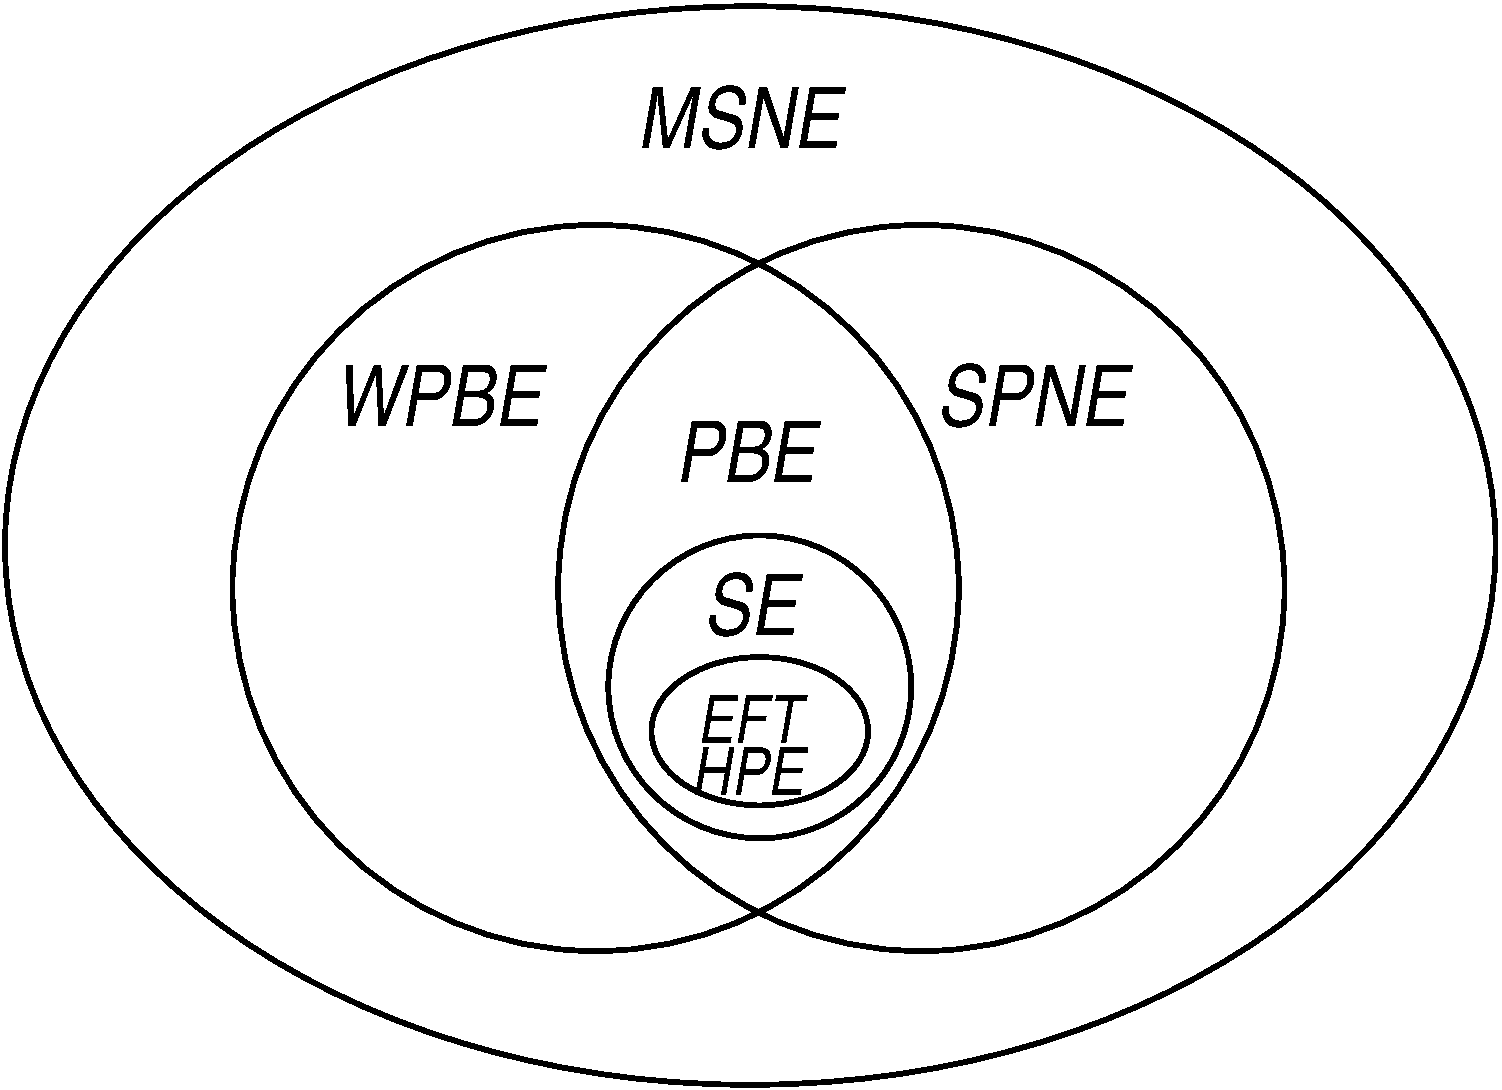
\includegraphics[width=.6\linewidth]{images/equil} \end{center}

\litem{Rationalizable strategy}{Bernheim 27}
\begin{enumerate}
\item A \textit{$ 1 $-rationalizable strategy} is a best response to some (independent)\footnote{Question is whether to allow other players' randomized strategies to be correlated with each other.} probability distribution over other players' strategies.
\item A \textit{$ k $-rationalizable strategy} is a best response to some (independent) probability distribution over other players' $ (k-1) $-rationalizable strategies.
\item A \textit{rationalizable strategy} is $ k $-rationalizable for all $ k $.
\end{enumerate}
For two player games, rationalizable strategies are precisely those that survive iterative deletion of dominated strategies. This equivalence holds for games with more than two players only if we do not insist on independence in defining rationalizability; if we \textit{do} insist on independence, the set of rationalizable strategies is smaller.

\litem{Pure strategy Nash equilibrium}{Bernheim 29--33}\index{PSNE (pure strategy Nash equilibrium)} $ s^* \in S $ is a PSNE iff for all $ s \in S $, we have $ g_i (s_i^* , s_{-i}^*) \geq g_i (s_i , s_{-i}^*) $. The strategies played in a PSNE are all rationalizable.

A finite game of perfect information has a PSNE [Zermelo].\index{Zermelo's Theorem} Proved using backwards induction.

If $ S_1 , \dotsc , S_I $ are compact, convex Euclidean sets and $ g_i $ is continuous in $ s $ and quasiconcave in $ s_i $, then there exists a PSNE. By Berge's Theorem, the best response correspondence is upper hemi-continuous. By quasiconcavity of $ g_i $, the best response correspondence is convex valued. Thus by Kakutani's Fixed Point Theorem, it has a fixed point.

\litem{Mixed strategy Nash equilibrium}{Bernheim 56--9}\index{MSNE (mixed strategy Nash equilibrium)} We define a new game where the strategy space is the set of probability distributions over (normal form) strategies in the original game (i.e., the set of \textit{mixed strategies}). A MSNE of the original game is any PSNE of this new game. Players must be indifferent between playing any strategies included (with strictly positive probability) in a MSNE.

Another approach is to consider randomization over actions at each information set (\textit{behavior strategies}). However, Kuhn's Theorem\index{Kuhn's Theorem} assures us that for any game of perfect recall there are mixed strategies that yields the same distribution over outcomes as any combination of behavioral strategies; also it gives that there are behavioral strategies that yield the same distribution over outcomes as any combination of mixed strategies.

Every finite game has a MSNE.

\litem{Trembling-hand perfection}{Bernheim 65--7}\index{THPE (trembling-hand perfect equilibrium)} There is always some risk that another player will make a ``mistake.'' Bernheim notes include two equivalent rigorous definitions; original definitions are for finite games, but there is an extension available for infinite games. Key notes:
\begin{enumerate}
\item In a THPE, no player selects a weakly dominated strategy with positive probability.
\item For two player games, an MSNE is a THPE iff no player selects a weakly dominated strategy with positive probability.
\item For more than two player games, the set of THPE may be smaller than the set of MSNE where no player selects a weakly dominated strategy with positive probability; if we allow correlations between the trembles of different players, the sets are the same.
\end{enumerate}

\litem{Correlated equilibrium}{Bernheim 70}\index{CE (correlated equilibrium)} In a finite game $ (\{ S_i \}_{i=1}^{I}, g) $, a probability distribution $ \delta^* $ over $ S $ is a CE iff for all $  i $ and $ s_i $ chosen with strictly positive probability, $ s_i $ solves
\[ \max_{s_{i}' \in S_i} \E_{s_{-i}} [g_i (s_{i}' , s_{-i}) | s_i , \delta^* ] ; \]
i.e., player $ i $ has no incentive to defect from any strategy $ s_i $, assuming that other players respond per $ \delta^* $.

\litem{Bayesian Nash equilibrium}{Bernheim 73--4}\index{BNE (Bayesian Nash equilibrium)} Per Harsanyi, we write our game of incomplete information as a game of imperfect information where nature selects hidden characteristics. A BNE is a MSNE of this ``Bayesian game.'' A pure strategy BNE is a PSNE of the Bayesian game.

Characterized by a set of decision rules that determine each player's strategy contingent on his type.

\litem{Subgame perfect Nash equilibrium}{Bernheim 92}\index{SPNE (subgame perfect Nash equilibrium)} A MSNE in behavior strategies $ \delta^* $ is a SPNE iff for every proper subgame, the restriction of $ \delta^* $ to the subgame forms a MSNE in behavior strategies.

For finite games, we can find SPNE using backwards induction on subgames of extensive form.

A SPNE need not be a WPBE, and a WPBE need not be a SPNE.

\litem{Sequentially rational strategy}{Bernheim 94} Behavior strategy profile $ \delta $ is sequentially rational given a system of beliefs $ \mu  $ iff for all information sets $ h \in H $, the actions for player $ \phi(h) $ at $ h \cup [\bigcup_{t \in h} S(t)] $ are optimal starting from $ h $ given an initial probability over $ h $ governed by $ \mu $, and given that other players will adhere to $ \delta_{-\phi(h)} $.

\litem{Weak perfect Bayesian equilibrium}{Bernheim 93--5}\index{WPBE (weak perfect Bayesian equilibrium)} Implausible equilibria can still be SPNE, because we lack beliefs at each information set. Behavior strategy profile $ \delta^* $ \textit{and system of beliefs} $ \mu^* $ are a WPBE iff:
\begin{enumerate}
\item $ \delta^* $ is sequentially rational given beliefs $ \mu^* $, and
\item Where possible, $ \mu^* $ is computed from $ \delta^* $ using Bayes' rule; i.e., for any information set $ h $ with $ \Pr (h | \delta^*) > 0 $, for all $ t \in h $,
\[ \mu^* (t) = \frac{\Pr (t | \delta^*)}{\Pr (h | \delta^*) }. \]
\end{enumerate}

Note only restriction on out-of-equilibrium beliefs is that they exist. A SPNE need not be a WPBE, and a WPBE need not be a SPNE.

\litem{Perfect Bayesian equilibrium}{Bernheim 93--5}\index{PBE (perfect Bayesian equilibrium)} $ (\delta^* , \mu^*) $ is a PBE if it a WPBE in all proper subgames. This ensures it is also a SPNE.

\litem{Consistent strategy}{Bernheim 98} Behavior strategy profile $ \delta $ is consistent given a system of beliefs $ \mu $ iff there exists a sequence of strictly mixed behavior strategy profiles $ \delta_n \to \delta $ such that $ \mu_n \to \mu $, where $ \mu_n $ is generated from $ \delta_n $ by Bayes' rule.

\litem{Sequential equilibrium}{Bernheim 98}\index{SE (sequential equilibrium)} $ (\delta^* , \mu^*) $ is a SE if it is sequentially rational  and consistent.

SE places additional restriction on beliefs vs. WPBE, hence $ \text{SE} \subseteq \text{WPBE} $; also, can show that SE are SPNE, so an SE is also a PBE.

\litem{Extensive form trembling hand perfection}{Bernheim 102--5}\index{EFTHPNE (Extensive form trembling hand perfect equilibrium)} ``Agent normal form'' is the normal form that would obtain if each player selected a different agent to make her decisions at every information set, and all of a player's agents acted independently with the object of maximizing the player's payoffs. An EFTHPE is a THPE in the agent normal form of the game.

$ \text{EFTHPE} \subseteq \text{SE} $; for generic finite games, they are the same.

\subsection{Basic game-theoretic models}
Other models and examples are throughout Bernheim lecture notes.

\litem{Cournot competition}{Bernheim 11, 46--50} Firms simultaneously choose quantity. Inverse demand is $ P(Q) $ (monotonically decreasing); cost to firm $ i $ of producing quantity $ q_i $ is $ c_i (q_i) $ where $ c_i (0) = 0 $. Normal form:
\begin{enumerate}
\item Strategies: $ S = \R_{+}^{I} $;
\item Payouts: $ g_i (s) = P(\sum_j s_j) s_i - c_i (s_i) $.
\end{enumerate}

To ensure PSNE existence, we need quasiconcavity of $ g_i $ in $ s_i $ (generally don't worry about unboundedness of strategy set). Sufficient conditions are $ c_i (\cdot) $ convex and $ P (\cdot) $ concave. The former rules out increasing returns to scale. The latter ``is not a conventional property of demand functions, but \textit{is} satisfied for linear functions.''

Note:
\begin{enumerate}
\item Characterized by strategic substitutes; i.e., best response curves are downward sloping.
\item Production is spread among firms.
\end{enumerate}

\litem{Bertrand competition}{Bernheim 11, 37} Firms simultaneously choose price; consumers purchase from low-price firm. Demand is $ Q(p) $ (monotonically decreasing); cost to firm $ i $ of producing quantity $ q_i $ is $ c_i (q_i) $ where $ c_i (0) = 0 $. Normal form (two-firm case):
\begin{enumerate}
\item Strategies: $ S = \R_{+}^{I} $;
\item Payouts:
$$ g_i (s) = \begin{cases}
0, & s_i > s_{-i}; \\
s_i Q(s_i) - c_i (Q(s_i)), & s_i < s_{-i}; \\
\tfrac{1}{2} \bigl [s_i Q(s_i) - c_i (Q(s_i)) \bigr ], & s_i = s_{-i} .
\end{cases}
$$
\end{enumerate}
Note:
\begin{enumerate}
\item One firm case is monopoly (in which case demand matters); more than one yields perfectly competitive outcome since only the marginal cost of the second-most efficient firm matters---the properties of the demand curve are then irrelevant.
\item Characterized by strategic complements; i.e., best response curves are upward sloping.
\item All production is done by most efficient firm.
\end{enumerate}

\litem{Bertrand competition---non-spatial differentiation}{Bernheim 38--40} Firm $ i $ chooses price for good $ i $. Demand for good $ i $ is given by $ Q(p_{i}, p_{-1}) $. Strategic complements; i.e., best response curves are upward sloping.

\litem{Bertrand competition---horizontal differentiation}{Bernheim 40--2} a.k.a.\ Hotelling spatial location model\index{Hotelling spatial location model}. Consumers are indexed by $ \theta \in [0,1] $, representing location. Each consumer purchases zero or one unit, with payoff $ 0 $ if no purchase, and $ v - p_i - t (x_i - \theta)^2 $ from purchasing a type $ x_i $ good at price $ p_i $. $ v $ is value of good, $ t $ is unit transport cost.

If firms cannot choose product type $ x_i $, prices are strategic complements; i.e., best response curves are upward sloping.

\litem{Bertrand competition---vertical differentiation}{Bernheim 42--5} Consumers are indexed by $ \theta \in [0,1] $, representing value attached to quantity. Each consumer purchases zero or one unit, with payoff $ 0 $ if no purchase, and $ \theta v_i - p_i $ from purchasing a quality $ x_i $ good at price $ p_i $.

\litem{Sequential competition}{Bernheim 107--12} First one firm selects price/quantity, then the other firm follows. The leader always does (weakly) better than in the simultaneous choice model; whether the follower does better or worse than in simultaneous choice depends whether there are strategic complements or substitutes. This also determines which firm does better in the sequential choice model.

\litem{Herfindahl-Hirshman index}{Bernheim 37} $ \mathcal{H} \equiv 10000 \times \sum_i \alpha_i^2 $, where $ \alpha_i $ is the market share of firm $ i $. When all $ N $ firms evenly split market, $ \mathcal{H} = 10000 / N $.

\litem{Lerner index}{Bernheim 37} $ \mathcal{L} \equiv \sum_i \alpha_i \mathcal{L}_i $, where $ \mathcal{L}_i \equiv \frac{p_i - c'_i (q_i)}{p_i} $ is firm $ i $'s margin and $ \alpha_i $ is the market share of firm $ i $.

\litem{Monopolistic competition}{Bernheim 135--8}
\begin{enumerate}
\item Products are distinct, and each firm faces a downward-sloping demand curve;
\item The decisions of any given firm have negligible effects on any other firm (note this does \textit{not} hold for the Hotelling model, where firms have a measurable effect on their neighbors);
\item There is free entry, with zero profits.
\end{enumerate}
Can formalize as a vector of $ N $ differentiated commodities (for $ N $ large) and a numeraire good $ y $, where representative consumer has utility
\[ u(x, y) = y + g \Bigl(  \sum_{i=1}^{N} f(x_i) \Bigr) \]
and the curvature of $ f(\cdot) $ gives the extent of substitutability of the goods.

Relationship between equilibrium variety and optimal variety is dictated by:
\begin{enumerate}
\item When a product is added, revenues generated fall short of incremental consumer surplus because firms can't perfectly price discriminate; this biases towards too little entry.
\item Firms don't take into account the effect of introducing a product on the profits of others; if goods are substitutes, this biases towards too much entry.
\end{enumerate}
If goods are complements, these biases reinforce and we have too little variety relative to social optimum.

\litem{Entry deterrence}{Bernheim } An incumbent can take some action with long-term commitment prior to the arrival of an entrant that makes entry less attractive. For example:
\begin{enumerate}
\item Selecting to produce a middle-of-the-road product (Hotelling model); note the deterrent action is the same as what the firm would do if it faced no entry with certainty (entry is ``blockaded.'')
\item Producing a proliferating range of products (e.g., RTE cereal).
\item Preemptive investment in production capacity; shifts a portion of marginal cost to a sunk cost. Note entrant may also limit capacity to reduce threat to incumbent.
\end{enumerate}

\litem{Vickrey auction}{Bernheim 22--3, 82--3} a.k.a.\ second-price auction\index{Second-price auction}. $ I $ bidders simultaneously submit sealed bids for an item that each values at $ v_i $. Winning bidder pays second highest bid. Bidding $ p_i = v_i $ weakly dominates any other pure strategy, and is not weakly dominated by any other strategy. Analysis does not depend on complete vs. incomplete information---everyone bidding their valuation is a BNE.

\litem{First-price sealed bid auction}{Bernheim 83--7} $ I $ bidders simultaneously submit sealed bids for an item that each values at $ v_i $. Winning bidder pays his own bid. Symmetric BNE gives a decision rule where each bids below his valuation.

Realized revenues typically differ from Vickrey (second-price sealed bid) auction, but expected revenue is the same \textit{given independent private valuations} (per the revenue equivalence theorem\index{Revenue equivalence theorem}).

\litem{English auction}{Bernheim 87} a.k.a.\ ascending price auction\index{Ascending price auction} Posted price of good is slowly increased until only one bidder remains. Staying in until posted price exceeds valuation is a weakly dominated strategy; outcomes are equivalent to Vickrey (second-price sealed bid) auction.

\litem{Dutch auction}{Bernheim 87} a.k.a.\ descending price auction\index{Descending price auction} Posted price of good is slowly decreased until a bidder buys. Outcomes are equivalent to first-price sealed bid auction.

\litem{Public good}{Bernheim 51--4} A non-rival and non-excludable good.

\litem{Spence signaling model}{Bernheim 218--35}\index{Signaling} Workers choose education level; education does nothing for worker's productivity, but is less costly on margin for more productive workers. All workers have same outside opportunities. Three types of WPBE:
\begin{enumerate}
\item Separating equilibria: different types choose different education levels.
\item Pooling equilibria: different types choose same education levels. (Note pooling equilibria with strictly positive levels of education are highly inefficient---education adds nothing to productivity nor does it differentiate workers.)
\item Hyprids: some members of differently-typed groups pool, others separate.
\end{enumerate}
Equilibrium satisfies equilibrium dominance condition\index{Equilibrium dominance} a.k.a.\ the ``intuitive criterion'' iff whenever an individual gets some level of education that no one should in equilbrium, no low-productivity worker should ever choose, and some high-productivity worker could conceivably choose, the firm assumes he is a high-productivity worker with certainty.

\subsection{Repeated games with complete information}
\litem{Infinitely repeated game}{Bernheim 164--5} A \textit{supergame}\index{Supergame} formed by (potentially) infinite repetitions of some \textit{stage game}\index{Stage game} (i.e., the game played in each period). Note there need not actually be infinite repetitions, but there must be a nonzero possibility in each stage that the game will continue.

Given absence of terminal nodes, need mapping from strategies to expected payoffs, e.g.,
\begin{enumerate}
\item Discounted payoffs: $ u_i (v_i) = \sum_{t=0}^{\infty} \delta^{t} v_i (t) $, where the discount factor may reflect both time preference and the probability of continuation.
\item Average payoffs: $ u_i (v_i) = \lim_{T \to \infty} \tfrac{1}{T} \sum_{t=1}^{T} v_i (t) $.
\item Overtaking criterion\index{Overtaking criterion}: a strategy is preferred iff there is some $ T $ beyond which all partial sums of stage game payoffs exceed the corresponding partial sum for other strategies; n.b., only a partial ordering.
\end{enumerate}

\litem{Feasible payoff}{Bernheim 169--70} The convex hull of payoff vectors from pure strategy profiles in the stage game. Note this is potentially larger than the set of payoffs achievable through mixed strategies, since we allow for correlations.

\litem{Individually rational payoff}{Bernheim 170--1} (Stage game) payoff vectors where each player receives at least his minmax payoff
\[ \pi_{i}^{m} \equiv \min_{\delta_{-i}} \max_{\delta_{i}} \pi_{i} (\delta). \]

\litem{Folk Theorem}{Bernheim 171--2, 5, 7--8} Consider a supergame formed by repeating a finite stage game an infinite number of times; suppose players use the average payoff criterion. Then the set of \textit{feasible} and \textit{individually rational} payoffs is precisely the set of average payoffs for Nash equilibria (which need not be SPNE).
\begin{enumerate}
\item ``Anything can happen;'' this makes comparative statics are problematic.
\item Inability to write binding contracts is not very damaging; anything attainable through a contract can also be obtained through some self-enforcing agreement (if there is no discounting).
\end{enumerate}

For discounted payoffs, all feasible payoffs that strictly exceed minmax payoffs for every player are the average payoff for some NE and all discount rates sufficiently close to 1.

Subject to some technical conditions, versions of the folk theorem (with and without discounting) hold for SPNE.

\litem{Nash reversion}{Bernheim 176--7} a.k.a.\ ``grim trigger'' strategy.\index{Grim trigger strategy@``Grim trigger'' strategy}  Players attempt to support cooperation, reverting to a static (stage-game) equilibrium as punishment if someone deviates. If a Nash reversion strategy is a NE, then it is a SPNE.

\litem{Finitely repeated game}{Bernheim 179--80} If there is a unique (up to payoffs) NE for the stage game, there is a unique SPNE for the repeated game, consisting of the repeated stage game equilibrium. However, cooperation may be possible when the stage game has multiple NE.

\litem{Stick-and-carrot equilibrium}{Bernheim 185--6} If a firm strays from the (cooperative) equilibrium path, all firms \textit{including itself} punish it for one period. If any firm does not participate in the punishment (including the punished firm itself), it gets punished again in the next period. The punishment is the ``stick;'' the fact that punishment will end as soon as the firm punishes itself is the ``carrot.''

\subsection{Collusion and cooperation}
\litem{Core}{Jackson; MWG 653--4} The core is the set of allocations not \textit{blocked} by any coalition. A coalition will block an allocation if there is some allocation feasible for the coalition such that each member is strictly better off (``strong blocking''), or that every member is weakly better off and some member is strictly better off (``weak blocking'').

Core allocations must be Pareto optimal.

The set of Walrasian equilibria is a subset of the core (basically, the FWT) since there are no externalities. In other settings, the core could be empty due to externalities.

\litem{Core convergence}{Jackson; MWG 655--7} As we increase the number of ``replicas'' of a pure exchange economy, the core of the replicated economy converges to (equal treatment replicas of) the W.E. of the original economy.

\litem{Nontransferable utility game}{Jackson}\index{NTU (nontransferable utility) game} Feasible allocations for a coalition $ T $ must be listed explicitly.

\litem{Transferable utility game}{Jackson; MWG 676}\index{TU (transferable utility) game} Feasible allocations for a coalition $ S $ are $ V(S) \equiv \R_+^{\lvert S \rvert} $. Generally assume:
\begin{enumerate}
\item The normalization $ V ( \emptyset ) = 0 $;
\item $ V(I) \geq V(S) + V (I \setminus S) $ for all $ I \subseteq S $, where $ I $ is the set of all players;
\item Superadditivity (a stronger version of the prior assumption): $ V(S \cup T) \geq V(S) + V(T) $ when $ S \cap T = \emptyset $.
\end{enumerate}

In a TU game, an allocation can be strictly blocked iff it can be weakly blocked; the weak and strong cores are therefore identically
$$ \{ x \in R^{\lvert I \rvert} \colon \sum_{i} x_i = V(I) \text{ and } \forall S \subseteq I, \sum_{i} x_i \geq V(S) \} . $$

\litem{Shapley value}{Jackson; MWG 673, 679--81} Given a characteristic function $ V \colon 2^I \to \R_+ $, the Shapley value is value function:
\[ \phi_i^{\text{SV}} (V) \equiv \sum_{S \subseteq I \text{ s.t.~} i \not \in S} \frac{\lvert S \rvert ! \, (\lvert I \rvert - \lvert S \rvert - 1)!}{\lvert I \rvert!} \bigl[ V(S \cup \{ i \}) - V(S) \bigr] . \]
That is, the average marginal value that $ i $ contributes over all possible orderings in which members could be added to a coalition. It is a normative allocation, and can be seen as a positive description under certain kinds of bargaining regimes.

The Shapley value is the unique value function satisfying:
\begin{enumerate}
\item Symmetry: If we relabel agents, the Shapley values are relabeled accordingly.
\item Carrier:\index{Carrier axiom} $ T \subseteq I $ is a carrier iff $ V (S \cap T) = V(S) $ for all $ S \subseteq I $; if $ T $ is a carrier, then $ \sum_{i \in T} \phi_i (V) = V(I) = V(T) $.
\item Dummy:\index{Dummy axiom} $ i $ is a dummy iff $ V(S \cup \{ i \}) = V(S) $ for all $ S \subseteq I $; if $ i $ is a dummy, $ \phi_i (V) = 0 $. Note Carrier $ \implies $ Dummy.
\item Additivity: $ \phi (V + W) = \phi(V) + \phi(W) $; implies that $ \phi (\lambda V) = \lambda \phi (V) $. Convenient, but not mathematically clear why this should hold.
\end{enumerate}

\litem{Simple game}{Jackson} A TU game where
\begin{enumerate}
\item $ V(S) \in \{ 0,1 \} $,
\item $ S \subseteq T \implies V(S) \leq V(T) $,
\item $ V(S) = 1 \implies V(I \setminus S) = 0 $,
\item $ V(I) = 1 $.
\end{enumerate}

In a simple game, $ i $ is a ``veto player''\index{Veto player} iff $ V(S) = 1 \implies i \in S $. The core is nonempty iff there is at least one veto player. Shapley values are then:
\[ \phi_i^{\text{SV}} = \begin{cases}
\tfrac{1}{\text{\# of veto players}}, & i \text{ is a veto player}; \\
0, & \text{otherwise}.
\end{cases} \]
If the set of veto players is a carrier, $ \phi^{\text{SV}} \in \text{core} $.

\litem{Convex game}{Jackson; MWG 683} A TU game $ V (\cdot) $ is convex iff $ S \subseteq T $ and $ i \not \in T $ implies
\[ V(S \cup \{ i \}) - V(S) \leq V(T \cup \{ i \}) - V(T); \]
i.e., there are \textit{increasing} marginal returns as coalitions grow.

For a convex game, the core is nonempty; the Shapley value is in the core.

\litem{One-sided matching}{Jackson} Players are each allocated one object; each player has ordinal preferences over objects. Given strict preferences, we can find the unique (weak) core allocation using the Top Trading Cycles algorithm\index{Top Trading Cycles algorithm}:
\begin{enumerate}
\item Look for cycles among individuals' top choices;
\item Assign each member of cycles her top choice;
\item Return to step 1, with already assigned individuals/objects removed from consideration.
\end{enumerate}

We can support this core as a competitive equilibrium by assigning a common price to the objects in each cycle as they are assigned. The price for cycles assigned in the same round can vary across cycles, but must be strictly lower than the prices for objects assigned in previous rounds.

The algorithm is strategy-proof: truth telling dominates.

\litem{Two-sided matching}{Jackson} Two sets $ M $ and $ W $, which may have different cardinalities. Every individual is either matched to someone in the other set, or remains unmatched.

Can find two core allocations (here strict $ = $ weak) using Gale-Shapley [a.k.a.\ Deferred acceptance] algorithm\index{Gale-Shapley algorithm}\index{GS (Gale-Shapley) algorithm}\index{Deferred acceptance algorithm}: Suppose $ M $ ``propose,'' then
\begin{enumerate}
\item Each $ M $ proposes to his favorite $ W $ to whom he has not yet proposed (unless he would prefer to stay single);
\item Each $ W $ who has been proposed to accepts her favorite proposal (unless she would prefer to stay single)---this could involve breaking an engagement she made in a previous round;
\item Return to step 1, where the only unengaged $ M $ propose (i.e., those who either had a proposal rejected last round, or had an engagement broken).
\end{enumerate}

The core is a lattice; Gale-Shapley algorithm yields ``best'' for proposing group (and ``worst'' for other group). Thus if we get same result from $ M $-proposing and $ W $-proposing algorithms, core is a singleton. Note this result relies on:
\begin{itemize}
\item Two-sided matching (cf, roommate matching);
\item One-to-one matching (cf, firm and workers);
\item Strict preferences.
\end{itemize}

The algorithm is \textit{not} strategy-proof: there may be profitable manipulations (lying by rejecting proposals), but they are typically difficult to implement.

\subsection{Principal-agent problems}
\litem{Moral hazard}{Jackson} ``Hidden action'' problems. Agent takes (non-contractable) action $ e $, outcome $ \pi $ has some distribution that varies based on $ e $. Generally assume risk-neutral principal and risk-averse (and/or liability-limited) agent, so that optimal solution is not merely ``selling the firm to the agent.''

Principal structures optimal contract---payment $ w(\pi) $ as a function of realized outcome---that, for a desired effort level $ e^* $,
\begin{enumerate}
\item Maximizes principal's expected payoff: $ \E [\pi - w(\pi) | e^*] $;
\item Satisfies the agent's participation constraint (i.e., individual rationality constraint): $ \E [u(w(\pi)) | e^* ] - g(e^*) \geq \bar{u} $, where $ g(\cdot) $ is the agent's cost of effort, and $ \bar{u} $ is his reservation utility;
\item Satisfies the agent's incentive compatibility constraint: $ e^* \in \argmax_{e} \E [u(w(\pi)) | e ] - g(e) $.
\end{enumerate}

\litem{Adverse selection}{Jackson}  ``Hidden information'' problems. Can be mitigated using, e.g., warantees, repeated interaction, reputation mechanisms, signaling/screening.

\litem{Signaling}{Jackson}\index{Spence signaling model} Agents choose a costly signal (which per Spence is often assumed to be meaningless other than for its informational value), and then principals Bertrand bid for contracts with agents.

A multitude of pure strategy sequential equilibria typically exist---both pooling (various types choose same signal) and separating (various types choose different signals).

\litem{Screening}{Jackson} Bertrand principals announce a schedule of contracts they are willing to engage in (pairs of signals and wages), and then agents choose a contract (and hence a signal).

No pooling equilibria can exist, and there is only one separating equilibrium that can exist (but may not). Thus in contrast with signaling, where our problem was a multitude of PSNE, screening games may have no PSNE.

\subsection{Social choice theory}
\litem{Voting rule}{Jackson} $ n $ individuals must choose among a set $ A $ of alternatives. Each individual has a complete, transitive preference relation $ \succ_i $ over $ A $ that does not have indifference.

A voting rule $ R (\succ) \equiv R (\succ_1, \dotsc , \succ_n) $ gives a social welfare ordering over $ A $ (which in general allows indifference). The corresponding strict social welfare ranking is $ P (\succ) $.

\litem{Neutrality}{Jackson} For $ A = \{ a , b \} $ (i.e., $ |A| = 2 $), consider $ \succ $ and $ \succ' $ with $ \succ_i \neq \succ'_i $. Then $ R(\cdot) $ is neutral (over alternatives) iff $ a R(\succ) b \iff b R (\succ') a $.

\litem{Anonymity}{Jackson} Let $ \pi (\cdot) $ be a permutation over $ \{ 1 , \dotsc , n \} $. Define $ \succ'_i \equiv \succ_{\pi(i)}  $. Then $ R(\cdot) $ is anonymous (over individuals) iff $ a R(\succ) b \iff a R (\succ') b $.

\litem{Monotonicity}{Jackson} Consider $ \succ $ and $ \succ' $ with $ \succ_j = \succ'_j $ for all $ j \neq i $, and $ \succ_i = a $ while $ \succ'_i = b $. Then $ R(\cdot) $ satisfies monotonicity iff $ b R(\succ) a \implies b R(\succ') a $.

$ R(\cdot) $ satisfies strict monotonicity iff $ b R(\succ) a \implies b P(\succ') a $.

\litem{May's Theorem}{Jackson} Let $ A = \{ a , b \} $ (i.e., $ |A| = 2 $). Then $ R(\cdot) $ is complete, transitive (which has no bite for $ |A| = 2 $), neutral, anonymous, and satisfies \textit{strict} monotonicity iff it is majority rule.

If we replace strict monotonicity with monotonicity, we get that $ R(\cdot) $ must be a quota rule.

\litem{Unanimity}{Jackson} $ \R( \cdot) $ is unanimous iff $ a \succ_i b \forall i $ implies that $ a P(\succ) b $.

\litem{Arrow's independence of irrelevant alternatives}{Jackson}\index{AIIA (Arrow's independence of irrelevant alternatives)} Consider $ \succ $ and $ \succ' $ with $ a \succ_i b \iff a \succ'_i b $ for all $ i $.

$ \R( \cdot) $ satisfies AIIA iff $ a R(\succ) b \iff a R(\succ') b $; i.e., $ R(\succ) $ over $ \{ a, b \} $ only depends on $ \succ $ over $ \{ a, b \} $, not over any other (``irrelevant'') alternatives.

\litem{Arrow's Theorem}{Jackson; Micro P.S.~4} Let $ |A| \geq 3 $. Then $ R(\cdot) $ is complete, transitive, unanimous, and satisfies AIIA iff it is dictatorial (i.e., if there is some $ i $ such that $ \forall \succ $, $ a P(\succ) b \iff a \succ_i b $).

The theorem is tight; i.e., giving up any of completeness, transitivity, unanimity, or AIIA allows a non-dictatorial $ R(\cdot) $.

\litem{Condorcet winner}{Jackson} $ a \in A $ is a Condorcet winner iff it is majority preferred to every other alternative.

\litem{Condorcet-consistent rule}{Jackson} A voting rule that picks the Condorcet winner if there is one.

\litem{Gibbard-Satterthwaite Theorem}{Jackson}\index{GS (Gibbard-Satterthwaite) Theorem} Let $ 3 \leq |A| < \infty $, and $ F (\cdot) $ be a social choice function (note we do not require a full ordering). Then $ F ( \cdot ) $ has range $ A $ (implied by unanimity) and is strategy-proof (i.e., DSIC) iff it is dictatorial.

\litem{Vickrey-Clarke-Groves mechanism}{Jackson}\index{VCG (Vickrey-Clarke-Groves) mechanism}\index{Groves mechanism} Let $ \theta_i \in \Theta_i $ be the type of individual $ i $, and $ \hat{\theta}_i $ be his announced type. Suppose $ d(\theta) $ makes ex post efficient decisions. Then a mechanism with transfers
\[ t_i (\hat{\theta}) = \sum_{j \neq i} \bigl [ u_j (d(\hat{\theta}), \hat{\theta}_j) \bigr ] + x_i (\hat{\theta}_{-i}) \]
for any $ x_i (\cdot) $ is dominant-strategy incentive compatible (DSIC).

Conversely, if $ (d, t) $ is DSIC, $ d(\cdot) $ is ex post efficient, and $ \Theta_i $ is sufficiently rich such that $ \forall v_i \in \{v_i \colon D \to \R \} $ there exists $ \theta_i $ such that $ v_i (\cdot) = u_i (\cdot , \theta_i) $, then $ t (\cdot) $ must satisfy the above condition.

Note that Gibbard-Satterthwaite says that a general DSIC mechanism must be dictatorial. However, here we have restricted ourselves to quasilinear preferences, and get a DSIC mechanism without being dictatorial. However, although it reaches an efficient decision it is \textit{not} always balanced (payments do not total to zero), and hence is not typically overall efficient.

\litem{Pivotal mechanism}{Jackson} An example of a VCG mechanism where
\[ t_i (\hat{\theta}) = \sum_{j \neq i} \bigl [ u_j (d(\hat{\theta}), \hat{\theta}_j) \bigr ] - \max_{d} \sum_{j \neq i} u_j (d, \hat{\theta}_j) . \]
That is, the transfers are the externality imposed on others by choosing $ d ( \hat{\theta} ) $ instead of $ d ( \hat{\theta}_{-i} ) $.

Ensures feasibility, since transfers are always negative. However, budget generally doesn't balance---there is a need to ``burn money.''

\hrule
\section{Macroeconomics}
\subsection{Models}
\litem{Two period intertemporal choice model}{Nir 1-11} Maximize $ U(C_0, C_1) $ subject to $ C_0 + S_0 \leq Y_0 $ and $ C_1 \leq R S_0 $. The constraints can be rewritten $ C_0 + \tfrac{1}{R} C_1 \leq Y_0 $.

\litem{Neoclassical growth model (discrete time)}{Nir 3-3--5, 11-3, 8, 10, 16--28, 12-12--26}\index{NCGM (neoclassical growth model)} (a.k.a.\ Ramsey model\index{Ramsey model}) Maximize $ \sum_{t} \beta^t U(c_t) $ subject to:
\begin{enumerate}
\item $ c_t + k_{t+1} \leq F(k_t, n_t) + (1- \delta) k_t  $ for all $ t $ (RHS can be denoted $ f(k_t, n) $, or $ f(k_t) $, since the lack of disutility of working ensures that $ n_t=1 $);
\item $ k_{t+1} \geq 0 $ for all $ t $;
\item $ c_t \geq 0 $ for all $ t $;
\item $ k_0 $ is given.
\end{enumerate}
We further assume $ U (\cdot) $ satisfies Inada conditions; that the production function is constant returns to scale and satisfies $ F_{k}' > 0 $, $ F_{kk}'' < 0 $, $ F_{n}' > 0 $, and $ F_{nn}'' < 0 $; and TVC $ \lim_{t \to \infty} \beta^t U'(c_t) f'(k_t) k_t = 0 $.

The problem can be rewritten in ``SL canonical form'' as maximizing $ \sum_{t} \beta^t U(f(k_t) - k_{t+1}) $ subject to $ k_{t+1} \in [0, f(k_t)] $, the given $ k_0 $, and conditions on $ f(\cdot) $ and $ U(\cdot) $ as above. In functional equation form, we write $ V(k) \equiv \max_{k' \in [0, f(k)]} U(f(k) - k') + \beta V(k') $ (again, with additional conditions as above).

Steady state satisfies $ \beta f' (k^*) = 1 $. Note the utility function does \textit{not} affect the steady state (although it will affect dynamics).

Linearization of the intereuler
\[ u'(f(k_t) - k_{t+1}) - \beta f' (k_{t+1}) u' (f(k_{t+1}) - k_{t+2}) = 0 \]
about steady state gives:
$$
\begin{bmatrix}
k_{t+2} - k_* \\
k_{t+1} - k_*
\end{bmatrix}
\approx
\begin{bmatrix}
1 + \frac{1}{\beta} + \beta \frac{U'(c_*)}{U''(c_*)} f''(k_*) & -\frac{1}{\beta} \\
1 & 0
\end{bmatrix}
\begin{bmatrix}
k_{t+1} - k_* \\
k_{t} - k_*
\end{bmatrix}
 $$

The optimal policy function $ g(k) $ satisfies:
\begin{enumerate}
\item $ g(\cdot) $ is single-valued, since the value function is strictly concave.
\item $ g(0) = 0 $ since that is the only feasible choice.
\item $ g(k) $ is in the interior of $ \gamma(k) $, since otherwise exactly one of $ U'(c) $ and $ U'(c') $ would be infinite, violating the Intereuler condition.
\item $ g'(k) > 0 $, since as $ k $ increases, marginal cost of saving goes down, while marginal benefit stays same.
\item There is unique $ k^* >0$ such that $ g(k^*) = k^* $.
\item $ k > k^* \implies k > g(k) > k^* $, and $ k < k^* \implies k < g(k) < k^* $; i.e., capital moves closer to (without crossing over) the steady-state level.
\item The sequence $ k_0, g(k_0), g(g(k_0)), \dotsc $ displays monotonic and global convergence.
\end{enumerate}

\litem{Endowment economy, Arrow-Debreu}{Nir 13-4--6} At every period household gets $ y_t $ units of good; there is no storage, and trading in all commodities (goods delivered in each period) takes place in period $ 0 $. Maximize $ \sum \beta^t U(c_t) $ subject to $ \sum p_t c_t \leq \sum p_t y_t $ (budget constraint), and ensure $ y_t = c_t $ (market clearing).

\litem{Endowment economy, sequential markets}{Nir 13-7--9} At every period household gets $ y_t $ units of good; there is no storage, and trading in ``assets'' (loans across periods) takes place each period. Maximize $ \sum \beta^t U(c_t) $ subject to $ c_t + a_{t+1} \leq y_t + R_t a_t $ (budget constraint), and ensure $ y_t = c_t $, $ a_{t+1} = 0 $ (market clearing).

\litem{Production economy, Arrow-Debreu}{Nir 13-10--6} Household owns capital rented for production by competitive firms, which also rent labor from households. Capital depreciates at rate $ \delta $. There is no storage, and trading in all commodities (goods delivered, capital rental, and labor in each period) takes place in period $ 0 $.
\begin{enumerate}
\item Households maximize $ \sum \beta^t U(c_t) $ subject to $ \sum p_t [c_t + k_{t+1}] \leq \sum p_t [r_t k_t + (1-\delta) k_t + n_t w_t] $.
\item Firms maximize (in each period) $ p_t F(k_t, n_t) - p_t r_t k_t - p_t w_t n_t $.
\item Markets clear: $ c_t + k_{t+1} = F(k_t, n_t) + (1-\delta) k_t $.
\end{enumerate}
Note the rental rate of capital ($ r_t $) and wage rate ($ w_t $) are measured in units of consumption good.

\litem{Production economy, sequential markets}{Nir 13-25} As above, household owns capital rented for production by competitive firms, which also rent labor from households. Capital depreciates at rate $ \delta $. There is no storage, and each period, goods delivered, capital rental, and labor are traded. Note there is no inter-period trading, so we do not need a price for goods.
\begin{enumerate}
\item Households maximize $ \sum \beta^t U(c_t) $ subject to $ c_t + k_{t+1} \leq r_t k_t + (1-\delta) k_t + n_t w_t $.
\item Firms maximize (in each period) $ F(k_t, n_t) - r_t k_t - w_t n_t $.
\item Markets clear: $ c_t + k_{t+1} = F(k_t, n_t) + (1-\delta) k_t $.
\end{enumerate}

Formulated recursively (assuming $ n=1 $),
\begin{enumerate}
\item Households have $ V(k, K) = \max_{c, k'} [U(c) + \beta V(k', K') $ subject to $ c + k' = R(K) k + W(K) $; where $ K $ is aggregate capital, and $ R(K) $ and $ W(K) $ are the rental and wage rates as functions of aggregate capital. We further require the ``forecast'' of future capital to be rational: $ K' = G(K) $, where $ G (\cdot) $ is the optimal aggregate policy function.
\item Firms maximize $ F(K) - R K - W $, which gives FOC $ R(K) = F_k(K) + 1- \delta $ and $ W(K) = F_n(K) $.
\item Markets clear: $ C + K' = F(K) + (1-\delta) K $.
\item Consistency: $ G(K) = g(K, K) $.
\end{enumerate}

\litem{Overlapping generations}{Nir 17-15--6, 17-32}\index{OLG (overlapping generations)} In an endowment OLG economy, a competitive equilibrium is Pareto optimal iff $ \sum_{t=0}^{\infty} 1 / p_t = \infty $ where the interest rate is $ R_t = p_t / p_{t+1} $.

In an an OLG economy with production, a competitive equilibrium is dynamic efficient iff $ F_{K}' (K_*) + 1 - \delta \geq 1 $.

\litem{Real Business Cycles model}{Nir 18-7--14}\index{RBC (Real Business Cycles) model} Benchmark RBC model is NCGM with endogenous hours, ownership of firms and capital by households, and stochastic productivity $ A_t $ multiplying labor (so production function is $ F(k_t, A_t n_t) $). We specified:
\begin{enumerate}
\item CRRA utility: $ U(c,n) = \frac{c^{1 - \sigma} - 1}{1 - \sigma} - \frac{n^{1 + \chi}}{1 + \chi} $;
\item Cobb-Douglas production: $ y_t = A_t k_t^{\alpha} n_t^{1 - \alpha} $;
\item Productivity given by $ \ln A_t = \rho \ln A_{t-1} + \epsilon_t $ with $ \epsilon_t $ distributed iid normal.
\end{enumerate}

\litem{Optimal taxation---primal approach}{Nir 10}\index{Primal approach to optimal taxation} Solve HH problem and combine FOC and budget constraint with government budget constraint to get one expression that ties together allocations but has \textit{no prices or taxes}. Then goverment maximizes HH utility over \textit{allocations} subject to this constraint.

Note that in the case with capital,\footnote{We generally need to impose restrictions on first-period taxation, since otherwise the government will tax capital very highly then (since it's supplied perfectly inelastically).} the problem is not stationary; i.e., we cannot use our typical dynamic programming tools, and need to worry about the government's ability to commit to a future tax policy.

\subsection{Imperfect competition}
\litem{Imperfect competition model}{Nir 21} Consider two stages of production: final good manufacturer operates competitively, purchasing inputs from intermediate good producers, who are small enough to take general price levels and aggregate demand as given, but whose products are imperfect substitutes to the production process.

\litem{Imperfect competition: final goods}{Nir 21} Final good producer has Dixit-Stiglitz\index{Dixit-Stiglitz aggregator} production technology:
$$ Y = \left[ \int_0^1 Q_j^{\rho} \, dj \right]^{1 / \rho} $$
which is constant elasticity of substitution ($ \frac{1}{1 - \rho} $ between all pairs of inputs) and constant returns to scale. $ \rho \in (0,1) $, with $ \rho \to 1 $ corresponding to a competitive market where all inputs are perfect substitutes.

Conditional factor demands are therefore
$$ Q_j (Y) = \left[ \frac{p_j}{\lambda} \right]^{\frac{1}{\rho - 1}} Y = \left[ \frac{p_j}{P} \right]^{\frac{1}{\rho - 1}} Y, $$
where the Lagrange multiplier on $ [ \int_0^1 Q_j^{\rho} \, dj ]^{1 / \rho} \geq Y $ also satisfies $ \lambda = E^* / Y \equiv P $, the (aggregate) average cost. Solving for this gives
$$ \lambda = P = \left[ \int_0^1 p_j^{\frac{\rho}{\rho - 1}}  \right]^{\frac{\rho - 1}{\rho}}. $$
The own-price elasticity of demand is $ \eta \equiv \frac{1}{\rho - 1} $, ignoring the effects through $ P $.

\litem{Imperfect competition: intermediate goods}{Nir 21} Intermediate goods producers have identical production technologies (affected by same shocks): $ Q_j = z k_j^{\alpha} n_j^{1 - \alpha} - \phi $, where $ \phi > 0 $ is overhead cost (since there aren't really economic profits). Has constant marginal cost, and therefore increasing returns to scale (because of $ \phi $).

Monopolistic problem is to maximize over prices $ p Q(p) - c(Q(p)) $; first-order condition gives $ \operatorname{markup} \equiv p / \operatorname{MC} = \frac{\eta}{1 + \eta} = \frac{1}{\rho} $.

\subsection{General concepts}
\litem{Cobb-Douglas production function}{Macro P.S. 1} $ F(K, N) = z K^\alpha N^{1-\alpha} $. Constant returns to scale. Fraction $ \alpha $ of output goes to capital, and $ 1 - \alpha $ to labor.

\litem{Constant relative risk aversion utility function}{Nir 14-15, 18-72--4}\index{CRRA (constant relative risk aversion) utility function} $ U(c) = (c^{1 - \sigma} - 1) / (1 - \sigma) $, with $ \sigma > 0 $ (reduced to log utility with $ \sigma = 1 $;\footnote{Note the Taylor approximation of $ c^{1 - \sigma} - 1 $ about $ \sigma = 1 $ is $ c^{1 - \sigma} - 1 \approx (c^0 - 1) - c^{0} (\log c) (\sigma - 1) = (1 - \sigma) \ln c  $. Thus as $ \sigma \to 1 $, we have $ U(c) = (c^{1 - \sigma} - 1) / (1 - \sigma) \approx \ln c $.} empirically we expect $ \sigma \in [1,5] $). Relative risk aversion is $ \sigma $. Higher risk aversion also corresponds to a higher desire to smooth consumption over time.

\litem{Additively separability with stationary discounting}{Nir 1-24} General assumption that $ U(C_0, C_1) = u(C_0) + \beta u(C_1) $ with $ \beta \in (0,1) $.

\litem{Intertemporal Euler equation}{Nir 1-28, 11-5}\index{Intereuler equation} $ u'(c_t) = \beta R u'(c_{t+1}) $, where $ R $ is the return on not-consuming (e.g., $ f'(k_{t+1}) \equiv F_{k}' (k_{t+1}, n_{t+1}) + (1 - \delta) $). This first-order difference equation is given by FOCs of the maximization problem for two consecutive time periods.

\litem{Intertemporal elasticity of substitution}{Nir 1-31, Max notes}\index{Elasticity of intertemporal substitution}\index{IEoS (intertemporal elasticity of substitution)} $ - d \ln \tfrac{C_0}{C_1} / d \ln R = - d \ln \tfrac{C_0}{C_1} / d \ln \frac{U'(C_0)}{U'(C_1)} $.

For CRRA utility function $ U(c) = c^{1 - \sigma} / (1 - \sigma) $, intereuler is $ C_0^{-\sigma} = \beta C_1^{-\sigma} R $ so $ \operatorname{IEoS} = \frac{1}{\sigma} = \operatorname{RRA}^{-1} $.

\litem{General equilibrium}{Nir 2-11} A competitive equilibrium is a set of \textit{allocations} and \textit{prices} such that
\begin{enumerate}
\item Actors (i.e., households, firms, \ldots) maximize their objectives;
\item Markets clear; and
\item Resource constraints are satisfied.
\end{enumerate}

\litem{Inada conditions}{Nir 3-5} We generally assume utility satisfies Inada conditions, which imply that the nonnegativity constraint on consumption will not bind:
\begin{enumerate}
\item $ U(0) = 0 $;
\item $ U $ is continuously differentiable;
\item $ U'(x) > 0 $ ($ U $ is strictly increasing);
\item $ U''(x) \leq 0 $ ($ U $ is strictly concave);
\item $ \lim_{x \to 0+} U'(x) = \infty $;
\item $ \lim_{x \to \infty} U'(x) = 0 $.
\end{enumerate}

\litem{Transversality condition}{Macro P.S. 2}\index{TVC (transversality condition)} In NCGM, $ \lim_{t \to \infty} \beta^t U'(c_t) f'(k_t) k_t = 0 $.

\litem{No Ponzi condition}{Max notes} Credit constraint on agents, which should never bind but suffice to prevent the optimality of a ``doubling'' strategy. For example, $ \forall t $, $ a_t \geq - \bar{k} $ for some $ \bar{k} $.

\litem{Dynamic systems}{Nir 12-4--11, Macro P.S.~5-4} Let the sequence $ \{ x_t \} $ evolve according to $ x_{t+1} = W x_t $. Using eigen decomposition $ W = P \Lambda P^{-1} $, giving the ``decoupled system'' $ P^{-1} x_{t+1} = \Lambda P^{-1} x_t $. Then if $ \tilde{x}_t \equiv P^{-1} x_t $, we have $ \tilde{x}_{ti} = \lambda_i^t \tilde{x}_{0i} $ and hence $ x_t = P \Lambda^t \tilde{X}_0 $.

For $ 2 \times 2 $ case, if
\begin{enumerate}
\item $ | \lambda_1 | > 1 $ and $ | \lambda_2 | > 1 $, then the system ``explodes'' unless $ \tilde{x}_{0,1} = \tilde{x}_{0,2} = 0 $ (source).
\item $ | \lambda_1 | < 1 $ and $ | \lambda_2 | < 1 $, then the system converges for any $ \tilde{x}_{0,1} $ and $ \tilde{x}_{0,2} $ (sink).
\item $ | \lambda_1 | < 1 $ and $ | \lambda_2 | > 1 $, then the system converges for any $ \tilde{x}_{0,1} $ as long as $ \tilde{x}_{0,2} = 0 $ (saddle path).
\end{enumerate}

The speed of convergence for a state variable equals one minus the slope of the optimal policy function ($ 1 - g'(k) $).

\litem{First Welfare Theorem}{Nir 13-27} The competitive equilibrium is Pareto optimal. Then if we know our solution to the social planner problem is the unique Pareto optimal solution, we know it must equal the competitive equilibrium.

\litem{Ramsey equilibrium}{Nir 20-3, final solutions} A Ramsey equilibrium is allocations, prices, and taxes such that:
\begin{enumerate}
\item Households maximize utility subject to their budget constraints, taking prices and taxes as given, and
\item Government maximizes households' utility while financing government expenditures (i.e., meeting its budget constraint).
\end{enumerate}

\subsection{Dynamic programming mathematics}
\litem{Metric space}{Nir 6-3--4} A set $ S $ and a distance function $ \rho \colon S \times S \to \R $ such that:
\begin{enumerate}
\item $ \forall x $, $ y \in S $, $ \rho(x, y) \geq 0 $;
\item $ \forall x $, $ y \in S $, $ \rho(x, y) = 0 \iff x = y $;
%\item $ \forall x \in S $, $ \rho(x,x) = 0 $;
\item $ \forall x $, $ y \in S $, $ \rho(x, y) = \rho (y,x) $;
\item Triangle inequality: $ \forall x $, $ y $, $ z \in S $, $ \rho(x, z) \leq \rho (x,y) +  \rho (y,z) $.
\end{enumerate}

\litem{Normed vector space}{Nir 6-5--6} A vector space $ S $ and a norm $ \lVert \cdot \rVert \colon S \to \R $ such that:
\begin{enumerate}
\item $ \forall x \in S $, $ \lVert x \rVert \geq 0 $;
\item $ \forall x \in S $, $ \lVert x \rVert = 0 \iff x = 0 $;
\item Triangle inequality: $ \forall x $, $ y \in S $, $ \lVert x + y \rVert \leq \lVert x \rVert + \lVert y \rVert $.
\item Scalar multiplication: $ \forall x \in S $, $ \forall \alpha \in \R $, $ \lVert \alpha x \rVert = | \alpha | \, \lVert x \rVert $.
\end{enumerate}
Note any normed vector space induces a metric space with $ \rho (x, y) \equiv \lVert x - y \rVert $.

\litem{Supremum norm ($ \R^n $)}{Nir 6-7--8}\index{Sup norm} $ \lVert \cdot \rVert_{\operatorname{s}} \colon \R^n \to \R $ with $ \lVert x \rVert_{\operatorname{s}} \equiv \sup_{i=1, \dotsc , n} |x^i| $.

\litem{Euclidean norm}{Nir 6-9} $ \lVert \cdot \rVert_{\operatorname{E}} \colon \R^n \to \R $ with
$$ \lVert x \rVert_{\operatorname{E}} \equiv \sqrt[n]{\sum_{i=1}^{n} |x_i|^n} . $$

\litem{Continuous function}{Nir 6-10; Micro math 3} $ f \colon S \to \R $ is continuous at $ x $ iff $ \forall y \in S $ and $ \forall \epsilon > 0 $, there exists $ \delta > 0 $ such that $ \lVert y - x \rVert < \delta \implies |f(y) - f(x)| < \epsilon $.

Equivalently, iff for all sequences $ x_n $ converging to $ x $, the sequence $ f(x_n) $ converges to $ f(x) $.

\litem{Supremum norm (real-valued functions)}{Nir 6-7--8}\index{Sup norm} Let $ \operatorname{C}(X) $ denote the set of bounded, continuous functions from $ X $ to $ \R $. Then $ \lVert \cdot \rVert_{\operatorname{s}} \colon \operatorname{C}(X) \to \R $ with $ \lVert f \rVert_{\operatorname{s}} \equiv \sup_{x \in X} |f(x)| $.

\litem{Convergent sequence}{Nir 7-4} The sequence $ \{ x_i \}_{i=0}^{\infty} $ in $ S $ converges to $ x \in S $ (or equivalently, the  sequence has limit $ x $) iff $ \forall \epsilon > 0 $, there exists $ n $ such that $ i > n \implies \lVert x_i - x \rVert < \epsilon $. In other words, there is a point in the sequence beyond which all elements are arbitrarily close to the limit.

\litem{Cauchy sequence}{Nir 7-9} The sequence $ \{ x_i \}_{i=0}^{\infty} $ in $ S $ is Cauchy iff $ \forall \epsilon > 0 $, there exists $ n $ such that $ i > n $ and $ j > n $ together imply that $ \lVert x_i - x_j \rVert < \epsilon $. In other words, there is a point in the sequence beyond which all elements are arbitrarily close to each other. Every convergent sequence is Cauchy (shown via triangle inequality), but not every Cauchy sequence is convergent.

\litem{Complete metric space}{Nir 7-10--16} A metric space $ (S, \rho) $ is complete iff every Cauchy sequence in $ S $ converges \textit{to some point in} $ S $. Importantly, if $ \operatorname{C}(X) $ is the set of bounded, continuous functions from $ X $ to $ \R $, and $ \lVert \cdot \rVert_{\operatorname{s}} \colon \operatorname{C}(X) \to \R $ is the sup norm, then $ (\operatorname{C}(X), \lVert \cdot \rVert_{\operatorname{s}} $ is a complete metric space.

\litem{Contraction}{Nir 8-3--4} If $ (S, \rho) $ is a metric space, the operator $ T \colon S \to S $ is a contraction of modulus $ \beta \in (0,1) $ iff $ \forall x $, $ y \in S $, we have $ \rho (Tx, Ty) \leq \beta \rho (x,y) $. That is, $ T $ brings any two elements closer together. Every contraction is a continuous mapping.

\litem{Contraction Mapping Theorem}{Nir 8-5}\index{CMT (Contraction Mapping Theorem)}\index{Banach fixed point theorem} [a.k.a.\ Banach fixed point theorem.] If $ T $ is a contraction on a \textit{complete} metric space, then
\begin{enumerate}
\item $ T $ has exactly one fixed point $ V^* $ such that $ TV^* = V^* $; and
\item The sequence $ \{ V_i \} $ where $ V_{i+1} = TV_i $ converges to $ V^* $ from any starting $ V_0 $.
\end{enumerate}

\litem{Contraction on subsets}{Nir 8-11} Suppose $ T $ is a contraction on a complete metric space $ (S, \rho) $, with fixed point $ V^* = TV^* $. Further suppose $ Y \subseteq S $ is a closed set, that $ Z \subseteq Y $, and that $ \forall y \in Y $, $ Ty \in Z $. Then $ V^* \in Z $.

\litem{Blackwell's sufficient conditions for a contraction}{Nir 8-12--3} Blackwell gives sufficient (not necessary) conditions for an operator to be a contraction on the metric space $ B(\R^n , \R) $ (the set of bounded functions $ \R^n \to \R $) with the sup norm. An operator $ T $ is a contraction if it satisfies
\begin{enumerate}
\item Monotonicity: if $ \forall x $, $ f(x) \leq g(x) $, then $ \forall x $, $ Tf(x) \leq Tg(x) $; and
\item Discounting: there exists $ \beta \in (0,1) $ such that for all $ \alpha \geq 0 $, $ f (\cdot) $, and $ x $, we have $ T(f(x) + \alpha) \leq T(f(x)) + \beta \alpha $ [slight abuse of notation].
\end{enumerate}

\litem{Principle of Optimality}{Nir 9} Under certain conditions, the solutions to the following two problems are the same:
\begin{enumerate}
\item Sequence problem: $ W(x_0) = \max_{ \{ x_{t+1} \} } \sum_{t=0}^{\infty} \beta^t F(x_t, x_{t+1}) $ such that $ x_0 $ given and $ \forall t $, $ x_{t+1} \in \Gamma (x_t) $.
\item Functional equation: $ V(x) = \max_{x' \in \Gamma (x)} [F(x,x') + \beta V(x')] $.
\end{enumerate}
Assume
\begin{enumerate}
\item \label{assump1} $ \Gamma (x) $ is nonempty for all $ x $;
\item \label{assump2} For all initial conditions $ x_0 $ and feasible plans $ \{ x_t \} $, the limit $ u(\{ x_t \}) \equiv  \lim_{n \to \infty} \beta^t F(x_t, x_{t+1}) $ exists (although it may be $ \pm \infty $).
\end{enumerate}
Then:
\begin{enumerate}
\item If $ W(x_0) $ is the supremum over feasible $ \{ x_t \} $ of $ u( \{ x_t \} ) $, then $ W $ satisfies the FE.
\item Any solution $ V $ to the FE that satisfies boundedness condition $ \lim_{n \to \infty} \beta^n V(x_n) = 0 $ is a solution to the SP.
\item Any feasible plan $ \{ x_t^* \} $ that attains the supremum in the SP satisfies $ W(x_t^*) = F(x_t^*, x_{t+1}^*) + \beta w(x_{t+1}^*) $ for $ \forall t $.
\item Any feasible plan $ \{ x_t^* \} $ that satisfies $ W(x_t^*) = F(x_t^*, x_{t+1}^*) + \beta w(x_{t+1}^*) $ for $ \forall t $ and $ \lim_{n \to \infty} \sup \beta^t W(x_t^*) \leq 0 $ attains the supremum in the SP. \textbf{[?]}
\end{enumerate}
So approach is: solve FE, pick the unique solution that satisfies boundeness condition, construct a plan from the policy corresponding to this solution, check the limit condition to make sure this plan is indeed optimal for the SP.

\litem{Dynamic programming: bounded returns}{Nir 10} Given the SP/FE as above, assume:
\begin{enumerate}
\item \label{assump3} $ x $ takes on values in a convex subset of $ \R^l $, and $ \Gamma (x) $ is nonempty and compact-valued for all $ x $. This implies assumption~\ref{assump1} above.
\item \label{assump4} The function $ F $ is bounded and continuous; $ \beta \in (0,1) $. Together with assumption~\ref{assump3}, this implies assumption~\ref{assump2} above.
\item \label{assump5} For each $ x' $, the function $ F(\cdot , x') $ is increasing in each of its first arguments.
\item \label{assump6} $ \Gamma(\cdot) $ is monotone; i.e., $ x_1 \leq x_2 \implies \Gamma (x_1) \subseteq \Gamma (x_2) $.
\item \label{assump7} $ F $ is strictly concave.
\item \label{assump8} $ \Gamma $ is convex; i.e., if $ x'_1 \in \Gamma (x_1) $ and $ x'_2 \in \Gamma (x_2) $, then $ \theta x'_1 + (1-\theta) x'_2 \in \Gamma ( \theta x_1 + (1-\theta) x_2 ) $.
\item \label{assump9} $ F $ is continuously differentiable on the interior of the set on which it is defined.
\end{enumerate}
Then
\begin{enumerate}
\item Under assumptions~\ref{assump3} and \ref{assump4}, the operator $ T $ where $ TV(x) \equiv \max_{x' \in \Gamma (x)} [F(x,x') + \beta V(x')] $ maps bounded continuous functions into bounded continuous functions, is a contraction (and therefore has a unique fixed point), and is the value function for the corresponding FE.
\item Under assumptions~\ref{assump3}--\ref{assump6}, the value function $ V $ (unique fixed point of $ T $ as defined above) is strictly increasing.
\item Under assumptions~\ref{assump3}--\ref{assump4} and \ref{assump7}--\ref{assump8}, the value function $ V $ is strictly concave, and the corresponding optimal policy correspondence $ g $ is a continuous function.
\item Under assumptions~\ref{assump3}--\ref{assump4} and \ref{assump7}--\ref{assump9}, the value function $ V $ is differentiable (by Benveniste-Scheinkman) and satisfies envelope condition $ V'(x_0) = \frac{\partial F}{\partial x} |_{(x_0, g(x_0)} $.
\end{enumerate}

\litem{Benveniste-Scheinkman Theorem}{Nir 10-25}\index{BS (Benveniste-Scheinkman Theorem)} Suppose
\begin{enumerate}
\item $ X \subseteq \R^l $ is a convex set;
\item $ V \colon X \to \R $ is a concave function;
\item $ x_0 \in \operatorname{interior}(X) $; and $ D $ is a neighborhood of $ x_0 $, with $ D \subseteq X $;
\item $ Q \colon D \to R $ is a concave differentiable function with $ Q(x_0) = V(x_0) $ and $ \forall x \in D $, $ Q(x) \leq V(x) $.
\end{enumerate}
Then $ V(\cdot) $ is differentiable at $ x_0 $ with $ V'(x_0) = Q'(x_0) $.

The envelope condition of a value function is sometimes called the Benveniste-Scheinkman condition.

\subsection{Continuous time}
\litem{Dynamic systems in continuous time}{Nir 14-2--3, 7} In $ \R $, the system
\begin{align*}
\dot{x}_t = ax_t \equiv \tfrac{dx_t}{dt} = ax &\iff \tfrac{dx_t}{x} = a \, dt \\
&\iff \ln x_t = at + c \\
&\iff x_t = x_0 e^{at}
\end{align*}
converges iff $ \operatorname{real}(a) < 0 $.

In $ \R^n $, the system $ \dot{x}_t = Ax_t \equiv \dot{\tilde{x}}_t = \Lambda \tilde{x}_t $ where $ \tilde{x}_t = P^{-1} x_t $ and the eigen decomposition is $ A = P \Lambda P^{-1} $. Therefore
$$ \tilde{x}_t = e^{\Lambda t} \tilde{x}_0 = \begin{bmatrix}
e^{\lambda_1 t} & & \\
& \ddots & \\
& & e^{\lambda_n t}
\end{bmatrix} \tilde{x}_0. $$

For $ 2 \times 2 $ case (recall $ \det A = \prod \lambda_i $ and $ \operatorname{tr} A = \sum \lambda_i $),
\begin{center}
\begin{tabular}{ll}
$ \det A < 0 $: & Saddle path \\
$ \det A > 0 $, $ \operatorname{tr} A > 0 $: & Unstable \\
\phantom{$ \det A > 0 $,} $ \operatorname{tr} A < 0 $: & Sink
\end{tabular}
\end{center}

\litem{Linearization in continuous time}{Nir 14-6, Max notes} $ \dot{x}_t = f(x_t) \implies \dot{x}_t \approx D_f (x_*) (x_t - x_*) $. [cf discrete time $ x_{t+1} = g(x_t) \implies x_{t+1} - x_* \approx D_g (x_*) (x_t - x_*) $.]

\litem{NCGM in continuous time}{Nir 14-8--15} Maximize $ \int_{t=0}^{\infty} e^{- \rho t} U(c_t) \, dt $ such that $ \dot{k}_t = W_t + R_t k_t - c_t - \delta k_t $. The Hamiltonian\index{Hamiltonian} is given by:
\begin{align*}
H &\equiv e^{-\rho t} \Bigl [ U(c_t) + \lambda_t [ \underbrace{W_t + R_t k_t - c_t - \delta k_t}_\text{Budget constraint w/o $ \dot{k}_t $} ] \Bigr ] \\
&\equiv e^{-\rho t} \phantom{\Bigl [} U(c_t) + \mu_t [ W_t + R_t k_t - c_t - \delta k_t ] .
\end{align*}
First order conditions $ \tfrac{\partial H}{\partial c_t} = 0 $ and $ \tfrac{\partial H}{\partial k_t} = - \tfrac{d}{dt} (e^{- \rho t} \lambda_t) = e^{- \rho t}(\rho \lambda_t - \dot{\lambda}_t) $ (or equivalently, $ \tfrac{\partial H}{\partial k_t} = - \dot{\mu}_t $), along with TVC $ \lim_{t \to \infty} e^{- \rho t} \lambda_t k_t = 0  $ (or equivalently, $ \lim_{t \to \infty} \mu_t k_t = 0 $), characterize the solution. Solving gives:
\begin{align*}
\dot{c}_t &= \tfrac{U'(c_t)}{U''(c_t)} (\delta - R_t + \rho) \\
\dot{k}_t &= \underbrace{W_t + R_t k_t}_{= y_t \text{ by CRS}} - c_t - \delta k_t.
\end{align*}
Imposing functional forms for $ U(\cdot) $ and $ F(\cdot) $ and log-linearizing allows us to get a continuous time dynamic system for $ \hat{k}_t $ and  $ \hat{c}_t $.

\litem{Log-linearization}{Nir 14-24, Max notes} Write every variable $ x $ as $ e^{\ln x} $ and then linearize in $ \ln x $ about steady state $ \ln x_* $. Use notation $ \hat{x} \equiv \ln x - \ln x_* \approx \frac{x - x_*}{x_*} $. For example,
\begin{enumerate}
\item $ x \approx x_* (1 + \hat{x}) $;
\item $ xy \approx x_* y_* (1 + \hat{x} + \hat{y}) $;
\item $ x^\alpha y^\beta \approx x_*^\alpha y_*^\beta (1 + \alpha \hat{x} + \beta \hat{y}) $;
\item $ f(x) \approx f(x_*) + f'(x_*) x_* \hat{x} = f(x_*) (1 + \eta \hat{x}) $.
\end{enumerate}

Given $ Y = F(K,L) $, log-linearization gives $ \widehat{Y} = \eta_{YK} \widehat{K} + \eta_{YL} \widehat{L} $ where $ \eta_{YX} $ is the elasticity of $ Y $ with respect to $ X $:
$$ \eta_{YX} \equiv \frac{F'_{X} (K_*, L_*) X_*}{F(K_*, L_*)}. $$

Note that $ \dot{\hat{x}} \equiv \frac{d}{dt} (\ln x - \ln x_*) = \frac{d}{dt} (\ln x) = \dot{x} / x. $

\subsection{Uncertainty}
\litem{Uncertainty: general setup}{Nir 16-3--6} $ s \equiv \{ y_1 , \dotsc , y_n \} $ set of possible states of economy. $ s_t $ realization at time $ t $. $ s^t \equiv (s_0, \dotsc , s_t) $ ``history'' at time $ t $. $ \pi (\cdot) $ probability function.

Often assume a Markov process\index{Markov process}: $ \pi (s_{t+1} | s^t) = \pi (s_{t+1} | s_t) $; i.e., only the previous period matters. Process described by a transition matrix $ P $ where $ P_{ij} = \pi (s_{t+1} = y_j | s_t = y_i) $ with $ \sum_{j} P_{ij} = 1 $ for all $ i $. ``Invariant distribution'' is eigenvector $ \pi_{1 \times n} = \pi P $.

\litem{Lucas tree}{Nir 16-22--4} Assume von~Neumann-Morgenstern utility function, thus objective function
$$ \sum_{t = 0}^{\infty} \sum_{z^t} \beta^t \pi (z^t) U(c_t(z^t)) = \E_0 \sum_{t=0}^{\infty} \beta^t U(c_t(z^t)). $$
Price (at time $ 0 $) of a claim that delivers one unit at time $ t $ given history $ z^t $ is $ p_t (z^t) $. Budget constraint (Arrow-Debreu) is
$$ \sum_{t = 0}^{\infty} \sum_{z^t} p_t (z^t) c_t (z^t) \leq \sum_{t = 0}^{\infty} \sum_{z^t} p_t (z^t) y_t (z^t) $$
where $ y_t $ is a (stochastic) endowment. Normalizing $ p_0 = 1 $ gives FOC
$$ p_t (z^t) = \frac{\beta^t \pi (z^t) U'(y_t(z^t))}{\lambda} = \beta^t \pi (z^t) \frac{U'(y_t(z^t))}{U'(y_0)}. $$

\litem{Risk-free bond pricing}{Nir 16-25--6} An asset purchased at time $ t $ that pays 1 consumption unit at time $ t+1 $. Price is:
\begin{align*}
q_t^{\text{RF}} (z^t) &= \frac{\sum_{z_{t+1}} p_{t+1} (z_{t+1}, z^t)}{p_t(z^t)} \\
&= \beta \sum_{z_{t+1}} \frac{ \pi (z_{t+1}, z^t)}{\pi_t(z^t)} \frac{U'(y_{t+1}(z_{t+1},z^t))}{U'(y_t(z^t))} \\
&= \beta \frac{\E_t [U'(y_{t+1} (z_{t+1}, z^t))]}{U'(y_t(z^t))}.
\end{align*}

\litem{Stock pricing}{Nir 16-26--7} An asset purchased at time $ t $ that pays dividend $ d_t (z^t) $. Price is:
\begin{align*}
q_t^{\text{tree}} (z^t) &= \frac{\sum_{s=t+1}^\infty \sum_{z^s} p_{s} (z^s) d_s (z^s)}{p_t(z^t)} \\
&= \E_t \sum_{s=t+1}^\infty \beta^{s-t} \frac{U'(y_{s}(z^s))}{U'(y_t(z^t))} d_s (z^s) .
\end{align*}

\subsection{Manuel Amador}
\litem{Lucas cost of busines cycles}{Manuel}\index{Cost of business cycles} We find that the welfare impact of eliminating the business cycle is very small ($ < 0.04\% $), especially compared to the impact of raising the growth rate of consumption. Complaints include the facts that:
\begin{enumerate}
\item A representative agent is bad for measuring utility and estimating the variance in consumption.
\item The model treats shocks as transitory; treating consumption as persistent results in significantly higher ``cost'' estimates.
\item Uncertainty could also affect the consumption \textit{growth rate}, which requires an endogenous growth model (not the NCGM).
\end{enumerate}

\litem{Incomplete markets: finite horizon}{Manuel} Suppose a two period model with uncertain income in the second period, and incomplete markets in which only a risk-free bond is available at return $ R $. The consumer chooses savings $ a $ to maximize \( u(y_0 - a) + \beta \E u(y_1 + Ra) \), yielding FOC (intereuler)
\[ u'(y_0 - a^*) = \beta R \E u'(y_1 + Ra^*). \]
If instead there were no uncertainty in the second period, the analogous FOC would be
\[ u'(y_0 - \hat{a}) = \beta R u'(\E y_1 + R \hat{a}). \]
By Jensen's inequality, optimal savings is higher in the uncertain world ($ a^* > \hat{a} $) as long as $ u''' > 0 $.

Thus in a two period model, the difference between savings in complete and incomplete markets depends on the sign of $ u''' $.

\litem{Incomplete markets: infinite horizon}{Manuel} Again, we suppose uncertain income, and the availability of only a risk-free bond. Taking FOC and envelope condition of
\[ V(x) = \max_{a \in [\phi , x]} u(x - a) + \sum_{s \in S} \beta \pi (s) V [Ra + y(s)] \]
gives that $ V'(x) \geq \beta R \E [V'(x')] $. Thus if $ \beta R \geq 1 $, we have $ V'(x) $ is a nonnegative supermartingale and converges to a finite value by Dobb's Convergence Theorem\index{Dobb's Convergence Theorem}. Thus $ x $ converges, but cannot converge to a finite value since $ x^{\infty} = R a_* (x^{\infty}) + y $, the RHS of which is stochastic. So $ x \to \infty $.

Thus in an infinite-horizon model, complete and incomplete markets with $ \beta R = 1 $ necessarily look different.

\litem{Hall's martingale hypothesis}{Manuel} Suppose $ u(c) = Ac - B c^2 $ (which may be a second-order Taylor expansion of the true utility function), and that only a risk-free bond is available, with $ R \beta = 1 $. Intereuler gives that $ \E c_{t+1} = c_t $; that is, $ \{ c_t \} $ follows an $ \text{AR}(1) $ process.

However, many models have $ c $ today as a predictor of $ c $ tomorrow, even without the same intereuler (e.g., the Aiyagari model). Tests are always rejected, but are generally run with aggregate data, with resulting problems of
\begin{enumerate}
\item Goods aggregation (i.e., how do you define consumption given a basket of goods?),
\item Agent aggregation (i.e., even if intereuler holds for each of hetrogeneous agents, it may not hold in aggregate),
\item Time aggregation (i.e., how do you deal with data that is in discrete time period ``chunks''?).
\end{enumerate}

The presence of durable goods introduces an MA component to $ \{ c_t \} $, making it an ARMA process.

\litem{One-sided lack of commitment}{Manuel} One reason markets might be incomplete is a lack of commitment. Suppose risk-averse consumuer can borrow from a risk-neutral lender, but can't commit to repayment. Suppose $ R \beta = 1 $; lender takes stochastic endowment and gives consumer consumption $ c(s) $ today, promising consumer future lifetime value $ w(s) $. Thus value to lender is:
\[ P(v) = \max_{\{ c(s), w(s) \}_s} \sum_{s \in S} \pi (s) \bigl [ y(s) - c(s) + \beta P(w(s))  \bigr ] \]
such that
\begin{align*}
\text{[PK ($ \mu $)]} &\colon \sum_{s \in S} \pi (s) \bigl [ u(c(s)) + \beta w(s)  \bigr ] \geq v,  \\
\text{[IC ($ \lambda(s) $)]} &\colon u(c(s)) + \beta w(s) \geq u(y(s)) + \beta \underbrace{v_{\text{autarky}}}_{\E \tfrac{u(y(s'))}{1 - \beta}} .
\end{align*}
FOCs and envelope condition give that
\[ \frac{1}{u' (c(s')} = \frac{1}{u' (c(s)} + \lambda(s') , \]
so consumption is weakly increasing over time. This is not consistent with G.E., where we therefore must have $ R \beta < 1 $.

\litem{Two-sided lack of commitment}{Manuel}\index{Kocherlakota two-sided lack of commitment model} [Kocherlakota] Suppose two risk-averse consumuers who each get a stochastic endowment that has no aggregate shock. Neither can commit to remain in an insurance contract. Value to insurer in excess of autarky is:
\begin{multline*}
Q(\Delta_0 , s_0) = \\
 \max_{c, \{ \Delta (s) \}_s} u(1-c) - u(1 - y(s_0)) + \beta \sum_{s \in S} \pi (s) Q(\Delta (s) , s)
\end{multline*}
such that
\begin{align*}
\text{[PK ($ \mu $)]} &\colon u(c) - u(y(s_0)) + \beta \sum_{s \in S} \pi (s) \Delta (s) \geq \Delta_0,  \\
\text{[IC-1 ($ \beta \pi(s) \lambda (s) $)]} &\colon \Delta (s) \geq 0 ,\\
\text{[IC-2 ($ \beta \pi(s) \theta (s) $)]} &\colon Q(\Delta (s) , s) \geq 0 .\\
\end{align*}
FOCs and envelope condition give that
\[ Q' (\Delta_0 , s_0) = \lambda (s) + (1 + \theta (s)) Q' (\Delta (s) , s) , \]
thus either consumption stays the same, increases the the lowest level that satisfies IC-1, or falls to the highest level that satisfies IC-2.

\litem{Bulow-Rogoff defaultable debt model}{Manuel}\index{Defaultable debt} An agent (who need only have monotone preferences) cannot commit to repay a risk-neutral insurer; if he defaults, he will only be able to save in a complete-markets ``Swiss bank account'' that pays expected return $ R $.

If wealth
\[ W(s^t) \equiv \sum_{\tau \geq t} \sum_{s^\tau} \pi (s^\tau | s^t) \frac{y(s^\tau)}{R^{\tau - t}} \]
is finite for all $ s^t $, and we impose no Ponzi condition (natural borrowing constraint) that debt
$$ D (s^t) \equiv \sum_{\tau \geq t} \sum_{s^\tau} \pi (s^\tau | s^t) \frac{p(s^\tau)}{R^{\tau - t}} \leq W (s^t) $$
for all $ s^t $, then debt will always be nonpositive---if the agent were ever a borrower, he would do better to defect.

Thus to get (e.g., international) debt, we need either
\begin{enumerate}
\item Infinite wealth in some state $ s^t $,
\item A limited ability to save in nearly-complete markets, or
\item Lenders' ability to punish.
\end{enumerate}

\litem{Hyperbolic discounting}{Manuel}\index{$ \beta $-$ \delta $ discounting} Agent has a higher discount rate between today and tomorrow than between tomorrow and following periods (time-inconsistent). Often parameterized as ``$ \beta $-$ \delta $ discounting'':
\[ u(c_t) + \beta \sum_{\tau = 1}^{\infty} \delta^\tau u(c_{t + \tau}) . \]

\textit{Caution:} Suppose an agent only likes candy bars when he's healthy. If he knows he's healthy today, he may prefer 1 today to 2 tomorrow, but 2 the day after tomorrow to 1 tomorrow. This may wind up \textit{looking} like hyperbolic discounting, but isn't.

\subsection{John Taylor}
\litem{Taylor Rule}{Taylor} A policy rule (or family of policy rules given different coefficients) for the nominal interest rate as a function of (four-quarter average) inflation and the GDP output gap (expressed as a percentage deviation from trend):
\begin{align*}
i &= \pi + 0.5 y + 0.5 (\pi - 2) + 2 \\
&= \underbrace{1.5}_{>1} \pi + 0.5 y + 1.
\end{align*}
The ``greater than one'' principal suggests that the coefficient on inflation should exceed one.

\litem{Granger causality}{Taylor} $ p_t $ Granger causes $ y_t $ iff the error from predicting $ y_t $ based on lagged $ y $ and $ p $ ($ \sigma^2_{\text{prediction}} (y_t | p_{t-1} , p_{t-2} , \dotsc , y_{t-1}, y_{t-2}, \dotsc ) $) is less than the prediction error from predicting $ y_t $ based on lagged $ y $ only ($ \sigma^2_{\text{prediction}} (y_t |  y_{t-1}, y_{t-2}, \dotsc ) $). Note this is not a ``philosophical'' point, and does not address causation vs. correlation issues.

That is, the hypothesis that $ p $ does \textit{not} Granger cause $ y $ is the hypothesis that coefficients on lagged $ p $s are all zero.

\litem{Okun's Law}{Taylor}
\[ \frac{Y - Y^*}{Y} = -2.5 (u - u^*) \]
where $ Y^* $ is potential GDP and $ u^* $ is the natural rate of unemployment.

\litem{Cagan money demand}{Taylor} $ m_t - p_t = a y_t - b i_t $, where money supply $ m $, price level $ p $, and output gap $ y $ are all logs. LHS is real money balance; when interest rate is higher, demand for money is lower (semi-log specification).

Note Lucas prefers log-log specification $ m_t - p_t = a y_t - b \log(i_t) $.

\litem{Rational expectations models}{Taylor} Variables in system are a function of exogenous shocks, lags, \textit{and} expected future values of variables. General solution method:
\begin{enumerate}
\item Set up in vector notation (may require time shifting and substitution.
\item Use method of undetermined coefficients to get a (deterministic) difference equation in the coefficients ($ \gamma_i $) on the $ \text{MA}(\infty) $ representation of variables.
\item Guess a form for the particular solution, and solve for coefficients.
\item Cholesky decompose the coefficient matrix ($ A = H \Lambda H^{-1} $) in the homogenous part of the deterministic difference equation to get a decoupled equation (in $ \mu_i \equiv H^{-1} \gamma_i^{\text{H}} $).
\item Apply stability condition to pin down some element(s) of $ \mu_0 $.
\item Use $ \gamma_0 = H \mu_0 + \mu_0^{\text{P}} $ as another equation to solve for solution.
\end{enumerate}

\litem{Cagan model}{Taylor} Rational expectations model given by:
$$ m_t - p_t = - \beta ( \hat{p}_{t+1} - p_t ). $$
Derived from Cagan money demand equation with
\begin{enumerate}
\item Either zero coefficient on $ y_t $, or $ y_t = 0 $ for all $ t $, and
\item $ r_t $ ignored in $ i_t = r_t + \hat{\pi}_{t+1} = r_t + \hat{p}_{t+1} - p_t $.
\end{enumerate}
Price reactions to money supply shocks are not quite one-for-one, since there's an anticipated future deflation which causes people to hold some of the extra money.

\litem{Dornbush model}{Taylor} Rational expectations model given by:
\begin{align*}
m_t - p_t &= - \alpha ( \hat{e}_{t+1} - e_t ) \\
p_t - p_{t-1} &= \beta (e_t - p_t) .
\end{align*}
(Note higher $ e $ is currency \textit{de}preciation.)

Prices adjust gradually, but the exchange rate overshoots. By first equation, if money supply is shocked there must be expected future currency appreciation ($ e \downarrow $); but there must be long run depreciation ($ e \uparrow $) by second equation.

\litem{Philips Curve}{Taylor} Connection between inflation and either GDP gap or unemployment (by Okun's Law).
\begin{enumerate}
\item Traditional (short-run):
$$ \pi = \varphi_{\text{sr}} y = -2.5 \varphi_{\text{sr}} (u - u^*) . $$
\item Expectations-augmented (long-run):
$$ \pi = \hat{\pi} + \varphi_{\text{lr}} y = \hat{\pi} - 2.5 \varphi_{\text{lr}} (u - u^*) . $$
\end{enumerate}

\litem{Time inconsistency}{Taylor} Three types of policy plans $ \pi_2 $ that aim to maximize social welfare $ S (x_1, x_2, \pi_1 , \pi_2 ) $ where $ \pi $  are policies and $ x $ are responses (including expectations of policy):
\begin{enumerate}
\item Consistent (discretion): Take $ x_1 $ as given when choosing $ \pi_2 $.
\item Optimal (rule-based): Recognize that $ x_1 $ responds to $ \pi_2 $.
\item Inconsistent (cheating): Promise optimal, but then name consistent.
\end{enumerate}

\litem{Lucas supply function}{Taylor} $ y_t = \phi (\pi_t - \hat{\pi}_t) + \epsilon_t  $. Can be seen directly from Expectations-augmented Philips curve.

\hrule
\section{Mathematics}
\subsection{General mathematical concepts}
\litem{Elasticity}{Wikipedia} Elasticity of $ f(x) $ is
$$ \left| \dfrac{\partial \ln f(x)}{\partial \ln x} \right| = \left| \frac{\partial f}{\partial x} \cdot \frac{x}{f(x)} \right| = \left| \frac{\partial f / f}{\partial x / x} \right| = \left| \frac{x f'(x)}{f(x)} \right| .$$

\litem{Euler's law}{Producer 14} If $ f $ is differentiable, it is homogeneous of degree $ k $ iff $ p \cdot \nabla f(p) = k f(p) $.

One direction proved by differentiating $ f(\lambda p) = \lambda^k f(p) $ with respect to $ \lambda $, and then setting $ \lambda = 1 $. Implies that if $ f $ is homogeneous of degree one, then $ \nabla f $ is homogeneous of degree zero.

\litem{Strong set order}{Producer 32}\index{SSO (strong set order)} $ A \leq B $ in the strong set order iff for all $ a \in A $ and $ b \in B $ with $ a \geq b $, then $ a \in B $ and $ b \in A $. Equivalently, every element in $ A \setminus B $ is $ \leq $ every element in $ A \cap B $, which is $ \leq $ every element in $ B \setminus A $.

\litem{Meet}{Producer 36} For $ x $, $ y \in \R^n $, the meet is $ x \wedge y \equiv (\min \{ x_1, y_1 \}, \dotsc , \min \{ x_n, y_n \}) $. More generally, on a partially ordered set, $ x \wedge y $ is the greatest lower bound of $ x $ and $ y $.

\litem{Join}{Producer 36} For $ x $, $ y \in \R^n $, the meet is $ x \vee y \equiv (\max \{ x_1, y_1 \}, \dotsc , \max \{ x_n, y_n \}) $. More generally, on a partially ordered set, $ x \vee y $ is the least upper bound of $ x $ and $ y $.

\litem{Sublattice}{Producer 37} A set $ X $ is a sublattice iff $ \forall x $, $ y \in X $, we have $ x \wedge y \in X $ and $ x \vee y \in X $. Any sublattice in $ \R^n $ can be described as an intersection of sets of the forms
\begin{enumerate}
\item A product set $ X_1 \times \dotsb \times X_n $; or
\item A set $ \{ (x_1 , \dotsc , x_n) \colon x_i \leq g(x_j) \} $, where $ g(\cdot) $ is an increasing function.
\end{enumerate}

\litem{Orthants of Euclidean space}{?}\index{Quadrants of Euclidean space}
\begin{enumerate}
\item $ \R^n_+ \equiv \{ \mx \colon \mx \geq \mzero \} \equiv \{ \mx \colon x_i \geq 0 \, \forall i \} $, which includes the axes and $ \mzero $.
\item $ \{ \mx \colon \mx > \mzero \} \equiv \{ \mx \colon x_i \geq 0 \, \forall i \} \setminus \mzero $, which includes the axes, but not $ \mzero $.
\item $ \R^n_{++} \equiv \{ \mx \colon \mx \gg \mzero \} \equiv \{ \mx \colon x_i > 0 \, \forall i \} $, which includes neither the axes nor $ \mzero $.
\end{enumerate}

\litem{Sum of powers}{?}
\begin{align*}
\sum_{i=1}^{n} i &= \frac{n (n+1)}{2} \\
\sum_{i=1}^{n} i^2 &= \frac{n (n+1) (2n + 1)}{6} \\
\sum_{i=1}^{n} i^3 &= \frac{n^2 (n+1)^2}{4} \\
\sum_{i=1}^{n} i^4 &= \frac{n (n+1) (2n + 1) (3n^2 + 3n - 1)}{30}
\end{align*}

\litem{Geometric series}{?}
\begin{align*}
\sum_{i=0}^{n} a R^i &= \frac{a(1 - R^{n+1})}{1 - R} \\
\sum_{i=0}^{\infty} R^i &= \frac{a}{1 - R} \quad \text{(if $ \lvert R \rvert < 1 $)}
\end{align*}

\subsection{Set theory}
\litem{Supremum limit}{Math camp}\index{lim sup@$ \limsup $} $ \limsup_n A_n \equiv \varlimsup_n A_n \equiv \bigcap_{n=1}^{\infty} \bigcup_{k=n}^{\infty} A_k $. Set of all elements appearing in an infinite number of $ A_i $.

\litem{Infimum limit}{Math camp}\index{lim inf@$ \liminf $} $ \liminf_n A_n \equiv \varliminf_n A_n \equiv \bigcup_{n=1}^{\infty} \bigcap_{k=n}^{\infty} A_k $. Set of all elements appearing in all but a finite number of $ A_i $.

\litem{Partition}{Math camp} $ \{ A_\alpha \} $ such that $ A_\alpha \subseteq A $ and
\begin{enumerate}
\item Non-empty: $ A_\alpha \neq \emptyset $;
\item Exhaustive: $ \bigcup A_\alpha = A $;
\item Non-overlapping: $ A_i \neq A_j \implies A_i \cap A_j = \emptyset $.
\end{enumerate}

\litem{Convex set}{Math camp} $ \forall x $ and $ x' \in S $, $ \forall t \in [0,1] $, $ tx + (1-t)x' \in S $ (i.e., the linear combination of any two points in $ S $ is also in $ S $.)

\subsection{Binary relations}
\litem{Complete}{Math camp} $ aRb \lor bRa $.

\litem{Transitive}{Math camp} $ aRb \land bRc \implies aRc $.

\litem{Symmetric}{Math camp} $ aRb \iff bRa $.

\litem{Negative transitive}{Math camp} $ aRb \implies cRb \lor aRc $.

\litem{Reflexive}{Math camp} $ aRa $.

\litem{Irreflexive}{Math camp} $ a \neq b \implies aRb $.

\litem{Asymmetric}{Math camp} $ aRb \land b \neq c \implies cRa $.

\litem{Equivalence relation}{Math camp} A binary relation that is reflexive, symmetric, and transitive.

\subsection{Functions}
\litem{Function}{Math camp} A binary relation that is
\begin{enumerate}
\item \textit{Well} defined on its range: $ \forall x $, $ \exists y $ such that $ xRy $;
\item \textit{Uniquely} defined on its range: $ xRy \land xRz \implies y=z $.
\end{enumerate}

\litem{Surjective}{Math camp}\index{Onto} Range is $ Y $. (a.k.a.\ ``onto.'')

\litem{Injective}{Math camp} $ x \neq x' \implies f(x) \neq f(x') $.

\litem{Bijective}{Math camp}\index{One-to-one} Both surjective and injective. (a.k.a.\ ``one-to-one.'')

\litem{Monotone}{C\&B p.~50} $ g(x) $ monotone on its domain iff either $ u > v \implies g(u) > g(v) $ (increasing), or $ u < v \implies g(u) < g(v) $ (decreasing). A monotone function is one-to-one and onto from its domain to its image (note, not necessarily to its range).

\litem{Convex function}{Hansen 2-22} $ g \colon \R^n \to \R $ is convex iff $ \forall x $, $ y \in \R^n $, $ \forall \lambda \in [0,1] $, $ \lambda g(x) + (1-\lambda) g(y) \geq g (\lambda x + (1-\lambda) y) $.

\litem{Binomial theorem}{C\&B 3.2.2} For any $ x, $ $ y \in \R $ and $ n \in \Z, $ $ n \geq 0 $, then $ (x+y)^n = \sum_{i=0}^n \binom{n}{i} x^i y^{n-i} $. Special cases: $ 1 = (p + (1-p))^n = \sum_{i=0}^n \binom{n}{i} p^i (1-p)^{n-i} $ and $ 2^n = \sum_{i=0}^n \binom{n}{i} $.

\litem{Gamma function}{C\&B p.~99}\index{$ \Gamma (\cdot) $ (Gamma function)} $ \Gamma (\alpha) \equiv \int_0^\infty t^{\alpha - 1} e^{-t} \, dt = \int_0^1 [\ln(1/t)]^{\alpha -1} \, dt $ on $ \alpha > 0 $. ($ \Gamma $ is also defined everywhere else except for $ 0, -1, -2, \dotsc $.)
\begin{enumerate}
\item $ \Gamma ( \alpha + 1) = \alpha \Gamma (\alpha) $, when $ \alpha > 0 $.
\item $ \Gamma (n) = (n-1)! $ for integer $ n >0 $.
\item $ \Gamma (\tfrac{1}{2}) = \sqrt{\pi} $.
\end{enumerate}
\begin{center} 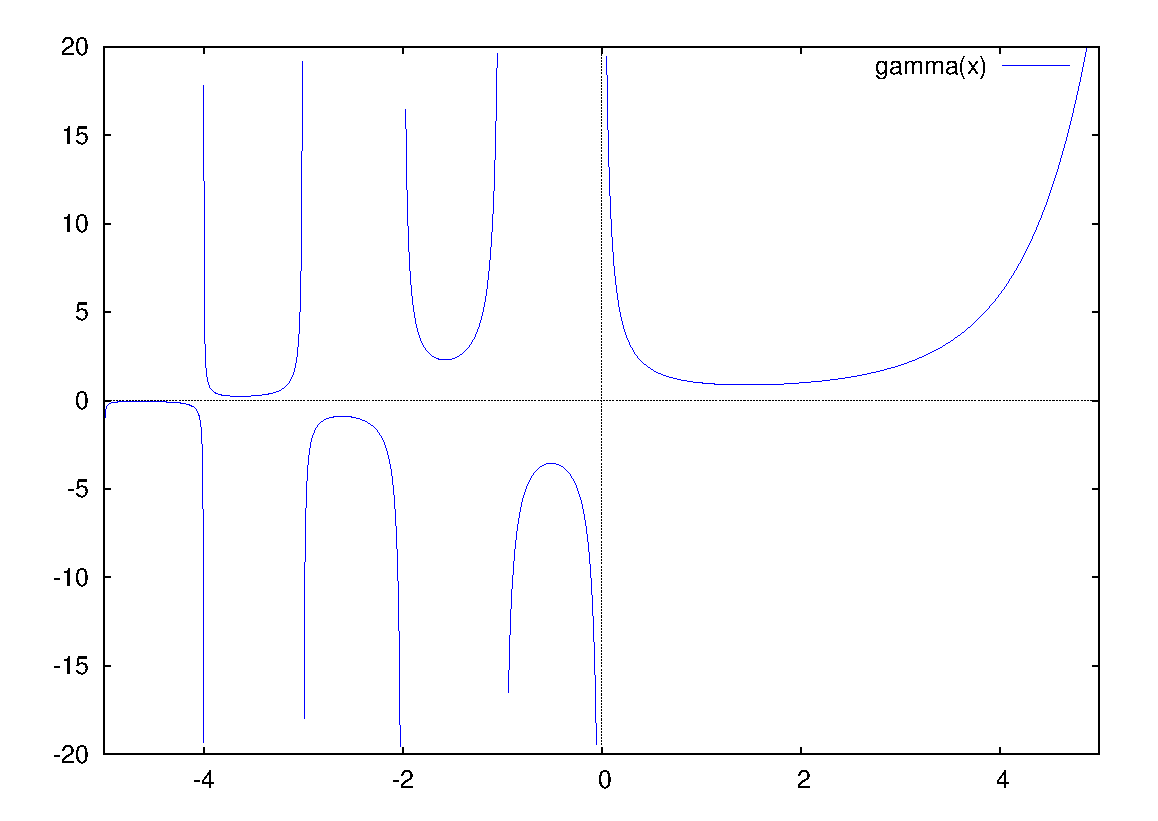
\includegraphics[width=.5\linewidth]{images/gamma} \end{center}

\litem{Beta function}{C\&B eq.~3.3.17}\index{B(.) (Beta function)@$ B ( \cdot ) $ (Beta function)} $ B (\alpha, \beta) \equiv \Gamma (\alpha) \cdot \Gamma (\beta) / \Gamma (\alpha + \beta) $.

\litem{Logistic function}{D\&M 515; Metrics P.S. 5-4a}
\[ \Lambda (x) \equiv (1 + e^{-x})^{-1} \equiv \frac{e^x}{1 + e^x}. \]
Inverse is $ \Lambda^{-1}(\mu) \equiv \ell(\mu) \equiv \ln [\mu / (1 - \mu)] $. First derivative
$$ \lambda(x) \equiv \Lambda'(x) \equiv \frac{e^x}{(1 + e^x)^2} = \Lambda(x) (1- \Lambda (x)) = \Lambda(x) \Lambda{-x} . $$

\litem{Taylor series}{C\&B 5.5.20--1} If $ g(x) $ has derivatives of order $ r $ (i.e., $ g^{(r)}(x) $ exists), then for any constant $ a $ the Taylor polynomial of order $ r $ about $ a $ is:
$$ g(x) \approx T_r (x) \equiv \sum_{i=0}^r \frac{g^{(i)}(a)}{i!}(x-a)^{i}. $$
The remainder from the approximation Taylor approximation, $ g(x) - T_r (x) $ equals $ \int_a^x g^{(r+1)}(t) \cdot (x-t)^r / r! \, dt $.
This error always tends to $ 0 $ faster than the highest-order explicit term---i.e., $ \lim_{x \to a} [g(x) - T_r(x)]/(x-a)^r = 0 $.

\litem{Derivative of power series}{Hansen 2-29}\index{Power series} If $ g(t) \equiv  a_0 + a_1 t + a_2 t^2 + \dotsb = \sum_i a_i t^i $, then
$$ \left. \frac{\partial^k}{\partial t^k} g(t) \right|_{t=0} = a_k k!. $$
This is useful for calculating moments if we can express the mgf as a power series.

\litem{Taylor series examples}{?}
$ f(x) \approx f(x') + \nabla f(x') \cdot (x - x') $. Note that for concave (convex) $ f (\cdot) $, the LHS is weakly less (greater) than the RHS.

For small $ \epsilon $, we have:
\begin{align*}
e^{n \epsilon} &\approx 1 + n \epsilon; \\
(1 + \alpha \epsilon)^n &\approx 1 + \alpha n \epsilon; \\
\ln (1+\epsilon) &\approx \epsilon; \\
\frac{a^\epsilon - 1}{\epsilon} &\approx \log a .
\end{align*}

Second-order is
\[ f(x) \approx f(x') + \nabla f(x') \cdot (x - x') + \tfrac{1}{2} (x - x') \cdot \nabla^2 f(x') (x - x') .  \]

\litem{Mean value expansion}{Mahajan 3-13; Hayashi 470--1} If $ h \colon \R^p \to \R^q $ is a continuously differentiable function, then $ h(\cdot) $ admits a mean value expansion about $ \theta $
$$ h(b) = h(\theta) + \tfrac{\partial h (\bar{b})}{\partial b} (b - \theta) $$
where $ \bar{b} $ is a value lying between $ b $ and $ \theta $ (note the MVT applies to individual elements of $ h(\cdot) $, so $ \bar{b} $ actually differs from element to element in the vector equation.

\subsection{Correspondences}
\litem{Correspondence}{Micro math 5} $ \phi \colon X \rightrightarrows Y $ is a mapping from elements of $ X $ to subsets of $ Y $ (i.e., for $ x \in X $, we have $ \phi(x) \subseteq Y $).

\litem{Lower semi-continuity}{Micro math 7; Clayton G.E.~I}\index{lsc (lower semi-continuity)}\index{lhc (lower hemi-continuity)}\index{Lower hemi-continuity} $ \phi \colon X \rightrightarrows Y $ is lower semi-/hemi-continuous at $ x \in X $ iff for every open set $ G \subseteq Y  $ containing $ \phi(x) $, there is an open set $ U(x) \subseteq X $ containing $ x $ such that if $ x' \in U(x) $, then $ \phi (x') \cap G \neq \emptyset $.

Intuitively, any element in $ \phi (x) $ can be ``approached'' from all directions.

For a single-valued correspondence (i.e., a function), lsc $ \iff $ usc $ \iff $ continuous.

\litem{Upper semi-continuity}{Micro math; Clayton G.E.~I; Bernheim 32}\index{usc (upper semi-continuity)}\index{uhc (upper hemi-continuity)}\index{Upper hemi-continuity} $ \phi \colon X \rightrightarrows Y $ is upper semi-/hemi-continuous at $ x \in X $ iff for every open set $ G \subseteq Y  $ containing $ \phi(x) $, there is an open set $ U(x) \subseteq X $ containing $ x $ such that if $ x' \in U(x) $, then $ \phi (x') \subset G $.

Identically, if for any sequences $ x_t \to x $ and $ y_t \to y $ with $ y_t \in \phi(x_t) $ for all $ t $, we have $ y \in \phi(x) $.

Intuitively, $ \phi (x) $ does not ``suddenly contain new points;'' i.e., the graph of the function is a closed set.

For a single-valued correspondence (i.e., a function), usc $ \iff $ lsc $ \iff $ continuous.

\litem{Brouwer's Fixed Point Theorem}{Clayton G.E.~I} If a function $ f \colon A \to A $ is continuous, and $ A $ is compact and convex, then $ f(x) = x $ for some fixed point $ x \in A $.

\litem{Kakutani's Fixed Point Theorem}{Clayton G.E.~I; Bernheim 32} Suppose $ S $ is compact and convex. $ \gamma \colon S \rightrightarrows S $ is convex-valued and upper semi-continuous. Then there exists a fixed point $ s^* \in S $ such that $ s^* \in \gamma(s^*) $.

\subsection{Linear algebra}
\litem{Matrix}{Amemiya Ch.~11} Matrix $ \mA_{n \times m} \equiv \{ a_{ij} \} $ has $ n $ rows and $ m $ columns.
\begin{enumerate}
\item Square\index{Square matrix} iff $ n = m $.
\item Transpose\index{Transpose}\index{Matrix transpose} $ \mA' \equiv \{ a_{ji} \} $ is $ m \times n $.
\item Symmetric\index{Symmetric matrix} iff square and $ \forall i, $ $ j $, $ a_{ij} = a_{ji} $, or equivalently iff $ \mA = \mA' $.
\item Diagonal\index{Diagonal matrix} iff $ \forall i \neq j $, $ a_{ij} = 0 $ (i.e., nondiagonal elements are 0).
\end{enumerate}

\litem{Matrix multiplication}{Amemiya Ch.~11}
If $ c $ is a scalar, $ c \mA = \mA c = \{ c a_{ij} \} $.
If $ \mA $ is $ n \times m $ and $ \mB $ is $ m \times r $, then $ \mC = \mA \mB $ is an $ n \times r $ matrix with $ c_{ij} = \sum_{k=1}^{m}a_{ik}b_{kj} $. If $ \mA \mB $ is defined, then $ ( \mA \mB )' = \mB' \mA' $.

\litem{Determinant}{Amemiya Ch.~11; Greene 23--6} $ | \mA | \equiv \sum_{i} (-1)^{i+j} a_{ij} | \mA_{ij} | $, where $ j $ is an arbitrarily chosen integer and $ \mA_{ij} $ is the matrix that deletes the $ i $th row and $ j $th column from $ \mA $.

This is the volume of the parallelotope with edges along the columns of $ \mA $.
\begin{enumerate}
\item Determinant of a $ 2 \times 2 $ matrix $ \mA $ is $ a_{11} a_{22} - a_{12} a_{21} $.
\item Determinant of a $ 3 \times 3 $ matrix $ \mA $ is $
  a_{11} a_{22} a_{33}
- a_{11} a_{32} a_{23}
- a_{21} a_{12} a_{33}
+ a_{21} a_{32} a_{13}
+ a_{31} a_{12} a_{23}
- a_{31} a_{22} a_{13}
$.
\item $ | \mA | = | \mA' | $.
\item For diagonal $ \mA $, $ | \mA | = \prod_i a_{ii} $; thus $ | \mI | = 1 $.
\item $ | c \mA_{n \times n} | = c^n | \mA | $.
\item If $ \mA $, $ \mB $ both $ n \times n $, then $ | \mA \mB | = | \mA | \, | \mB | $; together with $ | \mI | = 1 $, this gives $ | \mA^{-1} | = | \mA |^{-1} $.
\item If any column/row of $ \mA $ is all zeroes, $ | \mA | = 0 $; switching two adjacent columns/rows changes the sign of the determinant; if two c/rs are identical, the determinant is zero.
\item For any eigenvalue $ \lambda $, $ | \mA - \lambda \mI | = 0 $.
\item $ | \mA_{n \times n} | = \prod_i \lambda_i $ (i.e., determinant is the product of eigenvalues).
\end{enumerate}

\litem{Matrix inverse}{Amemiya Ch.~11; Greene 30--1} $ \mA^{-1}\mA = \mA \mA^{-1} = \mI $ for any matrix $ \mA $ such that $ | \mA | \neq 0 $.
\begin{enumerate}
\item If $ \mA $, $ \mB $ both $ n \times n $, and $ | \mA | \neq 0 $, $ | \mB | \neq 0 $, then $ (\mA \mB)^{-1} = \mB^{-1} \mA^{-1} $.
\item If $ \mA^{-1} $ exists, then $ (\mA^{-1})' = (\mA')^{-1} $.
\item The inverse of a $ 2 \times 2 $ matrix is
$$ \begin{bmatrix}
a & b \\
c & d
\end{bmatrix}^{-1} =
\frac{1}{| \mA |}
\begin{bmatrix}
d & -b \\
-c & a
\end{bmatrix}
=
\frac{1}{ad - bc}
\begin{bmatrix}
d & -b \\
-c & a
\end{bmatrix} . $$
\item For diagonal $ \mA $, the inverse is diagonal with elements $ a_{ii}^{-1} $.
\end{enumerate}

\litem{Orthogonal matrix}{Amemiya Ch.~11} A square matrix $ \mA_{n \times n} $ is orthogonal iff $ \mA' = \mA^{-1} $. This corresponds to having columns orthogonal and normalized.

\litem{Trace}{Amemiya Ch.~11; Metrics section; Greene 41--2} $ \operatorname{tr}(\mA_{n \times n}) \equiv \sum_i a_{ii} $ (i.e., the sum of the diagonal elements).
\begin{enumerate}
\item $ \operatorname{tr}(c \mA) = c \operatorname{tr}(\mA) $.
\item $ \operatorname{tr}(\mA') = \operatorname{tr}(\mA) $.
\item $ \operatorname{tr}(\mA + \mB) = \operatorname{tr}(\mA) + \operatorname{tr}(\mB) $.
\item $ \operatorname{tr}(\mA_{n \times m} \mB_{m \times n}) = \operatorname{tr}(\mB \mA) $.
\item Trace is the sum of eigenvalues: $ \operatorname{tr}(\mA_{n \times n}) = \sum_i \lambda_i $.
\item $ \operatorname{tr}(\mA_{n \times m} \mA') = \operatorname{tr}(\mA' \mA) = \sum_{i=1}^{n} \sum_{j=1}^{m} a_{ij}^2 = \sum_{j=1}^{m} a_{j}' a_j =  \sum_{j=1}^{m} \operatorname{tr} (a_{j} a_{j}') $, where $ a_i $ are the columns of $ \mA $.
\end{enumerate}
\textit{Caution}: in general, $ \operatorname{tr}(\mA  \mB) \neq \operatorname{tr}(\mA) \cdot \operatorname{tr}(\mB) $.

\litem{Linear independence, rank}{Amemiya Ch.~11; Greene 20--3, 39}\index{Rank} Vectors $ \{ \mx_i \} $ linearly independent iff $ \sum_i c_i \mx_i = 0 \implies \forall i $, $ c_i = 0 $.
\begin{enumerate}
\item The following are equivalent and called nonsingularity of square $ \mA $\index{Nonsingularity}\index{Singularity}:
\begin{itemize}
\item $ | \mA | \neq 0 $, $ \mA^{-1} $ exists;
\item $ \mA $ is column independent or row independent;
\item $ \forall \mathbf{y} $, $ \exists \mx $, $ \mA \mx = \mathbf{y} $;
\item $ \mA \mx = \mzero \implies \mx = \mzero $.
\end{itemize}
\item Column rank (maximum number of linearly independent columns) equals row rank, which implies $ \rank \mA = \rank \mA' $.
\item $ \mA_{n \times m} $ is full rank iff rank equals $ \min (n, m) $; a square matrix is full rank iff it is nonsingular.
\item $ \rank (\mA) = \rank (\mA' \mA) = \rank (\mA \mA') $; in particular, $ \mA_{n \times m} $ with $ m \leq n $ (i.e., ``tall'') is full rank iff $ \mA' \mA $ is nonsingular.
\item $ \mA $ is nonsingular $ \implies \rank (\mA \mB) = \rank (\mB) $.
\item $ \rank (\mA_{n \times n}) $ equals the number of nonzero eigenvalues (not necessarily distinct).
\end{enumerate}

\litem{Eigen decomposition}{Mathworld} For any square $ \mA $ with $ \mathbf{\Lambda} $ a diagonal matrix containing eigenvalues of $ \mA $, and $ \mathbf{P} $ a matrix whose columns are the eigenvectors of $ \mA $ (ordered as in $ \mathbf{\Lambda} $), then $ \mA = \mathbf{P} \mathbf{\Lambda} \mathbf{P}^{-1} $.

\litem{Orthogonal decomposition}{Amemiya Ch.~11; Greene 37--8} a.k.a.\ spectral decomposition\index{Spectral decomposition}. For any symmetric $ \mA $, $ \exists \mathbf{H}_{n \times n} $, $ \mathbf{\Lambda}_{n \times n} $ such that $ \mA = \mathbf{H} \mathbf{\Lambda} \mathbf{H}' $, where $ \mathbf{H}' \mathbf{H} = \mI $ (i.e., $ \mathbf{H} $ is orthogonal) and $ \mathbf{\Lambda} $ is diagonal. Note that $ \mathbf{H}' \mA \mathbf{H} = \mathbf{\Lambda} $.

This is just the eigen decomposition for a symmetric matrix; here the matrix of eigenvectors is orthogonal.

\litem{Matrix squareroot}{Greene 42} Given a positive definite symmetric matrix $ \mA = \mathbf{H} \mathbf{\Lambda} \mathbf{H}' $, we can get a (symmetric!) matrix squareroot $ \mA^{1/2} \equiv \mathbf{H} \mathbf{\Lambda}^{1/2} \mathbf{H}' $, where $ \mathbf{\Lambda}^{1/2} $ is the diagonal matrix that takes the squareroot of diagonal elements of $ \mathbf{\Lambda} $.

\litem{Eigenvector, eigenvalue}{Amemiya Ch.~11; Woodford 670--2}\index{Eigenvector}\index{Eigenvalue}\index{Characteristic root}\index{Characteristic vector} Note some results may only hold for symmetric matrices (not made explicit in Amemiya). Let the orthogonal decomposition of symmetric $ \mA $ be $ \mA = \mathbf{H} \mathbf{\Lambda} \mathbf{H}' $, where $ \mathbf{H} $ is orthogonal and $ \mathbf{\Lambda} $ is diagonal.
\begin{enumerate}
\item Diagonal elements of $ \mathbf{\Lambda} \equiv \mathbf{D}(\lambda_i) $ are eigenvalues (a.k.a.\ characteristic roots) of $ \mA $; columns of $ \mathbf{H} $ are the corresponding eigenvectors (a.k.a.\ characteristic vectors).
\item If $ \mathbf{h} $ is the eigenvector corresponding to $ \lambda $, then $ \mA \mathbf{h} = \lambda \mathbf{h} $ and $ | \mA - \lambda \mI | = 0 $. (This is an alternate definition for eigenvectors/eigenvalues.)
\item Matrix operations $ f(\mA) $ can be reduced to the corresponding scalar operation: $ f(\mA) = \mathbf{H} \mathbf{D}[f(\lambda_i)] \mathbf{H}' $.
\item $ \rank (\mA_{n \times n}) $ equals the number of nonzero eigenvalues (not necessarily distinct).
\item $ \mA_{n \times m} \mB_{m \times n} $ and $ \mB \mA $ have the same nonzero eigenvalues.
\item Symmetric $ \mA_{n \times n} $ and $ \mB_{n \times n} $ can be diagonalized by the same orthogonal matrix $ \mathbf{H} $ iff $ \mA \mB = \mB \mA $.
\item $ | \mA_{n \times n} | = \prod_i \lambda_i $ (i.e., determinant is the product of eigenvalues).
\item $ \operatorname{tr}(\mA_{n \times n}) = \sum_i \lambda_i $ (i.e., trace is the sum of eigenvalues).
\item $ \mA $ and $ \mA^{-1} $ have same eigenvectors and inverse eigenvalues.
\end{enumerate}

A $ 2 \times 2 $ matrix $ \mA $ has two explosive eigenvalues (outside the unit circle) iff either
\begin{itemize}
\item Case I:
\begin{align*}
| \mA | + \operatorname{tr} \mA &\geq -1 , \\
| \mA | - \operatorname{tr} \mA &\geq -1 , \\
| \mA | \phantom{{} + \operatorname{tr} \mA} &\leq \phantom{-} 1 .
\end{align*}
\item Case II:
\begin{align*}
| \mA | + \operatorname{tr} \mA &\leq -1 , \\
| \mA | - \operatorname{tr} \mA &\leq -1 , \\
| \mA | \phantom{{} + \operatorname{tr} \mA} &\leq \phantom{-} 1 \quad \text{ (trivially)}.
\end{align*}
\end{itemize}

\litem{Positive definiteness, \&c.}{Amemiya Ch.~11; Greene 46--9} Symmetric $ \mA $ is positive definite iff $ \forall \mx \neq 0 $, $ \mx' \mA \mx > 0 $. Also written $ \mA > \mzero $; if $ \mA - \mB $ is positive definite, write $ \mA > \mB $. If equality isn't strict, $ \mA $ is positive semidefinite (a.k.a.\ nonnegative definite). Negative definite and negative semidefinite (a.k.a.\ nonpositive definite) similarly defined.
\begin{enumerate}
\item A symmetric matrix is positive definite iff its eigenvalues are all positive; similar for other (semi-)definiteness.
\item If $ \mA > \mzero $, all diagonal elements are $ >0 $ (consider a quadratic form with a unit vector).
\item $ \mB' \mB \geq \mzero $; if $ \mB $ has full column rank, then $ \mB' \mB > \mzero $.
\item $ \mA > \mzero \implies \mA^{-1} > \mzero $ (i.e., the inverse of a positive definite matrix is positive definite).
\item $ \forall \mB_{n \times k} $ ``tall'' (i.e., $ n \geq k $), $ \mA_{n \times n} \geq \mzero \implies \mB' \mA \mB \geq \mzero $. If $ \mB $ is full rank (i.e., $ \rank(\mB) = k $), then $ \mA_{n \times n} > \mzero \implies \mB' \mA \mB > \mzero $.
\item For $ \mA_{n \times n} $ and $ \mB_{n \times n} $ both positive definite, $ \mA \geq \mB \iff \mB^{-1} \geq \mA^{-1} $, and $ \mA > \mB \iff \mB^{-1} > \mA^{-1} $.
\item $ \mA \geq \mzero \implies \lvert \mA \rvert \geq 0 $ and $ \mA > \mzero \implies \lvert \mA \rvert > 0 $---note the natural analogues for negative (semi)definite matrices do \textit{not} hold.
\end{enumerate}

\litem{Orthogonal completion}{Hansen 5-24} For a ``wide'' matrix $ \mA_{n \times k} $ (i.e., $ n < k $) with full row rank (i.e., all rows are linearly independent), we can construct a (non-unique) $ (k - n) \times k $ matrix $ \mA_\perp $ such that:
\begin{enumerate}
\item The rows of $ \mA $ and $ \mA_\perp $ are linearly independent (i.e., $ | (\mA', \mA_{\perp}' ) | \neq 0 $;
\item The rows of $ \mA_\perp $ are orthogonal to the rows of $ \mA $ (i.e., $ \mA_\perp \mA' = \mzero_{k-n \times n} $, or identically, $ \mA \mA_{\perp}' = \mzero_{n \times k-n} $).
\end{enumerate}
For a ``tall'' matrix $ \mB_{n \times k} $ (i.e., $ n > k $) with full column rank (i.e., all columns are linearly independent), we can construct a (non-unique) $ n \times (n - k) $ matrix $ \mB_\perp $ such that:
\begin{enumerate}
\item The columns of $ \mB $ and $ \mB_\perp $ are linearly independent (i.e., $ | (\mB, \mB_{\perp} ) | \neq 0 $;
\item The columns of $ \mB_\perp $ are orthogonal to the columns of $ \mB $ (i.e., $ \mB_{\perp}' \mB = \mzero_{n-k \times k} $, or identically, $ \mB' \mB_{\perp} = \mzero_{k \times n-k} $).
\end{enumerate}

\litem{Idempotent matrix}{Hansen 5-33--4; Amemiya 37; Hayashi 30--1, 36--7, 244-5} $ \mathbf{P} $ is idempotent iff $ \mathbf{P} \mathbf{P} = \mathbf{P} $.
\begin{enumerate}
\item If $ \mathbf{P} $ is idempotent, then so is $ \mI - \mathbf{P} $.
\item Every eigenvalue of a (symmetric?) idempotent matrix is either $ 0 $ or $ 1 $.
\item A symmetric and idempotent matrix is positive semidefinite.
\item For any $ \mX_{n \times k} $, we can find an idempotent projection matrix (that projects onto the subspace of $ \R^n $ spanned by the columns of $ \mX $): $ \mathbf{P}_{\mX} \equiv \mX (\mX' \mX)^{-1} \mX' $.
\item For any $ \mX_{n \times k} $ tall (i.e., $ n > k $), we can find an idempotent projection matrix (that projects onto the subspace of $ \R^n $ \textit{not} spanned by columns of $ \mX $): $ \mI - \mathbf{P}_{\mX} = \mathbf{P}_{\mX_\perp} $.
\item $ \rank (\mathbf{P}) = \operatorname{tr}(\mathbf{P}) $ if $ \mathbf{P} $ is idempotent.
\end{enumerate}

\litem{Matrix derivatives}{Ying handout; Greene 51--53; MaCurdy} [Note derivative convention may be transpose of MWG.]
\begin{enumerate}
\item $ \tfrac{\partial}{\partial \mx} \mA \mx = \mA' $.
\item $ \tfrac{\partial}{\partial \mx} \mx' \mA \mx = (\mA + \mA') \mx $.
\item $ \tfrac{\partial}{\partial \mA} \mx' \mA \mx = \mx \mx' $.
\item $ \tfrac{\partial}{\partial \mA} \log | \mA | = {\mA'}^{-1} $.
\item $ \tfrac{\partial}{\partial \mA^{-1}} \log | \mA | = - {\mA'} $.
\item $ \tfrac{\partial}{\partial w} \log | \mA | = | \mA |^{-1} \cdot \tfrac{\partial}{\partial w} | \mA | = \operatorname{tr} [\mA ^{-1} \cdot \tfrac{\partial}{\partial w} \mA ] $ (may require symmetric $ \mA $?).
\item $ \tfrac{\partial}{\partial w} \mA^{-1} = - \mA^{-1} [\tfrac{\partial}{\partial w} \mA] \mA^{-1} $ (may require symmetric $ \mA $?).
\end{enumerate}

\litem{Partitioned matrices}{Hayashi 670--673; Greene 32--3}
\begin{align*}
\left \lvert \begin{bmatrix}
\mA_{11} & \mA_{12}  \\
\mA_{21} & \mA_{22}
\end{bmatrix} \right \rvert
&= \lvert \mA_{22} \rvert \cdot  \lvert \mA_{11} - \mA_{12} \mA_{22}^{-1} \mA_{21} \rvert  \\
&= \lvert \mA_{11} \rvert \cdot  \lvert \mA_{22} - \mA_{21} \mA_{11}^{-1} \mA_{12} \rvert ;
\end{align*}
%
%Hayashi A.3
$$ \begin{bmatrix}
\mA_{11} & \cdots & \mA_{1N} \\
\vdots & \ddots & \vdots \\
\mA_{M1} & \cdots & \mA_{MN}
\end{bmatrix}
\begin{bmatrix}
\mc_{1}  \\
\vdots  \\
\mc_{N}
\end{bmatrix}
=
\begin{bmatrix}
\sum_i \mA_{1i} \mc_{i}  \\
\vdots  \\
\sum_i \mA_{Mi} \mc_{i}
\end{bmatrix}; $$
%
%Hayashi A.4
$$ \begin{bmatrix}
\mA_{11} &  &  \\
 & \ddots &  \\
 &  & \mA_{MM}
\end{bmatrix}
\begin{bmatrix}
\mc_{1}  \\
\vdots  \\
\mc_{N}
\end{bmatrix}
=
\begin{bmatrix}
\mA_{11} \mc_{1}  \\
\vdots  \\
\mA_{MM} \mc_{M}
\end{bmatrix}; $$
%
%Hayashi A.5
$$ \mA_\text{diag} \mB_\text{diag} =
\begin{bmatrix}
\mA_{11} \mB_{11} &  &  \\
 & \ddots &  \\
 &  & \mA_{MM} \mB_{MM}
\end{bmatrix};
$$
%
%Hayashi A.6
\begin{multline*}
\mA_{\text{diag}}' \mB \mA_{\text{diag}}
\\ =
\begin{bmatrix}
\mA_{11}' \mB_{11} \mA_{11} & \cdots & \mA_{11}' \mB_{1M} \mA_{MM} \\
\vdots & \ddots & \vdots \\
\mA_{MM}' \mB_{M1} \mA_{11} & \cdots & \mA_{MM}' \mB_{MM} \mA_{MM}
\end{bmatrix};
\end{multline*}
%
%Hayashi A.7
\begin{multline*}
\mA_{\text{diag}}' \mB \mc
\\ =
\begin{bmatrix}
\mA_{11}' \mB_{11} \mc_{1} + \dotsc + \mA_{11}' \mB_{1M} \mc_{M} \\
\vdots \\
\mA_{MM}' \mB_{M1} \mc_{1} + \dotsc + \mA_{MM}' \mB_{MM} \mc_{M}
\end{bmatrix};
\end{multline*}
%
%Hayashi A.9
$$ \mA_{\text{diag}}^{-1} = \begin{bmatrix}
\mA_{11}^{-1} &  &  \\
 & \ddots &  \\
 &  & \mA_{MM}^{-1}
\end{bmatrix}. $$
The inverse of a $ 2 \times 2 $ partitioned matrix is:
%
%Hayashi A.10
\begin{multline*}
\begin{bmatrix}
\mA_{11} & \mA_{12}  \\
\mA_{21} & \mA_{22}
\end{bmatrix}^{-1}
\\ =
\begin{bmatrix}
\mA_{11}^{-1} + \mA_{11}^{-1} \mA_{12} \mathbf{F}_2 \mA_{21} \mA_{11}^{-1} & -\mA_{11}^{-1} \mA_{12} \mathbf{F}_2  \\
- \mathbf{F}_2 \mA_{21} \mA_{11}^{-1} & \mathbf{F}_2
\end{bmatrix},
\end{multline*}
where $ \mathbf{F}_2 \equiv (\mA_{22} - \mA_{21} \mA_{11}^{-1} \mA_{12})^{-1} $. The upper left block can also be written as $ \mathbf{F}_1 \equiv (\mA_{11} - \mA_{12} \mA_{22}^{-1} \mA_{21})^{-1} $

\litem{Kronecker product}{Hayashi 673; Greene 34--5} For $ \mA_{M \times N} $ and $ \mB_{K \times L} $,
$$ \mA \otimes \mB = \begin{bmatrix}
a_{11} \mB & \cdots & a_{1N} \mB \\
\vdots & \ddots & \vdots \\
a_{M1} \mB & \cdots & a_{MN} \mB
\end{bmatrix} $$
is $ MK \times NL $. Operation is \textit{not} commutative.
\begin{enumerate}
\item $ (\mA \otimes \mB) (\mC \otimes \mD) = \mA \mC \otimes \mB \mD $ (assuming matrix multiplications are conformable);
\item $ (\mA \otimes \mB)' = \mA' \otimes \mB' $;
\item $ (\mA \otimes \mB)^{-1} = \mA^{-1} \otimes \mB^{-1} $;
\item $ \operatorname{tr} (\mA_{M \times M} \otimes \mB_{K \times K}) = \operatorname{tr} (\mA) \cdot \operatorname{tr} (\mB) $;
\item $ \lvert \mA_{M \times M} \otimes \mB_{K \times K} \rvert = \lvert \mA \rvert^{M} \cdot \lvert \mB \rvert^{K} $.
\end{enumerate}

\litem{Deviation from means}{Hansen 5-34--5; Greene 14--5} $ \mathbf{M}_{\mi} \mx $ is the vector of $ x_i - \bar{\mx} $, and $ \mx' \mathbf{M}_{\mi} \mx = \sum_{i} (x_i - \bar{\mx})^{2} $, where
\[ \mathbf{M}_{\mi} \equiv \mI - \mi (\mi' \mi)^{-1} \mi' = \mI - \tfrac{1}{n} \mi \mi' \]
is the symmetric idempotent matrix with $ 1 - \tfrac{1}{n} $ on diagonal, and $ - \tfrac{1}{n} $ off diagonal.\footnote{In Greene, $ \mathbf{M}_{\mi} $ is called $ \mathbf{M}^0 $.}
\end{description}
\end{multicols}

%\newpage % pagebreak to use instead of rule
\hrule % rule to use instead of page break
\begin{multicols}{2}
\section{References}
\begin{tabbing}
Amemiya \quad \quad \= Amemiya: Introduction to Econometrics and Statistics \\
Bernheim \> Bernheim: Economics 203 notes \\
C\&B \> Casella, Berger: Statistical Inference, 2~ed. \\
Choice \> Levin, Milgrom, Segal: Introduction to Choice Theory notes \\
Clayton \> Featherstone: Economics 202 section notes \\
Consumer \> Levin, Milgrom, Segal: Consumer Theory notes \\
D\&M \> Davidson, MacKinnon: Estimation and Inference in Econometrics \\
G.E. \> Levin: General Equilibrium notes \\
Greene \> Greene: Econometric Analysis, 3~ed. \\
Hansen \> Hansen: Economics 270\slash 271 notes \\
Hayashi \> Hayashi: Econometrics \\
Jackson \> Jackson: Economics 204 lectures \\
MaCurdy \> MaCurdy: Economics 272 notes \\
Mahajan \> Mahajan: Economics 270\slash 271 notes \\
Manuel \> Amador: Economics 211 lectures \\
Math camp \> Fan: Math camp lectures \\
MathWorld \>  \texttt{mathworld.wolfram.com} \\
Max notes \> Floetotto: Economics 210 section \\
Micro Math \>  Levin, Rangel: Useful Math for Microeconomists notes  \\
MWG \> Mas-Collell, Whinston, Green: Microeconomic Theory \\
Nir \> Jaimovich: Economics 210 notes \\
Producer \> Levin, Milgrom, Segal: Producer Theory notes \\
Taylor \> Taylor: Economics 212 notes \\
Uncertainty \> Levin: Choice Under Uncertainty notes \\
Wikipedia \> \texttt{wikipedia.com} \\
Woodford \> Woodford: Interest and Prices
\end{tabbing}
\end{multicols}
\printindex
%\section{Statistical tables}
\addcontentsline{toc}{section}{Statistical tables}
\begin{center}
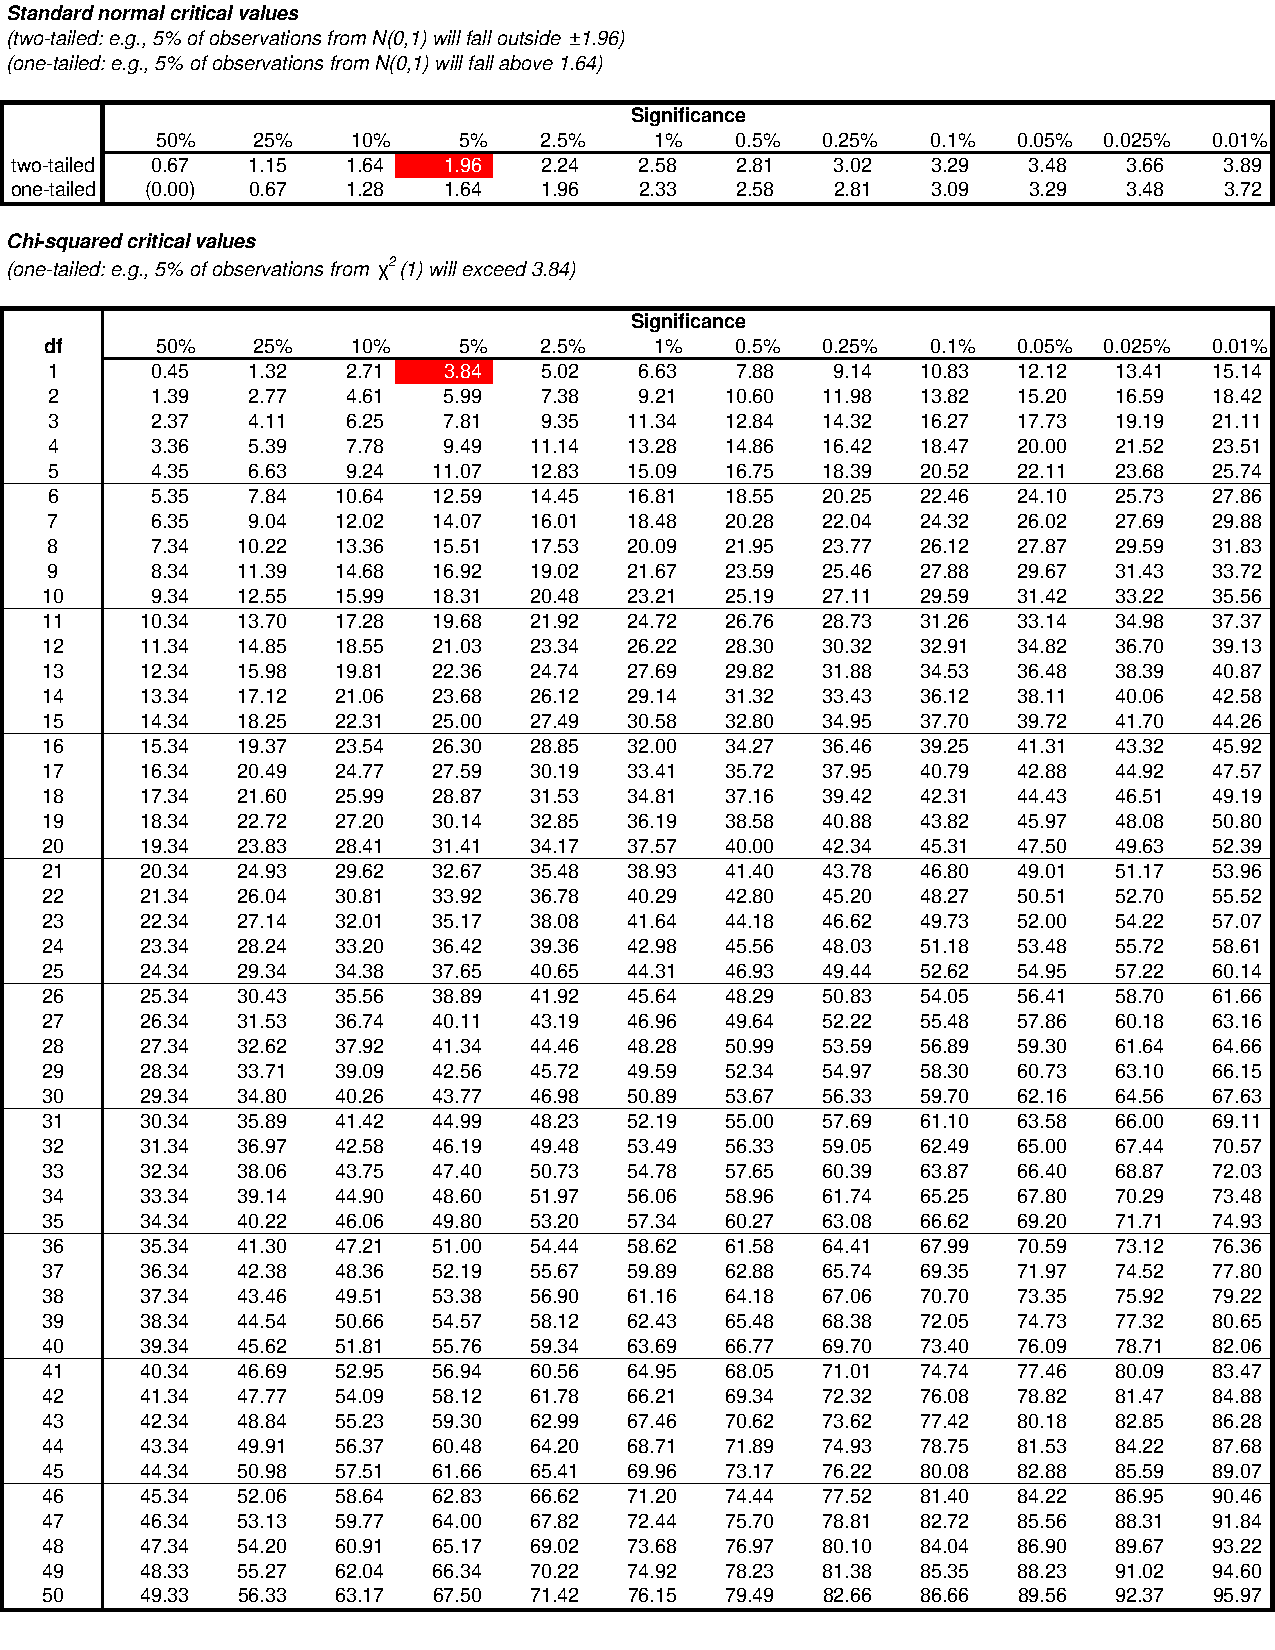
\includegraphics[height=9.75in, angle=90]{images/cv1}
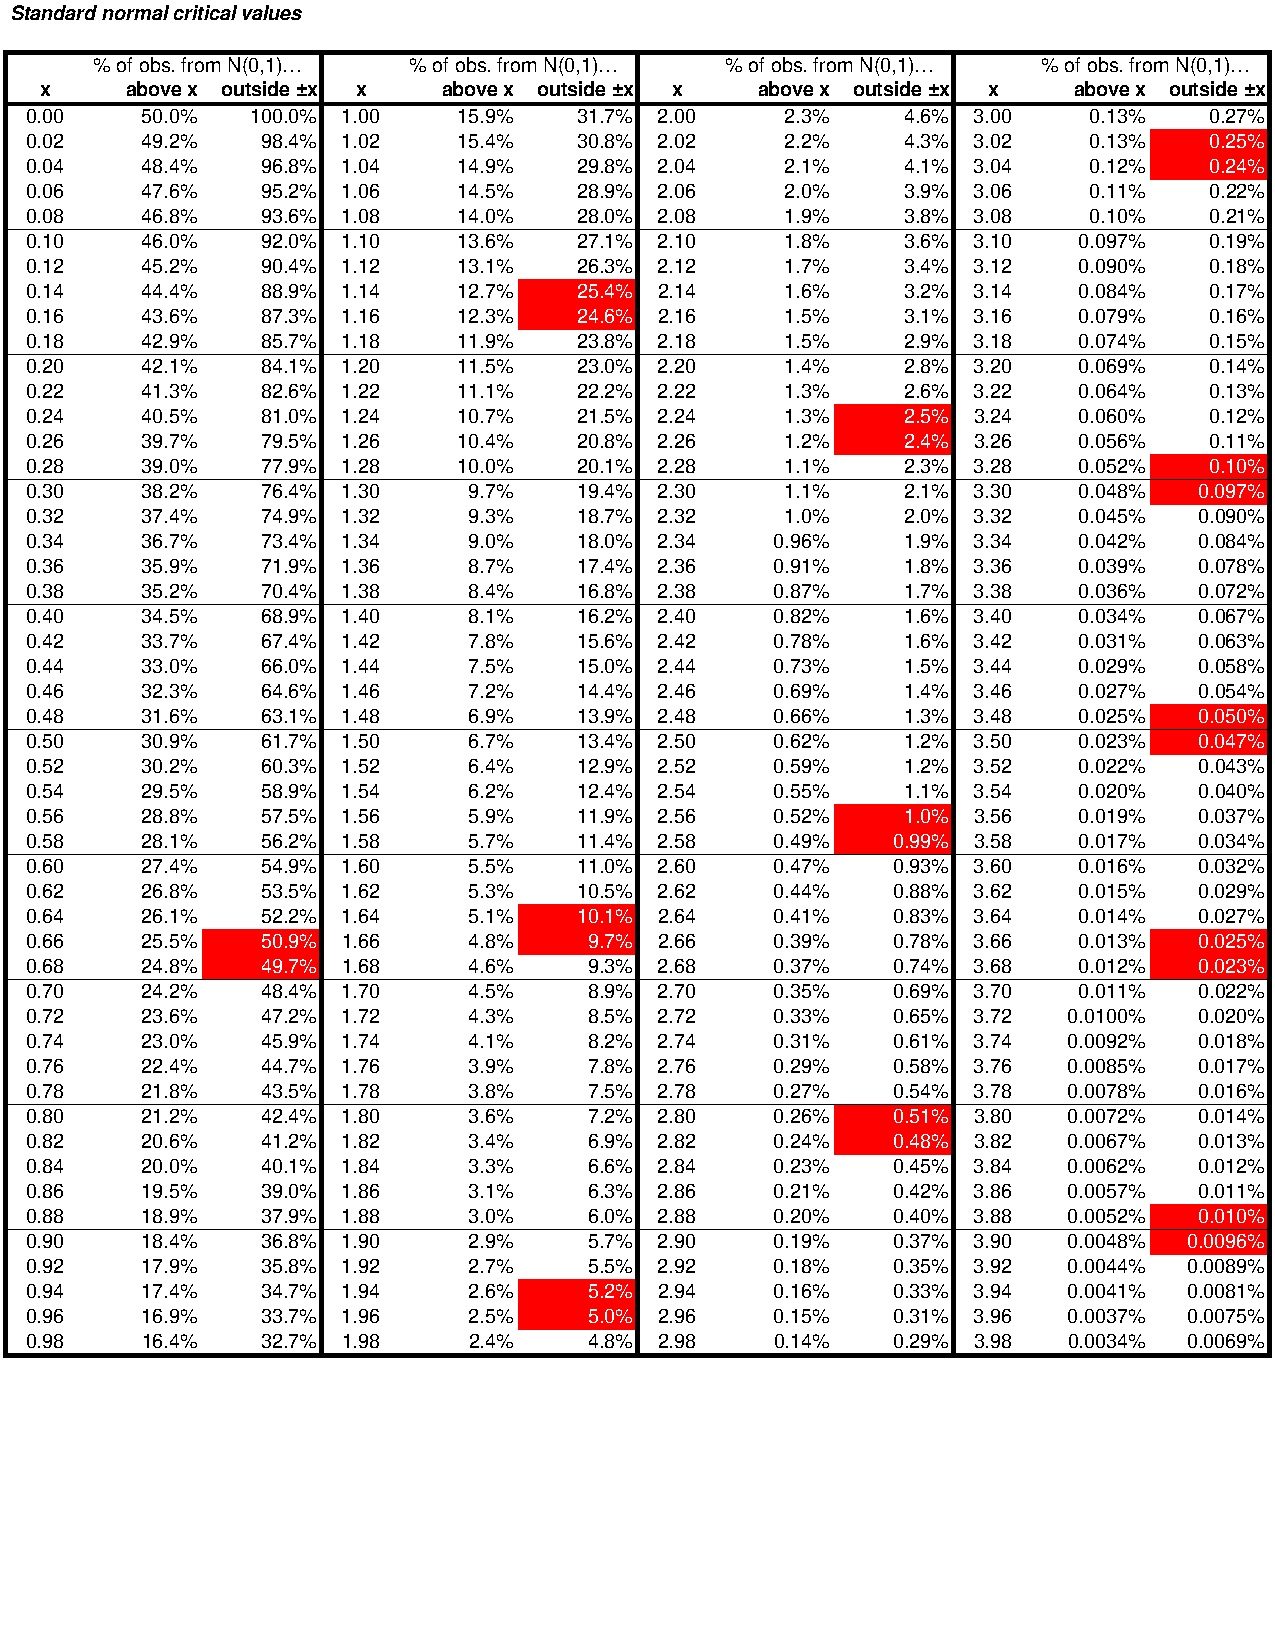
\includegraphics[height=9.75in, angle=90]{images/cv2}
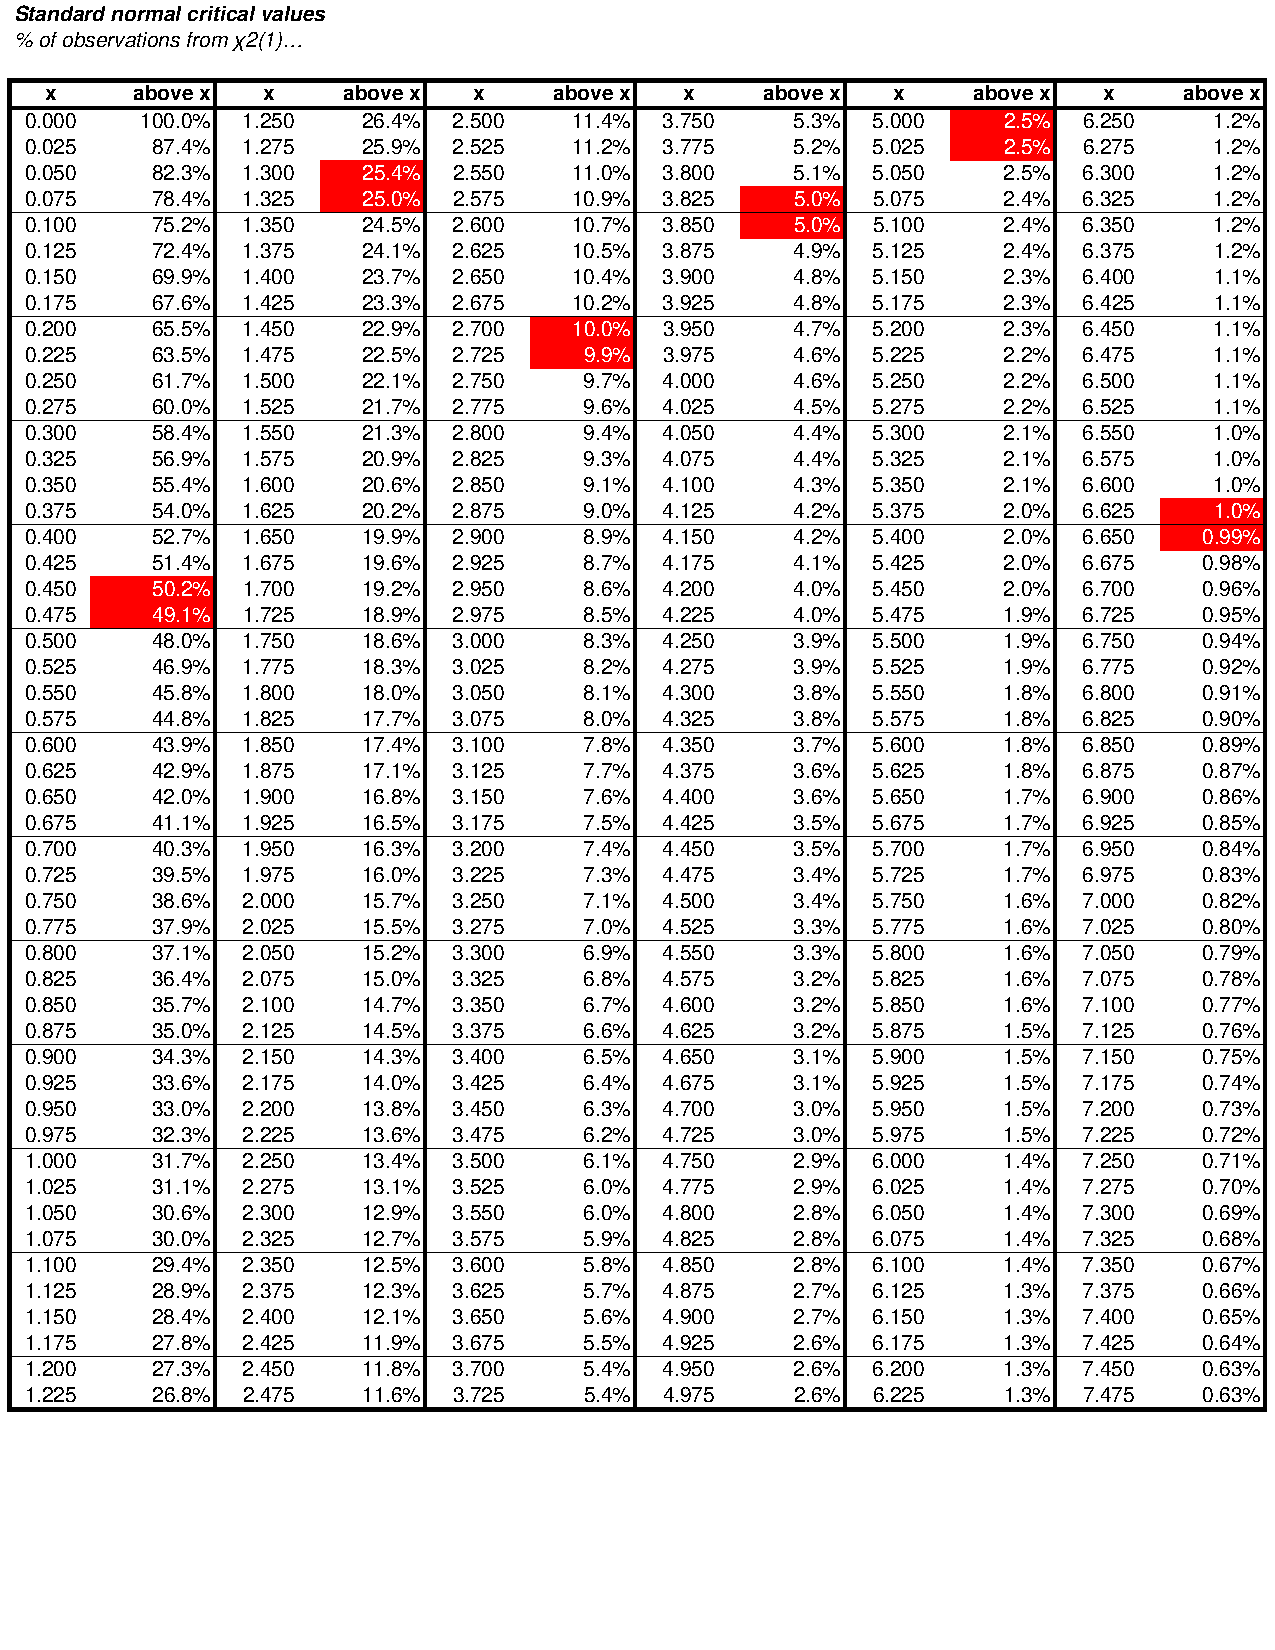
\includegraphics[height=9.75in, angle=90]{images/cv3}
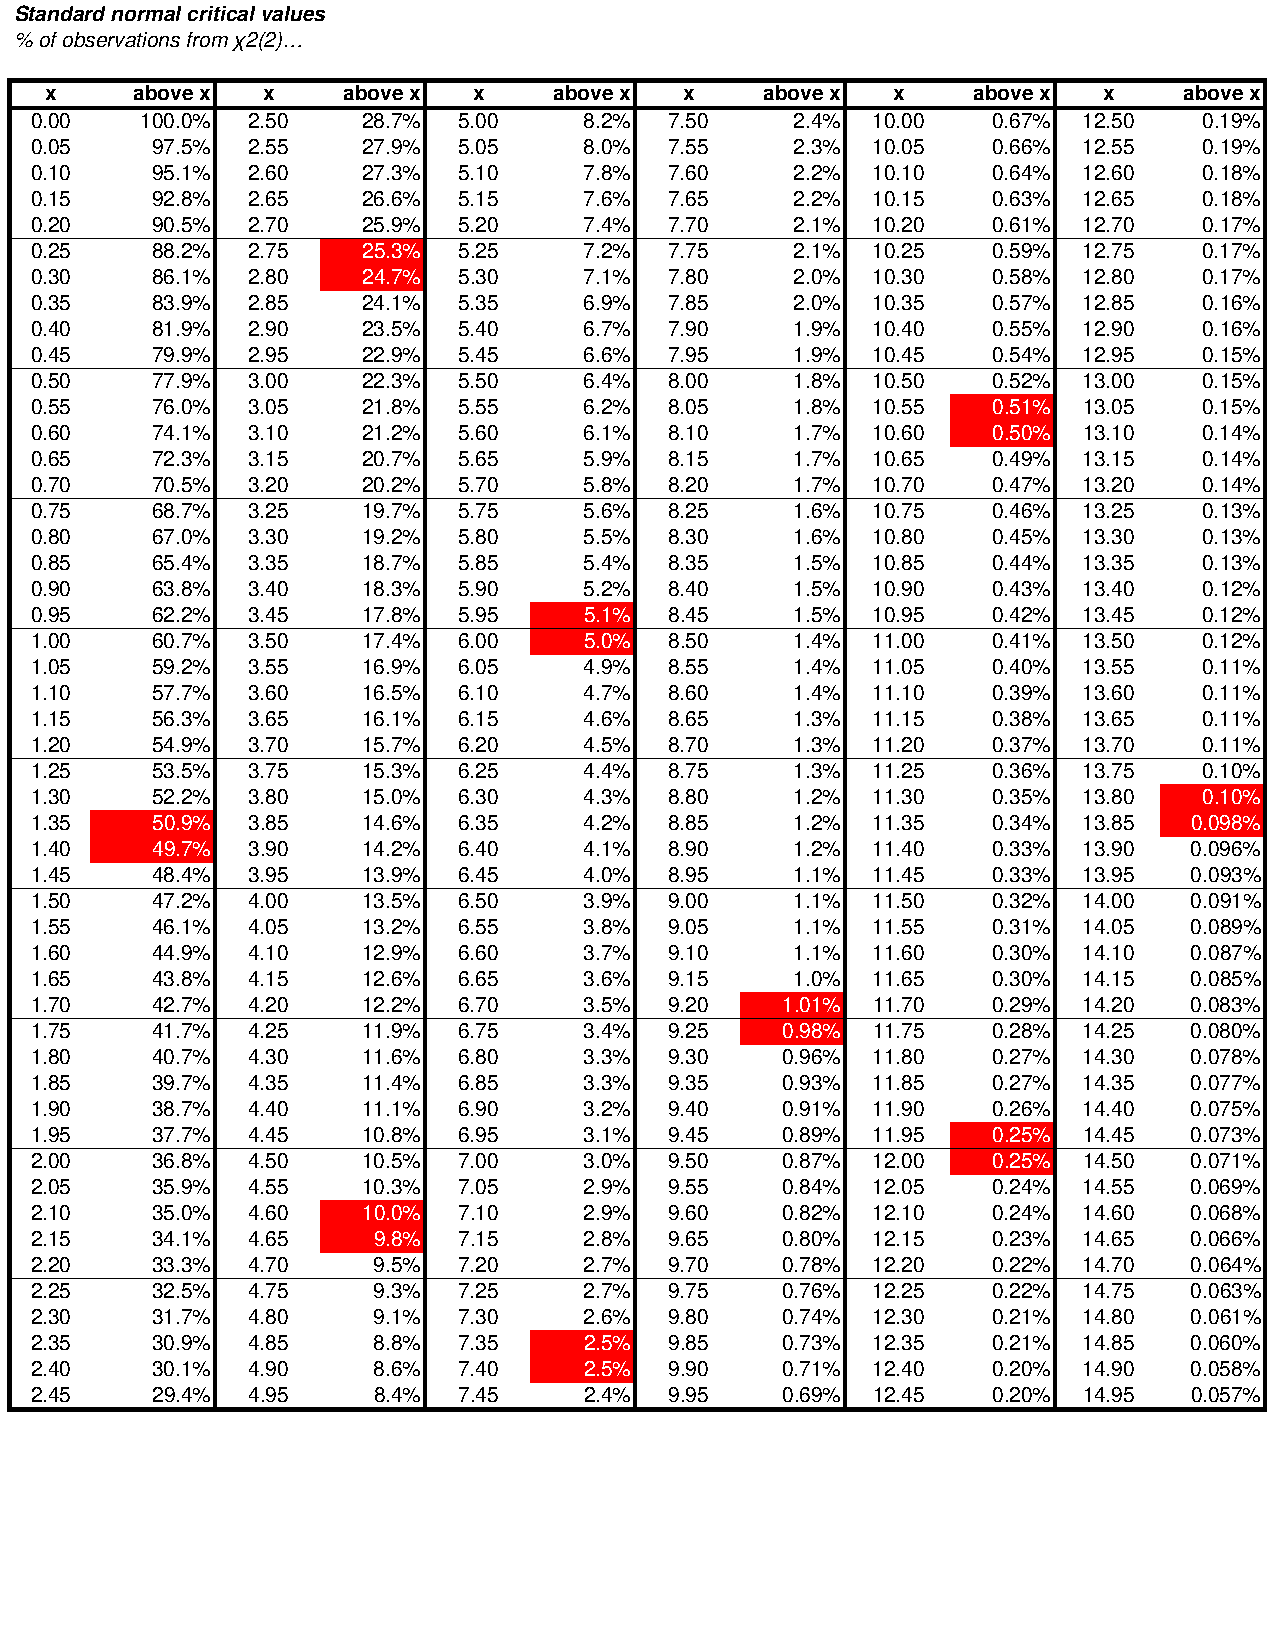
\includegraphics[height=9.75in, angle=90]{images/cv4}
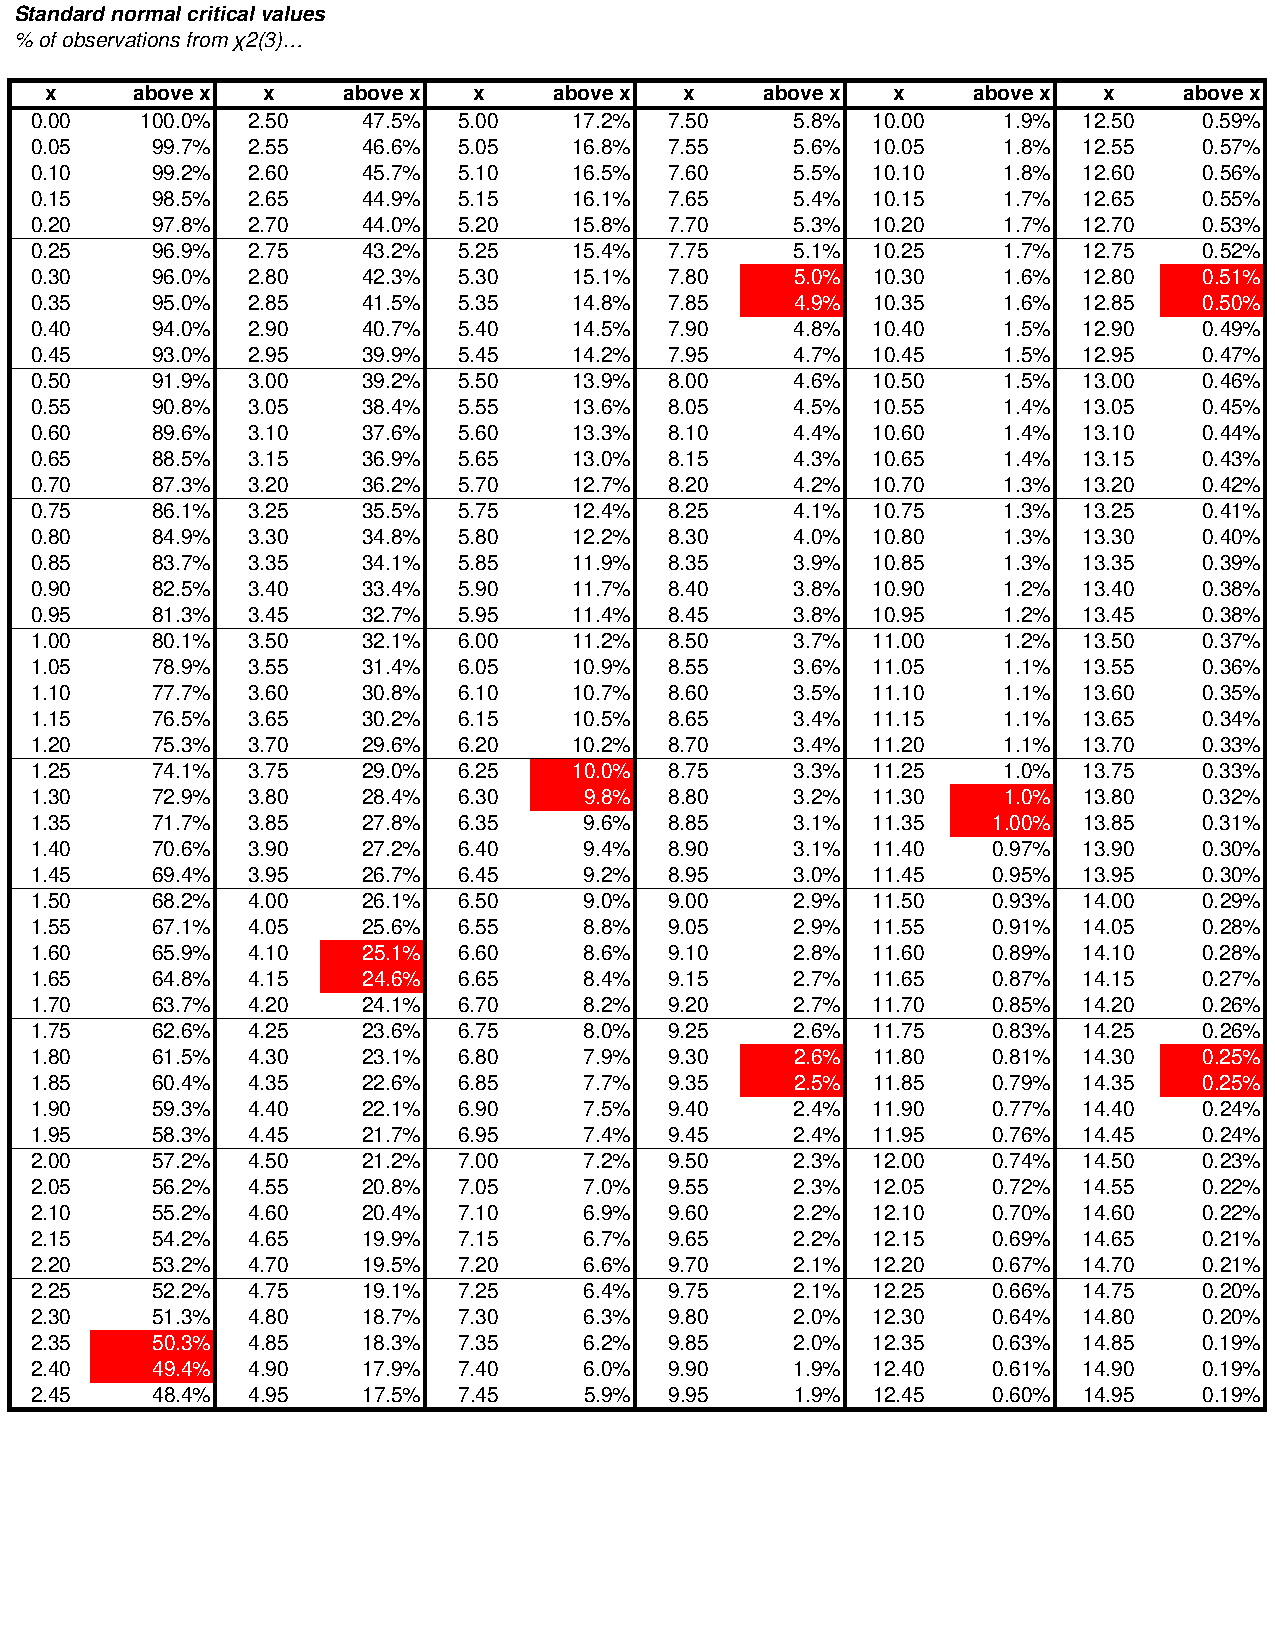
\includegraphics[height=9.75in, angle=90]{images/cv5}
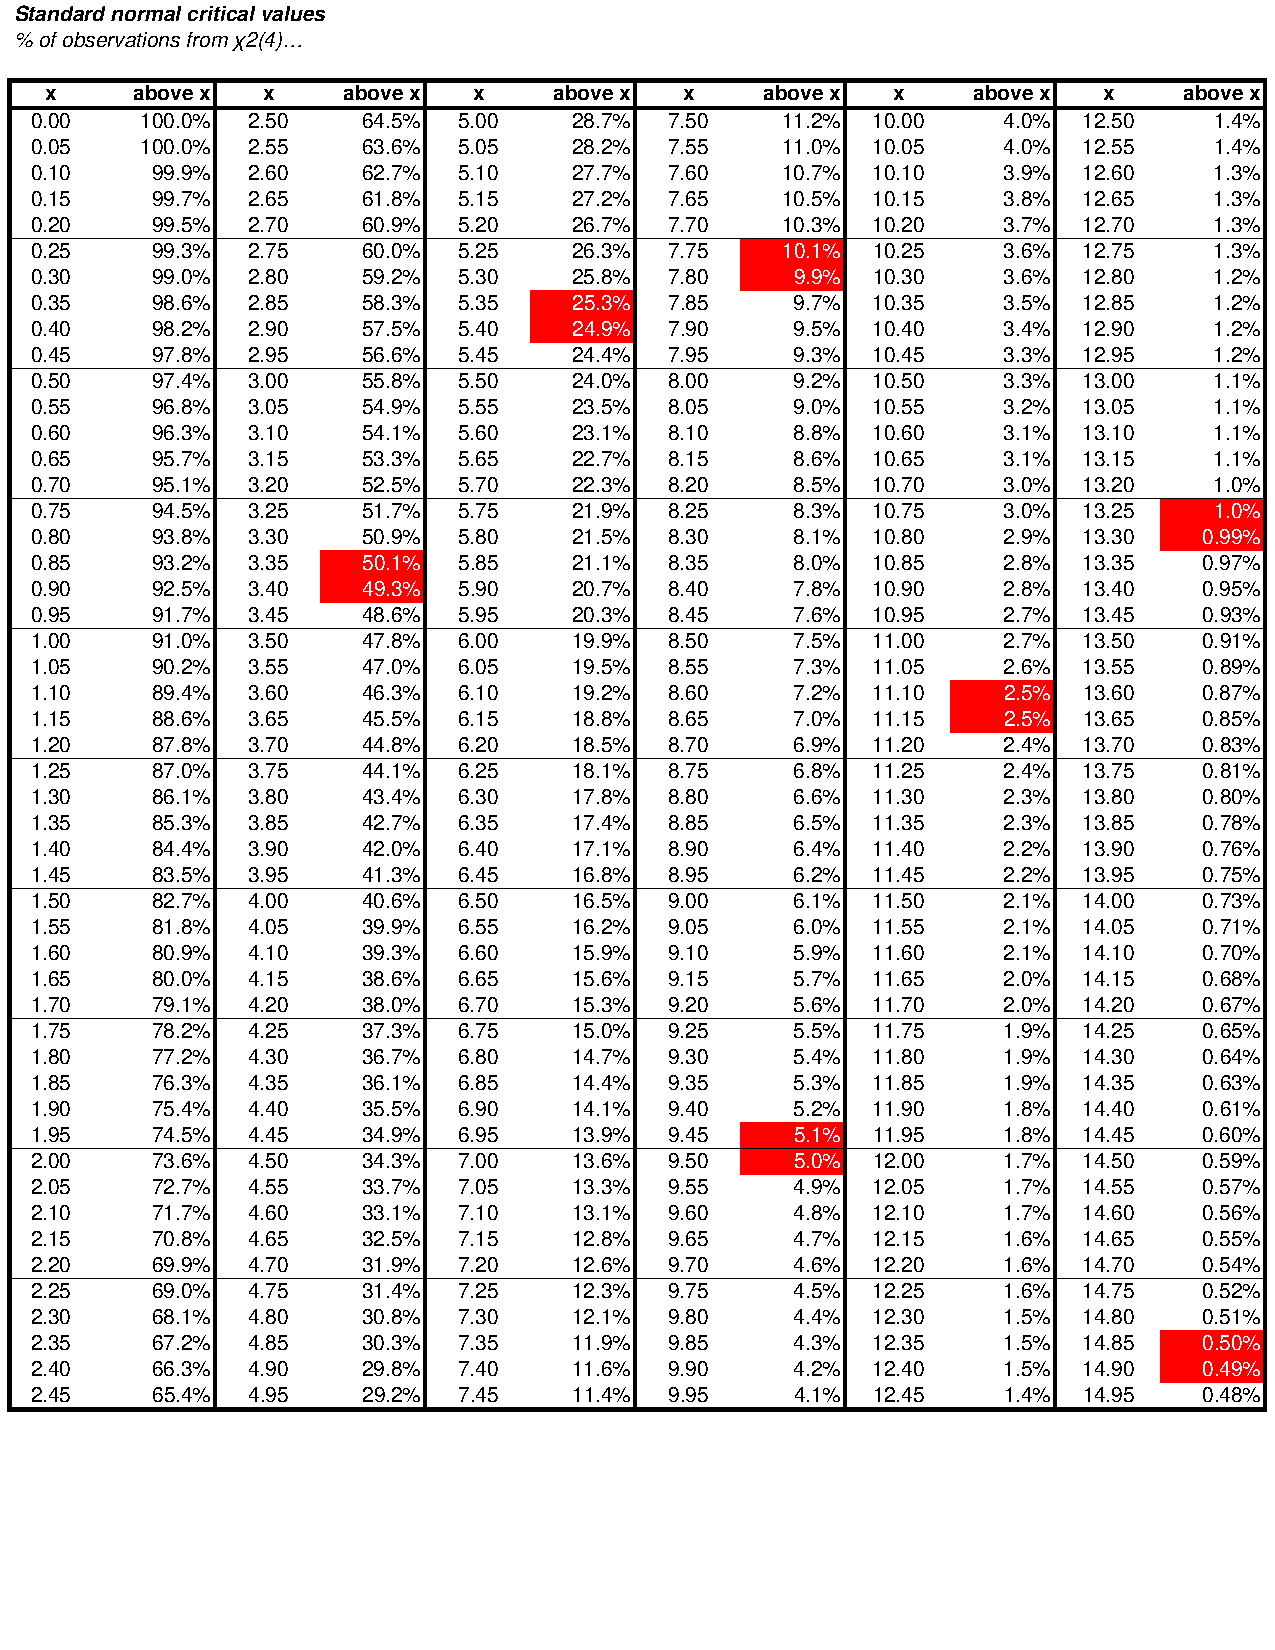
\includegraphics[height=9.75in, angle=90]{images/cv6}
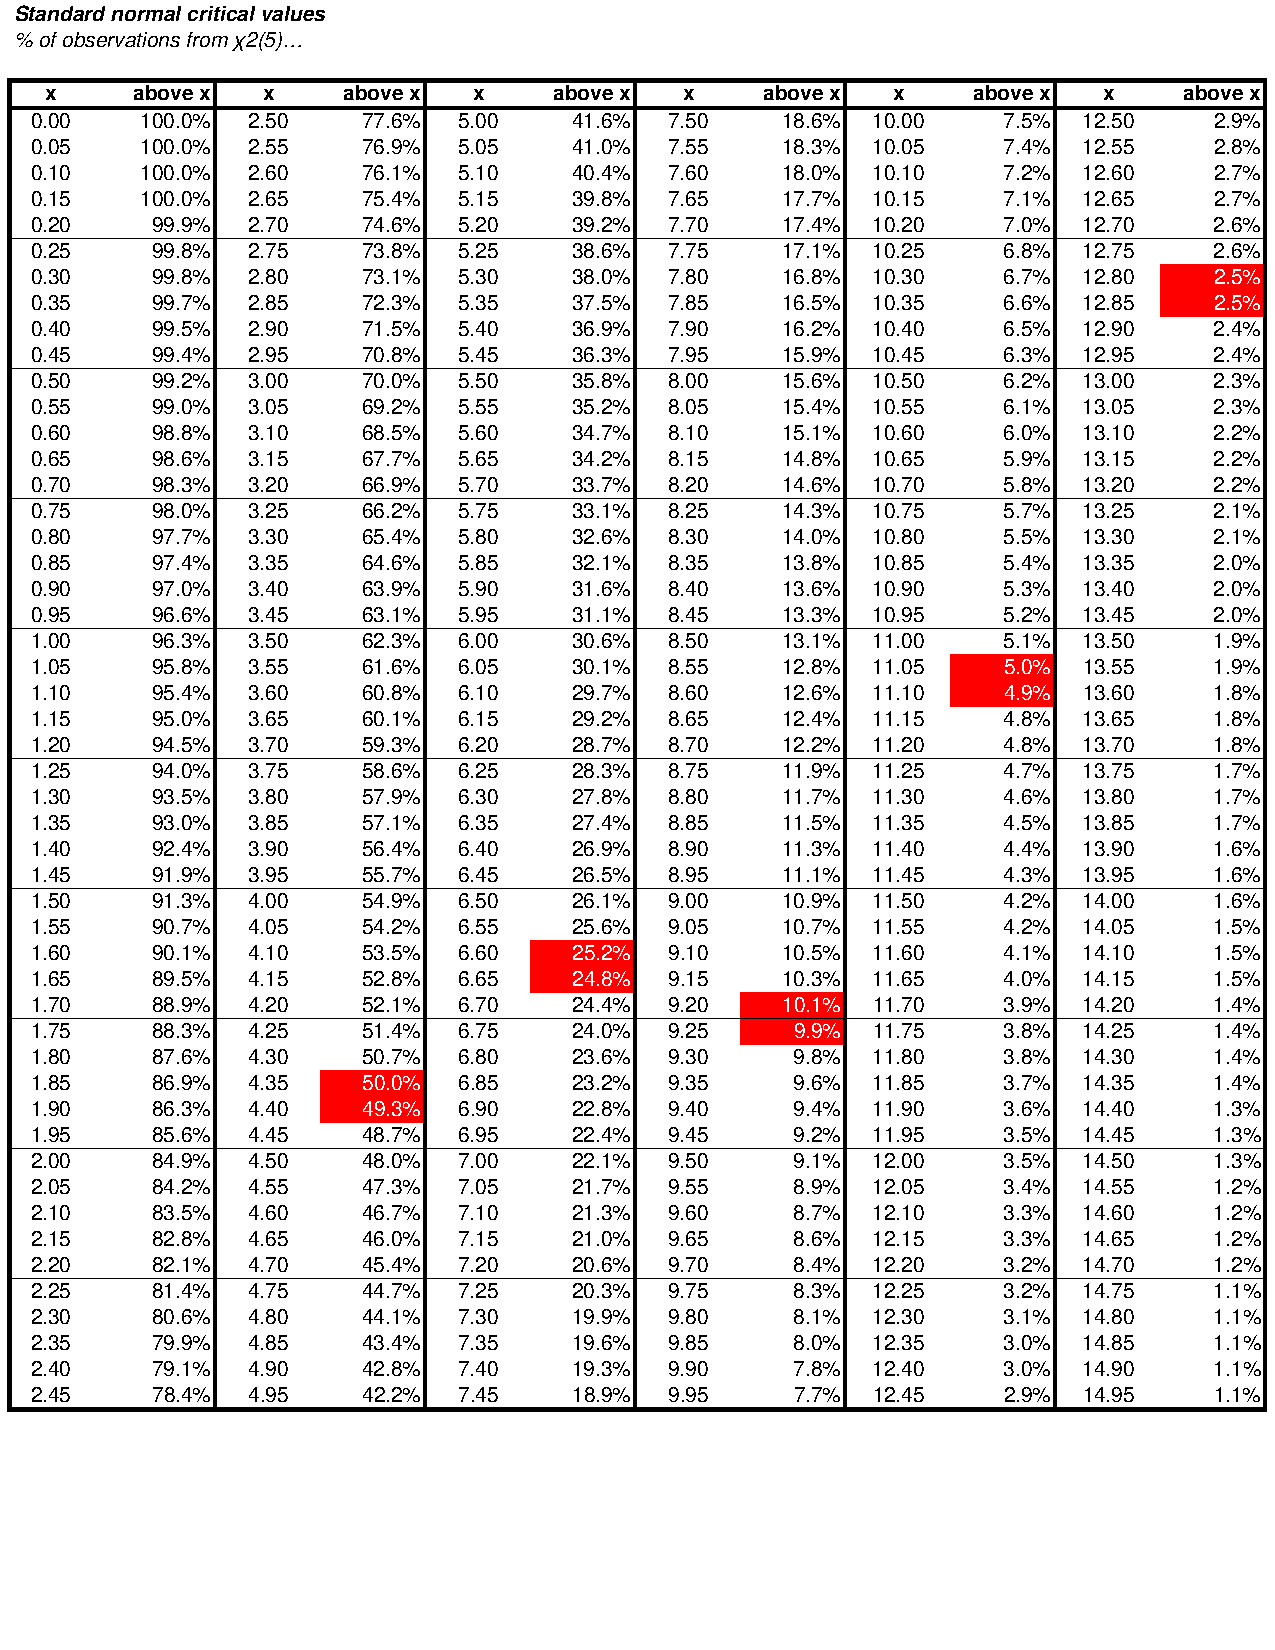
\includegraphics[height=9.75in, angle=90]{images/cv7}
\end{center}
\end{document}
